% Appendix list for Volume II --- the reference catalogues.
% The counterpart list for Volume I is appendix.tex. Between them every
% appendix file is input exactly once, so nothing is duplicated across the two
% volumes and nothing is orphaned.
\begin{appendices}
\renewcommand{\thesection}{\Alph{section}}
\titleformat{\section}{\normalfont\Large\bfseries}{Appendix \thesection}{1em}{}
\section{Functional Requirements Specification}
\label{appendix:fr}

% Specification tables are reference material, not prose: a step down in
% size and a tighter row stretch cost nothing in legibility and a great
% deal in printed bulk. The stretch is set here as well as on the
% individual tables, because not every table in this appendix declares one.
% Grouped so neither change leaks into the appendix that follows.
\begingroup
\small
\renewcommand{\arraystretch}{1.12}


\subsection{Specialized Project FRS}
This section contains the 57 functional requirements covered by Modules 1--4.

% ============================ Module 1: Authentication & Access Control ====================
\paragraph{Authentication and Access Control}

\renewcommand{\arraystretch}{1.12}
\begin{longtable}{|>{\centering\arraybackslash}m{0.05\textwidth}|m{0.29\textwidth}|>{\centering\arraybackslash}m{0.13\textwidth}|>{\centering\arraybackslash}m{0.13\textwidth}|>{\centering\arraybackslash}m{0.08\textwidth}|>{\centering\arraybackslash}m{0.08\textwidth}|>{\centering\arraybackslash}m{0.08\textwidth}|}
\caption{Functional Requirements for Authentication \& Access Control}
\label{tab:fr_auth_access} \\
\hline
\textbf{ID} & \multicolumn{1}{>{\centering\arraybackslash}m{0.29\textwidth}|}{\centering \textbf{Requirement}} & \textbf{\hspace{0pt}Users} & \textbf{User Requirement} & \textbf{\hspace{0pt}Fea\-si\-ble} & \textbf{\hspace{0pt}Test\-able} & \textbf{\hspace{0pt}Pri\-or\-ity} \\ \hline
\endfirsthead

\multicolumn{7}{c}%
{{\bfseries Table \thetable\ -- Continued from previous page}} \\
\hline
\textbf{ID} & \multicolumn{1}{>{\centering\arraybackslash}m{0.29\textwidth}|}{\centering \textbf{Requirement}} & \textbf{\hspace{0pt}Users} & \textbf{User Requirement} & \textbf{\hspace{0pt}Fea\-si\-ble} & \textbf{\hspace{0pt}Test\-able} & \textbf{\hspace{0pt}Pri\-or\-ity} \\ \hline
\endhead
% Ngân check mess :v
\hline \multicolumn{7}{|r|}{{Continued on next page}} \\ \hline
\endfoot

\hline
\endlastfoot

FR-1.1 & The system shall allow users to authenticate using Google SSO and log out of the system. & All Users & UR-ITA-05 & Yes & Yes & High \\ \hline

FR-1.2 & The system shall manage authenticated user sessions, including session creation, validation, refresh, expiration, and revocation. & All Users & UR-ITA-05 & Yes & Yes & High \\ \hline

FR-1.3 & The system shall support two-factor authentication using authenticator-app verification codes and one-time recovery codes for additional account protection. & All Users & UR-ITA-05 & Yes & Yes & High \\ \hline

FR-1.4 & The system shall require recent second-factor verification before allowing sensitive account-security operations, such as regenerating recovery codes or disabling MFA. & All Users & UR-ITA-05 & Yes & Yes & High \\ \hline

FR-1.5 & The system shall enforce role-based and permission-based access control for protected backend routes and frontend UI actions based on the authenticated user’s active roles and effective permissions. & All Users & UR-ITA-05 & Yes & Yes & High \\ \hline


FR-1.6 & The system shall record auditable events for authentication actions, including login, logout, MFA verification, account-security changes, and access-control changes. & IT Administrators & UR-ITA-03 & Yes & Yes & Medium \\

\end{longtable}


% ============================ Module 2: Organization & User Management ====================
\paragraph{Organization and User Management}

\renewcommand{\arraystretch}{1.12}
\begin{longtable}{|>{\centering\arraybackslash}m{0.05\textwidth}|m{0.29\textwidth}|>{\centering\arraybackslash}m{0.13\textwidth}|>{\centering\arraybackslash}m{0.13\textwidth}|>{\centering\arraybackslash}m{0.08\textwidth}|>{\centering\arraybackslash}m{0.08\textwidth}|>{\centering\arraybackslash}m{0.08\textwidth}|}
\caption{Functional Requirements for Organization \& User Management}
\label{tab:fr_org} \\
\hline
\textbf{ID} & \multicolumn{1}{>{\centering\arraybackslash}m{0.29\textwidth}|}{\centering \textbf{Requirement}} & \textbf{\hspace{0pt}Users} & \textbf{User Requirement} & \textbf{\hspace{0pt}Fea\-si\-ble} & \textbf{\hspace{0pt}Test\-able} & \textbf{\hspace{0pt}Pri\-or\-ity} \\ \hline
\endfirsthead

\multicolumn{7}{c}%
{{\bfseries Table \thetable\ -- Continued from previous page}} \\
\hline
\textbf{ID} & \multicolumn{1}{>{\centering\arraybackslash}m{0.29\textwidth}|}{\centering \textbf{Requirement}} & \textbf{\hspace{0pt}Users} & \textbf{User Requirement} & \textbf{\hspace{0pt}Fea\-si\-ble} & \textbf{\hspace{0pt}Test\-able} & \textbf{\hspace{0pt}Pri\-or\-ity} \\ \hline
\endhead

\hline \multicolumn{7}{|r|}{{Continued on next page}} \\ \hline
\endfoot

\hline
\endlastfoot

FR-2.1 & The system shall allow IT administrators to provision new tenant organisations and to assign the initial Educational Manager role to a user within each organisation. & IT Administrators & UR-ITA-01 & Yes & Yes & High \\ \hline

FR-2.2 & The system shall allow IT administrators to manage existing tenant organisations by updating their basic information and controlling their lifecycle status, including active, inactive, archived, and soft-deleted states. & IT Administrators & UR-ITA-01, UR-ITA-02 & Yes & Yes & High \\ \hline

FR-2.3 & The system shall allow Educational Managers to bulk-enroll students into a course via CSV import, creating new student accounts for unseen email addresses and reporting per-row validation errors without aborting the batch. & Educational Managers & UR-MGR-01 & Yes & Yes & High \\ \hline

FR-2.4 & The system shall allow Educational Managers to define career pathways as ordered sequences of courses, with support for re-ordering courses within a pathway. & Educational Managers & UR-MGR-02 & Yes & Yes & High \\ \hline

FR-2.5 & The system shall allow Educational Managers to assign Teachers to courses within their organisation. & Educational Managers & UR-MGR-02 & Yes & Yes & High \\ \hline

FR-2.6 & The system shall strictly scope every Educational Manager action and query to that manager's own tenant organisation, preventing any cross-tenant data access. & Educational Managers & UR-MGR-04 & Yes & Yes & High \\ \hline

FR-2.7 & The system shall associate users with organisations and org units, and shall automatically place newly provisioned accounts into the matching organisation when their email domain is registered. & IT Administrators, Educational Managers & UR-MGR-04, UR-ITA-01 & Yes & Yes & High \\ \hline

FR-2.8 & The system shall allow authenticated users to view and update their own profile, including display name, avatar, bio, and external links (website, GitHub, LinkedIn, portfolio). & All Users & UR-ITA-05 & Yes & Yes & Medium \\ \hline

FR-2.9 & The system shall allow IT administrators to manage the list of email domains attached to each organisation, including toggling auto-provisioning per domain. & IT Administrators & UR-ITA-01, UR-ITA-05 & Yes & Yes & Medium \\ \hline

FR-2.10 & The system shall maintain organisation membership records for each user, including student or employee identifier codes, and allow authorised managers to view and update those records. & IT Administrators, Educational Managers & UR-MGR-01, UR-ITA-01 & Yes & Yes & High \\ \hline
FR-2.11 & The system shall allow IT administrators to enable or disable user accounts across tenant organisations, and disabled accounts shall be prevented from accessing protected system resources. & IT Administrators & UR-ITA-03 & Yes & Yes & High \\ \hline

FR-2.12 & The system shall allow authorised administrators to organise each tenant organisation into faculties, including creating, renaming, and archiving a faculty together with its subordinate units, and shall present an organisation's units either as a flat list or as a nested tree with descendant counts. & IT Administrators, Educational Managers & UR-ITA-01, UR-MGR-04 & Yes & Yes & Medium \\ \hline

FR-2.13 & The system shall maintain faculty staff affiliations as a many-to-many relationship that authorised deans may grant or revoke in bulk, and shall require a teacher to be active staff of the faculty owning a course before that teacher may be assigned to it. & Faculty Deans, IT Administrators & UR-MGR-02, UR-MGR-04 & Yes & Yes & Medium \\ \hline

FR-2.14 & The system shall allow Educational Managers to issue per-course invitation codes with an optional maximum number of uses and an optional expiry date, to amend or deactivate them, and to revoke a code while retaining its record for audit purposes. & Educational Managers & UR-MGR-01 & Yes & Yes & Low \\ \hline

FR-2.15 & The system shall maintain a course enrolment lifecycle of active, completed, dropped, and waitlisted states together with the origin of each enrolment, shall record an unenrolment as a dropped enrolment rather than deleting it, and shall reactivate the existing record when a previously dropped student is re-enrolled. & Educational Managers, Teachers & UR-MGR-01 & Yes & Yes & High \\ \hline

FR-2.16 & The system shall allow an IT Administrator or an Educational Manager to invite an individual user, creating the account, profile, organisation membership and organisation-scoped role in one transaction. An administrator may invite into any organisation; a manager may invite only into their own, and only into subordinate roles --- a manager administers teachers and students, not peer accounts. & IT Administrators, Educational Managers & UR-MGR-01 & Yes & Yes & High \\
\end{longtable}
% ============================ Module 3: Course & Material Management ====================



\paragraph{Course and Material Management}

\renewcommand{\arraystretch}{1.12}
\begin{longtable}{|>{\centering\arraybackslash}m{0.05\textwidth}|m{0.29\textwidth}|>{\centering\arraybackslash}m{0.13\textwidth}|>{\centering\arraybackslash}m{0.13\textwidth}|>{\centering\arraybackslash}m{0.08\textwidth}|>{\centering\arraybackslash}m{0.08\textwidth}|>{\centering\arraybackslash}m{0.08\textwidth}|}
\caption{Functional Requirements for Course \& Material Management}
\label{tab:fr_course} \\
\hline
\textbf{ID} & \multicolumn{1}{>{\centering\arraybackslash}m{0.29\textwidth}|}{\centering \textbf{Requirement}} & \textbf{\hspace{0pt}Users} & \textbf{User Requirement} & \textbf{\hspace{0pt}Fea\-si\-ble} & \textbf{\hspace{0pt}Test\-able} & \textbf{\hspace{0pt}Pri\-or\-ity} \\ \hline
\endfirsthead

\multicolumn{7}{c}%
{{\bfseries Table \thetable\ -- Continued from previous page}} \\
\hline
\textbf{ID} & \multicolumn{1}{>{\centering\arraybackslash}m{0.29\textwidth}|}{\centering \textbf{Requirement}} & \textbf{\hspace{0pt}Users} & \textbf{User Requirement} & \textbf{\hspace{0pt}Fea\-si\-ble} & \textbf{\hspace{0pt}Test\-able} & \textbf{\hspace{0pt}Pri\-or\-ity} \\ \hline
\endhead

\hline \multicolumn{7}{|r|}{{Continued on next page}} \\ \hline
\endfoot

\hline
\endlastfoot

FR-3.1 & The system shall allow Teachers and Educational Managers to manage courses through draft, published, archived, and soft-deleted states, including administrative restoration of soft-deleted courses. & Teachers, Educational Managers & UR-TCH-01 & Yes & Yes & High \\ \hline

FR-3.2 & The system shall allow authoring roles to organise course content into ordered modules and learning items, including lessons, quizzes, and interviews, with configurable prerequisites and unlock rules. & Teachers, Educational Managers & UR-TCH-01 & Yes & Yes & High \\ \hline

FR-3.3 & The system shall allow Teachers to upload learning materials in supported formats using standard or resumable upload flows, manage material metadata, link materials to lessons, and re-run processing when needed. & Teachers, Educational Managers & UR-TCH-01 & Yes & Yes & High \\ \hline

FR-3.4 & The system shall maintain version histories for updated materials, expose the current approved version to learners, and retain prior versions for re-processing or rollback. & Teachers, Educational Managers & UR-TCH-01 & Yes & Yes & Medium \\ \hline

FR-3.5 & The system shall expose ingestion progress for each material version, including processing status, percent completion, and failure reasons, both per material and aggregated per lesson. & Teachers, Educational Managers & UR-TCH-01 & Yes & Yes & Medium \\ \hline

FR-3.6 & The system shall allow Teachers to control material and resource visibility independently from course publication status, ensuring that students can access only materials that are both course-published and marked visible to students. & Teachers, Educational Managers & UR-TCH-01 & Yes & Yes & Medium \\ \hline

FR-3.7 & The system shall allow enrolled Students to browse the published catalogue of courses in their organisation, view course detail, and stream or download approved materials via short-lived presigned URLs. & Students & UR-STU-01 & Yes & Yes & High \\ \hline

FR-3.8 & The system shall allow IT administrators to view courses across organisations, restore soft-deleted courses, inspect processing-job history, and view aggregate course statistics. & IT Administrators & UR-ITA-03 & Yes & Yes & Medium \\ \hline

FR-3.9 & The system shall allow authorised managers to staff a course with multiple Course Instructors and multiple Teaching Assistants, where a single teacher may hold both titles, shall treat the re-assignment of an already active teacher as no change, shall revoke an assignment by expiring it rather than deleting it, and shall notify a newly assigned teacher. & Educational Managers, Faculty Deans & UR-MGR-02 & Yes & Yes & High \\ \hline

FR-3.10 & The system shall expose a pre-publication readiness checklist for a course reporting staffing adequacy against the configured minimum and maximum teacher counts, the number of gradeable curriculum units, and the presence of learning outcomes. & Teachers, Educational Managers & UR-TCH-01 & Yes & Yes & Medium \\ \hline

FR-3.11 & The system shall allow authorised managers to clone an existing course at a selectable depth --- the course shell with its learning outcomes, the shell together with the module skeleton and module prerequisites, or the full curriculum --- creating the copy as a draft with a uniquely generated slug, and shall deliberately exclude learner runtime data such as enrolments, attempts, and grades from the copy. & Educational Managers, Faculty Deans & UR-TCH-01 & Yes & Yes & Medium \\ \hline

FR-3.12 & The system shall derive a knowledge map of concepts and their relationships for each lesson from that lesson's ingested materials, shall allow Teachers to curate the map, and shall expose it to Students only after the Teacher has published it. & Teachers, Students & UR-TCH-01, UR-STU-01 & Yes & Yes & Medium \\ \hline

FR-3.13 & The system shall allow Teachers to select a text-preprocessing mode for each material, shall quarantine extracted units that are unsafe to index together with the reason and the number of occurrences, shall allow Teachers to restore or confirm each quarantined unit, and shall expose a preview of the resulting content chunks. & Teachers & UR-TCH-01 & Yes & Yes & Medium \\ \hline

FR-3.14 & The system shall recover ingestion work that was interrupted, reconciling processing jobs left pending or running with no live background task, finalising abandoned generation runs, and periodically removing orphaned uploads. & IT Administrators & UR-ITA-03 & Yes & Yes & Medium \\ \hline

FR-3.15 & The system shall provide per-lesson discussion topics that course managers may open, edit, close, and moderate, on which enrolled Students and course managers may post and edit comments, and shall refuse new comments on a closed topic from users who cannot manage the course. & Students, Teachers, Educational Managers & UR-STU-01, UR-TCH-05 & Yes & Yes & Medium \\

\end{longtable}

% ============================ Module 4: Learning Loop & Adaptive Quiz ====================
\paragraph{Learning Loop and Adaptive Quiz}

\renewcommand{\arraystretch}{1.12}
\begin{longtable}{|>{\centering\arraybackslash}m{0.05\textwidth}|m{0.29\textwidth}|>{\centering\arraybackslash}m{0.13\textwidth}|>{\centering\arraybackslash}m{0.13\textwidth}|>{\centering\arraybackslash}m{0.08\textwidth}|>{\centering\arraybackslash}m{0.08\textwidth}|>{\centering\arraybackslash}m{0.08\textwidth}|}
\caption{Functional Requirements for Learning Loop \& Adaptive Quiz}
\label{tab:fr_learning_loop} \\
\hline
\textbf{ID} & \multicolumn{1}{>{\centering\arraybackslash}m{0.29\textwidth}|}{\centering \textbf{Requirement}} & \textbf{\hspace{0pt}Users} & \textbf{User Requirement} & \textbf{\hspace{0pt}Fea\-si\-ble} & \textbf{\hspace{0pt}Test\-able} & \textbf{\hspace{0pt}Pri\-or\-ity} \\ \hline
\endfirsthead

\multicolumn{7}{c}%
{{\bfseries Table \thetable\ -- Continued from previous page}} \\
\hline
\textbf{ID} & \multicolumn{1}{>{\centering\arraybackslash}m{0.29\textwidth}|}{\centering \textbf{Requirement}} & \textbf{\hspace{0pt}Users} & \textbf{User Requirement} & \textbf{\hspace{0pt}Fea\-si\-ble} & \textbf{\hspace{0pt}Test\-able} & \textbf{\hspace{0pt}Pri\-or\-ity} \\ \hline
\endhead

\hline \multicolumn{7}{|r|}{{Continued on next page}} \\ \hline
\endfoot

\hline
\endlastfoot

FR-4.1 & The system shall allow Teachers to create quiz questions manually or through AI drafting from ingested course content, review them through pending, approved, edited, or rejected states, reuse approved questions, and maintain source references and revision history, shall admit the authoring, import, and generation of questions only while the quiz is a draft, and shall refuse a generation run that would replace a quiz's existing questions once any learner attempt or spaced-repetition card state exists for that quiz. & Teachers, Educational Managers & UR-TCH-02 & Yes & Yes & High \\ \hline

FR-4.2 & The system shall require Teachers to configure quiz and spaced-repetition settings --- including expected response time $T_{\text{exp}}$, question metadata, initial EF, EF unlock threshold, coverage threshold $\tau$, prerequisites, and optional interview-pass requirements --- and shall block quiz publication until $T_{\text{exp}}$ is set on every live question. On a published quiz the system shall freeze every setting affecting scoring, timing, or presentation while continuing to admit changes to the title, description, schedule, and reminders, and shall treat an archived quiz as immutable. & Teachers, Educational Managers & UR-TCH-03, UR-TCH-04 & Yes & Yes & High \\ \hline

FR-4.3 & The system shall allow Students to take quiz sessions subject to teacher-configured retake policies and per-card cooldown rules, while recording correctness, response time, and hint usage for each answer. & Students & UR-STU-01 & Yes & Yes & High \\ \hline

FR-4.4 & The system shall derive a per-card quality score $Q$ from correctness, hint usage, and the time ratio $\rho = T_{\text{actual}} / T_{\text{exp}}$, then update each student's per-card spaced-repetition state using the hybrid SM-2 scheduling model, which applies a calibration weight $\alpha$ on early-rep positive EF deltas, enforces an EF floor of $1.3$, and adds per-card interval jitter. & Students & UR-STU-01 & Yes & Yes & High \\ \hline

FR-4.5 & The system shall gate lesson access using prerequisite completion, the lesson coverage threshold $\tau$ over cards meeting the EF unlock threshold, and optional interview-pass requirements. & Students & UR-STU-01 & Yes & Yes & High \\ \hline

FR-4.6 & The system shall deliver in-app spaced-repetition reminders for due cards and remediation notifications after failed answers, linking students back to relevant source materials when available. & Students & UR-STU-01 & Yes & Yes & Medium \\ \hline


FR-4.7 & The system shall provide Teachers with learning-loop analytics, including cohort retention distribution, difficult-card lists, at-risk-student lists, and per-student spaced-repetition details. & Teachers & UR-TCH-05 & Yes & Yes & Medium \\ \hline

FR-4.8 & The system shall provide Students with personal learning-loop dashboards, including due-card lists, per-lesson knowledge-retention estimates, progression readiness, and course-level progress overview. & Students & UR-STU-04 & Yes & Yes & Medium \\ \hline

FR-4.9 & The system shall route answers that cannot be graded automatically --- code answers always, and short-answer or fill-in-the-blank answers whose exact-match grading failed --- into a per-quiz manual grading queue, shall withhold the attempt score while any such answer is unmarked, and shall recompute the score and the pass decision once every answer carries a mark. & Teachers, Students & UR-TCH-02, UR-TCH-05 & Yes & Yes & High \\ \hline

FR-4.10 & The system shall maintain a single grade of record for each student on each quiz, derived from that quiz's grading method of highest, first, last, or average attempt, shall refresh it whenever an attempt is graded or regraded, and shall expose the resulting gradebook to Teachers. & Teachers, Students & UR-TCH-05 & Yes & Yes & High \\ \hline

FR-4.11 & The system shall allow a Teacher to correct an answer key and preview the consequences as a dry run reporting every changed answer and the number of affected attempts, and shall apply the correction only upon explicit commit, recomputing the affected scores and recording the operation for audit. & Teachers & UR-TCH-02 & Yes & Yes & Medium \\ \hline

FR-4.12 & The system shall allow Teachers to grant per-student and per-group assessment accommodations that override a quiz's availability window, due date, time limit, attempt ceiling, retake permission, and cooldown, shall resolve them by student-over-group-over-quiz precedence, and shall apply the resolved policy when the Student starts an attempt. & Teachers, Students & UR-TCH-03, UR-STU-01 & Yes & Yes & Medium \\ \hline

FR-4.13 & The system shall allow Teachers to define score bands on a quiz mapping a range of percentage scores to a feedback message shown to the Student on attempt review, and shall withhold that feedback whenever the score itself is not disclosed to the Student. & Teachers, Students & UR-TCH-03 & Yes & Yes & Low \\ \hline

FR-4.14 & The system shall maintain a course-scoped curated question bank of reusable items with a draft, approved, and archived lifecycle, shall demote an approved item to draft when its content changes, shall skip rather than reject duplicates when copying existing questions into the bank, and shall admit only approved items when importing from the bank into a quiz. & Teachers & UR-TCH-02 & Yes & Yes & Medium \\ \hline

FR-4.15 & The system shall import quiz questions from, and export them to, interchange files in the Moodle GIFT and Moodle XML formats, shall admit imported questions as pending review, and shall support bulk approval and bulk assignment of expected response time. & Teachers & UR-TCH-02 & Yes & Yes & Low \\ \hline

FR-4.16 & The system shall record browser integrity signals reported during a quiz attempt in an append-only store, accepting focus loss, tab switching, full-screen exit, warnings, and connection loss, shall accept such reports only while the attempt is in progress and never allow their ingestion to interrupt the attempt, shall inform the Student that monitoring is active, and shall present the resulting timeline together with an append-only assessment audit trail to the Teacher. & Students, Teachers & UR-TCH-05 & Yes & Yes & Medium \\ \hline

FR-4.17 & The system shall produce per-question item analysis for a quiz, including the facility index and the discrimination index with an explanation when the latter cannot be computed, together with per-student response reports, and shall deliver both as structured data, comma-separated, or spreadsheet downloads. & Teachers & UR-TCH-05 & Yes & Yes & Medium \\ \hline

FR-4.18 & The system shall close timed quiz attempts whose deadline passes without submission, honouring the quiz's overdue handling policy by grading the work completed, extending the deadline by a configured grace period, or abandoning the attempt without a grade. & Students & UR-STU-01 & Yes & Yes & High \\ \hline

FR-4.19 & The system shall admit only one client at a time to a live quiz attempt, binding the attempt to the owning authentication session, refusing answer saves, integrity events and submission from any other client, and allowing the learner to transfer ownership to a new client by explicit confirmation. & Students & UR-STU-01 & Yes & Yes & Medium \\ \hline

FR-4.20 & The system shall allow Teachers to require a camera for a quiz, in which case the learner must grant local camera access before starting or resuming an attempt and the workspace is blocked while no active video track is present. The requirement in force is frozen onto the attempt when it starts. In the current implementation the requirement is satisfied by the presence of an active video track alone. & Teachers, Students & UR-TCH-04 & Yes & Yes & Medium \\

\end{longtable}

\subsection{Bonus}
This section contains the 49 additional functional requirements covered by Modules 5--8.

% ============================ Module 5: Application Loop & Mock Interview ====================
\paragraph{Application Loop and Mock Interview}

\renewcommand{\arraystretch}{1.12}
\begin{longtable}{|>{\centering\arraybackslash}m{0.05\textwidth}|m{0.29\textwidth}|>{\centering\arraybackslash}m{0.13\textwidth}|>{\centering\arraybackslash}m{0.13\textwidth}|>{\centering\arraybackslash}m{0.08\textwidth}|>{\centering\arraybackslash}m{0.08\textwidth}|>{\centering\arraybackslash}m{0.08\textwidth}|}
\caption{Functional Requirements for the Application Loop \& Mock Interview}
\label{tab:fr_interview} \\
\hline
\textbf{ID} & \multicolumn{1}{>{\centering\arraybackslash}m{0.29\textwidth}|}{\centering \textbf{Requirement}} & \textbf{\hspace{0pt}Users} & \textbf{User Requirement} & \textbf{\hspace{0pt}Fea\-si\-ble} & \textbf{\hspace{0pt}Test\-able} & \textbf{\hspace{0pt}Pri\-or\-ity} \\ \hline
\endfirsthead

\multicolumn{7}{c}%
{{\bfseries Table \thetable\ -- Continued from previous page}} \\
\hline
\textbf{ID} & \multicolumn{1}{>{\centering\arraybackslash}m{0.29\textwidth}|}{\centering \textbf{Requirement}} & \textbf{\hspace{0pt}Users} & \textbf{User Requirement} & \textbf{\hspace{0pt}Fea\-si\-ble} & \textbf{\hspace{0pt}Test\-able} & \textbf{\hspace{0pt}Pri\-or\-ity} \\ \hline
\endhead

\hline \multicolumn{7}{|r|}{{Continued on next page}} \\ \hline
\endfoot

\hline
\endlastfoot

FR-5.1 & The system shall allow Teachers to define interview sections by specifying desired outcomes that students must demonstrate to pass, without requiring any expected or model answer. & Teachers, Educational Managers & UR-TCH-03 & Yes & Yes & High \\ \hline

FR-5.2 & The system shall draft interview questions from ingested course content, may associate each question with at most one desired outcome, and shall allow Teachers to review, edit, approve, or reject generated questions before publication. & Teachers, Educational Managers & UR-TCH-02 & Yes & Yes & High \\ \hline

FR-5.3 & The system shall allow Teachers to configure interview session rules, including maximum attempts, cooldown periods. & Teachers, Educational Managers & UR-TCH-03 & Yes & Yes & High \\ \hline

FR-5.4 & The system shall allow Students to start mock interview sessions in a hybrid real-time room supporting typed and spoken turns. The deployed native conversational worker may be enabled by server configuration, while server policy remains authoritative for durable progression. & Students & UR-STU-02 & Yes & Yes & High \\ \hline

FR-5.5 & The system shall support spoken interview turns through real-time audio streaming, speech-to-text transcription, and text-to-speech responses. Audio recording shall be optional, require deployment enablement and affirmative consent, and follow configured retention and tombstone rules without being required to conduct the interview. & Students & UR-STU-02 & Yes & Yes & High \\ \hline

FR-5.6 & The system shall persist the interview transcript and session metadata, and evaluate the student's responses against teacher-defined desired outcomes to produce a binary pass-or-fail verdict. & Students, Teachers & UR-STU-03, UR-TCH-03 & Yes & Yes & High \\ \hline

FR-5.7 & After successful evaluation, the system shall expose the binary pass-or-fail verdict together with qualitative remediation and a study plan to Students, while withholding numeric rubric scores, per-outcome verdicts, and internal reasoning; authorised Teachers may review the transcript and outcome-level assessment for remediation purposes. & Students, Teachers & UR-STU-03, UR-TCH-03 & Yes & Yes & High \\ \hline

FR-5.8 & The system shall record interview session activity signals, such as browser focus changes, tab switching, full-screen status, and session events, to support post-session integrity review. & Students, Teachers & UR-STU-02, UR-TCH-03 & Yes & Yes & Medium \\ \hline

FR-5.9 & The system shall maintain a course-scoped interview question bank in which one logical question may carry sibling variants covering complementary interview angles, shall provide advisory semantic duplicate checks for configuration questions and reject exact normalised duplicates within the relevant bank group or import scope, and shall require Teacher approval of generated variants before they may be used in a published interview. & Teachers, Educational Managers & UR-TCH-02 & Yes & Yes & Medium \\ \hline

FR-5.10 & After successful asynchronous evaluation, the system shall generate a gap report for an interview session summarising observed discrepancies together with an actionable study plan of topics linked to relevant lessons and suggested resources, shall withhold criterion-level scores and internal assessment rationale from the Student, and shall allow the Teacher to attach remediation notes. Pending, recovery, or terminal evaluation failure shall expose no invented report or verdict. & Students, Teachers & UR-STU-03, UR-TCH-03 & Yes & Yes & Medium \\ \hline

FR-5.11 & The system shall require a Student to complete resumable identity, audio, language, preparation, and readiness onboarding before assessed questioning, and shall start the assessment timer only after readiness confirmation. & Students & UR-STU-02 & Yes & Yes & High \\ \hline

FR-5.12 & The system shall maintain at most one active interview session for a Student and interview configuration, shall resume that session after reload, resolve retried starts idempotently, and reject a response bound to a stale session question. & Students & UR-STU-02 & Yes & Yes & High \\ \hline

FR-5.13 & The system shall allow Teachers to configure an optional interview time limit and shall enforce that limit server-side by terminalising an expired session and rejecting late responses. & Students, Teachers & UR-STU-02, UR-TCH-03 & Yes & Yes & High \\ \hline

FR-5.14 & The system shall allow Teachers to configure the minimum satisfied outcomes for a pass, follow-up and hint limits, interviewer persona, and supported TTS voice settings; conduct and grading settings shall be frozen after publication. & Teachers & UR-TCH-03 & Yes & Yes & High \\ \hline

FR-5.15 & The system shall capture recording consent before voice-room entry, continue the interview unrecorded when consent is declined, permit authorised Teachers to play available recordings through short-lived URLs, and delete expired recordings while retaining a retention tombstone. & Students, Teachers & UR-STU-02, UR-TCH-03 & Yes & Yes & Medium \\ \hline

FR-5.16 & The client shall block the interview workspace while fullscreen is absent or the mandatory local camera track is inactive, disconnect the live room during the block, and shall not upload or retain camera video. & Students & UR-STU-02 & Yes & Yes & Medium \\ \hline

\end{longtable}

% ============================ Module 6: Analytics, Reporting & Notifications ====================
\paragraph{Analytics, Reporting and Notifications}

\renewcommand{\arraystretch}{1.12}
\begin{longtable}{|>{\centering\arraybackslash}m{0.05\textwidth}|m{0.29\textwidth}|>{\centering\arraybackslash}m{0.13\textwidth}|>{\centering\arraybackslash}m{0.13\textwidth}|>{\centering\arraybackslash}m{0.08\textwidth}|>{\centering\arraybackslash}m{0.08\textwidth}|>{\centering\arraybackslash}m{0.08\textwidth}|}
\caption{Functional Requirements for Analytics, Reporting \& Notifications}
\label{tab:fr_analytics} \\
\hline
\textbf{ID} & \multicolumn{1}{>{\centering\arraybackslash}m{0.29\textwidth}|}{\centering \textbf{Requirement}} & \textbf{\hspace{0pt}Users} & \textbf{User Requirement} & \textbf{\hspace{0pt}Fea\-si\-ble} & \textbf{\hspace{0pt}Test\-able} & \textbf{\hspace{0pt}Pri\-or\-ity} \\ \hline
\endfirsthead

\multicolumn{7}{c}%
{{\bfseries Table \thetable\ -- Continued from previous page}} \\
\hline
\textbf{ID} & \multicolumn{1}{>{\centering\arraybackslash}m{0.29\textwidth}|}{\centering \textbf{Requirement}} & \textbf{\hspace{0pt}Users} & \textbf{User Requirement} & \textbf{\hspace{0pt}Fea\-si\-ble} & \textbf{\hspace{0pt}Test\-able} & \textbf{\hspace{0pt}Pri\-or\-ity} \\ \hline
\endhead

\hline \multicolumn{7}{|r|}{{Continued on next page}} \\ \hline
\endfoot

\hline
\endlastfoot

FR-6.1 & The system shall allow Students to view their per-lesson and per-course completion progress and record material engagement separately from spaced-repetition metrics. & Students & UR-STU-04 & Yes & Yes & Medium \\ \hline

FR-6.2 & The system shall allow Teachers to view course-level roster progress and identify at-risk learners based on course-progress signals. & Teachers, Educational Managers & UR-TCH-05 & Yes & Yes & Medium \\ \hline

FR-6.3 & The system shall provide an in-app notification inbox with unread-count, mark-read, dismiss actions, and configurable notification preferences by category and channel. & All Users & UR-STU-04, UR-ITA-05 & Yes & Yes & Medium \\ \hline

FR-6.4 & The system shall provide authorised administrators with platform and organisation-level statistics, including active users, content volume, and system-health indicators. & IT Administrators, Educational Managers & UR-ITA-03 & Yes & Yes & Medium \\ \hline

FR-6.5 & The system shall track AI-related operational cost telemetry, including usage summaries by user, pipeline, and recent model calls. & IT Administrators & UR-ITA-03 & Yes & Yes & Medium \\ \hline

FR-6.6 & The system shall allow administrators to inspect ingestion and AI processing jobs, view failed jobs, and manually retry failed processing tasks. & IT Administrators & UR-ITA-03 & Yes & Yes & Medium \\ \hline

FR-6.7 & The system shall maintain an immutable audit log for role assignments, sensitive data changes, and HTTP request events, queryable by administrators for security and compliance review. & IT Administrators & UR-ITA-03 & Yes & Yes & High \\ \hline

FR-6.8 & The system shall produce organisation-scoped Career Readiness snapshots that aggregate pathway-level learner outcomes with drill-down to individual progress while excluding per-interview rubric details. & Educational Managers & UR-MGR-03 & Yes & Yes & Low \\ \hline

FR-6.9 & The system shall let each user maintain notification preferences as a matrix of category against delivery channel in which a preference is enabled unless explicitly disabled, shall consult the recipient's preference for the relevant category before sending an e-mail, shall always create the in-app notification, and shall deliver e-mail asynchronously so that no request depends upon mail delivery. & All Users & UR-STU-04, UR-ITA-05 & Yes & Yes & Medium \\

\end{longtable}


% ============================ Module 7: Learning Programs & Path Governance ====================
\paragraph{Learning Programs and Path Governance}

\renewcommand{\arraystretch}{1.12}
\begin{longtable}{|>{\centering\arraybackslash}m{0.05\textwidth}|m{0.29\textwidth}|>{\centering\arraybackslash}m{0.13\textwidth}|>{\centering\arraybackslash}m{0.13\textwidth}|>{\centering\arraybackslash}m{0.08\textwidth}|>{\centering\arraybackslash}m{0.08\textwidth}|>{\centering\arraybackslash}m{0.08\textwidth}|}
\caption{Functional Requirements for Learning Programs \& Path Governance}
\label{tab:fr_programs} \\
\hline
\textbf{ID} & \multicolumn{1}{>{\centering\arraybackslash}m{0.29\textwidth}|}{\centering \textbf{Requirement}} & \textbf{\hspace{0pt}Users} & \textbf{User Requirement} & \textbf{\hspace{0pt}Fea\-si\-ble} & \textbf{\hspace{0pt}Test\-able} & \textbf{\hspace{0pt}Pri\-or\-ity} \\ \hline
\endfirsthead

\multicolumn{7}{c}%
{{\bfseries Table \thetable\ -- Continued from previous page}} \\
\hline
\textbf{ID} & \multicolumn{1}{>{\centering\arraybackslash}m{0.29\textwidth}|}{\centering \textbf{Requirement}} & \textbf{\hspace{0pt}Users} & \textbf{User Requirement} & \textbf{\hspace{0pt}Fea\-si\-ble} & \textbf{\hspace{0pt}Test\-able} & \textbf{\hspace{0pt}Pri\-or\-ity} \\ \hline
\endhead

\hline \multicolumn{7}{|r|}{{Continued on next page}} \\ \hline
\endfoot

\hline
\endlastfoot

FR-7.1 & The system shall allow Faculty Deans and Educational Managers to define a learning programme within a faculty of their own organisation as an ordered selection of published career pathways, and shall reject any pathway that is unpublished, archived, or owned by another organisation, and shall require exactly one of the selected pathways to be designated the programme default. & Faculty Deans, Educational Managers & UR-MGR-02 & Yes & Yes & High \\ \hline

FR-7.2 & The system shall manage a learning programme through draft, published, and archived states, shall refuse publication when the programme has no draft version, no attached pathway, a pathway that has since become unavailable, no designated default pathway or more than one, or a pathway selection limit exceeding the number of attached pathways, and shall treat an archived programme as immutable and closed to enrolment. & Faculty Deans, Educational Managers & UR-MGR-02 & Yes & Yes & High \\ \hline

FR-7.3 & The system shall version a learning programme, creating a new draft version rather than modifying a published one, shall carry forward the pathway selection with each pathway pinned to a specific published pathway version, and shall retain every enrolled student on the programme version they enrolled upon. & Faculty Deans, Educational Managers & UR-MGR-02 & Yes & Yes & High \\ \hline

FR-7.4 & The system shall allow authorised operators to enrol Students into a published learning programme individually or by comma-separated file import, creating accounts for unknown e-mail addresses, reporting per-row failures without aborting the batch, de-duplicating repeated addresses, and reinstating a previously withdrawn student rather than duplicating the enrolment. & Faculty Deans, Educational Managers & UR-MGR-01 & Yes & Yes & High \\ \hline

FR-7.5 & The system shall enforce an organisation-configurable ceiling on the number of learning-programme enrolments a Student may hold concurrently, and shall reject an enrolment that would exceed it, reporting the limit and the current count. & Faculty Deans, Educational Managers & UR-MGR-01, UR-MGR-04 & Yes & Yes & Medium \\ \hline

FR-7.6 & The system shall place a Student onto the default career pathway of their programme version at the moment of enrolment, shall record that assignment as system-originated rather than student-chosen, shall grant pathway access at the pinned version, and shall abort the enrolment rather than admit a Student without a pathway where the default has become unavailable. & Students & UR-STU-01 & Yes & Yes & High \\ \hline

FR-7.7 & The system shall allow a Student with an active enrolment to request a change of career pathway with a mandatory justification, shall permit at most one open request per enrolment irrespective of whether that request seeks to change a pathway or to drop one, shall reject a request targeting the current pathway or a pathway outside the enrolled programme version, and shall refuse a request once the Student has exhausted the switch allowance defined by their programme version. & Students & UR-STU-01 & Yes & Yes & Medium \\ \hline

FR-7.8 & The system shall progress a pathway-change request through pending, acknowledged, approved, rejected, cancelled, and invalidated states, shall restrict the decision to a Faculty Dean owning the programme, shall forbid a reviewer from deciding a request concerning their own enrolment, and shall require a rejection to cite a reason drawn from a fixed vocabulary with supporting detail whenever the reason is recorded as other. & Faculty Deans, Students & UR-MGR-03 & Yes & Yes & Medium \\ \hline

FR-7.9 & The system shall, upon approving a pathway change, capture a snapshot of the outgoing attempt's completed courses and overall progress, close that attempt, open a new attempt pinned to the target pathway version, carry over access to courses shared by both pathways while releasing access that is no longer justified, and count the change against the Student's switch allowance. & Faculty Deans, Students & UR-MGR-03, UR-STU-01 & Yes & Yes & High \\ \hline

FR-7.10 & The system shall preserve a Student's earned course completions as immutable awards that survive a pathway change, so that results already achieved continue to count towards the new pathway. & Students & UR-STU-01 & Yes & Yes & High \\ \hline

FR-7.11 & The system shall allow authorised operators to withdraw a Student from a learning programme with a mandatory reason, shall refuse to withdraw a completed enrolment, and shall cancel any open pathway-change request as part of the withdrawal. & Faculty Deans, Educational Managers & UR-MGR-01 & Yes & Yes & Medium \\ \hline

FR-7.12 & The system shall notify a Student when their pathway-change request is acknowledged, approved, or rejected, and shall notify the owning Faculty Deans when a request is filed. & Students, Faculty Deans & UR-STU-04, UR-MGR-03 & Yes & Yes & Medium \\ \hline

FR-7.13 & The system shall complete a Student's programme enrolment only once every pathway the Student holds is itself complete, a pathway counting as complete when every course of the version at which it was pinned is satisfied. & Students & UR-STU-01 & Yes & Yes & Medium \\ \hline

FR-7.14 & The system shall allow a Student to add further career pathways from those pinned in their programme version without approval, subject to the programme's own limit where it sets one --- which may not exceed the number of pathways attached to that programme --- and to an organisation-configurable ceiling on the pathways one Student may hold concurrently across all their programmes, and shall refuse a pathway already held in any of the Student's programmes or lying outside the enrolled version. & Students & UR-STU-01 & Yes & Yes & Medium \\ \hline

FR-7.15 & The system shall allow a Student with an active enrolment to request that one of their career pathways be dropped without replacement, citing the pathway to be dropped and a mandatory justification, shall refuse the request where it would leave the Student with no pathway in progress, and shall subject it to the same single-open-request rule and the same switch allowance as a change of pathway. & Students & UR-STU-01 & Yes & Yes & Medium \\ \hline

FR-7.16 & The system shall, upon approving the dropping of a pathway, re-verify that at least one other pathway remains in progress and refuse the approval otherwise, capture a snapshot of the dropped attempt's completed courses and overall progress, close that attempt without opening a replacement, release access no longer justified by any remaining pathway, and count the decision against the Student's switch allowance without restoring it on any later request. & Faculty Deans, Students & UR-MGR-03, UR-STU-01 & Yes & Yes & Medium \\
\end{longtable}


% ============================ Module 8: Platform Configuration & Policy Documents ====================
\paragraph{Platform Configuration and Policy Documents}

\renewcommand{\arraystretch}{1.12}
\begin{longtable}{|>{\centering\arraybackslash}m{0.05\textwidth}|m{0.29\textwidth}|>{\centering\arraybackslash}m{0.13\textwidth}|>{\centering\arraybackslash}m{0.13\textwidth}|>{\centering\arraybackslash}m{0.08\textwidth}|>{\centering\arraybackslash}m{0.08\textwidth}|>{\centering\arraybackslash}m{0.08\textwidth}|}
\caption{Functional Requirements for Platform Configuration \& Policy Documents}
\label{tab:fr_config} \\
\hline
\textbf{ID} & \multicolumn{1}{>{\centering\arraybackslash}m{0.29\textwidth}|}{\centering \textbf{Requirement}} & \textbf{\hspace{0pt}Users} & \textbf{User Requirement} & \textbf{\hspace{0pt}Fea\-si\-ble} & \textbf{\hspace{0pt}Test\-able} & \textbf{\hspace{0pt}Pri\-or\-ity} \\ \hline
\endfirsthead

\multicolumn{7}{c}%
{{\bfseries Table \thetable\ -- Continued from previous page}} \\
\hline
\textbf{ID} & \multicolumn{1}{>{\centering\arraybackslash}m{0.29\textwidth}|}{\centering \textbf{Requirement}} & \textbf{\hspace{0pt}Users} & \textbf{User Requirement} & \textbf{\hspace{0pt}Fea\-si\-ble} & \textbf{\hspace{0pt}Test\-able} & \textbf{\hspace{0pt}Pri\-or\-ity} \\ \hline
\endhead

\hline \multicolumn{7}{|r|}{{Continued on next page}} \\ \hline
\endfoot

\hline
\endlastfoot

FR-8.1 & The system shall expose a catalogue of runtime-tunable settings, each declaring its key, grouping, data type, default value, description, and permitted range, so that authorised administrators may retune system behaviour without a redeployment. & IT Administrators & UR-ITA-03 & Yes & Yes & Medium \\ \hline

FR-8.2 & The system shall resolve the effective value of every setting by a fixed precedence of organisation override, deployment-wide override, environment configuration, and code default, and shall report all candidate values alongside the effective value and its source. & IT Administrators, Educational Managers & UR-ITA-03 & Yes & Yes & Medium \\ \hline

FR-8.3 & The system shall allow an authorised administrator to preview a pending configuration change as a validated dry run reporting the current and proposed values and the scope affected, before any change is applied. & IT Administrators & UR-ITA-03 & Yes & Yes & Medium \\ \hline

FR-8.4 & The system shall require a written reason for every configuration change and shall record each application, clearance, and rollback in an append-only change history identifying the setting, the scope, the previous and new values, and the acting administrator. & IT Administrators & UR-ITA-03 & Yes & Yes & Medium \\ \hline

FR-8.5 & The system shall allow an authorised administrator to roll back a recorded configuration change, restoring the value it replaced or removing the override so that the next precedence layer resumes, and shall record the rollback as a new history entry rather than rewriting history. & IT Administrators & UR-ITA-03 & Yes & Yes & Medium \\ \hline

FR-8.6 & The system shall continue to operate on environment configuration and code defaults when a stored setting is unreachable or no longer satisfies its declared constraints, and shall not fail the calling operation. & IT Administrators & UR-ITA-03 & Yes & Yes & Medium \\ \hline

FR-8.7 & The system shall maintain policy documents, each classified as legal or academic, whose content is held in independently numbered versions progressing from draft to published, so that re-issuing a document never invalidates an existing reference to it. & IT Administrators & UR-ITA-05 & Yes & Yes & Low \\ \hline

FR-8.8 & The system shall serve the index of published policies and the current text of any published policy without requiring authentication, shall substitute the English version when the requested language is unavailable, and shall allow administrators to restrict a policy's audience to selected roles or leave it public. & All Users, IT Administrators & UR-ITA-05 & Yes & Yes & Low \\
\end{longtable}

\endgroup

\clearpage
\section{{Non-Functional Requirements Specification}}
\label{appendix:nfr}
% ---------------------------------------------------------
\paragraph{Performance and Latency}

\renewcommand{\arraystretch}{1.5}
\begin{longtable}{|>{\centering\arraybackslash}m{0.06\textwidth}|m{0.40\textwidth}|>{\centering\arraybackslash}m{0.14\textwidth}|>{\centering\arraybackslash}m{0.08\textwidth}|>{\centering\arraybackslash}m{0.08\textwidth}|>{\centering\arraybackslash}m{0.08\textwidth}|}
\caption{Non-Functional Requirements for Performance \& Latency}
\label{tab:nfr_performance} \\
\hline
\textbf{ID} & \multicolumn{1}{>{\centering\arraybackslash}m{0.40\textwidth}|}{\centering \textbf{Requirement}} & \textbf{\hspace{0pt}Users} & \textbf{\hspace{0pt}Fea\-si\-ble} & \textbf{\hspace{0pt}Test\-able} & \textbf{\hspace{0pt}Pri\-or\-ity} \\ \hline
\endfirsthead

\multicolumn{6}{c}%
{{\bfseries Table \thetable\ -- Continued from previous page}} \\
\hline
\textbf{ID} & \multicolumn{1}{>{\centering\arraybackslash}m{0.40\textwidth}|}{\centering \textbf{Requirement}} & \textbf{\hspace{0pt}Users} & \textbf{\hspace{0pt}Fea\-si\-ble} & \textbf{\hspace{0pt}Test\-able} & \textbf{\hspace{0pt}Pri\-or\-ity} \\ \hline
\endhead

\hline \multicolumn{6}{|r|}{{Continued on next page}} \\ \hline
\endfoot

\hline
\endlastfoot

NFR-1.1 & The system shall transcribe and index uploaded video lectures at an average processing speed of no more than 40 seconds per minute of video content (e.g., a 15-minute lecture completes within approximately 10 minutes on average). & Teachers & Yes & Yes & High \\ \hline
NFR-1.2 & The system shall complete quiz generation within 5 minutes on average per lesson. & Teachers & Yes & Yes & High \\ \hline
NFR-1.3 & The system shall complete interview question bank generation within 15 minutes on average per lesson, producing a minimum of 20 candidate questions covering all teacher-defined target outcomes. & Teachers & Yes & Yes & High \\ \hline
NFR-1.4 & Dashboard pages must load within 2 seconds on average on a standard connection. & All Users & Yes & Yes & Medium \\ \hline
NFR-1.5 & Video streaming must start within 3 seconds on average after the user initiates playback. & All Users & Yes & Yes & Medium \\ \hline
NFR-1.6 & Search results must return within 0.5 seconds on average. & All Users & Yes & Yes & Medium \\
\end{longtable}

% ---------------------------------------------------------
\paragraph{Scalability and Reliability}

\begin{longtable}{|>{\centering\arraybackslash}m{0.06\textwidth}|m{0.40\textwidth}|>{\centering\arraybackslash}m{0.14\textwidth}|>{\centering\arraybackslash}m{0.08\textwidth}|>{\centering\arraybackslash}m{0.08\textwidth}|>{\centering\arraybackslash}m{0.08\textwidth}|}
\caption{Non-Functional Requirements for Scalability \& Reliability}
\label{tab:nfr_scalability} \\
\hline
\textbf{ID} & \multicolumn{1}{>{\centering\arraybackslash}m{0.40\textwidth}|}{\centering \textbf{Requirement}} & \textbf{\hspace{0pt}Users} & \textbf{\hspace{0pt}Fea\-si\-ble} & \textbf{\hspace{0pt}Test\-able} & \textbf{\hspace{0pt}Pri\-or\-ity} \\ \hline
\endfirsthead

\multicolumn{6}{c}%
{{\bfseries Table \thetable\ -- Continued from previous page}} \\
\hline
\textbf{ID} & \multicolumn{1}{>{\centering\arraybackslash}m{0.40\textwidth}|}{\centering \textbf{Requirement}} & \textbf{\hspace{0pt}Users} & \textbf{\hspace{0pt}Fea\-si\-ble} & \textbf{\hspace{0pt}Test\-able} & \textbf{\hspace{0pt}Pri\-or\-ity} \\ \hline
\endhead

\hline \multicolumn{6}{|r|}{{Continued on next page}} \\ \hline
\endfoot

\hline
\endlastfoot

NFR-2.1 & The system shall support on average 50 concurrent active users, 10 simultaneous video streams, and 5 concurrent AI interview sessions during peak hours without performance degradation. & Admin & Yes & Yes & Medium \\ \hline
NFR-2.2 & The system shall efficiently store on average 10GB of course content using standard MP4 compression and optimize database queries for an average response time under 0.5 seconds with 10,000 student records. & Admin & Yes & Yes & Low \\ \hline
NFR-2.3 & The system shall maintain a 95\% uptime target on average and feature graceful degradation (e.g., video streaming continues even if the AI interview module temporarily fails). & All Users, Admin & Partial & Yes & Medium \\ \hline
NFR-2.4 & The system shall provide fault tolerance through redundant AI servers, database replication across availability zones, and automatic retry logic for transient network issues. & Admin & Partial & Yes & Low \\
\end{longtable}

% ---------------------------------------------------------
\paragraph{Security and Compliance}

\begin{longtable}{|>{\centering\arraybackslash}m{0.06\textwidth}|m{0.40\textwidth}|>{\centering\arraybackslash}m{0.14\textwidth}|>{\centering\arraybackslash}m{0.08\textwidth}|>{\centering\arraybackslash}m{0.08\textwidth}|>{\centering\arraybackslash}m{0.08\textwidth}|}
\caption{Non-Functional Requirements for Security \& Compliance}
\label{tab:nfr_security} \\
\hline
\textbf{ID} & \multicolumn{1}{>{\centering\arraybackslash}m{0.40\textwidth}|}{\centering \textbf{Requirement}} & \textbf{\hspace{0pt}Users} & \textbf{\hspace{0pt}Fea\-si\-ble} & \textbf{\hspace{0pt}Test\-able} & \textbf{\hspace{0pt}Pri\-or\-ity} \\ \hline
\endfirsthead

\multicolumn{6}{c}%
{{\bfseries Table \thetable\ -- Continued from previous page}} \\
\hline
\textbf{ID} & \multicolumn{1}{>{\centering\arraybackslash}m{0.40\textwidth}|}{\centering \textbf{Requirement}} & \textbf{\hspace{0pt}Users} & \textbf{\hspace{0pt}Fea\-si\-ble} & \textbf{\hspace{0pt}Test\-able} & \textbf{\hspace{0pt}Pri\-or\-ity} \\ \hline
\endhead

\hline \multicolumn{6}{|r|}{{Continued on next page}} \\ \hline
\endfoot

\hline
\endlastfoot

NFR-3.1 & All sensitive data must be encrypted at rest using AES-256, including personally identifiable information (PII), session and refresh tokens, multi-factor authentication secrets and recovery codes, API keys, and uploaded learning materials. The platform stores no user passwords: authentication is delegated to an external identity provider, so no password hash is retained. & All Users, Admin & Yes & Yes & High \\ \hline
NFR-3.2 & The system must enforce Role-Based Access Control (RBAC) following the principle of least privilege, ensuring users can only access resources and perform actions authorized for their assigned role. & Managers, Admin & Yes & Yes & High \\ \hline
NFR-3.3 & The system must maintain immutable audit logs for all sensitive operations, including authentication events, permission changes, data modifications, and administrative actions, with each log entry capturing the actor, timestamp, action type, and affected resource. & Managers, Admin & Yes & Yes & High \\ \hline
NFR-3.4 & The system must enforce a 30-minute idle session timeout, automatically logging out users after the period of inactivity and requiring re-authentication. & All Users & Yes & Yes & High \\ \hline
NFR-3.5 & The system must screen learner input to the AI interviewer for prompt-injection attempts and must screen model output for leakage of protected content before it reaches the learner, blocking or degrading the turn rather than failing the session when a guard trips. & Students, Admin & Yes & Yes & High \\ \hline
NFR-3.6 & The system must record every guard decision as a redacted, idempotent audit event capturing the session and turn, the category and confidence band of the assessment, the action taken, the number of repeated attempts, and the version of the policy applied, without persisting the offending text itself. & Admin & Yes & Yes & Medium \\
\end{longtable}

% ---------------------------------------------------------
\paragraph{Usability and Accessibility}

\begin{longtable}{|>{\centering\arraybackslash}m{0.06\textwidth}|m{0.40\textwidth}|>{\centering\arraybackslash}m{0.14\textwidth}|>{\centering\arraybackslash}m{0.08\textwidth}|>{\centering\arraybackslash}m{0.08\textwidth}|>{\centering\arraybackslash}m{0.08\textwidth}|}
\caption{Non-Functional Requirements for Usability \& Accessibility}
\label{tab:nfr_usability} \\
\hline
\textbf{ID} & \multicolumn{1}{>{\centering\arraybackslash}m{0.40\textwidth}|}{\centering \textbf{Requirement}} & \textbf{\hspace{0pt}Users} & \textbf{\hspace{0pt}Fea\-si\-ble} & \textbf{\hspace{0pt}Test\-able} & \textbf{\hspace{0pt}Pri\-or\-ity} \\ \hline
\endfirsthead

\multicolumn{6}{c}%
{{\bfseries Table \thetable\ -- Continued from previous page}} \\
\hline
\textbf{ID} & \multicolumn{1}{>{\centering\arraybackslash}m{0.40\textwidth}|}{\centering \textbf{Requirement}} & \textbf{\hspace{0pt}Users} & \textbf{\hspace{0pt}Fea\-si\-ble} & \textbf{\hspace{0pt}Test\-able} & \textbf{\hspace{0pt}Pri\-or\-ity} \\ \hline
\endhead

\hline \multicolumn{6}{|r|}{{Continued on next page}} \\ \hline
\endfoot

\hline
\endlastfoot

NFR-4.1 & The User Interface must be mobile-responsive and maintain a consistent design system. & Students, Teachers & Yes & Yes & High \\ \hline
NFR-4.2 & The system must comply with WCAG 2.1 AA accessibility standards, supporting full keyboard navigation (no mouse required), sufficient color contrast ratios, and alt text for all visual elements. & Users with Disabilities & Partial & Yes & Low \\ \hline
NFR-4.3 & The system shall only support Chromium-based browsers (e.g., Google Chrome, Microsoft Edge, Brave, Opera). & All Users & Yes & Yes & Medium \\
\end{longtable}
\clearpage
\section{Data Requirements Specification}
\label{appendix:data}

This section describes the data demands of aBridgeAI across its core 
functional domains. Rather than specifying a physical schema, it 
identifies what information must be captured, maintained, and related 
to support each system capability. The requirements are organised by 
domain and reflect the full lifecycle of content creation, assessment, 
learner modeling, and progress reporting.

\subsection{Audit and Traceability}

All entities in the system are subject to audit requirements. Every 
record — regardless of domain — must carry a creation timestamp, the 
identity of the actor who created it, a last-modified timestamp, and 
the identity of the actor who last modified it. Where records are 
soft-deleted rather than physically removed, a deletion timestamp and 
responsible actor must also be recorded. This base traceability 
requirement applies uniformly across users, courses, assessments, 
sessions, and configuration records, and forms the foundation for 
compliance reporting, dispute resolution, and system monitoring.

% ─────────────────────────────────────────────────────────────────────────────
\subsection{Identity, Roles, and Permission Management}
% NOTE: 2026/04/22: Add role lại
The system must maintain a unified identity record for every 
participant, capturing sufficient information to authenticate the 
individual, associate them with an organisation, and enforce
access control across all system functions. Identity data includes
federated identity references, profile attributes, and organisational
membership.

Every regular account belongs to at most one organisation at a time. A
membership reserves that tenant boundary while its status is active,
invited, inactive, or suspended; only memberships that have been ended
as \textit{left}, together with soft-deleted rows, are retained as
historical records and release the boundary. Platform administrators
are global accounts and hold no organisation membership. This release
provides no organisation-transfer workflow: an account is offboarded
by ending its membership, not by moving it between organisations.

Access control in aBridgeAI is fully dynamic: permissions are not 
hardcoded to roles but are defined and modified at runtime by 
authorised actors. The system must therefore maintain a permission 
model that records which actions each role may perform, which roles 
are assigned to which users within which organisational scope, and
which role assignments were granted by whom and when. Five canonical
roles exist — IT administrator, faculty dean, organisation manager,
teacher, and student — but the permission sets associated with these
roles must be configurable rather than fixed. The faculty dean holds
departmental oversight together with the full authority of an
organisation manager within their assigned scope, so that the dean
permission set subsumes the manager one.

Role assignments must be scoped to one of four levels: global,
organisation, organisational unit, or course. The organisational-unit
level carries the faculty and departmental structure against which
dean authority and staff affiliation are resolved; the global level is
reserved for platform administrators.

The system must support the case where a single user holds different 
roles in different contexts: a user may be a teacher in one course 
and a student in another, and their data access and action 
eligibility must reflect the role active in each specific context 
rather than a single global assignment.

% ─────────────────────────────────────────────────────────────────────────────
\subsection{Organisations, Careers, and Courses}

Organisation managers and faculty deans are responsible for defining
the structural containers within which learning occurs. The system
must capture the definition of each organisation, its associated
managers, and the email domains attached to it for domain-based
account provisioning. Each organisation is subdivided into
\textit{organisational units} — faculties, departments, offices,
programmes, or campuses — of which faculties are the top-level roots.
The system must record each unit, its parent, and the staff affiliated
with it, because this structure is the scope against which dean
authority is resolved.

Within each organisation, authorised operators define
\textit{career paths} — structured learning pathways representing a
target professional competency or qualification. A career path is
\textit{versioned}: edits produce a new draft version rather than
mutating a published one, so that a student who enrolled under an
earlier version continues to see the pathway they joined. Each version
organises its courses into ordered \textit{stages}, and the system
must record stage membership and ordering so that stage-level unlock
and career-level progress can be computed from course-level outcomes.
Per-student progress must be tracked against the stage, not only
against the pathway as a whole.

Career paths are offered to students through \textit{learning programmes},
each owned by a faculty and versioned on the same principle: a
published version is frozen and an edit opens a new draft, so the
system must record which programme version each enrolment is pinned
to. A programme version records the career paths it bundles, their
order, the number a student may hold at once, the number of pathway
changes permitted, and which single bundled pathway is its
\textit{default} --- the one a student is placed on automatically at
enrolment.

Because a student may hold more than one pathway, the system must
record each as a separate \textit{attempt} rather than as a single
field on the enrolment. Each attempt must carry the pathway version
it was pinned to, its state, when it began and ended, how it came
about --- assigned by default, chosen by the student, or produced by
an approved change --- and, once ended, a snapshot of the progress
earned on it. The provenance matters because an enrolment that was
never a student's own choice reads differently in an audit from one
that was, and the snapshot matters because a closed attempt must
remain accountable after access to its courses has been released.

Requests to leave a pathway must be recorded as reviewable items in
their own right, holding the enrolment and attempt concerned, whether
the student asked to change pathway or to drop one, the justification
given, the destination where one exists, the review state, and the
reviewer's decision with its reason and any note. A drop has no
destination, so the system must permit that absence while still
distinguishing it from a change whose destination is merely missing.
The full history must be retained, including rejected and cancelled
requests, since a student's record of asking is as much a part of
the account as the outcome.

Each course must be described by its title, subject domain, and 
associated tags that enable discovery and categorisation. The system 
must record which teachers are assigned to deliver the course, which 
students are enrolled, and the dates on which these assignments were 
made. Course publication state must be tracked so that content remains
invisible to students until explicitly released.

Courses are subdivided into \textit{modules}, and each module holds an
ordered sequence of \textit{curriculum items} of three kinds: lessons,
quizzes, and interviews. These three are siblings within the module
rather than nested inside one another — a quiz is owned by its module
and a mock interview by its course, not by an individual lesson. Each
item carries an ordering index that determines the sequence in which
students encounter it, and the system must record prerequisite
relationships at both module and lesson level.

% ─────────────────────────────────────────────────────────────────────────────
\subsection{Course Provisioning and Self-Enrolment}

A course need not be authored from an empty shell. Where a manager
uploads an existing syllabus document, the system must retain each
import attempt as a durable record in its own right: the uploaded file
must remain addressable so that the original syllabus can be retrieved
long after the import, the chosen parsing language and any parser
warnings must be kept so that a course whose outcomes were renumbered
can be explained rather than appearing as data loss, and failed
attempts must be retained even though no course exists to attach them
to. Import attempts are audit history rather than authored content and
are therefore not soft-deleted; deleting an imported course must leave
its import record and file intact.

Alongside operator-driven enrolment, the system must support
self-enrolment by invitation code. Each code is unique, belongs to one
course within one organisation, and carries an optional expiry, an
optional maximum number of uses, a running count of uses consumed, and
an active flag. An enrolment created through a code must record the
code that admitted it, so that intake can be attributed after the fact.

% ─────────────────────────────────────────────────────────────────────────────
\subsection{Learning Material and Knowledge Ingestion}
Teachers upload source materials — documents, videos, audio recordings, 
and presentation files — as the raw input from which the system 
generates structured learning content. The system must record the 
identity of each uploaded file, its type, its storage location, its
association with a specific lesson, and the processing status of the
AI ingestion pipeline acting upon it.

A material is not a single file but a sequence of immutable
\textit{versions}. Re-uploading produces a new revision rather than
overwriting the previous one, so that content already cited by
generated assessments remains retrievable. Visibility to students must
be tracked separately from course publication state, so that a
published course may still withhold an individual material.

Before a version is indexed, a preprocessing cascade removes or
de-prioritises material that would pollute the retrieval corpus —
repeated headers and footers, boilerplate, and non-content pages. Each
such removal must be \textit{quarantined} rather than discarded: the
system records the unit removed, why it was removed, and how many
times the pattern occurred, aggregating a footer repeated across three
hundred pages into a single record rather than three hundred. A
teacher may review the quarantine and restore a unit that was dropped
in error, and that decision must survive re-ingestion — a restored
page must not need restoring again after every re-upload. This is the
one part of the derived corpus that is not rebuilt from scratch on
reprocessing, precisely because it holds human judgement rather than
machine output.

The system must additionally record student \textit{engagement} with
each material separately from lesson completion, since opening a
document and discharging the lesson that contains it are distinct
facts.

The AI ingestion pipeline transforms raw uploads into a structured 
knowledge representation. The system must store the resulting 
knowledge units — summaries, concepts, examples, and their 
relationships — in a form that preserves their origin in specific 
source files and their association with the lesson they belong to. 
These knowledge units serve as the retrieval corpus for all subsequent 
AI generation tasks and must therefore be queryable by semantic 
similarity as well as by structural membership. The system must record 
whether each knowledge unit was generated by the AI pipeline or 
subsequently edited by a teacher, and maintain the full edit history 
to support content auditing.

% ─────────────────────────────────────────────────────────────────────────────
\subsection{Quiz Configuration and Generation}

Before quiz generation, teachers configure the parameters that 
govern both the generation process and the subsequent SM-2 scheduling 
behaviour. The system must capture the following configuration demands 
per lesson:

\begin{itemize}
    \item The desired number of questions.
    \item The default difficulty distribution across easy, medium, and 
    hard questions.
    \item Any supplementary instructions provided to the AI generation 
    model to constrain the topic scope or stylistic register of 
    generated questions.
    \item Whether teacher review is required before questions are 
    published to students.
    \item The SM-2 scheduling parameters: the initial Easiness Factor 
    $EF_0$, the minimum EF required per card before a student satisfies 
    the lesson unlock condition $EF_{\min}^{\text{unlock}}$, the 
    coverage threshold $\tau$ defining what proportion of cards must 
    meet this floor, and whether SR reminders are active 
    for this lesson.
    \item Optional prerequisite criteria: a reference to a prior lesson 
    and the minimum EF that students must have achieved in that lesson 
    before this quiz becomes accessible.
\end{itemize}

The system must also store, per individual quiz card, a 
teacher-assigned \textit{expected response time} — the duration within 
which a student demonstrating confident recall is expected to answer 
the question. Unlike a formula-derived baseline, this value is set 
explicitly by the teacher during the review phase, informed by the 
teacher's domain knowledge of the question's cognitive demand. The 
expected response time is the primary normalisation baseline for 
computing the time ratio $\rho$ used in $Q$ derivation, and must 
therefore be a mandatory field before any card is published. The 
system must additionally capture a per-card \textit{expected EF 
ceiling} — the EF value the teacher considers achievable for that 
card given its difficulty — enabling fine-grained configuration of 
unlock criteria at the card level rather than only at the lesson level.

% ─────────────────────────────────────────────────────────────────────────────
\subsection{Quiz Review and Publication}
After generation, each quiz card enters a review workflow. The system 
must track the review status of every card — pending, approved, edited, 
or rejected — along with the identity of the reviewing teacher and the 
timestamp of the review action. Where a teacher edits a generated 
card, the system must preserve both the original AI-generated content 
and the edited version to support quality analysis of the generation 
pipeline over time.

A card may only be published — and therefore made visible to students 
— once it has been approved or edited by a teacher and its expected 
response time has been explicitly confirmed. The publication state of 
individual cards must be tracked independently from the publication 
state of the lesson as a whole, allowing teachers to publish a subset 
of cards while continuing to review the remainder.

% ─────────────────────────────────────────────────────────────────────────────
\subsection{Student Quiz Interaction and SM-2 State}
% When a student reviews quiz cards, the system must record the complete 
% interaction at two levels of granularity.

At the \textit{session level}, the system must capture when the review 
session began and ended, how many cards were reviewed, and summary 
statistics including the mean $Q$ value and mean EF across cards 
reviewed in that session.

At the \textit{answer level}, the system must capture for each 
individual card response: the answer given, whether it was correct, 
whether a hint was used, the actual response time in milliseconds, the 
derived $Q$ value, and the EF and interval values both before and 
after the SM-2 update. This granular record is necessary both for 
computing the performance metrics described in 
Section~\ref{sec:performance_metrics} and for supporting teacher 
review of individual student trajectories.

The SM-2 state for each student-card pair — comprising the current EF, 
the current interval, the repetition count, and the next scheduled due 
date — must be stored as an independent record isolated from all other 
students. No student's scheduling state may be derived from or
influenced by the state of any peer on the same card.

% ─────────────────────────────────────────────────────────────────────────────
\subsection{Quiz Delivery, Grading, and the Grade of Record}

Spaced-repetition state governs progression, but it is not the only
record a quiz produces. A quiz is also a graded assessment, and the
system must retain the data that makes that grade defensible.

Per quiz, the system must capture the delivery policy: whether retakes
are permitted and up to what maximum number of attempts, any cooldown
between them, an optional time limit, the passing score expressed as a
percentage, whether question order is randomised, and the handling of
an attempt whose deadline passes without submission — automatic
submission of the work completed, a grace period, or abandonment. The
policy additionally records whether the quiz \textit{requires a
camera}.

A live attempt must also carry \textit{ownership}. Because a learner
may open the same attempt in a second tab, on a second device, or
after an accidental close, the system must bind a running attempt to
exactly one client and record which one. Ownership is deliberately
ephemeral rather than a durable lease: it is held against the owning
authentication session for a short, renewed lifetime, so an
abandoned client releases the attempt by simply falling silent. The
authoritative timer belongs to the server and is unaffected by any of
this — closing a tab or losing focus never pauses it, and an attempt
left by an accidental close remains resumable.

Because a student may hold several attempts, the system must maintain
a single \textit{grade of record} per student per quiz, derived from
the attempts by the quiz's declared grading method: highest, first,
last, or average. That record must store not only the resulting
percentage and its pass flag but also the method applied, the attempt
it was derived from where the method selects one, the number of
attempts counted, and the time of computation — so that a grade can be
explained without recomputing it.

Not every answer can be marked mechanically. Code answers always, and
short-answer or fill-in-the-blank answers whose exact-match grading
fails, must be routed for manual marking, and the system must record
the marker's identity and decision distinctly from an automatic one.
Where a teacher subsequently corrects a question — a wrong answer key,
an ambiguous stem — the system must support a \textit{regrade run}
that re-evaluates the affected attempts as one auditable operation,
retaining both the run and its per-attempt outcomes rather than
silently mutating stored grades. The system must further allow
per-student and per-group \textit{overrides} of the delivery policy,
so that an accommodation such as extended time or additional attempts
is recorded against the individual rather than by loosening the policy
for the whole cohort, and must retain teacher feedback attached to a
student's work.

% ─────────────────────────────────────────────────────────────────────────────
\subsection{Interview Configuration and Question Generation}
Teachers define interview sections by specifying a set of 
\textit{desired outcomes} — descriptions of the competencies or 
demonstrations the student must satisfy to pass the interview. The 
system must record each outcome, its association with a specific 
lesson, and its ordering within the outcome set. Outcomes are the 
authoritative reference against which both question generation and 
post-session assessment are performed.

From these outcomes, the AI generation model produces a bank of sample 
questions. The system must record each generated question, its 
association with the outcome it is designed to probe, and whether it 
has been reviewed and approved by the teacher. A question may carry an
optional teacher-authored reference answer, but this is strictly an
authoring aid: it is never shown to the student and is never used to
score a response. Assessment remains outcome-based rather than
answer-keyed, because grading a transcript against a stored answer key
would undermine the open-ended nature of the interview. Questions are
additionally maintained in a course-scoped bank in which one logical
question may carry sibling variants that probe the same outcome from
different angles, with semantic duplicate detection over the bank.

The system must capture teacher-defined interview configuration 
parameters including the maximum number of attempts permitted per 
student, the minimum number of outcomes that must be satisfied for a 
pass verdict, whether EF progression in the associated quiz is locked 
until the interview is passed, and any supplementary instructions 
provided to the AI assessment model.

% ─────────────────────────────────────────────────────────────────────────────
\subsection{Student Interview Sessions}
Each student interview session is an independent interaction between 
the student and a dedicated model instance. The system must record the 
session's association with a specific interview configuration, the 
student's identity, the attempt number, the input mode used (voice, 
text, or both), and the session's start and end timestamps.

The system must store the full session transcript — either as 
structured text or as a reference to a stored audio file in the case 
of voice input — to support post-session AI assessment and to provide 
an auditable record of the interaction. The transcript must be linked 
to the specific questions drawn from the question bank during that 
session, along with the student's response to each.

At the conclusion of each session, the AI assessment model evaluates 
the transcript against the defined outcome checklist. The system must 
store the per-outcome verdict — met or not met — along with the 
model's internal reasoning for each verdict. The internal reasoning 
is retained for audit and quality assurance purposes but is never 
exposed to the student. The student-facing result is limited to a 
binary pass or fail at the session level, with no rubric, no
per-outcome breakdown, and no score.

The system must additionally maintain the \textit{runtime state} of an
in-progress adaptive interview as a durable record rather than in
memory alone: the current phase, per-outcome coverage, the ledgers of
questions asked, skipped, and completed, follow-up counters, and the
most recent answer analysis. This record must carry a monotonic
version counter so that a retried or duplicated client message
carrying stale state is rejected and the interview cannot be advanced
twice.

% ─────────────────────────────────────────────────────────────────────────────
\subsection{Assessment Integrity and AI Safety}

Two distinct classes of risk attach to an assessment conducted through
a conversational model, and each demands its own record.

The first is \textit{academic integrity}. During a quiz or an
interview the system must record session activity signals — loss of
browser focus, tab switching, exit from full-screen, warnings issued
to the student, and disconnections or reconnections — each classified
by severity. These signals are evidence for post-session review by a
teacher and must not by themselves invalidate a session: the system
records what happened and leaves the academic judgement to a human.

The integrity policy under which an attempt is judged must be
\textit{frozen onto the attempt} when it begins — the signal weights,
the flag threshold, and whether a camera was required. A quiz edited
or retuned mid-cohort must never re-judge an attempt that started
under the earlier rules. Where a camera is required, the current
implementation satisfies the requirement by the presence of an active
local video track and nothing more, so the integrity record holds the
policy and the resulting signals rather than any media. Retaining or
examining the video itself would introduce data demands of its own ---
storage, retention, and consent --- and is out of scope for this
release.

The second is \textit{adversarial use of the model itself}. Learner
input to the AI interviewer must be screened for prompt-injection
attempts, and model output must be screened for leakage of protected
content — assessment criteria, other students' data, or the system
instructions themselves — before it reaches the learner. Each guard
decision must be recorded as an audit event capturing the session and
conversational turn it applies to, the category of the attempt, the
confidence band of the assessment, the action taken, a count of
repeated attempts within the session, and the version of the guard
policy in force. Two properties are mandatory. The event must be
\textit{redacted}: it records a normalised fingerprint of the offending
input sufficient to recognise a repeat, never the offending text
itself, so that the audit trail cannot become a catalogue of working
attacks. And it must be \textit{idempotent} for a given session, turn,
and event type, so that a retried turn does not inflate the count of
attempts and thereby misrepresent a student as a persistent offender.
Where a guard trips, the system degrades the turn or blocks it and
continues; a tripped guard must not fail the session and cost the
student their attempt.

% ─────────────────────────────────────────────────────────────────────────────
\subsection{Progress Tracking and Career Readiness Reporting}
The system must aggregate assessment outcomes into progress 
representations at multiple levels of granularity for both students 
and teachers.

A distinction must be drawn between \textit{unlock} — whether a
student may enter a piece of curriculum — and \textit{completion} —
whether they have discharged it. The two are governed by different
rules and must be recorded separately.

At the \textit{lesson level}, the unlock gate combines the student's
current SM-2 state across quiz cards — specifically the Knowledge
Retention Estimate $\hat{R}_{s,\ell}$, the Progression Readiness
against the teacher-configured unlock threshold
$EF_{\min}^{\text{unlock}}$ and coverage threshold $\tau$, and the
Review Compliance Rate $\rho_{s,\ell}$ — with the satisfaction of any
declared lesson prerequisites and, where the module requires it, a
passing interview for that module. Lesson \textit{completion} is
recorded independently, as an explicit completion state on the
student's lesson progress record.

A lesson may be discharged in either of two ways. The student may mark
it complete themselves, which is an assertion the system accepts and
which they may withdraw again. Failing that, it completes from
measured engagement: the system must record active time against each
material and the furthest reading position reached, and take the
greater of the two as the lesson's progress — active time measured
against the duration the teacher estimated for it, reading position as
a proportion of the material.

Automatic completion requires that measure to reach the estimate in
full. The estimate is the teacher's judgement of how long the material
takes, so any fraction of it would be an arbitrary bar, and a lesson
reported as finished short of one would credit the student with work
neither they nor the teacher accounted for. Engagement beyond the
estimate is recorded but the reported figure is capped, since progress
past complete conveys nothing.

At the \textit{course level}, progress must be computed over
\textit{curriculum units} rather than over lessons alone. Each
published curriculum item — lesson, quiz, or interview — contributes
exactly one unit, and the course is complete when every unit is
satisfied. The per-kind rules are deliberately asymmetric:

\begin{itemize}
    \item a \textbf{lesson} is satisfied when its progress record is
    marked complete;
    \item a \textbf{quiz} is satisfied when nothing in it still
    awaits a marker, and it has become terminal — either the student
    has passed the teacher's milestone, or they have failed with every
    permitted attempt consumed and none still in flight;
    \item an \textbf{interview} is satisfied only on a pass: at least
    one attempt must carry a passing verdict, since a merely finished
    interview is not a discharged one.
\end{itemize}

The marking clause is a precondition of the terminal test rather than
a refinement of it. A submitted attempt still carrying an answer that
needs a person is neither in progress nor finished, so counting it as
a consumed attempt would let a student who spent their last permitted
attempt on a question requiring judgement complete the course — and
unlock the stage behind it — before anyone had read what they wrote.

Counting lessons alone would leave a course carrying quizzes
completable without a single answered question, and would in turn
unlock every career-path stage gated behind it. The unit population
must therefore match exactly what the student sees on the curriculum
screen, which is decided at two levels: a published item, in a
published module. An item the student cannot see is an item they
cannot satisfy, and counting it would lock the course permanently ---
so filtering the item while admitting its container is as damaging as
not filtering at all. Completion must
also be revocable — withdrawing a lesson completion or regrading a
quiz can move a course back out of the completed state. This course
completion percentage is surfaced to both the student and the
assigned teachers.

At the \textit{career level}, the system must aggregate course 
completion percentages across all courses belonging to a career to 
produce a \textit{Career Readiness} score for each enrolled student. 
This score represents the student's overall progression through the 
defined competency pathway and is reported to both the student and 
the organisation manager. The system must retain historical snapshots 
of career readiness over time to support longitudinal reporting and 
to allow managers to track cohort progression trends.

Teacher-facing views must additionally support class-wide aggregations 
— mean retention estimates, interview pass rates, and compliance rates 
across all enrolled students — to enable identification of systematic 
content gaps or cohort-level disengagement patterns that warrant 
intervention at the course or lesson level rather than at the 
individual student level.

% ─────────────────────────────────────────────────────────────────────────────
\subsection{Notifications and Review Reminders}
The system must maintain a notification record for each scheduled or 
triggered communication to a student or teacher. For SR 
reminders, the system must store the scheduled delivery time — derived 
from the next due date of the student's cards — alongside the 
recipient, the lesson in scope, and the delivery status. Review 
reminder notifications are only generated for lessons where the 
teacher has enabled the repetition reminder flag in the quiz 
configuration.

Every notification is classified by \textit{category}, and the
categories span more than the learning loop: spaced-repetition
reminders, lesson unlock events, interview results, course
announcements, system messages, material processing outcomes, quiz and
interview generation outcomes, pathway-change review events, and
course discussion activity. Authoring and operational categories
matter as much as learner-facing ones, because a teacher whose
ingestion or generation job failed must learn of it without polling a
dashboard. All notifications must be associated with the entity that
triggered them — card, lesson, session, course, or request — to
support deep-linking from the notification to the relevant system
view, and must carry a delivery status distinguishing pending, sent,
failed, and cancelled.

Notifications are delivered over more than one \textit{channel} — an
in-application inbox and electronic mail — and the system must
therefore maintain, per user, a preference matrix of category against
channel, so that a user may silence announcements by mail while
retaining them in the inbox. A category-channel pair with no stored
preference must fall back to a defined default rather than to silence.
The in-application inbox itself requires an unread count and
mark-read and dismiss actions per notification.

% ─────────────────────────────────────────────────────────────────────────────
\subsection{AI Generation and Assessment Logging}
Every interaction with an external AI model — whether for knowledge 
ingestion, quiz generation, interview question generation, or 
post-session outcome assessment — must be logged with sufficient 
detail to support cost monitoring, quality auditing, and model 
performance analysis. The log must capture the triggering actor and 
entity, the full prompt submitted to the model, the model identifier 
and version, token counts for both input and output, estimated cost, 
response latency, and the success or failure status of the call. 
Where generation fails, the error detail must be retained to support
retry logic and failure analysis.

Token accounting must distinguish fresh input tokens from those served
from a provider-side prompt cache, since the two are charged at
different rates and conflating them misstates the cost of a pipeline
that reuses a long system prompt.

Cost itself is resolved against a \textit{pricing catalogue} that the
system must maintain: one entry per model, recording the input and
output rate per million tokens together with the administrator who
last amended it. The catalogue holds current rates only and is edited
in place; historical accuracy is preserved instead by freezing each
call's estimated cost onto the call record at the time it is made, so
that a later price change does not retroactively rewrite past spend.
Aggregated cost telemetry must be reportable by user, by pipeline, and
as a feed of recent calls, so that an administrator can attribute
spend rather than only observe its total.

Deduplication lock records must be maintained for generation jobs 
that should not be triggered concurrently — specifically quiz 
generation and interview question generation — to prevent duplicate 
content being produced when a teacher saves a configuration in rapid 
succession. These lock records carry an expiry time after which a 
new generation job may proceed.

\clearpage
\section{Use Case Specification}
\label{appendix:usecase-specifications}

% Specification tables are reference material, not prose: a step down in
% size and a tighter row stretch cost nothing in legibility and a great
% deal in printed bulk. Grouped so the size change cannot leak into the
% appendix that follows.
\begingroup
\small

% =========================================================
% Module 1: Authentication and Access Control
% =========================================================
\subsection{Authentication and Access Control Module}

% =========================================================
% UC-AUTH-01: Authenticate and Log Out
% =========================================================
\renewcommand{\arraystretch}{1.12}
\begin{longtable}{|>{\raggedright\arraybackslash}p{0.25\textwidth}|>{\raggedright\arraybackslash}p{0.7\textwidth}|}
\caption{Use Case Specification: Authenticate and Log Out}
\label{tab:uc_auth_login_logout} \\
\hline
\endfirsthead
\multicolumn{2}{c}%
{{\bfseries Table \thetable\ -- Continued from previous page}} \\
\hline
\endhead
\hline \multicolumn{2}{|r|}{{Continued on next page}} \\ \hline
\endfoot
\hline
\endlastfoot

\textbf{Use Case ID} & \textbf{UC-AUTH-01} \\ \hline
\textbf{Use Case Name} & \textbf{Authenticate and Log Out} \\ \hline
\textbf{Actors} & Anonymous Visitor for login; Authenticated User for logout \\ \hline
\textbf{Related Requirements} & FR-1.1, FR-1.2, FR-1.3 \\ \hline
\textbf{Description} & Allows a pre-registered user to authenticate using Google SSO, complete multi-factor authentication when required, establish an authenticated session, and securely log out of the system. \\ \hline
\textbf{Pre-conditions} &
$\bullet$ The user has been provisioned in the system and the account is active. \newline
$\bullet$ The user owns a Google account associated with the provisioned system account. \newline
$\bullet$ For logout, the user is currently authenticated with an active session. \\ \hline
\textbf{Post-conditions} &
$\bullet$ If authentication succeeds and MFA is not required, the user receives an authenticated session and is redirected to the appropriate dashboard. \newline
$\bullet$ If MFA is required, the user must complete the second-factor challenge before accessing protected system features. \newline
$\bullet$ If the user logs out, the active session is revoked and can no longer be used to access protected resources. \\ \hline
\textbf{Main Flow} &
1. The user navigates to the Login page. \newline
2. The user selects ``Continue with Google''. \newline
3. The system redirects the user to the Google SSO authentication flow. \newline
4. Google authenticates the user and redirects back to the aBridgeAI system. \newline
5. The system validates the authentication response and resolves the corresponding local user account. \newline
6. The system verifies that the account is active and allowed to access the platform. \newline
7. The system creates an authenticated session and issues the required access credentials. \newline
8. If MFA is required, the system redirects the user to the MFA verification screen. \newline
9. If MFA is not required or has been completed, the system redirects the user to the dashboard according to their role and permissions. \newline
10. When the user selects ``Log out'', the system revokes the active session and redirects the user to the Login page. \\ \hline
\textbf{Alternative Flows} &
\textbf{4a. Google SSO authentication fails:} \newline
\hspace*{1em}1. The system rejects the authentication attempt. \newline
\hspace*{1em}2. The user is returned to the Login page with an authentication error. \newline
\textbf{5a. User account is not provisioned:} \newline
\hspace*{1em}1. The system cannot match the Google identity to a provisioned local account. \newline
\hspace*{1em}2. The system denies access and instructs the user to contact an administrator. \newline
\textbf{6a. User account is inactive or disabled:} \newline
\hspace*{1em}1. The system refuses to create an authenticated session. \newline
\hspace*{1em}2. The user is informed that the account is not allowed to access the system. \newline
\textbf{8a. MFA verification is required:} \newline
\hspace*{1em}1. The system prompts the user to enter an authenticator-app code or a one-time recovery code. \newline
\hspace*{1em}2. If the code is valid, the system marks the session as MFA-verified and redirects the user to the dashboard. \newline
\hspace*{1em}3. If the code is invalid or expired, the system rejects the verification attempt and remains on the MFA screen. \newline
\textbf{10a. Session has already expired before logout:} \newline
\hspace*{1em}1. The system treats the logout request as completed. \newline
\hspace*{1em}2. The user is redirected to the Login page. \\
\end{longtable}

% =========================================================
% UC-AUTH-02: Manage MFA
% =========================================================
\renewcommand{\arraystretch}{1.12}
\begin{longtable}{|>{\raggedright\arraybackslash}p{0.25\textwidth}|>{\raggedright\arraybackslash}p{0.7\textwidth}|}
\caption{Use Case Specification: Manage Multi-Factor Authentication}
\label{tab:uc_auth_mfa} \\
\hline
\endfirsthead
\multicolumn{2}{c}%
{{\bfseries Table \thetable\ -- Continued from previous page}} \\
\hline
\endhead
\hline \multicolumn{2}{|r|}{{Continued on next page}} \\ \hline
\endfoot
\hline
\endlastfoot

\textbf{Use Case ID} & \textbf{UC-AUTH-02} \\ \hline
\textbf{Use Case Name} & \textbf{Manage Multi-Factor Authentication} \\ \hline
\textbf{Actors} & All Users \\ \hline
\textbf{Related Requirements} & FR-1.3, FR-1.4 \\ \hline
\textbf{Description} & Allows users to verify their identity using an authenticator-app code or a one-time recovery code, and requires recent second-factor verification before sensitive account-security operations. \\ \hline
\textbf{Pre-conditions} & The user is authenticated through Google SSO and either has MFA enabled or is performing an MFA-sensitive account-security operation. \\ \hline
\textbf{Post-conditions} & The user completes MFA verification, or the requested sensitive operation is blocked until verification is refreshed. \\ \hline
\textbf{Main Flow} &
1. The user completes Google SSO. \newline
2. The system detects that MFA is enabled for the account. \newline
3. The system prompts the user to enter a verification code from an authenticator application. \newline
4. The user enters the verification code. \newline
5. The system validates the code and marks the session as MFA-verified. \newline
6. The user accesses protected features normally. \newline
7. If the user attempts a sensitive operation, such as regenerating recovery codes or disabling MFA, the system checks whether the second-factor verification is still fresh. \newline
8. If verification is fresh, the operation is allowed. \\ \hline
\textbf{Alternative Flows} &
\textbf{4a. Invalid verification code:} \newline
\hspace*{1em}1. The system rejects the code. \newline
\hspace*{1em}2. The user remains on the MFA challenge screen. \newline
\textbf{4b. User chooses recovery code:} \newline
\hspace*{1em}1. The user enters a one-time recovery code. \newline
\hspace*{1em}2. The system validates the code and marks it as used. \newline
\textbf{7a. Verification is no longer fresh:} \newline
\hspace*{1em}1. The system blocks the sensitive operation. \newline
\hspace*{1em}2. The user is required to complete second-factor verification again. \\
\end{longtable}

% =========================================================
% UC-AUTH-03: Access Protected Features
% =========================================================
\renewcommand{\arraystretch}{1.12}
\begin{longtable}{|>{\raggedright\arraybackslash}p{0.25\textwidth}|>{\raggedright\arraybackslash}p{0.7\textwidth}|}
\caption{Use Case Specification: Access Protected Features}
\label{tab:uc_auth_access_control} \\
\hline
\endfirsthead
\multicolumn{2}{c}%
{{\bfseries Table \thetable\ -- Continued from previous page}} \\
\hline
\endhead
\hline \multicolumn{2}{|r|}{{Continued on next page}} \\ \hline
\endfoot
\hline
\endlastfoot

\textbf{Use Case ID} & \textbf{UC-AUTH-03} \\ \hline
\textbf{Use Case Name} & \textbf{Access Protected Features} \\ \hline
\textbf{Actors} & All Users, IT Administrators \\ \hline
\textbf{Related Requirements} & FR-1.5, FR-1.6, FR-1.8 \\ \hline
\textbf{Description} & Ensures that access to protected backend routes and frontend UI actions is controlled according to the authenticated user's active roles and effective permissions. \\ \hline
\textbf{Pre-conditions} & The user is authenticated and has an active session. \\ \hline
\textbf{Post-conditions} & The requested action is either allowed or denied based on the user's effective permissions, and relevant auditable events are recorded. \\ \hline
\textbf{Main Flow} &
1. The user attempts to access a protected page or perform a protected action. \newline
2. The frontend retrieves the user's active roles and effective permissions. \newline
3. The frontend renders only the UI actions permitted for that user. \newline
4. The user submits a protected backend request. \newline
5. The backend validates the session and checks the required permission. \newline
6. If the permission is present, the system completes the requested operation. \newline
7. For authentication, MFA, account-security, or access-control actions, the system records an auditable event. \\ \hline
\textbf{Alternative Flows} &
\textbf{5a. Permission missing:} \newline
\hspace*{1em}1. The system denies the request. \newline
\hspace*{1em}2. No protected data is returned. \newline
\textbf{5b. Session invalid or revoked:} \newline
\hspace*{1em}1. The system rejects the request. \newline
\hspace*{1em}2. The user is redirected to authenticate again. \\
\end{longtable}


% =========================================================
% UC-AUTH-04: Manage User Account Access
% =========================================================
\renewcommand{\arraystretch}{1.12}
\begin{longtable}{|>{\raggedright\arraybackslash}p{0.25\textwidth}|>{\raggedright\arraybackslash}p{0.7\textwidth}|}
\caption{Use Case Specification: Manage User Account Access}
\label{tab:uc_auth_account_access} \\
\hline
\endfirsthead
\multicolumn{2}{c}%
{{\bfseries Table \thetable\ -- Continued from previous page}} \\
\hline
\endhead
\hline \multicolumn{2}{|r|}{{Continued on next page}} \\ \hline
\endfoot
\hline
\endlastfoot

\textbf{Use Case ID} & \textbf{UC-AUTH-04} \\ \hline
\textbf{Use Case Name} & \textbf{Manage User Account Access} \\ \hline
\textbf{Actors} & IT Administrator \\ \hline
\textbf{Related Requirements} & FR-1.7, FR-1.8 \\ \hline
\textbf{Description} & Allows IT Administrators to search users, view user details, enable or disable user accounts, and ensure that sensitive account-access changes are recorded as auditable events. \\ \hline
\textbf{Pre-conditions} & The actor is authenticated as an IT Administrator and has account-management permission. \\ \hline
\textbf{Post-conditions} & The selected user's account status is updated, active sessions are revoked when required, and the account-access change is recorded for audit review. \\ \hline
\textbf{Main Flow} &
1. The IT Administrator opens the account management page. \newline
2. The administrator searches for a user by name, email, organisation, or status. \newline
3. The system displays matching users within the administrator's permitted scope. \newline
4. The administrator opens a user's detail page. \newline
5. The administrator reviews account status, assigned roles, organisation membership, and recent security-related information. \newline
6. The administrator enables or disables the selected account. \newline
7. If the account is disabled, the system revokes all active sessions for that account. \newline
8. The system records the account-access change as an auditable event. \\ \hline
\textbf{Alternative Flows} &
\textbf{2a. No matching user found:} \newline
\hspace*{1em}1. The system displays an empty search result. \newline
\hspace*{1em}2. No account state is changed. \newline
\textbf{3a. User is outside administrator scope:} \newline
\hspace*{1em}1. The system hides the user record or denies access to the detail page. \newline
\textbf{6a. Administrator attempts an invalid status transition:} \newline
\hspace*{1em}1. The system rejects the update and displays a validation message. \newline
\textbf{8a. Audit logging fails:} \newline
\hspace*{1em}1. The system prevents the sensitive change from being completed or flags the operation for administrative review according to the audit policy. \\
\end{longtable}

% =========================================================
% Module 2: Organization and User Management
% =========================================================
\subsection{Organization and User Management Module}

% =========================================================
% UC-ORG-01: Manage Tenant Organisations
% =========================================================
\renewcommand{\arraystretch}{1.12}
\begin{longtable}{|>{\raggedright\arraybackslash}p{0.25\textwidth}|>{\raggedright\arraybackslash}p{0.7\textwidth}|}
\caption{Use Case Specification: Manage Tenant Organisations}
\label{tab:uc_org_manage_tenants} \\
\hline
\endfirsthead
\multicolumn{2}{c}%
{{\bfseries Table \thetable\ -- Continued from previous page}} \\
\hline
\endhead
\hline \multicolumn{2}{|r|}{{Continued on next page}} \\ \hline
\endfoot
\hline
\endlastfoot

\textbf{Use Case ID} & \textbf{UC-ORG-01} \\ \hline
\textbf{Use Case Name} & \textbf{Manage Tenant Organisations} \\ \hline
\textbf{Actors} & IT Administrator \\ \hline
\textbf{Related Requirements} & FR-2.1, FR-2.2, FR-2.7, FR-2.9 \\ \hline
\textbf{Description} & Allows IT Administrators to provision tenant organisations, manage organisation lifecycle states, configure organisation domains, and enable domain-based account auto-provisioning. \\ \hline
\textbf{Pre-conditions} & The user is authenticated as an IT Administrator. \\ \hline
\textbf{Post-conditions} & A tenant organisation is created or updated, and its domain and lifecycle configuration are saved. \\ \hline
\textbf{Main Flow} &
1. The IT Administrator opens the Organisation Management dashboard. \newline
2. The administrator creates a new tenant organisation or selects an existing one. \newline
3. The administrator enters or updates the organisation's basic information. \newline
4. For a new organisation, the administrator assigns the initial Educational Manager. \newline
5. The administrator configures the organisation lifecycle status. \newline
6. The administrator attaches one or more email domains to the organisation. \newline
7. The administrator enables or disables auto-provisioning for each domain. \newline
8. The system saves the organisation configuration. \\ \hline
\textbf{Alternative Flows} &
\textbf{3a. Invalid organisation information:} \newline
\hspace*{1em}1. The system highlights invalid or missing fields. \newline
\hspace*{1em}2. The organisation is not saved until the fields are corrected. \newline
\textbf{6a. Domain already attached elsewhere:} \newline
\hspace*{1em}1. The system rejects the domain assignment. \newline
\hspace*{1em}2. The administrator is informed that the domain is already registered. \\
\end{longtable}

% =========================================================
% UC-ORG-02: Manage Users and Memberships
% =========================================================
\renewcommand{\arraystretch}{1.12}
\begin{longtable}{|>{\raggedright\arraybackslash}p{0.25\textwidth}|>{\raggedright\arraybackslash}p{0.7\textwidth}|}
\caption{Use Case Specification: Manage Users and Memberships}
\label{tab:uc_org_manage_users} \\
\hline
\endfirsthead
\multicolumn{2}{c}%
{{\bfseries Table \thetable\ -- Continued from previous page}} \\
\hline
\endhead
\hline \multicolumn{2}{|r|}{{Continued on next page}} \\ \hline
\endfoot
\hline
\endlastfoot

\textbf{Use Case ID} & \textbf{UC-ORG-02} \\ \hline
\textbf{Use Case Name} & \textbf{Manage Users and Memberships} \\ \hline
\textbf{Actors} & Educational Manager, IT Administrator, All Users \\ \hline
\textbf{Related Requirements} & FR-2.3, FR-2.6, FR-2.8, FR-2.10, FR-2.16 \\ \hline
\textbf{Description} & Supports user onboarding by individual invitation and by roster import, organisation membership management, tenant-scoped manager actions, and authenticated user profile updates. \\ \hline
\textbf{Pre-conditions} & The actor is authenticated and has the required organisation-management or profile-management permission. \\ \hline
\textbf{Post-conditions} & User accounts, membership records, profile data, or account status are updated according to the actor's permission scope. \\ \hline
\textbf{Main Flow} &
1. The Educational Manager opens the User Management area for their organisation. \newline
2. To onboard one person --- a Teacher or a Student --- the manager invites them by e-mail address and names the role they are to hold; the system creates the account, profile, organisation membership and org-scoped role together. \newline
3. To onboard a cohort, the manager instead opens the enrolment screen of the target course or learning programme and uploads a roster as a CSV file. \newline
4. The system validates each row and creates accounts for unseen email addresses, enrolling every valid row. \newline
5. The system reports per-row validation errors without aborting the whole batch. \newline
6. The manager views or updates organisation membership records, including student or employee identifier codes. \newline
7. The system ensures that every manager query and action is scoped to the manager's tenant organisation. \newline
8. Separately, an authenticated user may view and update their own profile information. \\ \hline
\textbf{Alternative Flows} &
\textbf{2a. Manager invites a peer role:} \newline
\hspace*{1em}1. The system refuses: a manager administers teachers and students, not peer accounts. \newline
\textbf{4a. CSV contains invalid rows:} \newline
\hspace*{1em}1. The system imports valid rows. \newline
\hspace*{1em}2. The system reports invalid rows with validation errors. \newline
\textbf{4b. A row names an account that is not a Student:} \newline
\hspace*{1em}1. The system reports the row as failed, since roster import enrols Students only. \newline
\textbf{7a. Manager attempts cross-tenant access:} \newline
\hspace*{1em}1. The system denies the request. \newline
\hspace*{1em}2. No cross-tenant data is returned. \newline
\textbf{8a. Profile data is invalid:} \newline
\hspace*{1em}1. The system rejects invalid profile fields or external links. \newline
\hspace*{1em}2. The user is prompted to correct the profile information. \\
\end{longtable}

% =========================================================
% UC-ORG-03: Manage Career Pathways and Teacher Assignments
% =========================================================
\renewcommand{\arraystretch}{1.12}
\begin{longtable}{|>{\raggedright\arraybackslash}p{0.25\textwidth}|>{\raggedright\arraybackslash}p{0.7\textwidth}|}
\caption{Use Case Specification: Manage Career Pathways and Teacher Assignments}
\label{tab:uc_org_career_pathway} \\
\hline
\endfirsthead
\multicolumn{2}{c}%
{{\bfseries Table \thetable\ -- Continued from previous page}} \\
\hline
\endhead
\hline \multicolumn{2}{|r|}{{Continued on next page}} \\ \hline
\endfoot
\hline
\endlastfoot

\textbf{Use Case ID} & \textbf{UC-ORG-03} \\ \hline
\textbf{Use Case Name} & \textbf{Manage Career Pathways and Teacher Assignments} \\ \hline
\textbf{Actors} & Educational Manager \\ \hline
\textbf{Related Requirements} & FR-2.4, FR-2.5, FR-2.6 \\ \hline
\textbf{Description} & Allows Educational Managers to define career pathways as ordered course sequences and assign teachers to courses within their organisation. \\ \hline
\textbf{Pre-conditions} & The Educational Manager is authenticated and belongs to the tenant organisation being managed. \\ \hline
\textbf{Post-conditions} & Career pathways and teacher-course assignments are saved within the organisation scope. \\ \hline
\textbf{Main Flow} &
1. The Educational Manager opens the Career Pathway Management page. \newline
2. The manager creates a new pathway or edits an existing pathway. \newline
3. The manager selects courses and arranges them into the intended order. \newline
4. The manager saves the pathway. \newline
5. The manager opens the course assignment page. \newline
6. The manager selects a teacher within the organisation. \newline
7. The manager assigns the teacher to a course. \newline
8. The system saves the assignment and grants the teacher course-authoring access. \\ \hline
\textbf{Alternative Flows} &
\textbf{3a. Invalid course reference:} \newline
\hspace*{1em}1. The system rejects the pathway update. \newline
\hspace*{1em}2. The manager is prompted to choose valid courses. \newline
\textbf{6a. Teacher outside organisation:} \newline
\hspace*{1em}1. The system blocks the assignment. \newline
\hspace*{1em}2. The manager is informed that the teacher is outside their organisation scope. \\
\end{longtable}



% =========================================================
% UC-ORG-04: Organise Faculties and Staff Courses
% =========================================================
\renewcommand{\arraystretch}{1.12}
\begin{longtable}{|>{\raggedright\arraybackslash}p{0.25\textwidth}|>{\raggedright\arraybackslash}p{0.7\textwidth}|}
\caption{Use Case Specification: Organise Faculties and Staff Courses}
\label{tab:uc_org_faculty_staffing} \\
\hline
\endfirsthead
\multicolumn{2}{c}%
{{\bfseries Table \thetable\ -- Continued from previous page}} \\
\hline
\endhead
\hline \multicolumn{2}{|r|}{{Continued on next page}} \\ \hline
\endfoot
\hline
\endlastfoot

\textbf{Use Case ID} & \textbf{UC-ORG-04} \\ \hline
\textbf{Use Case Name} & \textbf{Organise Faculties and Staff Courses} \\ \hline
\textbf{Actors} & IT Administrator and Faculty Dean for the faculty structure; Educational Manager for course staffing \\ \hline
\textbf{Related Requirements} & FR-2.12, FR-2.13, FR-3.9, FR-3.10 \\ \hline
\textbf{Description} & Allows administrators to organise an organisation into faculties and to maintain faculty staff affiliations, and allows managers to staff a course with instructors and teaching assistants subject to those affiliations. \\ \hline
\textbf{Pre-conditions} &
$\bullet$ The operator is authenticated and holds organisation-unit management rights, or dean rights over the faculty concerned. \newline
$\bullet$ For course staffing, the course exists and the candidate teacher is active staff of the faculty owning the course. \\ \hline
\textbf{Post-conditions} &
$\bullet$ The organisation's faculties and their staff affiliations reflect the changes. \newline
$\bullet$ Course staffing records the instructor and assistant titles held by each teacher. \newline
$\bullet$ A revoked assignment is expired rather than deleted, preserving the audit trail. \\ \hline
\textbf{Main Flow} &
1. The administrator opens the organisation's structure page. \newline
2. The administrator creates a faculty, or renames, re-codes, or archives an existing one. \newline
3. The system presents the organisation's units as a flat list or as a nested tree with descendant counts. \newline
4. The administrator assigns members into a faculty in bulk, or detaches them, and the system reports how many rows were affected. \newline
5. A Faculty Dean grants or revokes staff affiliations for the faculty, which may span several faculties per member. \newline
6. An Educational Manager opens a course and requests the list of assignable teachers, which the system scopes to the course's organisation and marks those already assigned. \newline
7. The manager assigns a teacher, marking them as Course Instructor, Teaching Assistant, or both. \newline
8. The system records the assignment and notifies the teacher with a link to the course. \newline
9. The manager reviews the course readiness checklist, which reports staffing against the configured minimum and maximum, the gradeable units, and the learning outcomes. \newline
10. To remove a teacher, the manager revokes one or several assignments and the system expires them. \\ \hline
\textbf{Alternative Flows} &
\textbf{2a. Faculty archived while it still has subordinate units:} \newline
\hspace*{1em}1. The system archives the subordinate units together with the faculty. \newline
\textbf{3a. A unit's parent is missing or archived:} \newline
\hspace*{1em}1. The system presents the unit as a root so that it is never hidden from the operator. \newline
\textbf{7a. Teacher is not staff of the owning faculty:} \newline
\hspace*{1em}1. The system refuses the assignment. \newline
\textbf{7b. Teacher already actively assigned:} \newline
\hspace*{1em}1. The system treats the request as no change and does not send a further notification. \newline
\textbf{8a. Course is archived:} \newline
\hspace*{1em}1. The system records the assignment without notifying the teacher. \\
\end{longtable}

% =========================================================
% UC-ORG-05: Manage Course Enrolment and Invitation Codes
% =========================================================
\renewcommand{\arraystretch}{1.12}
\begin{longtable}{|>{\raggedright\arraybackslash}p{0.25\textwidth}|>{\raggedright\arraybackslash}p{0.7\textwidth}|}
\caption{Use Case Specification: Manage Course Enrolment and Invitation Codes}
\label{tab:uc_org_enrolment} \\
\hline
\endfirsthead
\multicolumn{2}{c}%
{{\bfseries Table \thetable\ -- Continued from previous page}} \\
\hline
\endhead
\hline \multicolumn{2}{|r|}{{Continued on next page}} \\ \hline
\endfoot
\hline
\endlastfoot

\textbf{Use Case ID} & \textbf{UC-ORG-05} \\ \hline
\textbf{Use Case Name} & \textbf{Manage Course Enrolment and Invitation Codes} \\ \hline
\textbf{Actors} & Educational Manager, Teacher \\ \hline
\textbf{Related Requirements} & FR-2.3, FR-2.14, FR-2.15 \\ \hline
\textbf{Description} & Allows an Educational Manager to populate and maintain a course roster by direct selection or file import and to issue invitation codes, and allows a Teacher to adjust an individual enrolment. \\ \hline
\textbf{Pre-conditions} &
$\bullet$ The operator is authenticated and holds course enrolment rights for the course. \newline
$\bullet$ The course exists. \\ \hline
\textbf{Post-conditions} &
$\bullet$ Accepted Students hold an active enrolment on the course. \newline
$\bullet$ Rejected rows are reported individually without aborting the batch. \newline
$\bullet$ An unenrolment is recorded as a dropped enrolment retaining its history. \\ \hline
\textbf{Main Flow} &
1. The manager opens the course roster. \newline
2. The manager enrols Students by selecting accounts, entering e-mail addresses, or uploading a comma-separated file. \newline
3. The system creates accounts for unknown e-mail addresses and enrols each accepted Student. \newline
4. The system reports the number enrolled, the accounts created, and the per-row failures. \newline
5. The manager issues an invitation code for the course, optionally limiting the number of uses and setting an expiry date. \newline
6. The system records the code together with its usage counter and active state. \newline
7. The manager amends a code's expiry, usage limit, or active state, or revokes it. \newline
8. The system deactivates a revoked code while retaining its record for audit. \newline
9. A Teacher adjusts an individual enrolment on the roster, dropping or reactivating it. \newline
10. The manager unenrols a Student, and the system records the enrolment as dropped. \\ \hline
\textbf{Alternative Flows} &
\textbf{2a. Neither accounts nor addresses supplied:} \newline
\hspace*{1em}1. The system rejects the request as requiring at least one identifier. \newline
\textbf{3a. Malformed or duplicate file row:} \newline
\hspace*{1em}1. The system records the row number and the reason and continues with the remaining rows. \newline
\textbf{10a. Student was previously dropped:} \newline
\hspace*{1em}1. The system reactivates the existing enrolment rather than creating a duplicate. \newline
\textbf{5a. Duplicate code string:} \newline
\hspace*{1em}1. The system reports the conflict and the manager supplies a different code. \\
\end{longtable}

% =========================================================
% Module 3: Course and Material Management
% =========================================================
\subsection{Course and Material Management Module}

% =========================================================
% UC-COURSE-01: Manage Course Structure and Lifecycle
% =========================================================
\renewcommand{\arraystretch}{1.12}
\begin{longtable}{|>{\raggedright\arraybackslash}p{0.25\textwidth}|>{\raggedright\arraybackslash}p{0.7\textwidth}|}
\caption{Use Case Specification: Manage Course Structure and Lifecycle}
\label{tab:uc_course_structure_lifecycle} \\
\hline
\endfirsthead
\multicolumn{2}{c}%
{{\bfseries Table \thetable\ -- Continued from previous page}} \\
\hline
\endhead
\hline \multicolumn{2}{|r|}{{Continued on next page}} \\ \hline
\endfoot
\hline
\endlastfoot

\textbf{Use Case ID} & \textbf{UC-COURSE-01} \\ \hline
\textbf{Use Case Name} & \textbf{Manage Course Structure and Lifecycle} \\ \hline
\textbf{Actors} & Teacher, Educational Manager, IT Administrator \\ \hline
\textbf{Related Requirements} & FR-3.1, FR-3.2, FR-3.6, FR-3.8 \\ \hline
\textbf{Description} & Allows authorised users to manage course lifecycle states, organise course content into ordered modules and learning items, configure prerequisites and unlock rules, and control material visibility. \\ \hline
\textbf{Pre-conditions} & The actor is authenticated and has course-authoring or administrative permission. \\ \hline
\textbf{Post-conditions} & The course structure, lifecycle state, visibility settings, and unlock rules are saved. \\ \hline
\textbf{Main Flow} &
1. The Teacher or Educational Manager opens the Course Management dashboard. \newline
2. The actor creates or selects a course. \newline
3. The actor manages the course lifecycle state, such as draft, published, archived, or soft-deleted. \newline
4. The actor organises modules and learning items, including lessons, quizzes, and interviews. \newline
5. The actor configures prerequisites and unlock rules. \newline
6. The actor configures material and resource visibility for students. \newline
7. The system saves the course configuration. \newline
8. If the actor is an IT Administrator, the actor may inspect course processing-job history or restore soft-deleted courses. \\ \hline
\textbf{Alternative Flows} &
\textbf{5a. Invalid prerequisite configuration:} \newline
\hspace*{1em}1. The system rejects the configuration. \newline
\hspace*{1em}2. The actor is prompted to correct the prerequisite rule. \newline
\textbf{8a. Restore permission missing:} \newline
\hspace*{1em}1. The system blocks course restoration. \newline
\hspace*{1em}2. The actor is shown an unauthorised message. \\
\end{longtable}

% =========================================================
% UC-COURSE-02: Upload and Process Learning Materials
% =========================================================
\renewcommand{\arraystretch}{1.12}
\begin{longtable}{|>{\raggedright\arraybackslash}p{0.25\textwidth}|>{\raggedright\arraybackslash}p{0.7\textwidth}|}
\caption{Use Case Specification: Upload and Process Learning Materials}
\label{tab:uc_course_material_upload} \\
\hline
\endfirsthead
\multicolumn{2}{c}%
{{\bfseries Table \thetable\ -- Continued from previous page}} \\
\hline
\endhead
\hline \multicolumn{2}{|r|}{{Continued on next page}} \\ \hline
\endfoot
\hline
\endlastfoot

\textbf{Use Case ID} & \textbf{UC-COURSE-02} \\ \hline
\textbf{Use Case Name} & \textbf{Upload and Process Learning Materials} \\ \hline
\textbf{Actors} & Teacher, Educational Manager \\ \hline
\textbf{Related Requirements} & FR-3.3, FR-3.4, FR-3.5 \\ \hline
\textbf{Description} & Allows Teachers to upload supported learning materials, manage metadata, link materials to lessons, monitor ingestion progress, and maintain material version history. \\ \hline
\textbf{Pre-conditions} & The actor has course-authoring permission and has selected a target lesson. \\ \hline
\textbf{Post-conditions} & The material is stored, linked to the lesson, processed by the ingestion pipeline, and versioned when updated. \\ \hline
\textbf{Main Flow} &
1. The Teacher opens a lesson in authoring mode. \newline
2. The Teacher selects ``Upload Material''. \newline
3. The Teacher uploads a supported file using a standard or resumable upload flow. \newline
4. The system stores the material and records upload metadata. \newline
5. The Teacher links the material to one or more lessons. \newline
6. The system queues the material for ingestion and processing. \newline
7. The system displays processing status, percent completion, and any failure reason. \newline
8. If a replacement file is uploaded, the system creates a new material version and retains prior versions for rollback or re-processing. \\ \hline
\textbf{Alternative Flows} &
\textbf{3a. Unsupported format or failed upload:} \newline
\hspace*{1em}1. The system rejects the upload. \newline
\hspace*{1em}2. The Teacher is shown an error message. \newline
\textbf{7a. Processing fails:} \newline
\hspace*{1em}1. The system marks the material version as failed. \newline
\hspace*{1em}2. The failure reason is displayed to the Teacher. \newline
\textbf{8a. Teacher re-runs processing:} \newline
\hspace*{1em}1. The Teacher selects ``Re-run processing''. \newline
\hspace*{1em}2. The system queues a new processing job for the material version. \\
\end{longtable}

% =========================================================
% UC-COURSE-03: Browse Courses and Access Materials
% =========================================================
\renewcommand{\arraystretch}{1.12}
\begin{longtable}{|>{\raggedright\arraybackslash}p{0.25\textwidth}|>{\raggedright\arraybackslash}p{0.7\textwidth}|}
\caption{Use Case Specification: Browse Courses and Access Materials}
\label{tab:uc_course_browse_materials} \\
\hline
\endfirsthead
\multicolumn{2}{c}%
{{\bfseries Table \thetable\ -- Continued from previous page}} \\
\hline
\endhead
\hline \multicolumn{2}{|r|}{{Continued on next page}} \\ \hline
\endfoot
\hline
\endlastfoot

\textbf{Use Case ID} & \textbf{UC-COURSE-03} \\ \hline
\textbf{Use Case Name} & \textbf{Browse Courses and Access Materials} \\ \hline
\textbf{Actors} & Student \\ \hline
\textbf{Related Requirements} & FR-3.7 \\ \hline
\textbf{Description} & Allows enrolled Students to browse published courses in their organisation, view course details, and stream or download approved materials. \\ \hline
\textbf{Pre-conditions} & The Student is authenticated, enrolled in the course, and the course is published. \\ \hline
\textbf{Post-conditions} & The Student accesses only approved and visible learning materials. \\ \hline
\textbf{Main Flow} &
1. The Student opens the course catalogue. \newline
2. The system displays published courses available to the Student's organisation and enrollment status. \newline
3. The Student opens a course detail page. \newline
4. The system displays modules, lessons, learning outcomes, tags, and visible lesson resources. \newline
5. The Student selects an approved material. \newline
6. The system generates a short-lived presigned URL. \newline
7. The Student streams or downloads the material. \\ \hline
\textbf{Alternative Flows} &
\textbf{2a. Course unpublished or unavailable:} \newline
\hspace*{1em}1. The course is not displayed to the Student. \newline
\textbf{5a. Material hidden or not approved:} \newline
\hspace*{1em}1. The material is not accessible to the Student. \newline
\textbf{6a. Presigned URL expires:} \newline
\hspace*{1em}1. The system issues a new URL if the Student remains authorised. \\
\end{longtable}



% =========================================================
% UC-COURSE-04: Curate Ingested Content and Reuse a Course
% =========================================================
\renewcommand{\arraystretch}{1.12}
\begin{longtable}{|>{\raggedright\arraybackslash}p{0.25\textwidth}|>{\raggedright\arraybackslash}p{0.7\textwidth}|}
\caption{Use Case Specification: Curate Ingested Content and Reuse a Course}
\label{tab:uc_course_curate_clone} \\
\hline
\endfirsthead
\multicolumn{2}{c}%
{{\bfseries Table \thetable\ -- Continued from previous page}} \\
\hline
\endhead
\hline \multicolumn{2}{|r|}{{Continued on next page}} \\ \hline
\endfoot
\hline
\endlastfoot

\textbf{Use Case ID} & \textbf{UC-COURSE-04} \\ \hline
\textbf{Use Case Name} & \textbf{Curate Ingested Content and Reuse a Course} \\ \hline
\textbf{Actors} & Teacher for curation; Educational Manager for cloning; Student as the reader of the published knowledge map \\ \hline
\textbf{Related Requirements} & FR-3.11, FR-3.12, FR-3.13, FR-3.14 \\ \hline
\textbf{Description} & Allows a Teacher to control how uploaded material is preprocessed, to review and resolve quarantined content, to curate and publish the lesson knowledge map, and allows a manager to reuse an existing course by cloning it. \\ \hline
\textbf{Pre-conditions} &
$\bullet$ The Teacher is authenticated and holds authoring rights on the course. \newline
$\bullet$ At least one material has been uploaded and ingested for the lesson concerned. \\ \hline
\textbf{Post-conditions} &
$\bullet$ The material's preprocessing mode and the resolution of each quarantined unit are recorded. \newline
$\bullet$ Students see the lesson knowledge map only after the Teacher has published it. \newline
$\bullet$ A cloned course exists as a draft with a unique identifier and carries no learner runtime data. \\ \hline
\textbf{Main Flow} &
1. The Teacher opens a material and reviews its preprocessing report. \newline
2. The Teacher selects the preprocessing mode appropriate to the document. \newline
3. The system reports the units it quarantined as unsafe to index, each with a reason and its number of occurrences. \newline
4. The Teacher restores a quarantined unit or confirms its exclusion. \newline
5. The Teacher previews the resulting content chunks. \newline
6. The Teacher opens the lesson knowledge map derived from the ingested material and curates its concepts and relationships. \newline
7. The Teacher publishes the curated map, after which Students see it on the lesson reading view. \newline
8. The Teacher may later unpublish the map, after which the panel is hidden from Students. \newline
9. To reuse a course, a manager selects ``Clone'' and chooses the depth: the shell with its learning outcomes, the shell with the module skeleton and module prerequisites, or the full curriculum. \newline
10. The system creates the copy as a draft in the same organisation and faculty with a generated unique identifier, excluding enrolments, attempts, and grades. \\ \hline
\textbf{Alternative Flows} &
\textbf{3a. Nothing was quarantined:} \newline
\hspace*{1em}1. The system reports a clean extraction and no action is required. \newline
\textbf{7a. Map has never been published:} \newline
\hspace*{1em}1. The system reports the map as unpublished and the Student view hides the panel rather than reporting an error. \newline
\textbf{1a. Ingestion was interrupted:} \newline
\hspace*{1em}1. The system reconciles the affected processing job and resumes or fails it explicitly, rather than leaving it pending indefinitely. \\
\end{longtable}

% =========================================================
% UC-COURSE-05: Participate in a Lesson Discussion
% =========================================================
\renewcommand{\arraystretch}{1.12}
\begin{longtable}{|>{\raggedright\arraybackslash}p{0.25\textwidth}|>{\raggedright\arraybackslash}p{0.7\textwidth}|}
\caption{Use Case Specification: Participate in a Lesson Discussion}
\label{tab:uc_course_discussion} \\
\hline
\endfirsthead
\multicolumn{2}{c}%
{{\bfseries Table \thetable\ -- Continued from previous page}} \\
\hline
\endhead
\hline \multicolumn{2}{|r|}{{Continued on next page}} \\ \hline
\endfoot
\hline
\endlastfoot

\textbf{Use Case ID} & \textbf{UC-COURSE-05} \\ \hline
\textbf{Use Case Name} & \textbf{Participate in a Lesson Discussion} \\ \hline
\textbf{Actors} & Course manager, being the course owner or an assigned teacher, opens and moderates topics; enrolled Student and course manager post comments \\ \hline
\textbf{Related Requirements} & FR-3.15, FR-6.9 \\ \hline
\textbf{Description} & Allows a course manager to open discussion topics on a lesson and moderate them, and allows enrolled Students and course managers to comment, with participants notified of new activity. \\ \hline
\textbf{Pre-conditions} &
$\bullet$ The participant is authenticated. \newline
$\bullet$ A Student participant is enrolled on the course owning the lesson. \newline
$\bullet$ For commenting, the topic is open, or the participant can manage the course. \\ \hline
\textbf{Post-conditions} &
$\bullet$ Topics and comments are stored with their authorship. \newline
$\bullet$ A removed topic or comment is withdrawn from view while its record is retained. \newline
$\bullet$ Prior participants and, for a Student comment, the course managers are notified. \\ \hline
\textbf{Main Flow} &
1. The participant opens the Discussion area of a lesson. \newline
2. The system lists the lesson's topics, newest first, indicating whether the viewer may open new topics. \newline
3. A course manager opens a new topic with a title and an optional body. \newline
4. A participant opens a topic and the system lists its comments oldest first with each author's display name. \newline
5. The participant posts a comment. \newline
6. The system notifies every prior commenter on the topic, excluding the comment's own author. \newline
7. Where the author is not a course manager, the system additionally notifies the course managers. \newline
8. The author edits or removes their own comment; a course manager may remove any comment as moderation. \newline
9. A course manager edits the topic, closes it to further discussion, or removes it together with its comments. \\ \hline
\textbf{Alternative Flows} &
\textbf{5a. Topic is closed:} \newline
\hspace*{1em}1. The system refuses the comment from a participant who cannot manage the course. \newline
\hspace*{1em}2. A course manager may still post. \newline
\textbf{6a. Notification cannot be delivered:} \newline
\hspace*{1em}1. The system records the comment regardless and does not fail the participant's action. \newline
\textbf{1a. Participant is not enrolled and cannot manage the course:} \newline
\hspace*{1em}1. The system reports the discussion as unavailable without disclosing whether it exists. \newline
\textbf{5b. Recipient has disabled the discussion notification category for e-mail:} \newline
\hspace*{1em}1. The system creates the in-app notification and omits the e-mail. \\
\end{longtable}

% =========================================================
% Module 4: Learning Loop and Adaptive Quiz
% =========================================================
\subsection{Learning Loop and Adaptive Quiz Module}

% =========================================================
% UC-LEARN-01: Author and Review Quiz Questions
% =========================================================
\renewcommand{\arraystretch}{1.12}
\begin{longtable}{|>{\raggedright\arraybackslash}p{0.25\textwidth}|>{\raggedright\arraybackslash}p{0.7\textwidth}|}
\caption{Use Case Specification: Author and Review Quiz Questions}
\label{tab:uc_learn_quiz_authoring} \\
\hline
\endfirsthead
\multicolumn{2}{c}%
{{\bfseries Table \thetable\ -- Continued from previous page}} \\
\hline
\endhead
\hline \multicolumn{2}{|r|}{{Continued on next page}} \\ \hline
\endfoot
\hline
\endlastfoot

\textbf{Use Case ID} & \textbf{UC-LEARN-01} \\ \hline
\textbf{Use Case Name} & \textbf{Author and Review Quiz Questions} \\ \hline
\textbf{Actors} & Teacher, Educational Manager \\ \hline
\textbf{Related Requirements} & FR-4.1 \\ \hline
\textbf{Description} & Allows Teachers to create quiz questions manually or through AI drafting from ingested course content, review drafted questions, reuse approved questions, and maintain source references and revision history. \\ \hline
\textbf{Pre-conditions} & The actor has quiz-authoring permission; ingested materials are required only when AI drafting is requested. \\ \hline
\textbf{Post-conditions} & Quiz questions are created and stored with source references and revision history; AI-drafted questions remain subject to teacher review before publication. \\ \hline
\textbf{Main Flow} &
1. The Teacher opens the Quiz Authoring page for a lesson or module. \newline
2. The Teacher chooses to create questions manually or generate them from ingested content. \newline
3. If AI drafting is selected, the system drafts questions from source materials and attaches source references. \newline
4. The Teacher reviews each question. \newline
5. The Teacher edits, approves, rejects, or reuses approved questions from the question bank. \newline
6. The system stores the final question state and revision history. \\ \hline
\textbf{Alternative Flows} &
\textbf{3a. Source content unavailable:} \newline
\hspace*{1em}1. The system blocks AI drafting. \newline
\hspace*{1em}2. The Teacher is informed that the source material is not ready. \newline
\textbf{5a. Question rejected:} \newline
\hspace*{1em}1. The question is excluded from student-facing quiz publication. \\
\end{longtable}

% =========================================================
% UC-LEARN-02: Configure and Take Adaptive Quiz
% =========================================================
\renewcommand{\arraystretch}{1.12}
\begin{longtable}{|>{\raggedright\arraybackslash}p{0.25\textwidth}|>{\raggedright\arraybackslash}p{0.7\textwidth}|}
\caption{Use Case Specification: Configure and Take Adaptive Quiz}
\label{tab:uc_learn_take_adaptive_quiz} \\
\hline
\endfirsthead
\multicolumn{2}{c}%
{{\bfseries Table \thetable\ -- Continued from previous page}} \\
\hline
\endhead
\hline \multicolumn{2}{|r|}{{Continued on next page}} \\ \hline
\endfoot
\hline
\endlastfoot

\textbf{Use Case ID} & \textbf{UC-LEARN-02} \\ \hline
\textbf{Use Case Name} & \textbf{Configure and Take Adaptive Quiz} \\ \hline
\textbf{Actors} & Teacher, Student \\ \hline
\textbf{Related Requirements} & FR-4.2, FR-4.3, FR-4.4, FR-4.5 \\ \hline
\textbf{Description} & Covers quiz configuration, student quiz attempts, quality-score derivation, hybrid SM-2 spaced-repetition updates, and lesson access gating. \\ \hline
\textbf{Pre-conditions} & The quiz contains approved questions, and the Student is enrolled in the course. \\ \hline
\textbf{Post-conditions} & The Student's answers are recorded, quality score $Q$ is derived, spaced-repetition state is updated, and lesson access is recalculated. \\ \hline
\textbf{Main Flow} &
1. The Teacher configures quiz and spaced-repetition settings, including $T_{\text{exp}}$, initial EF, EF unlock threshold, coverage threshold $\tau$, prerequisites, and optional interview-pass requirements. \newline
2. The system blocks publication until $T_{\text{exp}}$ is set for every live question. \newline
3. The Student opens an available quiz session. \newline
4. The Student answers quiz cards, optionally using hints. \newline
5. The system records correctness, response time, and hint usage for each answer. \newline
6. The system derives a quality score $Q$ from correctness, hint usage, and $\rho = T_{\text{actual}} / T_{\text{exp}}$. \newline
7. The system updates the Student's per-card spaced-repetition state using the hybrid SM-2 scheduling model. \newline
8. The system recalculates whether the Student satisfies prerequisite completion and lesson coverage threshold $\tau$. \newline
9. If all unlock conditions are satisfied, the next lesson becomes accessible. \\ \hline
\textbf{Alternative Flows} &
\textbf{2a. Missing expected response time:} \newline
\hspace*{1em}1. The system blocks quiz publication. \newline
\hspace*{1em}2. The Teacher is prompted to set $T_{\text{exp}}$. \newline
\textbf{3a. Retake policy or cooldown prevents attempt:} \newline
\hspace*{1em}1. The system blocks the quiz attempt. \newline
\hspace*{1em}2. The Student is shown the remaining cooldown or retake limitation. \newline
\textbf{8a. Unlock conditions not satisfied:} \newline
\hspace*{1em}1. The next lesson remains locked. \newline
\hspace*{1em}2. The system shows the remaining requirements. \\
\end{longtable}

% =========================================================
% UC-LEARN-03: View Learning Loop Dashboards and Notifications
% =========================================================
\renewcommand{\arraystretch}{1.12}
\begin{longtable}{|>{\raggedright\arraybackslash}p{0.25\textwidth}|>{\raggedright\arraybackslash}p{0.7\textwidth}|}
\caption{Use Case Specification: View Learning Loop Dashboards and Notifications}
\label{tab:uc_learn_dashboard_notifications} \\
\hline
\endfirsthead
\multicolumn{2}{c}%
{{\bfseries Table \thetable\ -- Continued from previous page}} \\
\hline
\endhead
\hline \multicolumn{2}{|r|}{{Continued on next page}} \\ \hline
\endfoot
\hline
\endlastfoot

\textbf{Use Case ID} & \textbf{UC-LEARN-03} \\ \hline
\textbf{Use Case Name} & \textbf{View Learning Loop Dashboards and Notifications} \\ \hline
\textbf{Actors} & Student, Teacher \\ \hline
\textbf{Related Requirements} & FR-4.6, FR-4.7, FR-4.8 \\ \hline
\textbf{Description} & Provides spaced-repetition reminders, remediation notifications, Teacher learning-loop analytics, and Student learning dashboards. \\ \hline
\textbf{Pre-conditions} & Quiz activity and spaced-repetition data exist for the course or student. \\ \hline
\textbf{Post-conditions} & The actor receives relevant learning-loop insights, reminders, or remediation links. \\ \hline
\textbf{Main Flow} &
1. A Student has due cards or recently failed a card. \newline
2. The system sends an in-app spaced-repetition reminder or remediation notification. \newline
3. The Student opens the personal learning dashboard. \newline
4. The system displays due-card lists, retention estimates, progression readiness, and course-level progress. \newline
5. The Teacher opens course learning-loop analytics. \newline
6. The system displays cohort retention distribution, difficult-card lists, at-risk students, and per-student spaced-repetition details. \\ \hline
\textbf{Alternative Flows} &
\textbf{1a. No due cards exist:} \newline
\hspace*{1em}1. The system displays an empty due-card state. \newline
\textbf{2a. No reliable source reference exists:} \newline
\hspace*{1em}1. The remediation notification is sent without a direct source-material link. \newline
\textbf{6a. No quiz activity exists:} \newline
\hspace*{1em}1. The Teacher dashboard displays an empty state. \\
\end{longtable}



% =========================================================
% UC-LEARN-04: Grade Open Responses and Maintain the Gradebook
% =========================================================
\renewcommand{\arraystretch}{1.12}
\begin{longtable}{|>{\raggedright\arraybackslash}p{0.25\textwidth}|>{\raggedright\arraybackslash}p{0.7\textwidth}|}
\caption{Use Case Specification: Grade Open Responses and Maintain the Gradebook}
\label{tab:uc_learn_grading} \\
\hline
\endfirsthead
\multicolumn{2}{c}%
{{\bfseries Table \thetable\ -- Continued from previous page}} \\
\hline
\endhead
\hline \multicolumn{2}{|r|}{{Continued on next page}} \\ \hline
\endfoot
\hline
\endlastfoot

\textbf{Use Case ID} & \textbf{UC-LEARN-04} \\ \hline
\textbf{Use Case Name} & \textbf{Grade Open Responses and Maintain the Gradebook} \\ \hline
\textbf{Actors} & Teacher for grading and regrading; Student as the recipient of the resulting grade \\ \hline
\textbf{Related Requirements} & FR-4.9, FR-4.10, FR-4.11, FR-4.13 \\ \hline
\textbf{Description} & Allows a Teacher to mark answers that cannot be graded automatically, to maintain a single grade of record per Student, and to correct an answer key by previewing and then committing a regrade. \\ \hline
\textbf{Pre-conditions} &
$\bullet$ The Teacher is authenticated and holds authoring rights on the quiz's course. \newline
$\bullet$ At least one attempt has been submitted. \\ \hline
\textbf{Post-conditions} &
$\bullet$ Every answer requiring human judgement carries a mark, and the attempt's score and pass decision are computed. \newline
$\bullet$ Each Student holds one grade of record for the quiz, derived from the quiz's grading method. \newline
$\bullet$ A committed regrade updates the affected scores and is recorded for audit. \\ \hline
\textbf{Main Flow} &
1. The Teacher opens the quiz's grading queue, which lists every answer awaiting a human mark. \newline
2. The system withholds the headline score of any attempt that still contains an unmarked answer. \newline
3. The Teacher records a mark and optional feedback for each open response. \newline
4. Once no answer on an attempt remains unmarked, the system computes the attempt's score, evaluates it against the pass threshold, and records the attempt as graded. \newline
5. The system reduces the Student's completed attempts to a single grade of record using the quiz's grading method of highest, first, last, or average. \newline
6. The system reflects the refreshed grade in the Student's course completion. \newline
7. Where the Teacher discovers an incorrect answer key, the Teacher corrects the question and requests a regrade preview. \newline
8. The system re-grades the affected answers against the corrected definition and reports every changed answer together with the number of affected attempts, without altering any stored result. \newline
9. The Teacher reviews the preview and commits it. \newline
10. The system applies the changes, recomputes the affected attempts and grades of record, and records the operation. \newline
11. The Student opens the attempt review and sees the score together with the feedback band matching it. \\ \hline
\textbf{Alternative Flows} &
\textbf{1a. Nothing awaits grading:} \newline
\hspace*{1em}1. The queue is empty because every answer was graded automatically. \newline
\textbf{8a. Preview reports no change:} \newline
\hspace*{1em}1. The Teacher abandons the regrade. \newline
\textbf{11a. Score is not disclosed to the Student by the review policy:} \newline
\hspace*{1em}1. The system withholds the band feedback together with the score. \newline
\textbf{6a. Course completion side effect fails:} \newline
\hspace*{1em}1. The system retains the grade and repairs the completion state by a subsequent reconciliation. \\
\end{longtable}

% =========================================================
% UC-LEARN-05: Administer Assessment Delivery and Integrity
% =========================================================
\renewcommand{\arraystretch}{1.12}
\begin{longtable}{|>{\raggedright\arraybackslash}p{0.25\textwidth}|>{\raggedright\arraybackslash}p{0.7\textwidth}|}
\caption{Use Case Specification: Administer Assessment Delivery and Integrity}
\label{tab:uc_learn_delivery} \\
\hline
\endfirsthead
\multicolumn{2}{c}%
{{\bfseries Table \thetable\ -- Continued from previous page}} \\
\hline
\endhead
\hline \multicolumn{2}{|r|}{{Continued on next page}} \\ \hline
\endfoot
\hline
\endlastfoot

\textbf{Use Case ID} & \textbf{UC-LEARN-05} \\ \hline
\textbf{Use Case Name} & \textbf{Administer Assessment Delivery and Integrity} \\ \hline
\textbf{Actors} & Teacher for accommodations, the question bank, and reports; Student as the subject of delivery and monitoring \\ \hline
\textbf{Related Requirements} & FR-4.12, FR-4.14, FR-4.15, FR-4.16, FR-4.17, FR-4.18 \\ \hline
\textbf{Description} & Allows a Teacher to grant assessment accommodations, to build and reuse a question bank including interchange-file import and export, to review integrity signals and item analysis, while the system closes timed attempts that are never submitted. \\ \hline
\textbf{Pre-conditions} &
$\bullet$ The Teacher is authenticated and holds authoring rights on the quiz's course. \newline
$\bullet$ For reports, at least one attempt has been completed. \\ \hline
\textbf{Post-conditions} &
$\bullet$ An accommodated Student's attempt honours the resolved availability window, time limit, attempt ceiling, and cooldown. \newline
$\bullet$ Reusable questions are held in the course question bank with an approval state. \newline
$\bullet$ Integrity signals and the assessment audit trail are available to the Teacher. \newline
$\bullet$ A timed attempt is finalised even when the Student never submits it. \\ \hline
\textbf{Main Flow} &
1. The Teacher grants a Student or a group an accommodation overriding any of the availability window, due date, time limit, attempt ceiling, retake permission, and cooldown. \newline
2. When the Student starts an attempt, the system resolves the effective policy by Student over group over quiz precedence and applies it. \newline
3. The system displays the Student's own window, time limit, and attempt ceiling on the quiz detail. \newline
4. During the attempt the client reports integrity signals such as tab switching and focus loss, and the Student is informed that monitoring is active. \newline
5. Where the Student does not submit before the deadline, the system closes the attempt according to the quiz's overdue handling policy, either grading the work completed, extending the deadline by the configured grace period, or abandoning the attempt without a grade. \newline
6. The Teacher curates the course question bank, authoring items as drafts and approving them for reuse. \newline
7. The Teacher copies existing quiz questions into the bank, and the system skips items whose content already has a bank copy. \newline
8. The Teacher imports approved bank items into a quiz, or imports questions from an interchange file, which arrive pending review. \newline
9. The Teacher exports the quiz's questions as an interchange file. \newline
10. The Teacher reviews the integrity timeline for an attempt and the append-only assessment audit trail for the quiz. \newline
11. The Teacher opens the item analysis report and reviews the facility and discrimination indices per question, and downloads the reports. \\ \hline
\textbf{Alternative Flows} &
\textbf{2a. Several group accommodations apply:} \newline
\hspace*{1em}1. The system combines them into the single most generous set. \newline
\textbf{6a. An approved bank item is edited:} \newline
\hspace*{1em}1. The system returns the item to draft so that it re-enters review. \newline
\textbf{8a. Bank item is not approved:} \newline
\hspace*{1em}1. The system refuses to import it into the quiz. \newline
\textbf{11a. Discrimination index cannot be computed:} \newline
\hspace*{1em}1. The system reports the reason, distinguishing insufficient attempts from an absence of variance, rather than omitting the figure silently. \\
\end{longtable}

% =========================================================
% Module 5: Application Loop and Mock Interview
% =========================================================
\subsection{Application Loop and Mock Interview Module}

% =========================================================
% UC-INTERVIEW-01: Configure Mock Interview
% =========================================================
\renewcommand{\arraystretch}{1.12}
\begin{longtable}{|>{\raggedright\arraybackslash}p{0.25\textwidth}|>{\raggedright\arraybackslash}p{0.7\textwidth}|}
\caption{Use Case Specification: Configure Mock Interview}
\label{tab:uc_interview_configure} \\
\hline
\endfirsthead
\multicolumn{2}{c}%
{{\bfseries Table \thetable\ -- Continued from previous page}} \\
\hline
\endhead
\hline \multicolumn{2}{|r|}{{Continued on next page}} \\ \hline
\endfoot
\hline
\endlastfoot

\textbf{Use Case ID} & \textbf{UC-INTERVIEW-01} \\ \hline
\textbf{Use Case Name} & \textbf{Configure Mock Interview} \\ \hline
\textbf{Actors} & Teacher, Educational Manager \\ \hline
\textbf{Related Requirements} & FR-5.1, FR-5.2, FR-5.3, FR-5.14 \\ \hline
\textbf{Description} & Allows Teachers to define desired interview outcomes, generate and review interview questions, and configure interview session rules. \\ \hline
\textbf{Pre-conditions} & The actor has authoring permission for the course or module. \\ \hline
\textbf{Post-conditions} & The interview configuration, desired outcomes, reviewed questions, and session rules are saved. \\ \hline
\textbf{Main Flow} &
1. The Teacher opens the Mock Interview configuration page. \newline
2. The Teacher defines interview sections and desired outcomes that students must demonstrate to pass. \newline
3. The system does not require the Teacher to provide expected or model answers. \newline
4. The Teacher drafts interview questions from ingested course content or creates them manually. \newline
5. The system may associate each question with one desired outcome and reports unlinked questions as readiness warnings. \newline
6. The Teacher reviews, edits, approves, or rejects drafted questions. \newline
7. The Teacher configures session rules, including maximum attempts, cooldown periods, outcome threshold, follow-up and hint limits, interviewer persona, and supported TTS settings. \newline
8. The system freezes conduct and grading controls when the configuration is published. \\ \hline
\textbf{Alternative Flows} &
\textbf{2a. No desired outcomes defined:} \newline
\hspace*{1em}1. The system blocks interview publication. \newline
\hspace*{1em}2. The Teacher is prompted to define at least one desired outcome. \newline
\textbf{5a. Question cannot be mapped to an outcome:} \newline
\hspace*{1em}1. The system flags the question for review. \newline
\textbf{7a. Invalid session rule:} \newline
\hspace*{1em}1. The system rejects the rule and displays validation feedback. \\
\end{longtable}

% =========================================================
% UC-INTERVIEW-02: Take Mock Interview
% =========================================================
\renewcommand{\arraystretch}{1.12}
\begin{longtable}{|>{\raggedright\arraybackslash}p{0.25\textwidth}|>{\raggedright\arraybackslash}p{0.7\textwidth}|}
\caption{Use Case Specification: Take Mock Interview}
\label{tab:uc_interview_take} \\
\hline
\endfirsthead
\multicolumn{2}{c}%
{{\bfseries Table \thetable\ -- Continued from previous page}} \\
\hline
\endhead
\hline \multicolumn{2}{|r|}{{Continued on next page}} \\ \hline
\endfoot
\hline
\endlastfoot

\textbf{Use Case ID} & \textbf{UC-INTERVIEW-02} \\ \hline
\textbf{Use Case Name} & \textbf{Take Mock Interview} \\ \hline
\textbf{Actors} & Student \\ \hline
\textbf{Related Requirements} & FR-5.4, FR-5.5, FR-5.6, FR-5.8, FR-5.11, FR-5.12, FR-5.13, FR-5.15, FR-5.16 \\ \hline
\textbf{Description} & Allows Students to participate in unified hybrid mock interview sessions supporting typed and spoken turns. The deployed native LiveKit worker maintains conversational context while server-side state, selectors, and tool gates control progression; the routed runtime remains a rollback path. The system records transcript, metadata, and session activity signals. \\ \hline
\textbf{Pre-conditions} & The Student is authenticated, enrolled, and eligible to access the interview. \\ \hline
\textbf{Post-conditions} & The interview transcript, session metadata, and activity signals are persisted for evaluation and review. \\ \hline
\textbf{Main Flow} &
1. The Student selects an available mock interview and completes resumable onboarding. \newline
2. The system may open a warm LiveKit room during onboarding, but dispatches the interviewer only after readiness. \newline
3. The system starts one hybrid room supporting typed turns and optional microphone interaction. \newline
4. The native worker loads persisted runtime state and the approved question bank, then the AI interviewer presents the server-selected question. \newline
5. The Student responds by typing or speaking. \newline
6. Spoken audio is transcribed after turn detection; typed input is stored as an idempotent receipt before acknowledgement. \newline
7. The server folds the answer into provisional state, advances or bounds follow-up according to policy, then the conversational model generates the response and text-to-speech audio. \newline
8. Voice-answer media may be linked to stored audio; optional whole-session recording requires current-policy consent and deployment enablement, and a recording failure does not interrupt the interview. \newline
9. The interview continues until one finalization path completes the session. \newline
10. The system persists transcript and session metadata, queues deferred reconciliation where applicable, and records browser activity signals for review. \\ \hline
\textbf{Alternative Flows} &
\textbf{1a. Student is not eligible:} \newline
\hspace*{1em}1. The system denies access to the interview. \newline
\hspace*{1em}2. The Student is shown the unmet requirement. \newline
\textbf{1a. Onboarding is incomplete:} \newline
\hspace*{1em}1. The system preserves onboarding progress but withholds assessed questioning, native dispatch, and timer start until readiness. \newline
\textbf{2a. Dispatch or reconnect fails:} \newline
\hspace*{1em}1. The client surfaces recovery guidance; on rejoin the native worker republishes a snapshot and re-reads the current question. \newline
\textbf{3a. Microphone permission denied:} \newline
\hspace*{1em}1. The system shows guidance; typed interaction remains available in the hybrid session. \newline
\textbf{6a. Typed turn is retransmitted or targets a stale question:} \newline
\hspace*{1em}1. The receipt idempotency key prevents a duplicate state fold; a stale question binding is rejected and the current snapshot is returned. \newline
\textbf{9a. Server deadline is reached:} \newline
\hspace*{1em}1. The finalization path terminalizes the session and rejects late turns. \newline
\textbf{10a. Integrity signal detected:} \newline
\hspace*{1em}1. The system records the event for post-session human review; it does not by itself prove misconduct or terminate the interview. \\
\end{longtable}

% =========================================================
% UC-INTERVIEW-03: Review Interview Result
% =========================================================
\renewcommand{\arraystretch}{1.12}
\begin{longtable}{|>{\raggedright\arraybackslash}p{0.25\textwidth}|>{\raggedright\arraybackslash}p{0.7\textwidth}|}
\caption{Use Case Specification: Review Interview Result}
\label{tab:uc_interview_review_result} \\
\hline
\endfirsthead
\multicolumn{2}{c}%
{{\bfseries Table \thetable\ -- Continued from previous page}} \\
\hline
\endhead
\hline \multicolumn{2}{|r|}{{Continued on next page}} \\ \hline
\endfoot
\hline
\endlastfoot

\textbf{Use Case ID} & \textbf{UC-INTERVIEW-03} \\ \hline
\textbf{Use Case Name} & \textbf{Review Interview Result} \\ \hline
\textbf{Actors} & Student, Teacher \\ \hline
\textbf{Related Requirements} & FR-5.6, FR-5.7 \\ \hline
\textbf{Description} & Evaluates recorded Student interview evidence against teacher-defined desired outcomes asynchronously and controls result visibility for Students and Teachers. \\ \hline
\textbf{Pre-conditions} & The interview session has reached a gradeable terminal state and its transcript has been persisted. \\ \hline
\textbf{Post-conditions} & After successful evaluation, a binary pass-or-fail verdict and qualitative remediation are available to the Student; the transcript with outcome-level assessment is available to authorised Teachers for remediation review. \\ \hline
\textbf{Main Flow} &
1. The Student completes the interview session. \newline
2. The system dispatches asynchronous evaluation of recorded answer evidence against teacher-defined desired outcomes. \newline
3. The evaluation worker produces a binary pass-or-fail verdict and qualitative remediation. \newline
4. The Student opens the interview result page. \newline
5. The system displays the verdict and qualitative remediation while hiding numeric and per-outcome rubric details. \newline
6. The Teacher opens the completed interview session. \newline
7. The system displays the transcript and outcome-level assessment to the Teacher for remediation purposes. \\ \hline
\textbf{Alternative Flows} &
\textbf{1a. Interview incomplete or abandoned before assessment:} \newline
\hspace*{1em}1. The system does not produce a final verdict. \newline
\textbf{3a. Evaluation is pending, recovering, or terminally failed:} \newline
\hspace*{1em}1. The system presents the applicable processing or unavailable state without inventing a verdict. \newline
\textbf{5a. Student attempts to access outcome-level details:} \newline
\hspace*{1em}1. The system hides per-outcome rubric details. \newline
\textbf{6a. Teacher does not manage the course:} \newline
\hspace*{1em}1. The system denies access to the transcript and assessment. \\
\end{longtable}



% =========================================================
% UC-INTERVIEW-04: Curate the Interview Question Bank
% =========================================================
\renewcommand{\arraystretch}{1.12}
\begin{longtable}{|>{\raggedright\arraybackslash}p{0.25\textwidth}|>{\raggedright\arraybackslash}p{0.7\textwidth}|}
\caption{Use Case Specification: Curate the Interview Question Bank}
\label{tab:uc_interview_bank} \\
\hline
\endfirsthead
\multicolumn{2}{c}%
{{\bfseries Table \thetable\ -- Continued from previous page}} \\
\hline
\endhead
\hline \multicolumn{2}{|r|}{{Continued on next page}} \\ \hline
\endfoot
\hline
\endlastfoot

\textbf{Use Case ID} & \textbf{UC-INTERVIEW-04} \\ \hline
\textbf{Use Case Name} & \textbf{Curate the Interview Question Bank} \\ \hline
\textbf{Actors} & Teacher, Educational Manager \\ \hline
\textbf{Related Requirements} & FR-5.9, FR-5.2 \\ \hline
\textbf{Description} & Allows a Teacher to build a reusable interview question bank in which one logical question carries sibling variants covering complementary interview angles, and to approve those variants before they are used in a published interview. \\ \hline
\textbf{Pre-conditions} &
$\bullet$ The Teacher is authenticated and holds authoring rights on the course. \newline
$\bullet$ Course material has been ingested where generation is to be used. \\ \hline
\textbf{Post-conditions} &
$\bullet$ Bank items exist grouped by logical question with their sibling variants. \newline
$\bullet$ Only Teacher-approved variants are available to a published interview. \newline
$\bullet$ Near-duplicate questions are reported before they enter the bank. \\ \hline
\textbf{Main Flow} &
1. The Teacher opens the course's interview question bank. \newline
2. The Teacher adds a question manually, or requests generation from the ingested material. \newline
3. The system groups generated questions as one logical question with sibling variants covering complementary angles. \newline
4. The system checks a proposed question against the existing bank and reports near-duplicates. \newline
5. The Teacher reviews each variant and approves, edits, or rejects it. \newline
6. The Teacher may request regeneration of a specific question or remove a variant or a whole logical group. \newline
7. The Teacher imports approved bank items into an interview configuration. \newline
8. The system admits only approved items. \\ \hline
\textbf{Alternative Flows} &
\textbf{2a. Insufficient ingested material:} \newline
\hspace*{1em}1. The system declines to generate rather than producing ungrounded questions. \newline
\textbf{4a. Proposed question duplicates an existing one:} \newline
\hspace*{1em}1. The system reports the duplicate and the Teacher amends or abandons it. \newline
\textbf{7a. Item is not approved:} \newline
\hspace*{1em}1. The system excludes it from the import. \\
\end{longtable}

% =========================================================
% UC-INTERVIEW-05: Review the Interview Gap Report
% =========================================================
\renewcommand{\arraystretch}{1.12}
\begin{longtable}{|>{\raggedright\arraybackslash}p{0.25\textwidth}|>{\raggedright\arraybackslash}p{0.7\textwidth}|}
\caption{Use Case Specification: Review the Interview Gap Report}
\label{tab:uc_interview_gap} \\
\hline
\endfirsthead
\multicolumn{2}{c}%
{{\bfseries Table \thetable\ -- Continued from previous page}} \\
\hline
\endhead
\hline \multicolumn{2}{|r|}{{Continued on next page}} \\ \hline
\endfoot
\hline
\endlastfoot

\textbf{Use Case ID} & \textbf{UC-INTERVIEW-05} \\ \hline
\textbf{Use Case Name} & \textbf{Review the Interview Gap Report} \\ \hline
\textbf{Actors} & Student as the recipient of the remediation plan; Teacher for the full assessment and notes \\ \hline
\textbf{Related Requirements} & FR-5.10, FR-5.7 \\ \hline
\textbf{Description} & Allows a Student to receive a qualitative gap report with an actionable study plan after successful interview evaluation, while the Teacher additionally reviews criterion-level assessment and attaches remediation notes. \\ \hline
\textbf{Pre-conditions} &
$\bullet$ The interview session has completed evaluation successfully. \newline
$\bullet$ The Student owns the session; the Teacher holds authoring rights on the course. \\ \hline
\textbf{Post-conditions} &
$\bullet$ The Student sees the discrepancy summary and a study plan of topics with lesson links and suggested resources. \newline
$\bullet$ Criterion-level scores and internal assessment rationale remain visible only to the Teacher. \newline
$\bullet$ Teacher notes are recorded against the report. \\ \hline
\textbf{Main Flow} &
1. The Student opens the result of a completed interview session. \newline
2. The system presents the pass or fail verdict together with the discrepancy summary. \newline
3. The system presents the study plan as a list of topics, each linked to the relevant lesson with suggested resources where available. \newline
4. The Teacher opens the same session and additionally reviews the criterion-level assessment and the transcript. \newline
5. The Teacher attaches remediation notes to the report. \newline
6. The system records the notes and makes them available on subsequent reviews. \\ \hline
\textbf{Alternative Flows} &
\textbf{3a. The course does not support a topic that would otherwise be suggested:} \newline
\hspace*{1em}1. The system omits the suggestion rather than inventing coverage the course does not have. \newline
\textbf{2a. Evaluation is pending, recovering, or terminally failed:} \newline
\hspace*{1em}1. The system presents a processing or unavailable state and exposes neither an invented verdict nor a gap report. \newline
\textbf{4a. Student attempts to view criterion-level detail:} \newline
\hspace*{1em}1. The system withholds it, exposing only the verdict and the qualitative remediation. \\
\end{longtable}

% =========================================================
% Module 6: Analytics, Reporting and Notifications
% =========================================================
\subsection{Analytics, Reporting and Notifications Module}

% =========================================================
% UC-ANALYTICS-01: Manage Notifications
% =========================================================
\renewcommand{\arraystretch}{1.12}
\begin{longtable}{|>{\raggedright\arraybackslash}p{0.25\textwidth}|>{\raggedright\arraybackslash}p{0.7\textwidth}|}
\caption{Use Case Specification: Manage Notifications}
\label{tab:uc_analytics_notifications} \\
\hline
\endfirsthead
\multicolumn{2}{c}%
{{\bfseries Table \thetable\ -- Continued from previous page}} \\
\hline
\endhead
\hline \multicolumn{2}{|r|}{{Continued on next page}} \\ \hline
\endfoot
\hline
\endlastfoot

\textbf{Use Case ID} & \textbf{UC-ANALYTICS-01} \\ \hline
\textbf{Use Case Name} & \textbf{Manage Notifications} \\ \hline
\textbf{Actors} & All Users \\ \hline
\textbf{Related Requirements} & FR-6.3 \\ \hline
\textbf{Description} & Allows users to view in-app notifications, manage unread state, dismiss notifications, and configure notification preferences by category and channel. \\ \hline
\textbf{Pre-conditions} & The user is authenticated. \\ \hline
\textbf{Post-conditions} & Notification state or preferences are updated. \\ \hline
\textbf{Main Flow} &
1. The user opens the notification inbox. \newline
2. The system displays notifications and unread count. \newline
3. The user marks notifications as read or dismisses them. \newline
4. The user opens notification preferences. \newline
5. The user configures notification preferences by category and channel. \newline
6. The system saves the preferences and applies them to future notifications. \\ \hline
\textbf{Alternative Flows} &
\textbf{5a. Invalid preference combination:} \newline
\hspace*{1em}1. The system rejects the configuration. \newline
\hspace*{1em}2. The user is prompted to correct the preference. \\
\end{longtable}

% =========================================================
% UC-ANALYTICS-02: View Progress and Career Readiness Reports
% =========================================================
\renewcommand{\arraystretch}{1.12}
\begin{longtable}{|>{\raggedright\arraybackslash}p{0.25\textwidth}|>{\raggedright\arraybackslash}p{0.7\textwidth}|}
\caption{Use Case Specification: View Progress and Career Readiness Reports}
\label{tab:uc_analytics_reports} \\
\hline
\endfirsthead
\multicolumn{2}{c}%
{{\bfseries Table \thetable\ -- Continued from previous page}} \\
\hline
\endhead
\hline \multicolumn{2}{|r|}{{Continued on next page}} \\ \hline
\endfoot
\hline
\endlastfoot

\textbf{Use Case ID} & \textbf{UC-ANALYTICS-02} \\ \hline
\textbf{Use Case Name} & \textbf{View Progress and Career Readiness Reports} \\ \hline
\textbf{Actors} & Student, Teacher, Educational Manager \\ \hline
\textbf{Related Requirements} & FR-6.1, FR-6.2, FR-6.8 \\ \hline
\textbf{Description} & Provides student completion progress, teacher roster progress, at-risk learner identification, and organisation-scoped Career Readiness snapshots. \\ \hline
\textbf{Pre-conditions} & The actor is authenticated and has permission to view the selected report scope. \\ \hline
\textbf{Post-conditions} & The actor views progress, risk, or Career Readiness information according to their role and organisation scope. \\ \hline
\textbf{Main Flow} &
1. A Student opens the progress page. \newline
2. The system displays per-lesson and per-course completion progress separately from spaced-repetition metrics. \newline
3. A Teacher opens the roster progress view for a course. \newline
4. The system displays course-level roster progress and at-risk learners. \newline
5. An Educational Manager opens the Career Readiness report for an organisation pathway. \newline
6. The system displays aggregated pathway-level learner outcomes. \newline
7. The manager drills down into individual progress where permitted. \newline
8. The report excludes per-interview rubric details. \\ \hline
\textbf{Alternative Flows} &
\textbf{2a. Student has no activity:} \newline
\hspace*{1em}1. The system displays zero progress instead of an error. \newline
\textbf{4a. No roster activity exists:} \newline
\hspace*{1em}1. The system displays an empty state. \newline
\textbf{7a. Manager attempts to access another organisation:} \newline
\hspace*{1em}1. The system denies access. \\
\end{longtable}

% =========================================================
% UC-ANALYTICS-03: Monitor Platform Operations
% =========================================================
\renewcommand{\arraystretch}{1.12}
\begin{longtable}{|>{\raggedright\arraybackslash}p{0.25\textwidth}|>{\raggedright\arraybackslash}p{0.7\textwidth}|}
\caption{Use Case Specification: Monitor Platform Operations}
\label{tab:uc_analytics_operations} \\
\hline
\endfirsthead
\multicolumn{2}{c}%
{{\bfseries Table \thetable\ -- Continued from previous page}} \\
\hline
\endhead
\hline \multicolumn{2}{|r|}{{Continued on next page}} \\ \hline
\endfoot
\hline
\endlastfoot

\textbf{Use Case ID} & \textbf{UC-ANALYTICS-03} \\ \hline
\textbf{Use Case Name} & \textbf{Monitor Platform Operations} \\ \hline
\textbf{Actors} & IT Administrator, Educational Manager \\ \hline
\textbf{Related Requirements} & FR-6.4, FR-6.5, FR-6.6, FR-6.7 \\ \hline
\textbf{Description} & Allows authorised administrators to view platform and organisation-level statistics, inspect AI cost telemetry, inspect processing jobs, retry failed jobs, and query append-only audit records retained under the configured retention policy. \\ \hline
\textbf{Pre-conditions} & The actor is authenticated and has administrative reporting or audit permissions. \\ \hline
\textbf{Post-conditions} & The actor obtains operational visibility into platform health, AI usage, processing jobs, or audit records. \\ \hline
\textbf{Main Flow} &
1. The administrator opens the Operations dashboard. \newline
2. The system displays platform or organisation-level statistics according to the actor's scope. \newline
3. The administrator opens AI cost telemetry. \newline
4. The system displays usage summaries by user, pipeline, and recent model calls. \newline
5. The administrator opens ingestion or AI processing jobs. \newline
6. The system displays job status and failed job details. \newline
7. The administrator retries a failed processing job when appropriate. \newline
8. The administrator opens the audit log. \newline
9. The system displays retained append-only audit records for role assignments, sensitive data changes, and HTTP request events according to the actor's audit permission and scope. \\ \hline
\textbf{Alternative Flows} &
\textbf{2a. Actor has organisation-only scope:} \newline
\hspace*{1em}1. The system filters statistics to the actor's organisation. \newline
\textbf{7a. Failed job cannot be retried:} \newline
\hspace*{1em}1. The system blocks retry and explains the missing material or configuration. \newline
\textbf{8a. Actor lacks audit permission:} \newline
\hspace*{1em}1. The system denies access to audit logs. \\
\end{longtable}


% =========================================================
% Module 7: Learning Programs and Path Governance
% =========================================================
\subsection{Learning Programs and Path Governance Module}

% =========================================================
% UC-PROGRAM-01: Define and Publish a Learning Programme
% =========================================================
\renewcommand{\arraystretch}{1.12}
\begin{longtable}{|>{\raggedright\arraybackslash}p{0.25\textwidth}|>{\raggedright\arraybackslash}p{0.7\textwidth}|}
\caption{Use Case Specification: Define and Publish a Learning Programme}
\label{tab:uc_program_define} \\
\hline
\endfirsthead
\multicolumn{2}{c}%
{{\bfseries Table \thetable\ -- Continued from previous page}} \\
\hline
\endhead
\hline \multicolumn{2}{|r|}{{Continued on next page}} \\ \hline
\endfoot
\hline
\endlastfoot

\textbf{Use Case ID} & \textbf{UC-PROGRAM-01} \\ \hline
\textbf{Use Case Name} & \textbf{Define and Publish a Learning Programme} \\ \hline
\textbf{Actors} & Faculty Dean, Educational Manager \\ \hline
\textbf{Related Requirements} & FR-7.1, FR-7.2, FR-7.3 \\ \hline
\textbf{Description} & Allows a Faculty Dean or Educational Manager to define a learning programme within a faculty of their organisation as an ordered selection of published career pathways, revise it under version control, and publish it for enrolment. \\ \hline
\textbf{Pre-conditions} &
$\bullet$ The operator is authenticated and holds learning-programme management rights. \newline
$\bullet$ The target faculty belongs to the operator's own organisation. \newline
$\bullet$ At least one published career pathway exists in the organisation. \\ \hline
\textbf{Post-conditions} &
$\bullet$ The programme exists with a version pinning each selected pathway to a specific published pathway version. \newline
$\bullet$ A published programme is open for student enrolment. \newline
$\bullet$ Students already enrolled remain attached to the programme version they enrolled upon. \\ \hline
\textbf{Main Flow} &
1. The operator opens the Learning Programmes page for their organisation. \newline
2. The operator selects ``Create programme'' and chooses the owning faculty. \newline
3. The system offers the organisation's career pathways, marking those that cannot be selected together with the reason. \newline
4. The operator enters the programme name, description, the permitted number of pathway switches, and the number of pathways a Student may hold at once, arranges the chosen pathways in order, and designates one of them as the programme default. \newline
5. The operator saves the programme, which the system creates as a draft together with version one. \newline
6. The operator reviews the draft and selects ``Publish''. \newline
7. The system verifies that every pinned pathway and pathway version is still available, that exactly one pathway is designated the default, and that the number of pathways a Student may hold does not exceed the number attached. \newline
8. The system promotes the draft to published, records the publisher and the publication time, and opens the programme for enrolment. \newline
9. To revise a published programme, the operator edits it and the system opens a new draft version carrying forward the existing pathway pins. \\ \hline
\textbf{Alternative Flows} &
\textbf{3a. No published pathway is available:} \newline
\hspace*{1em}1. The system marks every pathway as not selectable. \newline
\hspace*{1em}2. The operator is directed to publish a career pathway first. \newline
\textbf{4a. Faculty outside the operator's organisation:} \newline
\hspace*{1em}1. The system rejects the programme. \newline
\hspace*{1em}2. The operator is informed that the faculty is out of scope. \newline
\textbf{4b. Duplicate programme identifier:} \newline
\hspace*{1em}1. The system reports that the identifier is already taken within the organisation. \newline
\hspace*{1em}2. The operator supplies a different one. \newline
\textbf{7a. A pinned pathway has become unavailable:} \newline
\hspace*{1em}1. The system refuses to publish and names the offending pathway. \newline
\hspace*{1em}2. The operator corrects the pathway selection and retries. \newline
\textbf{9a. Programme is archived:} \newline
\hspace*{1em}1. The system refuses the edit because an archived programme is immutable. \\
\end{longtable}

% =========================================================
% UC-PROGRAM-02: Enrol Students onto a Learning Programme
% =========================================================
\renewcommand{\arraystretch}{1.12}
\begin{longtable}{|>{\raggedright\arraybackslash}p{0.25\textwidth}|>{\raggedright\arraybackslash}p{0.7\textwidth}|}
\caption{Use Case Specification: Enrol Students onto a Learning Programme}
\label{tab:uc_program_enrol} \\
\hline
\endfirsthead
\multicolumn{2}{c}%
{{\bfseries Table \thetable\ -- Continued from previous page}} \\
\hline
\endhead
\hline \multicolumn{2}{|r|}{{Continued on next page}} \\ \hline
\endfoot
\hline
\endlastfoot

\textbf{Use Case ID} & \textbf{UC-PROGRAM-02} \\ \hline
\textbf{Use Case Name} & \textbf{Enrol Students onto a Learning Programme} \\ \hline
\textbf{Actors} & Educational Manager, Faculty Dean \\ \hline
\textbf{Related Requirements} & FR-7.4, FR-7.5, FR-7.11 \\ \hline
\textbf{Description} & Allows an authorised operator to place Students onto a published learning programme individually or by file import, and to withdraw a Student from the programme. \\ \hline
\textbf{Pre-conditions} &
$\bullet$ The operator is authenticated and holds learning-programme enrolment rights for the programme's organisation. \newline
$\bullet$ The programme is published and has a published version. \\ \hline
\textbf{Post-conditions} &
$\bullet$ Each accepted Student holds an enrolment pinned to the current published version. When the default pathway is eligible and concurrent-path constraints permit, the system activates a system-originated attempt; otherwise the enrolment remains awaiting initial pathway selection. \newline
$\bullet$ Rejected rows are reported individually and do not prevent the remaining rows from being enrolled. \newline
$\bullet$ A withdrawn Student's enrolment records the withdrawal reason and any open pathway-change request is cancelled. \\ \hline
\textbf{Main Flow} &
1. The operator opens the programme's Students tab. \newline
2. The operator either selects Students individually or uploads a comma-separated file of e-mail addresses with optional names. \newline
3. The system validates each entry against the Student role, the programme's organisation, and the concurrent-enrolment ceiling. \newline
4. For an unknown e-mail address in a file import, the system creates a Student account in the programme's organisation. \newline
5. The system creates one enrolment per accepted Student and attempts to activate the programme's eligible default pathway; when activation is not possible, the enrolment remains awaiting initial pathway selection. \newline
6. The system reports the outcome as the number enrolled, the accounts created, those already enrolled, and the per-row failures. \newline
7. To remove a Student, the operator selects ``Withdraw'' and supplies a reason. \newline
8. The system records the withdrawal, snapshots and cancels the active pathway attempt, and releases the access it granted. \\ \hline
\textbf{Alternative Flows} &
\textbf{3a. A selected user is not a Student:} \newline
\hspace*{1em}1. The system rejects the whole hand-picked batch and names the offending users. \newline
\textbf{3b. Student already enrolled:} \newline
\hspace*{1em}1. The system reports the existing enrolment and skips the row. \newline
\textbf{3c. Concurrent-enrolment ceiling reached:} \newline
\hspace*{1em}1. The system refuses the enrolment and reports the limit together with the Student's current count. \newline
\textbf{3d. Previously withdrawn Student:} \newline
\hspace*{1em}1. The system reinstates the existing enrolment onto the current published version instead of creating a duplicate. \newline
\textbf{2a. Malformed file row:} \newline
\hspace*{1em}1. The system records the row number and the reason, and continues with the remaining rows. \newline
\textbf{7a. Enrolment is already completed:} \newline
\hspace*{1em}1. The system refuses the withdrawal. \\
\end{longtable}

% =========================================================
% UC-PROGRAM-03: Hold, Change, and Drop Career Pathways
% =========================================================
\renewcommand{\arraystretch}{1.12}
\begin{longtable}{|>{\raggedright\arraybackslash}p{0.25\textwidth}|>{\raggedright\arraybackslash}p{0.7\textwidth}|}
\caption{Use Case Specification: Hold, Change, and Drop Career Pathways}
\label{tab:uc_program_path_change} \\
\hline
\endfirsthead
\multicolumn{2}{c}%
{{\bfseries Table \thetable\ -- Continued from previous page}} \\
\hline
\endhead
\hline \multicolumn{2}{|r|}{{Continued on next page}} \\ \hline
\endfoot
\hline
\endlastfoot

\textbf{Use Case ID} & \textbf{UC-PROGRAM-03} \\ \hline
\textbf{Use Case Name} & \textbf{Hold, Change, and Drop Career Pathways} \\ \hline
\textbf{Actors} & Student for selection and request; Faculty Dean for the decision \\ \hline
\textbf{Related Requirements} & FR-7.6, FR-7.7, FR-7.8, FR-7.9, FR-7.10, FR-7.12, FR-7.13, FR-7.14, FR-7.15, FR-7.16 \\ \hline
\textbf{Description} & Describes the life of a Student's career pathways within an enrolled learning programme: a default pathway that the system attempts to activate when eligible, further pathways the Student may add without approval, and the two reviewed requests --- to change a pathway or to drop one --- which an owning Faculty Dean acknowledges and then approves or rejects. \\ \hline
\textbf{Pre-conditions} &
$\bullet$ The Student holds an enrolment on a published learning programme. \newline
$\bullet$ For a change or a drop request, the enrolment is active, no other request is open, and the Student has not exhausted the permitted number of switches. \newline
$\bullet$ For a drop request, the Student holds at least two pathways in progress. \newline
$\bullet$ For a decision, the reviewer is a Faculty Dean owning the programme and is not the subject of the request. \\ \hline
\textbf{Post-conditions} &
$\bullet$ Upon enrolment, when the programme's default pathway is eligible and concurrent-path constraints permit, the enrolment is active with a system-originated open attempt pinned to that pathway version; otherwise it remains awaiting selection. \newline
$\bullet$ Upon adding a pathway a further open attempt exists, no review having taken place. \newline
$\bullet$ Upon approval of a change the outgoing attempt is closed with a progress snapshot, a new attempt is opened on the target pathway version, and the switch is counted against the allowance. \newline
$\bullet$ Upon approval of a drop the dropped attempt is closed with a progress snapshot and no replacement is opened, at least one pathway remains in progress, and the decision is counted against the allowance and never restored. \newline
$\bullet$ Course completions already earned remain valid and continue to count towards the new pathway. \newline
$\bullet$ Upon rejection the enrolment and the current pathway are unchanged and the recorded reason is visible to the Student. \\ \hline
\textbf{Main Flow} &
1. On enrolment the system attempts to activate an eligible default pathway. On success, it opens a system-originated attempt pinned to that pathway version and grants access to its courses; otherwise the enrolment remains awaiting pathway selection. \newline
2. The Student opens their programme enrolment and reviews the pathways offered by their programme version. \newline
3. While the programme's pathway limit permits, the Student may add a further pathway; the system opens an additional attempt and grants access without any review. \newline
4. To change pathway later, the Student names the pathway to leave, selects a different pathway, and submits a written justification; to drop a pathway instead, the Student names the pathway to end and submits a written justification without naming a destination. \newline
5. For a change, the system verifies that the target pathway belongs to the enrolled programme version, is not already held, and differs from the pathway being left; for a drop, it verifies that a further pathway would remain in progress. In both cases it verifies that no other request is open and that the switch allowance has not been exhausted. \newline
6. The system records the request as pending and notifies the owning Faculty Deans. \newline
7. A Faculty Dean opens the programme's review tab and acknowledges the request, which the system marks as in progress and notifies the Student. \newline
8. The Faculty Dean approves or rejects the request. \newline
9. On approval the system re-verifies the enrolment and snapshots the outgoing attempt's completed courses and overall progress before closing it. For a change it opens a new attempt on the target pathway version; for a drop it opens none, having first re-confirmed that another pathway remains in progress. \newline
10. The system carries over access to courses still justified by a pathway the Student holds, releases the rest, and counts the decision against the allowance whichever kind it was. \newline
11. The system notifies the Student of the outcome. \newline
12. When every pathway the Student holds is complete --- each judged against the version at which it was pinned --- the system completes the enrolment. \\ \hline
\textbf{Alternative Flows} &
\textbf{3a. Pathway limit already reached:} \newline
\hspace*{1em}1. The system refuses the addition and reports the programme's limit. \newline
\textbf{3b. Pathway already held:} \newline
\hspace*{1em}1. The system refuses the addition. \newline
\textbf{5a. Target pathway equals the current pathway, or lies outside the enrolled version, or is archived:} \newline
\hspace*{1em}1. The system rejects the request and explains the reason. \newline
\textbf{5b. A request is already open:} \newline
\hspace*{1em}1. The system refuses a second request until the open one is decided or cancelled. \newline
\textbf{5c. Switch allowance exhausted:} \newline
\hspace*{1em}1. The system refuses the request and reports that the limit has been reached. \newline
\textbf{5d. The drop would leave no pathway in progress:} \newline
\hspace*{1em}1. The system refuses the request, since leaving the programme entirely is a withdrawal performed by an authorised operator rather than a pathway decision. \newline
\textbf{8a. Rejection:} \newline
\hspace*{1em}1. The Faculty Dean selects a reason from the defined vocabulary. \newline
\hspace*{1em}2. Where the reason is recorded as other, the system requires explanatory text. \newline
\hspace*{1em}3. The system records the decision and notifies the Student. \newline
\textbf{8b. Reviewer is the subject of the request:} \newline
\hspace*{1em}1. The system refuses the decision as self-approval. \newline
\textbf{9a. Target pathway became unavailable before approval:} \newline
\hspace*{1em}1. The system marks the request invalidated and leaves the enrolment unchanged. \newline
\textbf{9b. The Student's other pathway ended between filing and decision:} \newline
\hspace*{1em}1. The system refuses to approve the drop, because it would now leave the Student with no pathway in progress. \newline
\textbf{4a. Student cancels:} \newline
\hspace*{1em}1. While the request is still open the Student withdraws it. \newline
\hspace*{1em}2. The system retains the cancelled request in the visible history. \\
\end{longtable}


% =========================================================
% Module 8: Platform Configuration and Policy Documents
% =========================================================
\subsection{Platform Configuration and Policy Documents Module}

% =========================================================
% UC-CONFIG-01: Tune Runtime Configuration with Preview and Rollback
% =========================================================
\renewcommand{\arraystretch}{1.12}
\begin{longtable}{|>{\raggedright\arraybackslash}p{0.25\textwidth}|>{\raggedright\arraybackslash}p{0.7\textwidth}|}
\caption{Use Case Specification: Tune Runtime Configuration with Preview and Rollback}
\label{tab:uc_config_settings} \\
\hline
\endfirsthead
\multicolumn{2}{c}%
{{\bfseries Table \thetable\ -- Continued from previous page}} \\
\hline
\endhead
\hline \multicolumn{2}{|r|}{{Continued on next page}} \\ \hline
\endfoot
\hline
\endlastfoot

\textbf{Use Case ID} & \textbf{UC-CONFIG-01} \\ \hline
\textbf{Use Case Name} & \textbf{Tune Runtime Configuration with Preview and Rollback} \\ \hline
\textbf{Actors} & IT Administrator for deployment-wide settings; Educational Manager for organisation-scoped settings \\ \hline
\textbf{Related Requirements} & FR-8.1, FR-8.2, FR-8.3, FR-8.4, FR-8.5, FR-8.6 \\ \hline
\textbf{Description} & Allows an authorised administrator to retune system behaviour at run time without a redeployment, previewing the effect of a change before applying it, recording the justification, and rolling a change back when necessary. \\ \hline
\textbf{Pre-conditions} &
$\bullet$ The administrator is authenticated and holds configuration rights for the scope being changed. \newline
$\bullet$ The setting being changed exists in the published settings catalogue. \\ \hline
\textbf{Post-conditions} &
$\bullet$ The effective value of the setting reflects the applied override according to the documented precedence. \newline
$\bullet$ The change, clearance, or rollback is recorded with its reason and the acting administrator. \newline
$\bullet$ The new value takes effect on the next operation that reads the setting. \\ \hline
\textbf{Main Flow} &
1. The administrator opens the Settings console at either deployment-wide or organisation scope. \newline
2. The system lists the catalogue, showing for each setting its type, permitted range, the value held at each precedence layer, and the effective value together with its source. The precedence is organisation override, deployment-wide stored value, environment configuration, then code default. \newline
3. The administrator selects a setting and enters a proposed value. \newline
4. The administrator selects ``Preview''. \newline
5. The system validates the proposed value against the setting's type and range and reports the current value, the proposed value, and the scope affected. \newline
6. The administrator supplies a written reason and applies the change. \newline
7. The system stores the override, records the change in the history, and invalidates its resolution cache. \newline
8. To restore inheritance, the administrator clears the override with a reason and the next precedence layer resumes. \newline
9. To undo a change, the administrator opens the change history and selects ``Roll back''. \newline
10. The system restores the value the change had replaced, or removes the override when there was no previous value, and records the rollback as a new history entry. \\ \hline
\textbf{Alternative Flows} &
\textbf{5a. Proposed value fails validation:} \newline
\hspace*{1em}1. The system rejects the preview and reports the permitted type and range. \newline
\textbf{6a. Reason omitted or too short:} \newline
\hspace*{1em}1. The system refuses the change until an adequate reason is supplied. \newline
\textbf{7a. Setting requires a restart to take effect:} \newline
\hspace*{1em}1. The system records the change and indicates that a restart is required. \newline
\textbf{2a. Stored value no longer satisfies its constraints:} \newline
\hspace*{1em}1. The system disregards the stored value, falls through to the next precedence layer, and continues to operate. \newline
\textbf{2b. Configuration store unreachable:} \newline
\hspace*{1em}1. The system operates on environment configuration and code defaults without failing the calling operation. \\
\end{longtable}

% =========================================================
% UC-CONFIG-02: Publish and Read Policy Documents
% =========================================================
\renewcommand{\arraystretch}{1.12}
\begin{longtable}{|>{\raggedright\arraybackslash}p{0.25\textwidth}|>{\raggedright\arraybackslash}p{0.7\textwidth}|}
\caption{Use Case Specification: Publish and Read Policy Documents}
\label{tab:uc_config_policies} \\
\hline
\endfirsthead
\multicolumn{2}{c}%
{{\bfseries Table \thetable\ -- Continued from previous page}} \\
\hline
\endhead
\hline \multicolumn{2}{|r|}{{Continued on next page}} \\ \hline
\endfoot
\hline
\endlastfoot

\textbf{Use Case ID} & \textbf{UC-CONFIG-02} \\ \hline
\textbf{Use Case Name} & \textbf{Publish and Read Policy Documents} \\ \hline
\textbf{Actors} & IT Administrator for authoring; any reader, including an unauthenticated visitor, for reading \\ \hline
\textbf{Related Requirements} & FR-8.7, FR-8.8 \\ \hline
\textbf{Description} & Allows an administrator to maintain versioned legal and academic policy documents and to publish them, while any reader may consult the current published text without authenticating. \\ \hline
\textbf{Pre-conditions} &
$\bullet$ For authoring, the administrator is authenticated and holds policy administration rights. \newline
$\bullet$ For reading, no precondition applies. \\ \hline
\textbf{Post-conditions} &
$\bullet$ The published version becomes the current text for its language and any previously published version in that language is archived. \newline
$\bullet$ The document remains reachable by its stable identifier across re-issues. \newline
$\bullet$ No record of reader acceptance is created, since reading a policy is a read-only act. \\ \hline
\textbf{Main Flow} &
1. The administrator opens the Policies console and creates a policy, giving it an identifier, a category of legal or academic, a title, and a language. \newline
2. The system creates the policy together with an empty first draft version. \newline
3. The administrator edits the draft's title, body, and change note. \newline
4. The administrator selects ``Publish''. \newline
5. The system records the publication time and publisher and archives any previously published version in that language. \newline
6. The administrator optionally restricts the policy's audience to selected roles, or leaves it public. \newline
7. To re-issue the document, the administrator opens the next draft version, which the system seeds from the latest existing version. \newline
8. A reader opens the policy index and selects a document. \newline
9. The system returns the current published text for the reader's language together with its version number and publication date. \\ \hline
\textbf{Alternative Flows} &
\textbf{1a. Identifier already in use:} \newline
\hspace*{1em}1. The system reports the conflict and the administrator supplies a different identifier. \newline
\textbf{9a. Requested language has no published version:} \newline
\hspace*{1em}1. The system returns the English version instead. \newline
\textbf{9b. Policy does not exist or has never been published:} \newline
\hspace*{1em}1. The system reports that the document is not available. \\
\end{longtable}

\endgroup

\clearpage
% ============================================================
%  \section{API Designs Specification}
%  aBridgeAI — Capstone Report
%  Requires in preamble: longtable, graphicx, float, url (or hyperref),
%  booktabs, xcolor, tabularx, listings
%  NOTE: \path{} (from the url package) is used for API paths in tables
%  to allow automatic line breaking at '/' characters and prevent overflow.
% ============================================================

\section{API Designs Specification}
\label{appendix:api-design}

% Specification tables are reference material, not prose: a step down in
% size and a tighter row stretch cost nothing in legibility and a great
% deal in printed bulk. The stretch is set here as well as on the
% individual tables, because not every table in this appendix declares one.
% Grouped so neither change leaks into the appendix that follows.
\begingroup
\small
\renewcommand{\arraystretch}{1.12}


% ────────────────────────────────────────────────────────────
\subsection{Architecture \& Design Philosophy}
% ────────────────────────────────────────────────────────────

The aBridgeAI backend is a Python FastAPI service exposing a versioned RESTful API at the base path \path|/api/v1|. It serves as the single data contract between the Vite + TanStack Router single-page application and the server. The API surface is composed by a single \path|create_app()| factory that mounts every per-feature router under the shared \path|API_V1_PREFIX|; routers themselves carry their own per-feature prefix (e.g.\ \path|/teacher|, \path|/me/notifications|, \path|/admin/processing|). The platform follows six guiding principles:

\begin{enumerate}
    \item \textbf{Vertical-slice feature layout} --- each feature owns a self-contained directory under \path|abridgeai/features/<feature>/| with its own \path|routers/|, \path|services/|, \path|queries/|, and \path|schemas/| sub-packages. Routers translate HTTP to application calls; they never touch persistence directly. An import-linter contract (\textit{``Routers do not call queries directly''}) enforces the boundary at CI time.

    \item \textbf{Audience-scoped routers} --- a feature exposes one router per audience. The most common split is \path|learner| (the calling student, scoped under \path|/me/...|) versus \path|authoring| (instructor write operations, under \path|/teacher/...|), with optional \path|administration| (under \path|/admin/...|), \path|assignment| (department-level, under \path|/dept/...|) and \path|management| (educational-manager, under \path|/management/...|) routers. The URL prefix communicates the access context at a glance.

    \item \textbf{Bearer-token authentication via JWT} --- the API uses OAuth-only authentication (Google SSO). On a successful Google callback, the server returns a JSON body containing an \path|access_token| and a \path|refresh_token|; the SPA stores them and presents the access token as an \path|Authorization: Bearer <token>| header on every authenticated request. There is no traditional username/password endpoint and no CSRF middleware --- the bearer scheme on a header is not vulnerable to cross-site form submission.

    \item \textbf{MFA gate as a dependency} --- when a user has TOTP enabled, the access token is initially issued with a \textit{pre-MFA} marker. A FastAPI dependency on every protected endpoint refuses traffic until the holder of the token completes \path|POST /auth/me/mfa/challenge| followed by \path|POST /auth/me/mfa/verify|; the dependency rejects with HTTP 403 and a stable \path|mfa_required| error code so the SPA can route to the MFA challenge screen.

    \item \textbf{JSON-first, snake\_case field naming} --- all request and response bodies use JSON with \path|snake_case| field names (Pydantic v2 schemas). IDs are UUID v4, timestamps are ISO~8601 UTC strings, and enumerations are lowercase or lowercase-with-hyphens. Numeric ranges (\path|min_length|, \path|max_length|, \path|ge|/\path|le|) are validated by Pydantic at the FastAPI boundary, returning a 422 with a structured \path|detail| array.

    \item \textbf{Async-first request handling} --- every router function is \path|async def|, every database session is an \path|AsyncSession| from SQLAlchemy 2.0 async, and long-running AI work (quiz generation, interview question regeneration, material reprocessing) is dispatched to an ARQ worker pool over Redis rather than executed in-request. The HTTP layer therefore returns within hundreds of milliseconds even for AI-driven mutations; the SPA polls a \path|generation-runs/{run_id}| endpoint to surface progress.
\end{enumerate}

The backend deploys behind an HTTPS-terminating reverse proxy and emits security headers (HSTS, CSP, X-Frame-Options, X-Content-Type-Options, Referrer-Policy) via a dedicated \path|SecurityHeadersMiddleware|. Every HTTP request is recorded by an \path|AuditLogMiddleware| into the \path|http_audit_log| table with method, path, status, actor, and request ID, providing a per-request trace for security and performance debugging.

% ────────────────────────────────────────────────────────────
\subsection{Authentication Strategy}
% ────────────────────────────────────────────────────────────

The platform offers a single sign-in path: Google SSO. Username/password, password-reset, and email-verification endpoints intentionally do not exist --- this eliminates an entire class of credential-related bugs and shifts identity-proofing to Google's hardened identity provider.

\paragraph{Token Pair.} The application issues an access/refresh token pair as the canonical authentication primitive. The \textbf{access token} is a stateless HS256-signed JWT carrying \path|sub| (user ID), \path|sid| (session ID), \path|iat|, and \path|exp|. It is the only credential validated on every API request; the JWT decode is performed in memory and the embedded \path|sid| is then resolved against \path|auth_sessions| (with a Redis hot-path cache) to detect revocation and MFA gate state. The \textbf{refresh token} is a high-entropy opaque random string (URL-safe, 32 bytes) returned to the client once on login; the server persists only its SHA-256 hash in \path|auth_sessions.refresh_token_hash|, never the raw value. The access token has a 15-minute lifetime; the refresh token has a 7-day lifetime tied to the session row's \path|expires_at|. Refresh rotates both tokens (a new random refresh value, a new JWT) on every call.

\begin{longtable}{|p{0.16\textwidth}|p{0.27\textwidth}|p{0.12\textwidth}|p{0.32\textwidth}|}
    \caption{Token Pair --- backend storage} \label{tab:auth_tokens} \\
    \hline
    \textbf{Token} & \textbf{Purpose} & \textbf{Lifetime} & \textbf{Backend storage} \\
    \hline
    \endfirsthead
    \multicolumn{4}{c}{\small\tablename~\thetable{} \textit{(continued)}} \\
    \hline
    \textbf{Token} & \textbf{Purpose} & \textbf{Lifetime} & \textbf{Backend storage} \\
    \hline
    \endhead
    \hline
    \endfoot
    \path|access_token| & Authenticates every API request via \path|Authorization: Bearer| & 15 minutes & Stateless JWT, never persisted on the server; \path|sid| claim resolved against \path|auth_sessions| on each request. \\
    \hline
    \path|refresh_token| & Rotates the access/refresh pair via \path|POST /auth/refresh| & 7 days & Raw value returned to client once; only SHA-256 hash stored in \path|auth_sessions.refresh_token_hash| (\path|UNIQUE NOT NULL|). Rotated on every refresh. \\
    \hline
\end{longtable}

\paragraph{Hot-path session cache.} On every authenticated request the backend must verify that the JWT's \path|sid| still references a live, non-revoked, MFA-cleared session. To keep this check off PostgreSQL the session state is cached in Redis under \path|session:{session_id}| with a 60-second TTL --- short enough that an admin-triggered revoke (which also invalidates the cache) takes effect within seconds even if pub/sub invalidation fails. A reverse-index Redis \path|SET| at \path|user_sessions:{user_id}| stores the active session IDs for a user, enabling \path{O(N)} cascade revocation when an administrator disables an account without an unsafe \path|SCAN MATCH session:*|. The cache is read-through with safe fallback: any \path|RedisError| or connection failure logs a warning and the request transparently falls through to the source database, so a Redis outage degrades latency rather than availability.

\paragraph{Attempt ownership, and the one place Redis fails closed.} A live quiz attempt is bound to a single client through a second, deliberately short-lived Redis key, \path|quiz_attempt_session:{attempt_id}|, holding the owning authentication session for ninety seconds. Claim, heartbeat, takeover and release are compare-and-set Lua scripts, so two tabs resuming the same attempt simultaneously cannot both win; a learner who genuinely wants to move to a new device confirms an explicit takeover. This is the one hot path that inverts the fallback policy above: answer saves, integrity events and submission \textit{fail closed} when Redis is unavailable, because silently admitting two concurrent clients to a graded attempt is a worse failure than refusing the write. The design is deliberately not a durable assessment lease --- an abandoned client releases the attempt by falling silent rather than by being evicted --- and the authoritative attempt timer stays on the server throughout, so losing the key never pauses, extends, or forfeits the attempt.

\paragraph{Login Flow.}
\begin{enumerate}
    \item \path|GET /auth/google/login| returns \path|{authorization_url, state}|; the SPA stores \path|state| and redirects the browser to \path|authorization_url|.
    \item Google redirects back to \path|/auth/google/callback?code=...&state=...|. The SPA verifies the \path|state| matches and forwards the \path|code| to the backend.
    \item \path|GET /auth/google/callback| exchanges the code with Google, finds or rejects the application user (the platform requires the email to match a pre-provisioned account --- self-signup is not supported), and returns \path|{access_token, refresh_token, expires_in, requires_mfa, user}|.
    \item If \path|requires_mfa| is \path|true| the SPA navigates to the MFA challenge screen and calls \path|POST /auth/me/mfa/challenge| then \path|POST /auth/me/mfa/verify|. On successful verification the backend re-issues a token pair flagged as MFA-completed.
\end{enumerate}

\paragraph{Refresh Flow.} The SPA submits the current refresh token to \path|POST /auth/refresh|; the server validates the session row, rotates the refresh token, and returns a new pair. Token rotation is mandatory --- a refresh token cannot be reused twice.

\paragraph{Logout.} \path|POST /auth/logout| invalidates the refresh-token row server-side; the SPA discards the local pair. Subsequent requests that present the discarded pair receive HTTP 401.

% ────────────────────────────────────────────────────────────
\subsection{Multi-Factor Authentication}
% ────────────────────────────────────────────────────────────

TOTP-based MFA is exposed as a self-service feature under \path|/auth/me/mfa|. Enrollment is two-step: \path|POST .../totp/enroll| generates a TOTP secret and returns the \path|otpauth://| URL plus a transient \path|factor_id|; the user scans the QR in an authenticator app and confirms with \path|POST .../totp/verify| supplying the first generated code. Successful verification produces a one-time set of recovery codes (\path|MfaRecoveryCodesResponse|) that the SPA must persist for the user.

Once enrolled, every fresh login produces a pre-MFA token. \path|POST .../challenge| returns a \path|challenge_id|; \path|POST .../verify| accepts either a 6--8 digit TOTP code or a single-use recovery code. Both \path|.../recovery-codes/regenerate| and \path|.../disable| require recent MFA verification --- they enforce the same code/recovery-code proof-of-possession check inline so a stolen access token cannot silently turn off the second factor.

\begin{longtable}{|p{0.1\textwidth}|p{0.371\textwidth}|p{0.409\textwidth}|}
    \caption{MFA endpoints} \label{tab:mfa_endpoints} \\
    \hline
    \textbf{Method} & \textbf{Path} & \textbf{Description} \\
    \hline
    \endfirsthead
    \multicolumn{3}{c}{\small\tablename~\thetable{} \textit{(continued)}} \\
    \hline
    \textbf{Method} & \textbf{Path} & \textbf{Description} \\
    \hline
    \endhead
    \hline
    \endfoot
    GET    & \path|/auth/me/mfa/status|              & Whether the caller has TOTP enrolled and the session's \path|mfa_verified_at|. \\
    \hline
    POST   & \path|/auth/me/mfa/totp/enroll|         & Provision a fresh TOTP secret and return the otpauth URL. \\
    \hline
    POST   & \path|/auth/me/mfa/totp/verify|         & Confirm enrollment with the first valid code; emit recovery codes. \\
    \hline
    POST   & \path|/auth/me/mfa/challenge|           & Open a challenge during a fresh login. \\
    \hline
    POST   & \path|/auth/me/mfa/verify|              & Verify a TOTP code or recovery code against the open challenge. \\
    \hline
    POST   & \path|/auth/me/mfa/recovery-codes/regenerate| & Wipe and re-issue recovery codes (requires inline proof). \\
    \hline
    POST   & \path|/auth/me/mfa/disable|             & Disable MFA; requires inline proof-of-possession. \\
    \hline
\end{longtable}

% ────────────────────────────────────────────────────────────
\subsection{Error Handling}
% ────────────────────────────────────────────────────────────

Errors surface as standard FastAPI \path|HTTPException| responses with a JSON body of \path|{detail: ...}| and a numeric status code. The application defines a small hierarchy of exceptions (\path|AppError|, \path|NotFoundError|, \path|UnauthorizedError|, \path|ForbiddenError|, \path|ConflictError|) raised by the service layer and translated to HTTP at the router boundary. For richer cases (OAuth provisioning, MFA gates, validation failures) the \path|detail| is an object that carries a stable \path|error| code so the SPA can branch deterministically:

\begin{verbatim}
HTTP/1.1 403 Forbidden
Content-Type: application/json

{
  "detail": {
    "error": "oauth_account_not_provisioned",
    "message": "This Google account is not linked to a registered user."
  }
}
\end{verbatim}

\begin{longtable}{|p{0.105\textwidth}|p{0.302\textwidth}|p{0.473\textwidth}|}
    \caption{Common HTTP status codes} \label{tab:status_codes} \\
    \hline
    \textbf{Code} & \textbf{Name} & \textbf{Used For} \\
    \hline
    \endfirsthead
    \multicolumn{3}{c}{\small\tablename~\thetable{} \textit{(continued)}} \\
    \hline
    \textbf{Code} & \textbf{Name} & \textbf{Used For} \\
    \hline
    \endhead
    \hline
    \endfoot
    200 & OK                    & Successful read or successful synchronous mutation. \\ \hline
    201 & Created               & Resource created; body returns the new resource. \\ \hline
    202 & Accepted              & AI generation accepted and queued (response carries a \path|run_id|). \\ \hline
    204 & No Content            & Successful mutation with no payload (e.g.\ delete). \\ \hline
    400 & Bad Request           & Domain-level validation failure raised as \path|AppError|. \\ \hline
    401 & Unauthorized          & Missing or invalid bearer token; carries \path|WWW-Authenticate: Bearer|. \\ \hline
    403 & Forbidden             & RBAC denial, MFA required, or account not provisioned. \\ \hline
    404 & Not Found             & \path|NotFoundError| --- entity does not exist or is invisible to caller. \\ \hline
    409 & Conflict              & \path|ConflictError| --- e.g.\ slug collision, optimistic-lock violation. \\ \hline
    422 & Unprocessable Entity  & Pydantic validation failure on the request body or query string. \\ \hline
    503 & Service Unavailable   & Upstream provider error (Google OAuth, AI provider, Redis). \\ \hline
\end{longtable}

% ────────────────────────────────────────────────────────────
\subsection{Pagination, Filtering and Idempotency}
% ────────────────────────────────────────────────────────────

\paragraph{Pagination.} Every list endpoint uses \textbf{cursor pagination}. The shared \path|core/pagination/cursor.py| module exposes a generic \path|CursorPage[T]| dataclass; all list responses are wrapped as \verb*~{items: T[], next_cursor: string | null}~. The cursor is opaque to the client --- typically a base64-encoded UUID of the last row returned, or an ISO-8601 \path|created_at| timestamp for time-ordered feeds (notifications, audit trails). Clients pass it back as \path|?cursor=...| (paired with an optional \path|limit|, default 20, max 100) to fetch the next page; \path|next_cursor| being \path|null| signals end-of-list. Cursor pagination keeps queries on a single index column, scales to deep traversal without the \path{O(N)} skip cost of \path|OFFSET|, and is not perturbed by inserts or deletes between page fetches --- the user never sees a duplicated or skipped row mid-scroll.

\paragraph{Filtering and sorting.} List endpoints accept feature-specific filters as query parameters (e.g.\ \path|status=published|, \path|role=teacher|, \path|q=<search>|). Sort order is fixed per endpoint and documented inline; freeform sort keys are deliberately not supported to keep the index strategy predictable.

\paragraph{Idempotency.} Mutating endpoints that may be retried by the SPA (in particular \path|POST .../attempts| during quiz submission and the bulk \path|POST .../quizzes/{id}/generate|) accept an optional \path|Idempotency-Key| header; the backend deduplicates against this key for a 24-hour window. AI generation endpoints additionally return an \path|Operation-Location| header pointing to \path|.../generation-runs/{run_id}| for progress polling.

% ────────────────────────────────────────────────────────────
\subsection{Interactive Documentation}

FastAPI auto-generates an OpenAPI 3.1 specification at \path|/openapi.json| and exposes a Swagger UI at \path|/docs| (and ReDoc at \path|/redoc|) for interactive exploration. Figure~\ref{fig:swagger_overview_main} shows the landing view of the live Swagger UI: the title bar, the \path|Authorize| button used to inject a bearer token before issuing requests, and the first audience-tagged section. The per-tag screenshot catalogue follows later in this appendix.

\begin{figure}[H]
    \centering
    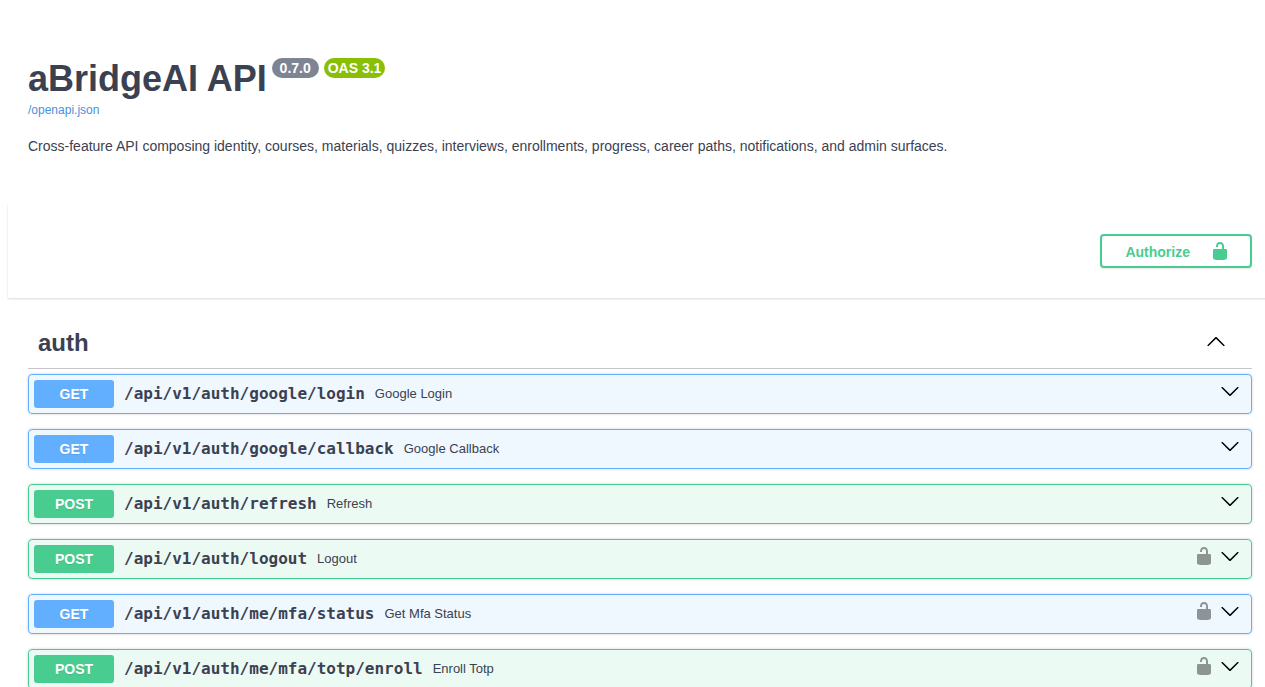
\includegraphics[width=0.92\textwidth,height=0.82\textheight,keepaspectratio]{graphics/swagger/00_overview.png}
    \caption{Live Swagger UI at \texttt{/docs} (rendered from the FastAPI \texttt{/openapi.json}): title, authorise control, and the \texttt{auth} audience-tag section.}
    \label{fig:swagger_overview_main}
\end{figure}

% ────────────────────────────────────────────────────
\subsection{Endpoint Catalogue}
% ────────────────────────────────────────────────────────────

The following tables enumerate every endpoint exposed by the backend, grouped by feature and audience. All paths are relative to \path|/api/v1|. The \textit{Auth} column reads ``Bearer'' when an authenticated session is required (the default), ``Public'' for anonymous endpoints, and ``Bearer + role'' when an additional role check applies.

% ── Identity ────────────────────────────────────────────────
\subsubsection{Identity --- Authentication \& Profile}

\begin{longtable}{|p{0.105\textwidth}|p{0.388\textwidth}|p{0.11\textwidth}|p{0.277\textwidth}|}
    \caption{Identity endpoints (Google OAuth, refresh, logout, profile).} \label{tab:api_identity} \\
    \hline
    \textbf{Method} & \textbf{Path} & \textbf{Auth} & \textbf{Description} \\
    \hline
    \endfirsthead
    \multicolumn{4}{c}{\small\tablename~\thetable{} \textit{(continued)}} \\
    \hline
    \textbf{Method} & \textbf{Path} & \textbf{Auth} & \textbf{Description} \\
    \hline
    \endhead
    \hline
    \endfoot
    GET    & \path|/auth/google/login|    & Public   & Return the Google OAuth authorisation URL plus an opaque \path|state|. \\ \hline
    GET    & \path|/auth/google/callback| & Public   & Exchange the Google authorisation code for an access/refresh pair. \\ \hline
    POST   & \path|/auth/refresh|         & Public$^\ast$ & Rotate the refresh token; returns a fresh token pair. \\ \hline
    POST   & \path|/auth/logout|          & Bearer   & Invalidate the current refresh-token row server-side. \\ \hline
    GET    & \path|/users/me|             & Bearer   & Return the authenticated user's profile. \\ \hline
    PATCH  & \path|/users/me/profile|     & Bearer   & Update display name, avatar, locale, etc. \\ \hline
    GET    & \path|/users/me/permissions| & Bearer   & Return effective roles and permission flags. \\ \hline
    GET    & \path|/users|                & Bearer   & Search users by name or email (auto-complete; admin-scoped). \\ \hline
    GET    & \path|/users/{user_id}|      & Bearer   & Return a public profile by ID. \\ \hline
\end{longtable}

\noindent$^\ast$\textit{The refresh token itself is the credential; no Bearer header is required.}

% ── Access control ──────────────────────────────────────────
\subsubsection{Access Control --- Roles, Grants \& Organisations}

\begin{longtable}{|p{0.105\textwidth}|p{0.425\textwidth}|p{0.11\textwidth}|p{0.24\textwidth}|}
    \caption{Access-control endpoints (admin-scoped).} \label{tab:api_access_control} \\
    \hline
    \textbf{Method} & \textbf{Path} & \textbf{Auth} & \textbf{Description} \\
    \hline
    \endfirsthead
    \multicolumn{4}{c}{\small\tablename~\thetable{} \textit{(continued)}} \\
    \hline
    \textbf{Method} & \textbf{Path} & \textbf{Auth} & \textbf{Description} \\
    \hline
    \endhead
    \hline
    \endfoot
    GET    & \path|/admin/permissions| & Bearer + admin & List the permission catalogue. \\ \hline
    GET    & \path|/admin/roles|       & Bearer + admin & List system and tenant roles with their permissions. \\ \hline
    GET    & \path|/admin/users/{user_id}/assignments|                          & Bearer + admin & List role assignments for a user. \\ \hline
    POST   & \path|/admin/users/{user_id}/assignments|                          & Bearer + admin & Assign a role to a user (optionally org-scoped). \\ \hline
    DELETE & \path|/admin/users/{user_id}/assignments/{assignment_id}|          & Bearer + admin & Revoke a role assignment. \\ \hline
    GET    & \path|/admin/users/{user_id}/grants|                               & Bearer + admin & List ad-hoc permission grants for a user. \\ \hline
    POST   & \path|/admin/users/{user_id}/grants|                               & Bearer + admin & Issue an ad-hoc permission grant. \\ \hline
    DELETE & \path|/admin/users/{user_id}/grants/{grant_id}|                    & Bearer + admin & Revoke an ad-hoc grant. \\ \hline
    GET    & \path|/admin/organizations|                                        & Bearer + admin & List tenant organisations. \\ \hline
    POST   & \path|/admin/organizations|                                        & Bearer + admin & Create a tenant organisation. \\ \hline
    GET    & \path|/admin/organizations/{org_id}|                               & Bearer + admin & Get an organisation. \\ \hline
    PATCH  & \path|/admin/organizations/{org_id}|                               & Bearer + admin & Update organisation settings. \\ \hline
    DELETE & \path|/admin/organizations/{org_id}|                               & Bearer + admin & Soft-delete an organisation. \\ \hline
    GET    & \path|/admin/organizations/{org_id}/domains|                       & Bearer + admin & List email domains owned by the organisation. \\ \hline
    POST   & \path|/admin/organizations/{org_id}/domains|                       & Bearer + admin & Add an owned email domain. \\ \hline
    PATCH  & \path|/admin/organization-domains/{domain_id}|                     & Bearer + admin & Update a domain (rename, mark verified). \\ \hline
    DELETE & \path|/admin/organization-domains/{domain_id}|                     & Bearer + admin & Remove an owned domain. \\ \hline
    GET    & \path|/admin/organizations/{org_id}/units|                         & Bearer + admin & List org units (faculties, departments). \\ \hline
    POST   & \path|/admin/organizations/{org_id}/units|                         & Bearer + admin & Create an org unit. \\ \hline
    GET    & \path|/admin/org-units/{unit_id}|                                  & Bearer + admin & Get an org unit. \\ \hline
    PATCH  & \path|/admin/org-units/{unit_id}|                                  & Bearer + admin & Update an org unit. \\ \hline
    DELETE & \path|/admin/org-units/{unit_id}|                                  & Bearer + admin & Delete an org unit. \\ \hline
    GET    & \path|/admin/organizations/{org_id}/memberships|                   & Bearer + admin & List user memberships in an organisation. \\ \hline
    POST   & \path|/admin/organizations/{org_id}/memberships|                   & Bearer + admin & Add a user to an organisation. \\ \hline
    PATCH  & \path|/admin/organization-memberships/{membership_id}|             & Bearer + admin & Update membership status. \\ \hline
    DELETE & \path|/admin/organization-memberships/{membership_id}|             & Bearer + admin & Remove a membership. \\ \hline
\end{longtable}

% ── Courses (learner) ───────────────────────────────────────
\subsubsection{Courses --- Learner}

\begin{longtable}{|p{0.105\textwidth}|p{0.425\textwidth}|p{0.11\textwidth}|p{0.24\textwidth}|}
    \caption{Course-learner endpoints (the calling user's own enrolments).} \label{tab:api_courses_learner} \\
    \hline
    \textbf{Method} & \textbf{Path} & \textbf{Auth} & \textbf{Description} \\
    \hline
    \endfirsthead
    \multicolumn{4}{c}{\small\tablename~\thetable{} \textit{(continued)}} \\
    \hline
    \textbf{Method} & \textbf{Path} & \textbf{Auth} & \textbf{Description} \\
    \hline
    \endhead
    \hline
    \endfoot
    GET    & \path|/me/courses/courses|                                                & Bearer & List the caller's enrolled courses. \\ \hline
    GET    & \path|/me/courses/courses/by-slug/{slug}|                                  & Bearer & Resolve a course by its public slug. \\ \hline
    GET    & \path|/me/courses/courses/{course_id}|                                     & Bearer & Get course detail. \\ \hline
    GET    & \path|/me/courses/courses/{course_id}/content|                             & Bearer & Get the full module/lesson tree. \\ \hline
    GET    & \path|/me/courses/courses/{course_id}/tags|                                & Bearer & Get the course's tags. \\ \hline
    GET    & \path|/me/courses/courses/{course_id}/outcomes|                            & Bearer & Get the course's learning outcomes. \\ \hline
    GET    & \path|/me/courses/courses/{course_id}/modules|                             & Bearer & List modules with publish state. \\ \hline
    GET    & \path|/me/courses/modules/{module_id}|                                     & Bearer & Get a module. \\ \hline
    GET    & \path|/me/courses/modules/{module_id}/items|                               & Bearer & List ordered lesson/quiz items. \\ \hline
    GET    & \path|/me/courses/modules/{module_id}/lessons|                             & Bearer & List lessons in a module. \\ \hline
    GET    & \path|/me/courses/lessons/{lesson_id}|                                     & Bearer & Get a lesson. \\ \hline
    GET    & \path|/me/courses/lessons/{lesson_id}/resources|                           & Bearer & List downloadable lesson resources. \\ \hline
    GET    & \path|/me/courses/lesson-resources/{resource_id}/download-url|             & Bearer & Issue a presigned S3 URL for a resource. \\ \hline
\end{longtable}

% ── Courses (authoring / dept / admin) ──────────────────────
\subsubsection{Courses --- Authoring (Teacher)}

\begin{longtable}{|p{0.1\textwidth}|p{0.424\textwidth}|p{0.15\textwidth}|p{0.206\textwidth}|}
    \caption{Course-authoring endpoints (teacher role).} \label{tab:api_courses_authoring} \\
    \hline
    \textbf{Method} & \textbf{Path} & \textbf{Auth} & \textbf{Description} \\
    \hline
    \endfirsthead
    \multicolumn{4}{c}{\small\tablename~\thetable{} \textit{(continued)}} \\
    \hline
    \textbf{Method} & \textbf{Path} & \textbf{Auth} & \textbf{Description} \\
    \hline
    \endhead
    \hline
    \endfoot
    POST   & \path|/teacher/courses|                                            & Bearer + manager & Create a course. Requires \path|course.create|, which a teacher does not hold. \\ \hline
    GET    & \path|/teacher/courses/check-slug|                                 & Bearer + manager & Probe slug availability; pre-flight for the create form, so same permission. \\ \hline
    GET    & \path|/teacher/courses|                                            & Bearer + teacher & List courses owned or co-taught by the caller. \\ \hline
    GET    & \path|/teacher/courses/{course_id}|                                & Bearer + teacher & Get a course (authoring view). \\ \hline
    GET    & \path|/teacher/courses/{course_id}/content|                        & Bearer + teacher & Get the full module/lesson/quiz tree. \\ \hline
    GET    & \path|/teacher/courses/{course_id}/roster|                         & Bearer + teacher & List enrolled students. \\ \hline
    PATCH  & \path|/teacher/courses/{course_id}|                                & Bearer + teacher & Update course metadata. \\ \hline
    POST   & \path|/teacher/courses/{course_id}/publish|                        & Bearer + teacher & Publish the course. \\ \hline
    POST   & \path|/teacher/courses/{course_id}/archive|                        & Bearer + teacher & Archive the course. \\ \hline
    POST   & \path|/teacher/courses/{course_id}/modules|                        & Bearer + teacher & Add a module. \\ \hline
    PATCH  & \path|/teacher/modules/{module_id}|                                & Bearer + teacher & Update a module. \\ \hline
    PUT    & \path|/teacher/modules/{module_id}/prerequisites|                  & Bearer + teacher & Set module prerequisites. \\ \hline
    PUT    & \path|/teacher/modules/{module_id}/items/reorder|                  & Bearer + teacher & Reorder module items (drag-and-drop). \\ \hline
    PATCH  & \path|/teacher/module-items/{module_item_id}|                      & Bearer + teacher & Update a module-item entry. \\ \hline
    DELETE & \path|/teacher/module-items/{module_item_id}|                      & Bearer + teacher & Remove a module-item entry. \\ \hline
    GET    & \path|/teacher/modules/{module_id}/lessons|                        & Bearer + teacher & List lessons within a module. \\ \hline
    POST   & \path|/teacher/modules/{module_id}/lessons|                        & Bearer + teacher & Create a lesson. \\ \hline
    GET    & \path|/teacher/lessons/{lesson_id}|                                & Bearer + teacher & Get a lesson. \\ \hline
    GET    & \path|/teacher/lessons/{lesson_id}/outline|                        & Bearer + teacher & Get the structural outline of the lesson. \\ \hline
    GET    & \path|/teacher/lessons/{lesson_id}/resources|                      & Bearer + teacher & List downloadable resources. \\ \hline
    PATCH  & \path|/teacher/lessons/{lesson_id}|                                & Bearer + teacher & Update a lesson. \\ \hline
    POST   & \path|/teacher/lessons/{lesson_id}/resources|                      & Bearer + teacher & Attach a resource. \\ \hline
    DELETE & \path|/teacher/lesson-resources/{resource_id}|                     & Bearer + teacher & Detach a resource. \\ \hline
    GET    & \path|/teacher/lesson-resources/{resource_id}/download-url|        & Bearer + teacher & Issue a presigned download URL. \\ \hline
\end{longtable}

\subsubsection{Courses --- Department \& Administration}

\begin{longtable}{|p{0.1\textwidth}|p{0.424\textwidth}|p{0.15\textwidth}|p{0.206\textwidth}|}
    \caption{Course department-assignment and administration endpoints.} \label{tab:api_courses_dept_admin} \\
    \hline
    \textbf{Method} & \textbf{Path} & \textbf{Auth} & \textbf{Description} \\
    \hline
    \endfirsthead
    \multicolumn{4}{c}{\small\tablename~\thetable{} \textit{(continued)}} \\
    \hline
    \textbf{Method} & \textbf{Path} & \textbf{Auth} & \textbf{Description} \\
    \hline
    \endhead
    \hline
    \endfoot
    GET    & \path|/dept/courses|                                       & Bearer + dept   & List courses for the caller's department. \\ \hline
    GET    & \path|/dept/courses/{course_id}/teachers|                  & Bearer + dept   & List teachers assigned to a course. \\ \hline
    POST   & \path|/dept/courses/{course_id}/teachers|                  & Bearer + dept   & Assign a teacher to a course. \\ \hline
    DELETE & \path|/dept/courses/{course_id}/teachers/{user_id}|        & Bearer + dept   & Unassign a teacher. \\ \hline
    GET    & \path|/dept/courses/{course_id}/roster|                    & Bearer + dept   & Read the enrolled-student roster. \\ \hline
    GET    & \path|/dept/org-units/{org_unit_id}/courses|               & Bearer + dept   & List courses owned by an org unit. \\ \hline
    GET    & \path|/admin/courses|                                      & Bearer + admin  & Cross-organisation course listing. \\ \hline
    POST   & \path|/admin/courses/{course_id}/restore|                  & Bearer + admin  & Restore a soft-deleted course. \\ \hline
    GET    & \path|/admin/courses/{course_id}/audit|                    & Bearer + admin  & Course-level audit trail. \\ \hline
    GET    & \path|/admin/courses/{course_id}/processing|               & Bearer + admin  & Per-course AI processing history. \\ \hline
    GET    & \path|/admin/courses/_stats|                               & Bearer + admin  & Cross-org course aggregates. \\ \hline
\end{longtable}

% ── Materials ───────────────────────────────────────────────
\subsubsection{Materials}

Material upload uses a two-phase protocol so large files can be streamed directly from the browser to the object store (Garage S3-compatible) without traversing the application server. The teacher first calls \path|init-upload| to receive a presigned URL or a multipart upload ID; the SPA then uploads the bytes; finally it calls \path|complete| (or \path|.../multipart/complete|) to register the version and trigger AI processing.

\begin{longtable}{|p{0.1\textwidth}|p{0.461\textwidth}|p{0.15\textwidth}|p{0.169\textwidth}|}
    \caption{Materials endpoints.} \label{tab:api_materials} \\
    \hline
    \textbf{Method} & \textbf{Path} & \textbf{Auth} & \textbf{Description} \\
    \hline
    \endfirsthead
    \multicolumn{4}{c}{\small\tablename~\thetable{} \textit{(continued)}} \\
    \hline
    \textbf{Method} & \textbf{Path} & \textbf{Auth} & \textbf{Description} \\
    \hline
    \endhead
    \hline
    \endfoot
    POST   & \path|/teacher/lessons/{lesson_id}/materials/init-upload|                                 & Bearer + teacher & Begin an upload (single-part or multipart). \\ \hline
    POST   & \path|/teacher/materials/{material_id}/versions/{version_id}/multipart/parts|             & Bearer + teacher & Issue per-part presigned URLs. \\ \hline
    POST   & \path|/teacher/materials/{material_id}/versions/{version_id}/multipart/complete|          & Bearer + teacher & Finalise a multipart upload. \\ \hline
    POST   & \path|/teacher/materials/{material_id}/versions/{version_id}/multipart/abort|             & Bearer + teacher & Abort a multipart upload. \\ \hline
    POST   & \path|/teacher/materials/{material_id}/versions/{version_id}/complete|                    & Bearer + teacher & Finalise a single-part upload and queue processing. \\ \hline
    GET    & \path|/teacher/lessons/{lesson_id}/materials|                                             & Bearer + teacher & List materials attached to a lesson. \\ \hline
    POST   & \path|/teacher/lessons/{lesson_id}/materials/link|                                        & Bearer + teacher & Link an existing material into another lesson. \\ \hline
    GET    & \path|/teacher/lessons/{lesson_id}/processing-summary|                                    & Bearer + teacher & Aggregate AI-processing state for a lesson. \\ \hline
    GET    & \path|/teacher/materials/{material_id}|                                                   & Bearer + teacher & Get material detail. \\ \hline
    GET    & \path|/teacher/materials/{material_id}/processing-summary|                                & Bearer + teacher & Per-material processing state. \\ \hline
    GET    & \path|/teacher/materials/{material_id}/stream-url|                                        & Bearer + teacher & Issue a presigned streaming URL (PDF/video). \\ \hline
    PATCH  & \path|/teacher/materials/{material_id}|                                                   & Bearer + teacher & Update material metadata. \\ \hline
    POST   & \path|/teacher/materials/{material_id}/reprocess|                                         & Bearer + teacher & Re-run AI ingestion on the latest version. \\ \hline
    DELETE & \path|/teacher/materials/{material_id}|                                                   & Bearer + teacher & Soft-delete a material. \\ \hline
    GET    & \path|/materials/{material_id}|                                                           & Bearer & Learner-facing material descriptor. \\ \hline
    GET    & \path|/materials/{material_id}/stream-url|                                                & Bearer & Learner-facing presigned streaming URL. \\ \hline
    GET    & \path|/materials/{material_id}/chunks/preview|                                            & Bearer & Preview the first N text chunks for review. \\ \hline
\end{longtable}

% ── Quizzes ─────────────────────────────────────────────────
\subsubsection{Quizzes}

Quiz authoring follows a draft / generate / review / publish pipeline. \path|POST .../quizzes/{quiz_id}/generate| accepts a generation spec (source lessons, count, mode, types) and returns a \path|run_id| immediately; the SPA polls \path|.../generation-runs/{run_id}| to surface progress. Generated questions land in a \textit{Pending Review} state and are visible to students only after explicit instructor approval.

\begin{longtable}{|p{0.1\textwidth}|p{0.461\textwidth}|p{0.15\textwidth}|p{0.169\textwidth}|}
    \caption{Quizzes endpoints.} \label{tab:api_quizzes} \\
    \hline
    \textbf{Method} & \textbf{Path} & \textbf{Auth} & \textbf{Description} \\
    \hline
    \endfirsthead
    \multicolumn{4}{c}{\small\tablename~\thetable{} \textit{(continued)}} \\
    \hline
    \textbf{Method} & \textbf{Path} & \textbf{Auth} & \textbf{Description} \\
    \hline
    \endhead
    \hline
    \endfoot
    POST   & \path|/teacher/courses/{course_id}/quizzes|                                       & Bearer + teacher & Create a quiz on a module. \\ \hline
    GET    & \path|/teacher/quizzes/{quiz_id}|                                                  & Bearer + teacher & Get authoring view of a quiz. \\ \hline
    PATCH  & \path|/teacher/quizzes/{quiz_id}|                                                  & Bearer + teacher & Update quiz metadata. \\ \hline
    POST   & \path|/teacher/quizzes/{quiz_id}/publish|                                          & Bearer + teacher & Publish the quiz. \\ \hline
    POST   & \path|/teacher/quizzes/{quiz_id}/questions/bulk-set-expected-time|                 & Bearer + teacher & Apply a uniform per-question time. \\ \hline
    DELETE & \path|/teacher/quizzes/{quiz_id}|                                                  & Bearer + teacher & Delete a quiz. \\ \hline
    POST   & \path|/teacher/quizzes/{quiz_id}/generate|                                         & Bearer + teacher & Queue an AI generation run; returns \path|run_id|. \\ \hline
    GET    & \path|/teacher/quizzes/{quiz_id}/generation-runs/latest|                           & Bearer + teacher & Latest generation-run status. \\ \hline
    GET    & \path|/teacher/quizzes/{quiz_id}/generation-runs/{run_id}|                         & Bearer + teacher & Specific run status. \\ \hline
    POST   & \path|/teacher/quizzes/{quiz_id}/questions|                                        & Bearer + teacher & Add a question manually. \\ \hline
    PATCH  & \path|/teacher/quizzes/{quiz_id}/questions/{question_id}|                          & Bearer + teacher & Update or approve a question. \\ \hline
    DELETE & \path|/teacher/quizzes/{quiz_id}/questions/{question_id}|                          & Bearer + teacher & Delete a question. \\ \hline
    POST   & \path|/teacher/quizzes/{quiz_id}/questions/{question_id}/regenerate|               & Bearer + teacher & Regenerate a single AI question. \\ \hline
    GET    & \path|/teacher/courses/{course_id}/question-bank|                                  & Bearer + teacher & Browse the course-level question bank. \\ \hline
    POST   & \path|/teacher/quizzes/{quiz_id}/questions/import|                                 & Bearer + teacher & Import from the question bank. \\ \hline
    GET    & \path|/quizzes/{quiz_id}|                                                          & Bearer & Learner view (questions only, no answers). \\ \hline
    POST   & \path|/quizzes/{quiz_id}/attempts|                                                 & Bearer & Start a new attempt. \\ \hline
    POST   & \path|/attempts/{attempt_id}/answers|                                              & Bearer & Submit one or more answers. \\ \hline
    POST   & \path|/attempts/{attempt_id}/submit|                                               & Bearer & Finalise the attempt; trigger scoring. \\ \hline
    GET    & \path|/attempts/{attempt_id}|                                                      & Bearer & Attempt detail. \\ \hline
    GET    & \path|/attempts/{attempt_id}/review|                                               & Bearer & Per-question review with correct answers. \\ \hline
    POST   & \path|/attempts/{attempt_id}/session/claim|                                        & Bearer & Claim single-client ownership of a live attempt. \\ \hline
    POST   & \path|/attempts/{attempt_id}/session/heartbeat|                                    & Bearer & Renew ownership while the attempt is open. \\ \hline
    POST   & \path|/attempts/{attempt_id}/session/takeover|                                     & Bearer & Transfer ownership to this client on explicit confirmation. \\ \hline
    POST   & \path|/attempts/{attempt_id}/session/release|                                      & Bearer & Release ownership; the attempt stays resumable. \\ \hline
    GET    & \path|/me/quizzes/{quiz_id}/attempts|                                              & Bearer & Caller's attempt history for the quiz. \\ \hline
\end{longtable}

% ── Interviews ──────────────────────────────────────────────
\subsubsection{Interviews}

\begin{longtable}{|p{0.1\textwidth}|p{0.461\textwidth}|p{0.15\textwidth}|p{0.169\textwidth}|}
    \caption{Interview endpoints (AI mock-interview surface).} \label{tab:api_interviews} \\
    \hline
    \textbf{Method} & \textbf{Path} & \textbf{Auth} & \textbf{Description} \\
    \hline
    \endfirsthead
    \multicolumn{4}{c}{\small\tablename~\thetable{} \textit{(continued)}} \\
    \hline
    \textbf{Method} & \textbf{Path} & \textbf{Auth} & \textbf{Description} \\
    \hline
    \endhead
    \hline
    \endfoot
    POST   & \path|/teacher/courses/{course_id}/interview-configs|                                & Bearer + teacher & Create an interview configuration. \\ \hline
    GET    & \path|/teacher/interview-configs/{config_id}|                                          & Bearer + teacher & Get a configuration. \\ \hline
    PATCH  & \path|/teacher/interview-configs/{config_id}|                                          & Bearer + teacher & Update a configuration. \\ \hline
    POST   & \path|/teacher/interview-configs/{config_id}/publish|                                  & Bearer + teacher & Publish the configuration. \\ \hline
    DELETE & \path|/teacher/interview-configs/{config_id}|                                          & Bearer + teacher & Delete a configuration. \\ \hline
    POST   & \path|/teacher/interview-configs/{config_id}/generate|                                 & Bearer + teacher & Queue AI question generation. \\ \hline
    GET    & \path|/teacher/interview-configs/{config_id}/generation-runs/{run_id}|                 & Bearer + teacher & Generation-run status. \\ \hline
    POST   & \path|/teacher/interview-configs/{config_id}/questions|                                & Bearer + teacher & Add a question manually. \\ \hline
    PATCH  & \path|/teacher/interview-configs/{config_id}/questions/{question_id}|                  & Bearer + teacher & Update or approve a question. \\ \hline
    DELETE & \path|/teacher/interview-configs/{config_id}/questions/{question_id}|                  & Bearer + teacher & Delete a question. \\ \hline
    POST   & \path|/teacher/interview-configs/{config_id}/questions/{question_id}/regenerate|       & Bearer + teacher & Regenerate a single question. \\ \hline
    POST   & \path|/teacher/interview-configs/{config_id}/outcomes|                                 & Bearer + teacher & Add a desired outcome. \\ \hline
    PATCH  & \path|/teacher/interview-configs/{config_id}/outcomes/{outcome_id}|                    & Bearer + teacher & Update an outcome. \\ \hline
    GET    & \path|/teacher/interview-sessions/{session_id}/gap-report|                             & Bearer + teacher & Per-student gap report (instructor view). \\ \hline
    GET    & \path|/teacher/interview-sessions/{session_id}/recording|                              & Bearer + teacher & Short-lived playback URL or recording availability state; consent alone does not guarantee media exists. \\ \hline
    GET    & \path|/interview-configs/{config_id}|                                                  & Bearer & Learner-facing config view. \\ \hline
    POST   & \path|/interview-configs/{config_id}/sessions|                                         & Bearer & Start or resume an interview session. \\ \hline
    GET    & \path|/interview-sessions/{session_id}|                                                & Bearer & Get session state and persisted history. \\ \hline
    POST   & \path|/interview-sessions/{session_id}/onboarding/respond|                             & Bearer & Persist one onboarding step before assessed questioning. \\ \hline
    POST   & \path|/interview-sessions/{session_id}/realtime-token|                                 & Bearer & Mint a room participant token; \texttt{warm=true} joins without agent dispatch. \\ \hline
    POST   & \path|/interview-sessions/{session_id}/realtime-agent|                                 & Bearer & Dispatch the native LiveKit agent after readiness. \\ \hline
    POST   & \path|/interview-sessions/{session_id}/recording-consent|                              & Bearer & Record or revoke versioned audio-recording consent. \\ \hline
    POST   & \path|/interview-sessions/{session_id}/integrity-events|                               & Bearer & Batch browser integrity signals for server-side review. \\ \hline
    POST   & \path|/interview-sessions/{session_id}/narration|                                      & Bearer & Request controlled server-side narration where applicable. \\ \hline
    POST   & \path|/interview-sessions/{session_id}/respond|                                        & Bearer & REST/routed compatibility turn endpoint using \texttt{take\_session\_step}; native room turns use LiveKit. \\ \hline
    POST   & \path|/interview-sessions/{session_id}/finish|                                         & Bearer & Finalise the session; trigger AI scoring. \\ \hline
    GET    & \path|/interview-sessions/{session_id}/gap-report|                                     & Bearer & Per-student gap report (learner view). \\ \hline
    GET    & \path|/me/interview-sessions|                                                          & Bearer & Caller's interview-session history. \\ \hline
\end{longtable}

% ── Progress ────────────────────────────────────────────────
\subsubsection{Progress}

\begin{longtable}{|p{0.1\textwidth}|p{0.461\textwidth}|p{0.15\textwidth}|p{0.169\textwidth}|}
    \caption{Progress endpoints.} \label{tab:api_progress} \\
    \hline
    \textbf{Method} & \textbf{Path} & \textbf{Auth} & \textbf{Description} \\
    \hline
    \endfirsthead
    \multicolumn{4}{c}{\small\tablename~\thetable{} \textit{(continued)}} \\
    \hline
    \textbf{Method} & \textbf{Path} & \textbf{Auth} & \textbf{Description} \\
    \hline
    \endhead
    \hline
    \endfoot
    GET    & \path|/me/progress/lessons/{lesson_id}|              & Bearer & Caller's progress for a lesson. \\ \hline
    GET    & \path|/me/progress/courses/{course_id}|              & Bearer & Caller's progress for a course. \\ \hline
    POST   & \path|/me/progress/material-engagement|              & Bearer & Record a material-engagement event (heartbeat). \\ \hline
    POST   & \path|/me/progress/lessons/{lesson_id}/complete|     & Bearer & Mark a lesson complete. \\ \hline
    POST   & \path|/me/progress/lessons/{lesson_id}/uncomplete|   & Bearer & Undo lesson completion. \\ \hline
    GET    & \path|/teacher/courses/{course_id}/progress/roster|  & Bearer + teacher & Per-student progress roster for a course. \\ \hline
    GET    & \path|/teacher/courses/{course_id}/progress/at-risk| & Bearer + teacher & At-risk student list (low completion / quiz score). \\ \hline
\end{longtable}

% ── Career paths ────────────────────────────────────────────
\subsubsection{Career Paths --- Learner}

\begin{longtable}{|p{0.1\textwidth}|p{0.424\textwidth}|p{0.15\textwidth}|p{0.206\textwidth}|}
    \caption{Career-path endpoints --- learner catalogue and enrolment.} \label{tab:api_career_paths} \\
    \hline
    \textbf{Method} & \textbf{Path} & \textbf{Auth} & \textbf{Description} \\
    \hline
    \endfirsthead
    \multicolumn{4}{c}{\small\tablename~\thetable{} \textit{(continued)}} \\
    \hline
    \textbf{Method} & \textbf{Path} & \textbf{Auth} & \textbf{Description} \\
    \hline
    \endhead
    \hline
    \endfoot
    GET    & \path|/career-paths|                                                    & Bearer & List published career paths, scoped to those the caller's programme offers. \\ \hline
    GET    & \path|/career-paths/{slug}|                                             & Bearer & Career-path detail with its ordered course list. \\ \hline
    GET    & \path|/career-paths/{slug}/detail|                                      & Bearer & The same path plus its stage roadmap. \\ \hline
    GET    & \path|/me/career-enrollments|                                           & Bearer & The caller's pathway enrolments with derived progress. \\ \hline
    GET    & \path|/me/career-enrollments/{career_path_id}/progress|                 & Bearer & Stage-aware progress against the pinned version (Section~\ref{sec:pathway_completion}). \\ \hline
    GET    & \path|/me/career-enrollments/{career_path_id}/readiness-history|        & Bearer & Readiness snapshots, most recent first (FR-6.8). \\ \hline
    POST   & \path|/me/career-enrollments/{career_path_id}/courses/{course_id}/start| & Bearer & Start one course of a pathway the caller already holds. \\ \hline
\end{longtable}

\subsubsection{Career Paths --- Authoring \& Roster}

\begin{longtable}{|p{0.1\textwidth}|p{0.424\textwidth}|p{0.15\textwidth}|p{0.206\textwidth}|}
    \caption{Career-path endpoints --- authoring, publication and roster.} \label{tab:api_career_paths_authoring} \\
    \hline
    \textbf{Method} & \textbf{Path} & \textbf{Auth} & \textbf{Description} \\
    \hline
    \endfirsthead
    \multicolumn{4}{c}{\small\tablename~\thetable{} \textit{(continued)}} \\
    \hline
    \textbf{Method} & \textbf{Path} & \textbf{Auth} & \textbf{Description} \\
    \hline
    \endhead
    \hline
    \endfoot
    POST   & \path|/management/career-paths|                                              & Bearer + manager & Create a pathway as a draft. \\ \hline
    GET    & \path|/management/career-paths|                                              & Bearer + manager & List the organisation's pathways. \\ \hline
    GET    & \path|/management/career-paths/{career_path_id}|                              & Bearer + manager & Pathway detail for authoring. \\ \hline
    PATCH  & \path|/management/career-paths/{career_path_id}|                              & Bearer + manager & Edit pathway metadata. \\ \hline
    PUT    & \path|/management/career-paths/{career_path_id}/thumbnail|                    & Bearer + manager & Upload a JPEG/PNG/WebP/GIF thumbnail, up to 5~MiB. \\ \hline
    GET    & \path|/management/career-paths/{career_path_id}/impact|                       & Bearer + manager & Blast radius of an edit: who is enrolled and what would move. \\ \hline
    GET    & \path|/management/career-paths/{career_path_id}/versions|                     & Bearer + manager & Version history, newest first; a published version is frozen. \\ \hline
    POST   & \path|/management/career-paths/{career_path_id}/versions|                     & Bearer + manager & Fork the latest published version into a new draft. \\ \hline
    GET    & \path|/management/career-paths/{career_path_id}/courses|                      & Bearer + manager & Courses attached to the working version. \\ \hline
    POST   & \path|/management/career-paths/{career_path_id}/courses|                      & Bearer + manager & Attach a course to the pathway. \\ \hline
    PATCH  & \path|/management/career-paths/{career_path_id}/courses/{course_id}|          & Bearer + manager & Edit an attached course's required / satisfied-by flags. \\ \hline
    DELETE & \path|/management/career-paths/{career_path_id}/courses/{course_id}|          & Bearer + manager & Detach a course. \\ \hline
    PUT    & \path|/management/career-paths/{career_path_id}/courses/reorder|              & Bearer + manager & Reorder courses within the pathway. \\ \hline
    PUT    & \path|/management/career-paths/{career_path_id}/courses/{course_id}/stage|    & Bearer + manager & Move a course between stages, or reposition it within one. \\ \hline
    GET    & \path|/management/career-paths/{career_path_id}/course-candidates|            & Bearer + manager & Organisation course catalogue for the attach picker, any status. \\ \hline
    GET    & \path|/management/career-paths/{career_path_id}/stages|                       & Bearer + manager & Stages of the working version. \\ \hline
    POST   & \path|/management/career-paths/{career_path_id}/stages|                       & Bearer + manager & Create a stage; an empty stage is valid. \\ \hline
    PATCH  & \path|/management/career-paths/{career_path_id}/stages/{stage_id}|            & Bearer + manager & Edit a stage's title, unlock policy or elective quota. \\ \hline
    DELETE & \path|/management/career-paths/{career_path_id}/stages/{stage_id}|            & Bearer + manager & Delete a stage; refused while it holds courses. \\ \hline
    PUT    & \path|/management/career-paths/{career_path_id}/stages/reorder|               & Bearer + manager & Reorder stages; returns warnings rather than rewriting unlock policy. \\ \hline
    POST   & \path|/management/career-paths/{career_path_id}/students|                     & Bearer + manager & Assign students to the pathway. \\ \hline
    DELETE & \path|/management/career-paths/{career_path_id}/students/{student_id}|        & Bearer + manager & Withdraw a student from the pathway. \\ \hline
    POST   & \path|/management/career-paths/{career_path_id}/publish|                      & Bearer + manager & Publish, freezing the version after the completeness gate. \\ \hline
    POST   & \path|/management/career-paths/{career_path_id}/archive|                      & Bearer + manager & Archive; blocks new selections without interrupting current ones. \\ \hline
    GET    & \path|/management/career-paths/{career_path_id}/readiness|                    & Bearer + manager & Readiness aggregate over actively-enrolled students (FR-6.8). \\ \hline
    GET    & \path|/teacher/career-paths/{career_path_id}/students/progress|               & Bearer + teacher & Per-student roster progress, derived from the stage evaluation. \\ \hline
\end{longtable}

% ── Spaced repetition ───────────────────────────────────────
\subsubsection{Spaced Repetition}

\begin{longtable}{|p{0.1\textwidth}|p{0.461\textwidth}|p{0.15\textwidth}|p{0.169\textwidth}|}
    \caption{Spaced-repetition endpoints (hybrid SM-2 scheduler).} \label{tab:api_sr} \\
    \hline
    \textbf{Method} & \textbf{Path} & \textbf{Auth} & \textbf{Description} \\
    \hline
    \endfirsthead
    \multicolumn{4}{c}{\small\tablename~\thetable{} \textit{(continued)}} \\
    \hline
    \textbf{Method} & \textbf{Path} & \textbf{Auth} & \textbf{Description} \\
    \hline
    \endhead
    \hline
    \endfoot
    GET    & \path|/me/cards-due|                                                                & Bearer & Cards due for review across all courses. \\ \hline
    GET    & \path|/me/lessons/{lesson_id}/sr-summary|                                           & Bearer & Per-lesson SR summary (retention, due count). \\ \hline
    GET    & \path|/me/courses/{course_id}/sr-overview|                                          & Bearer & Per-course SR overview. \\ \hline
    GET    & \path|/teacher/courses/{course_id}/lessons/{lesson_id}/cohort-kr|                   & Bearer + teacher & Cohort-level retention distribution for a lesson. \\ \hline
    GET    & \path|/teacher/courses/{course_id}/lessons/{lesson_id}/difficult-cards|             & Bearer + teacher & Cards the cohort is struggling with. \\ \hline
    GET    & \path|/teacher/courses/{course_id}/at-risk|                                         & Bearer + teacher & Students flagged by SR signals. \\ \hline
    GET    & \path|/teacher/courses/{course_id}/students/{student_id}/sr-detail|                 & Bearer + teacher & A specific student's per-card SR data. \\ \hline
\end{longtable}

% ── Notifications ───────────────────────────────────────────
\subsubsection{Notifications}

\begin{longtable}{|p{0.1\textwidth}|p{0.461\textwidth}|p{0.15\textwidth}|p{0.169\textwidth}|}
    \caption{Notification endpoints.} \label{tab:api_notifications} \\
    \hline
    \textbf{Method} & \textbf{Path} & \textbf{Auth} & \textbf{Description} \\
    \hline
    \endfirsthead
    \multicolumn{4}{c}{\small\tablename~\thetable{} \textit{(continued)}} \\
    \hline
    \textbf{Method} & \textbf{Path} & \textbf{Auth} & \textbf{Description} \\
    \hline
    \endhead
    \hline
    \endfoot
    GET    & \path|/me/notifications|                                                & Bearer & List the caller's notifications. \\ \hline
    GET    & \path|/me/notifications/unread-count|                                   & Bearer & Unread-count badge. \\ \hline
    PATCH  & \path|/me/notifications/{notification_id}/read|                         & Bearer & Mark one notification read. \\ \hline
    POST   & \path|/me/notifications/mark-all-read|                                  & Bearer & Mark every notification read. \\ \hline
    DELETE & \path|/me/notifications/{notification_id}|                              & Bearer & Delete a notification. \\ \hline
    GET    & \path|/me/notification-preferences|                                     & Bearer & Read per-category, per-channel preferences. \\ \hline
    PATCH  & \path|/me/notification-preferences/{category}/{channel}|                & Bearer & Update one preference cell. \\ \hline
\end{longtable}

% ── Admin ───────────────────────────────────────────────────
\subsubsection{Admin Operations}

\begin{longtable}{|p{0.1\textwidth}|p{0.424\textwidth}|p{0.15\textwidth}|p{0.206\textwidth}|}
    \caption{Admin operations endpoints.} \label{tab:api_admin} \\
    \hline
    \textbf{Method} & \textbf{Path} & \textbf{Auth} & \textbf{Description} \\
    \hline
    \endfirsthead
    \multicolumn{4}{c}{\small\tablename~\thetable{} \textit{(continued)}} \\
    \hline
    \textbf{Method} & \textbf{Path} & \textbf{Auth} & \textbf{Description} \\
    \hline
    \endhead
    \hline
    \endfoot
    GET    & \path|/admin/stats/overview|       & Bearer + admin & Platform-level overview KPIs. \\ \hline
    GET    & \path|/admin/stats/active-users|   & Bearer + admin & Active-user time series. \\ \hline
    GET    & \path|/admin/stats/content|        & Bearer + admin & Content-volume metrics. \\ \hline
    GET    & \path|/admin/stats/health|         & Bearer + admin & Aggregated infrastructure-health probes. \\ \hline
    GET    & \path|/admin/users|                & Bearer + admin & Cross-org user listing with filters. \\ \hline
    GET    & \path|/admin/users/{user_id}|      & Bearer + admin & Get a user (admin view). \\ \hline
    POST   & \path|/admin/users/{user_id}/disable| & Bearer + admin & Disable an account. \\ \hline
    POST   & \path|/admin/users/{user_id}/enable|  & Bearer + admin & Re-enable an account. \\ \hline
    GET    & \path|/admin/processing/queue|        & Bearer + admin & Live ARQ queue depth and worker state. \\ \hline
    GET    & \path|/admin/processing/jobs|         & Bearer + admin & Recent AI background jobs. \\ \hline
    GET    & \path|/admin/processing/jobs/{job_id}| & Bearer + admin & Job detail and per-step log. \\ \hline
    POST   & \path|/admin/processing/jobs/{job_id}/retry| & Bearer + admin & Re-enqueue a failed job. \\ \hline
    GET    & \path|/admin/ai/costs/summary|        & Bearer + admin & Period-bounded cost summary. \\ \hline
    GET    & \path|/admin/ai/costs/by-user|        & Bearer + admin & Cost breakdown by user. \\ \hline
    GET    & \path|/admin/ai/costs/by-pipeline|    & Bearer + admin & Cost breakdown by pipeline stage. \\ \hline
    GET    & \path|/admin/ai/costs/recent|         & Bearer + admin & Recent cost events. \\ \hline
    GET    & \path|/admin/audit/role-changes|      & Bearer + admin & Role-change audit. \\ \hline
    GET    & \path|/admin/audit/data-changes|      & Bearer + admin & Data-change audit (DB triggers). \\ \hline
    GET    & \path|/admin/audit/http|              & Bearer + admin & HTTP-request audit log. \\ \hline
\end{longtable}

% ── Health ──────────────────────────────────────────────────
\subsubsection{Health}

The application mounts the health router both at the root (\path|/healthz|) for K8s liveness/readiness probes and under \path|/api/v1/healthz| so the SPA can probe through the same reverse-proxy path it uses for API traffic.

\begin{longtable}{|p{0.1\textwidth}|p{0.275\textwidth}|p{0.147\textwidth}|p{0.358\textwidth}|}
    \caption{Health-check endpoints.} \label{tab:api_health} \\
    \hline
    \textbf{Method} & \textbf{Path} & \textbf{Auth} & \textbf{Description} \\
    \hline
    \endfirsthead
    \multicolumn{4}{c}{\small\tablename~\thetable{} \textit{(continued)}} \\
    \hline
    \textbf{Method} & \textbf{Path} & \textbf{Auth} & \textbf{Description} \\
    \hline
    \endhead
    \hline
    \endfoot
    GET & \path|/healthz|       & Public & Liveness probe; returns 200 if the process is up. \\ \hline
    GET & \path|/healthz/deep|  & Public & Deep probe; checks DB and Redis connectivity. \\ \hline
    GET & \path|/readyz|        & Public & Readiness probe; returns 200 once the app is ready to accept traffic. \\ \hline
\end{longtable}

% ────────────────────────────────────────────────────────────
\subsection{API Design Summary}
% ────────────────────────────────────────────────────────────

\begin{longtable}{|p{0.22\textwidth}|p{0.30\textwidth}|p{0.36\textwidth}|}
    \caption{API design summary --- chosen strategies and their rationale.} \label{tab:api_summary} \\
    \hline
    \textbf{Concern} & \textbf{Strategy} & \textbf{Rationale} \\
    \hline
    \endfirsthead
    \multicolumn{3}{c}{\small\tablename~\thetable{} \textit{(continued)}} \\
    \hline
    \textbf{Concern} & \textbf{Strategy} & \textbf{Rationale} \\
    \hline
    \endhead
    \hline
    \endfoot
    Architecture     & Vertical-slice features under \path|abridgeai/features/| & Feature ownership; routers, services, queries, and schemas live together. \\ \hline
    Layering         & Routers $\to$ services $\to$ queries; enforced by import-linter & Keeps HTTP and persistence concerns separate; testable in isolation. \\ \hline
    Authentication   & Google OAuth $\to$ JWT bearer pair (access + refresh) & No password surface; identity proofing delegated to Google. \\ \hline
    MFA              & TOTP + recovery codes; pre-MFA gate on the access token & Prevents stolen access tokens from acting before the second factor is presented. \\ \hline
    Authorisation    & Role-scoped URL prefix + per-route dependency check & Clear contextual boundary; central dependency for permission lookups. \\ \hline
    Versioning       & URL path \path|/api/v1| & Explicit, debuggable, easy to migrate via co-existing v2 prefix later. \\ \hline
    Error format     & FastAPI \path|HTTPException| with structured \path|detail| & Standard, well-supported in OpenAPI tooling and the SPA's error layer. \\ \hline
    Pagination       & Cursor (\path|next_cursor|) uniformly across every list endpoint & Stable deep traversal; constant cost per page; no row duplication under concurrent writes. \\ \hline
    Idempotency      & Optional \path|Idempotency-Key| header (24-hour window) & Safe SPA retries on quiz submission and AI generation. \\ \hline
    Long-running AI  & Async dispatch via ARQ + \path|generation-runs/{run_id}| polling & HTTP layer stays under hundreds of milliseconds; progress is observable. \\ \hline
    Object storage   & S3-compatible (Garage); presigned multipart uploads & Browser uploads bypass the application server; no proxy bandwidth tax. \\ \hline
    Observability    & \path|http_audit_log| middleware + \path|admin/audit/*| endpoints & Per-request trace surface for security and performance debugging. \\ \hline
    Security headers & HSTS, CSP, X-Frame-Options, etc.\ via \path|SecurityHeadersMiddleware| & Defence-in-depth at the transport layer. \\ \hline
\end{longtable}

% ────────────────────────────────────────────────────────────
% ────────────────────────────────────────────────────────────
\subsection{Swagger UI Screenshot Catalogue}
\label{appendix:swagger_catalogue}
% ────────────────────────────────────────────────────────────

This catalogue captures the live Swagger UI rendered by FastAPI from \texttt{/openapi.json} at deployment time. Every endpoint visible below is callable directly from the browser using the \texttt{Authorize} control (Bearer token injected once, then reused across requests). The screenshots are organised by audience-scoped \textbf{tag} so each figure corresponds to a coherent slice of the API surface; the tag name appears as the section heading inside the screenshot. For the parameter and schema details that the screenshots elide, refer back to the per-feature endpoint tables earlier in this appendix.

\begin{figure}[H]
    \centering
    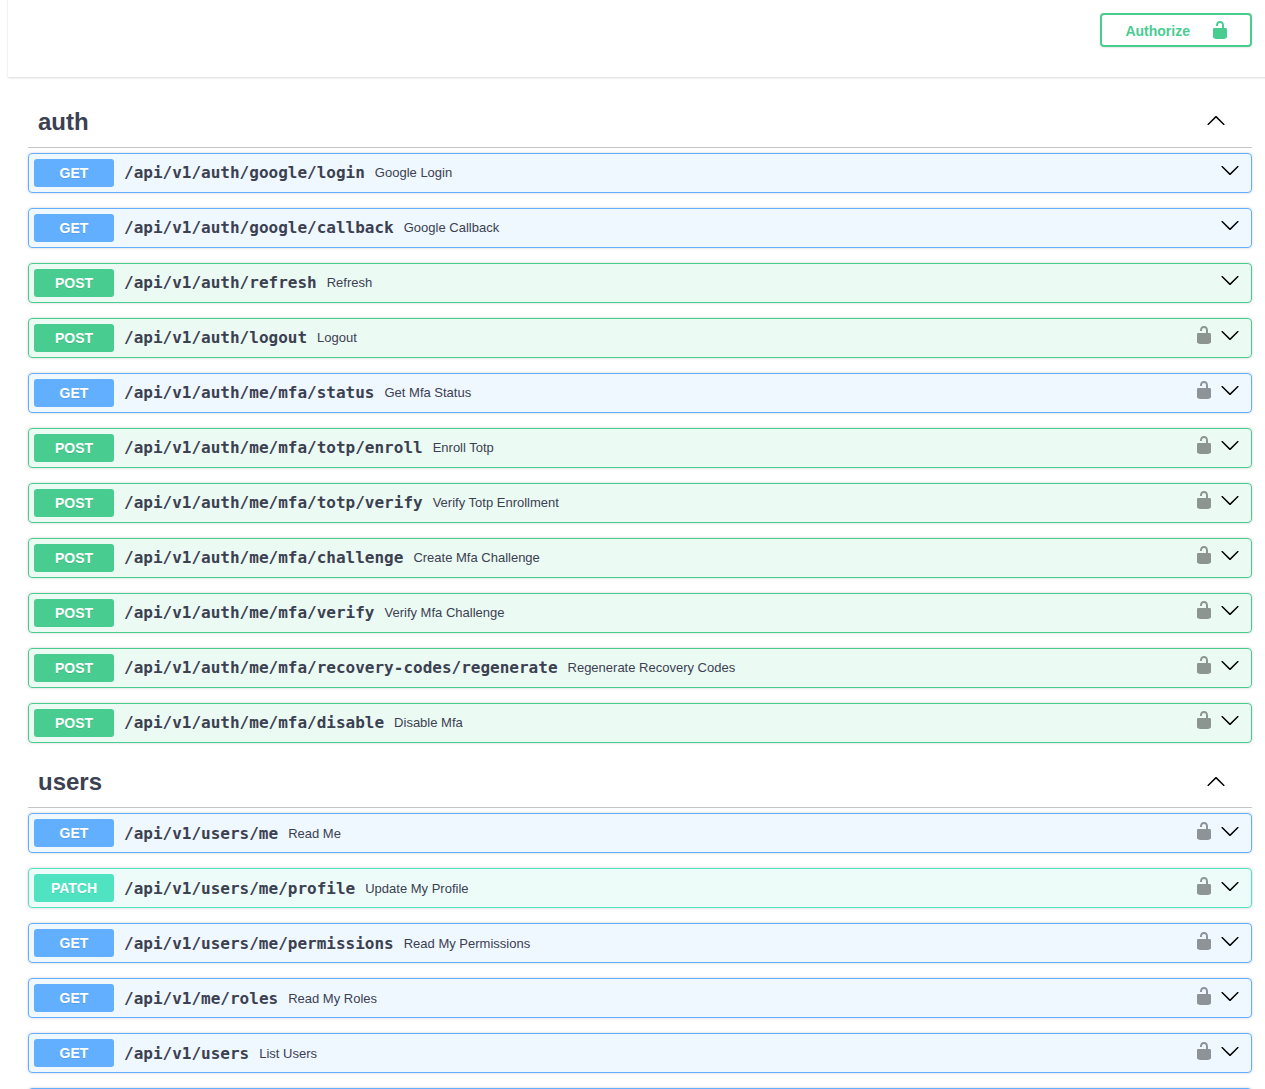
\includegraphics[width=\textwidth,height=0.82\textheight,keepaspectratio]{graphics/swagger/01_auth.png}
    \caption{Swagger UI --- Authentication endpoints. Google OAuth login/callback, refresh, logout, and TOTP-based MFA enrolment, challenge, verify, recovery-code regeneration, and disable.}
    \label{fig:swagger_01_auth}
\end{figure}

\begin{figure}[H]
    \centering
    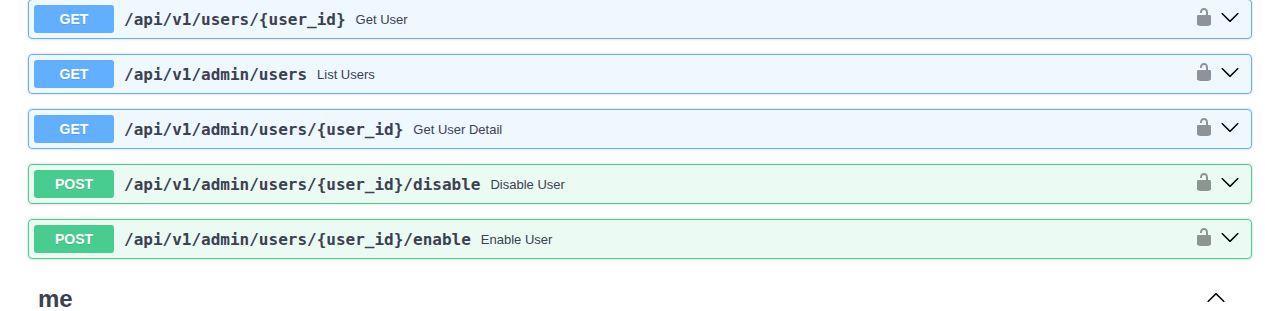
\includegraphics[width=\textwidth,height=0.82\textheight,keepaspectratio]{graphics/swagger/02_mfa.png}
    \caption{Swagger UI --- MFA management. Self-service multi-factor authentication endpoints under \texttt{/auth/me/mfa}.}
    \label{fig:swagger_02_mfa}
\end{figure}

\begin{figure}[H]
    \centering
    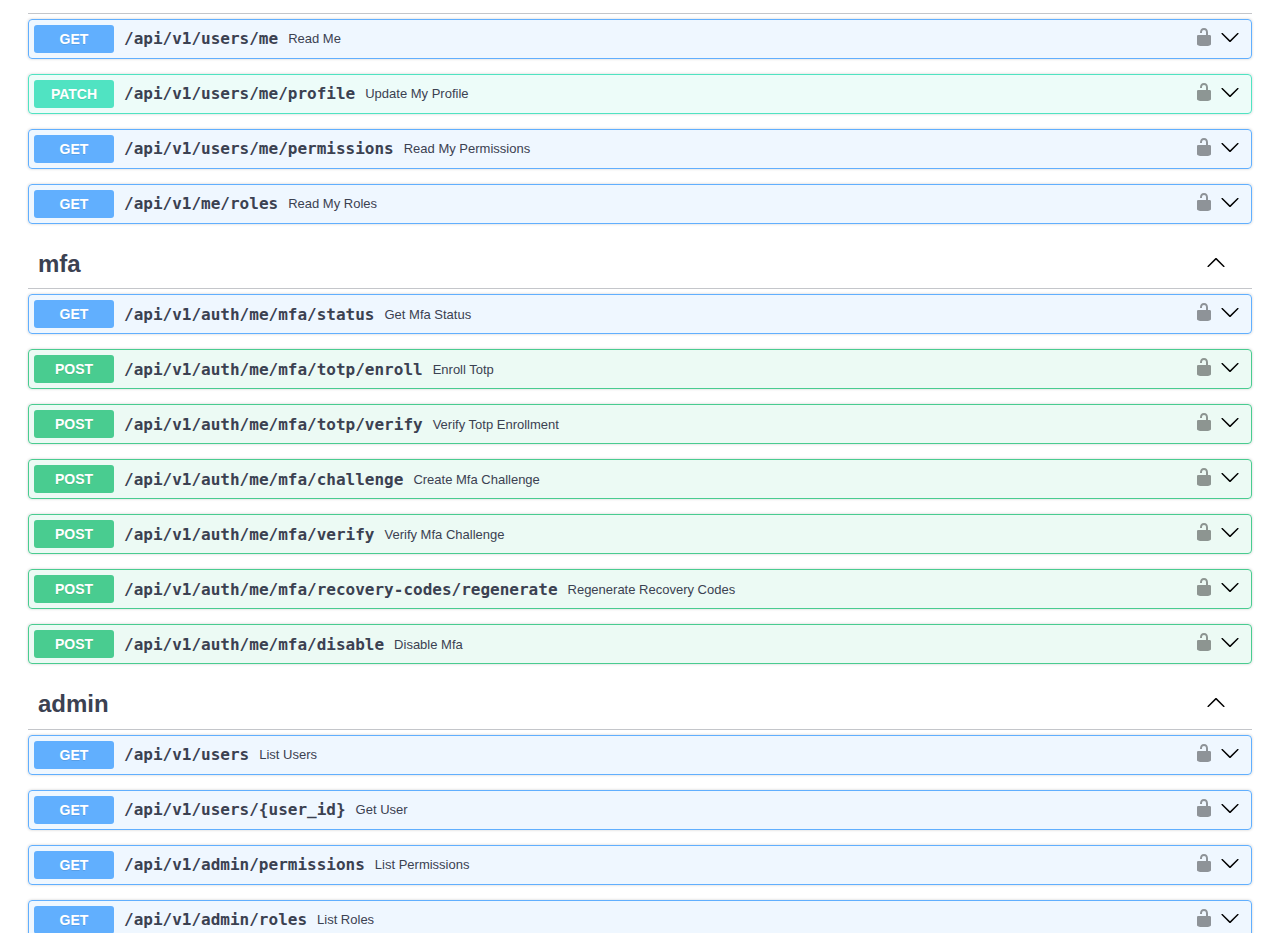
\includegraphics[width=\textwidth,height=0.82\textheight,keepaspectratio]{graphics/swagger/03a_admin_part1.png}
    \caption{Swagger UI --- Administration --- part 1. First half of the administrative endpoint surface (user disable/enable, audit subset).}
    \label{fig:swagger_03a_admin_part1}
\end{figure}

\begin{figure}[H]
    \centering
    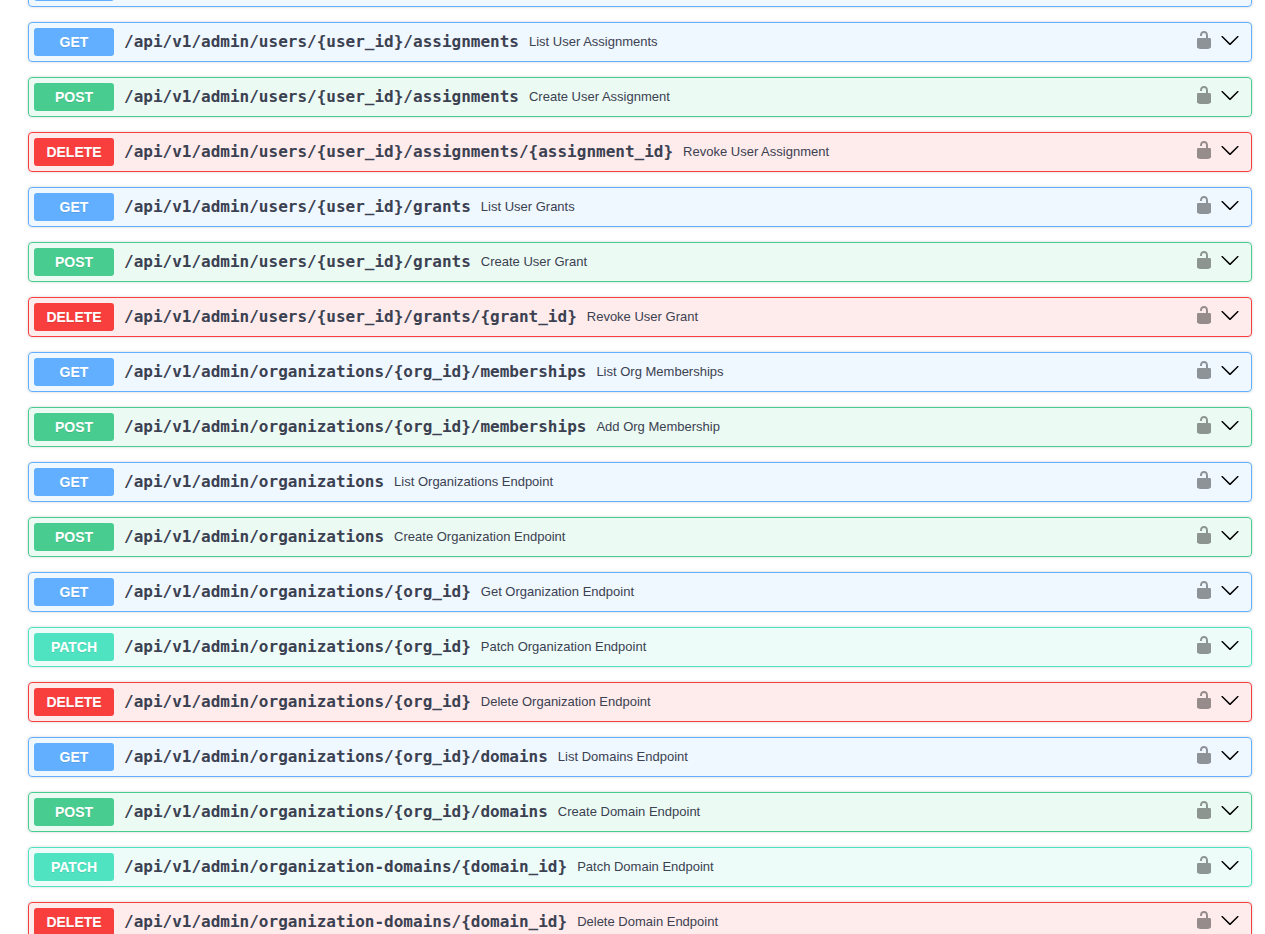
\includegraphics[width=\textwidth,height=0.82\textheight,keepaspectratio]{graphics/swagger/03b_admin_part2.png}
    \caption{Swagger UI --- Administration --- part 2. Remaining administrative endpoints (continued from previous figure).}
    \label{fig:swagger_03b_admin_part2}
\end{figure}

\begin{figure}[H]
    \centering
    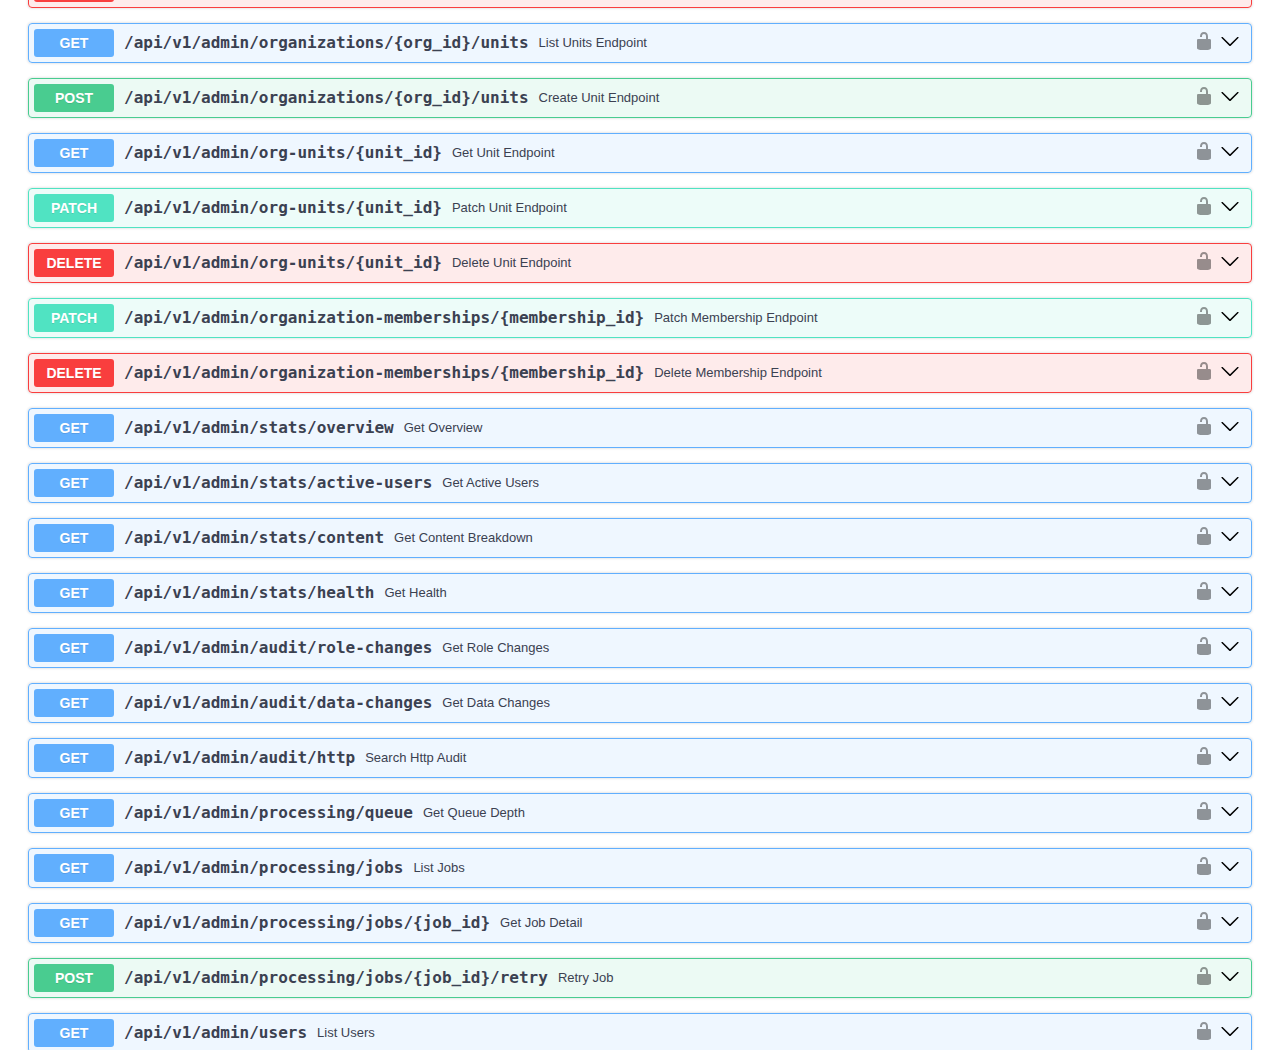
\includegraphics[width=\textwidth,height=0.82\textheight,keepaspectratio]{graphics/swagger/04_access_control.png}
    \caption{Swagger UI --- Access control \& roles. Role assignments, permission grants, organisation-scoped role queries.}
    \label{fig:swagger_04_access_control}
\end{figure}

\begin{figure}[H]
    \centering
    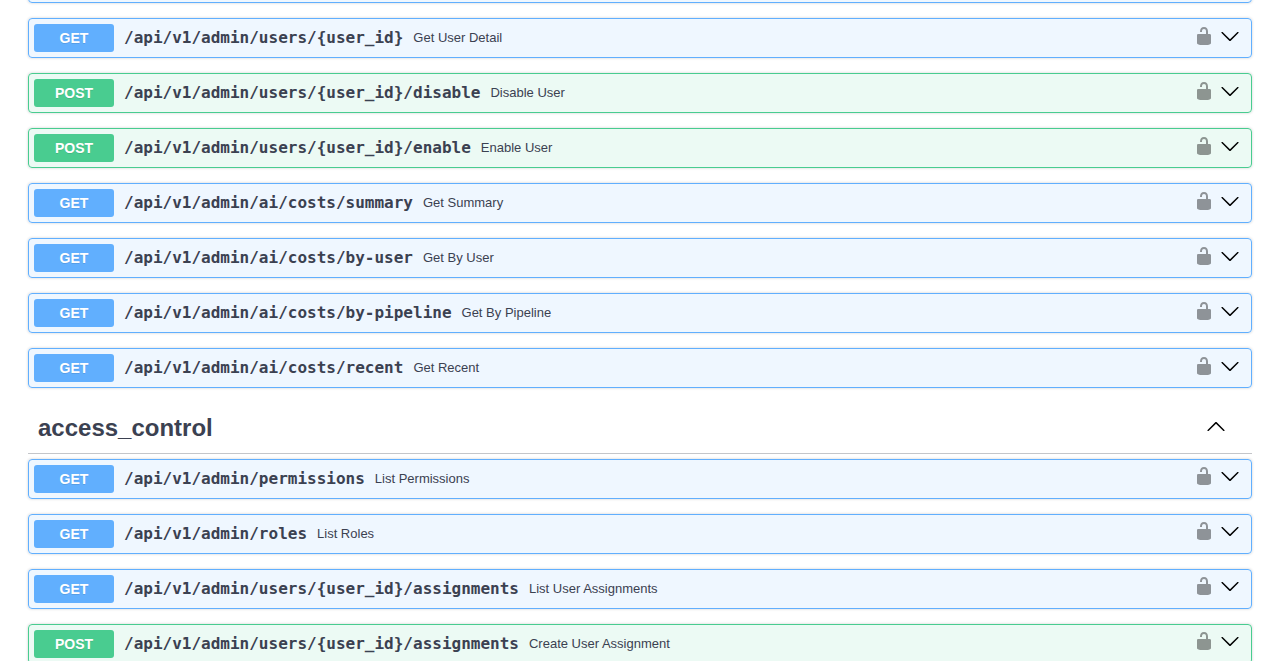
\includegraphics[width=\textwidth,height=0.82\textheight,keepaspectratio]{graphics/swagger/05_organizations.png}
    \caption{Swagger UI --- Organisations. Organisational unit CRUD, hierarchy walk, member listing.}
    \label{fig:swagger_05_organizations}
\end{figure}

\begin{figure}[H]
    \centering
    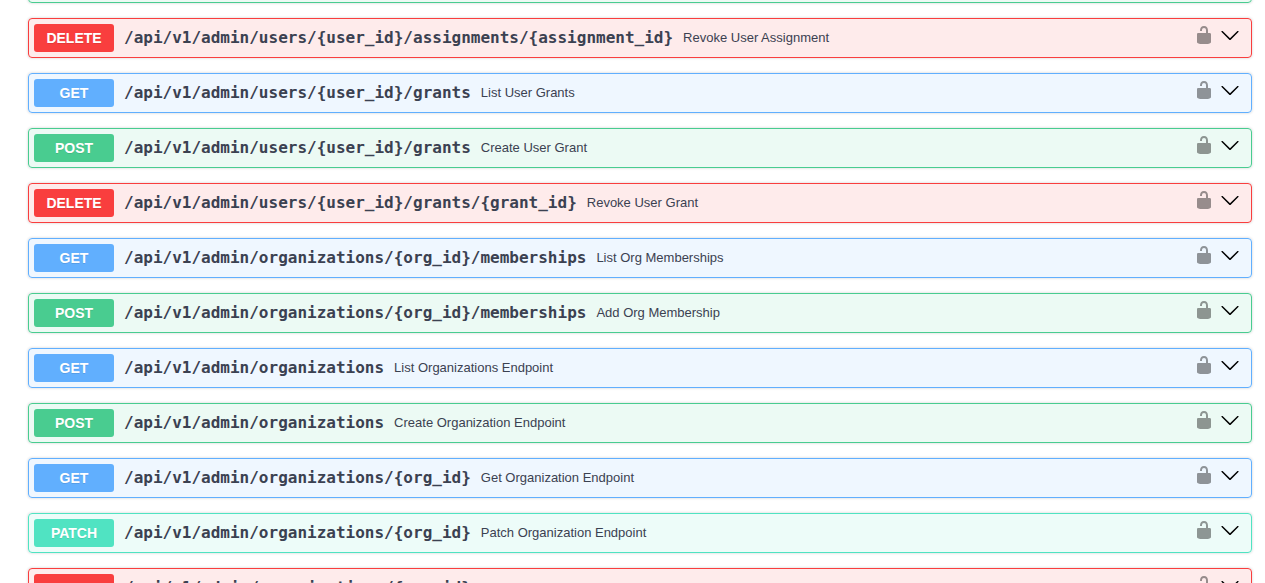
\includegraphics[width=\textwidth,height=0.82\textheight,keepaspectratio]{graphics/swagger/06_courses_learner.png}
    \caption{Swagger UI --- Courses --- learner. Published-course catalogue, enrolled-course lookup, and lesson tree for the calling student.}
    \label{fig:swagger_06_courses_learner}
\end{figure}

\begin{figure}[H]
    \centering
    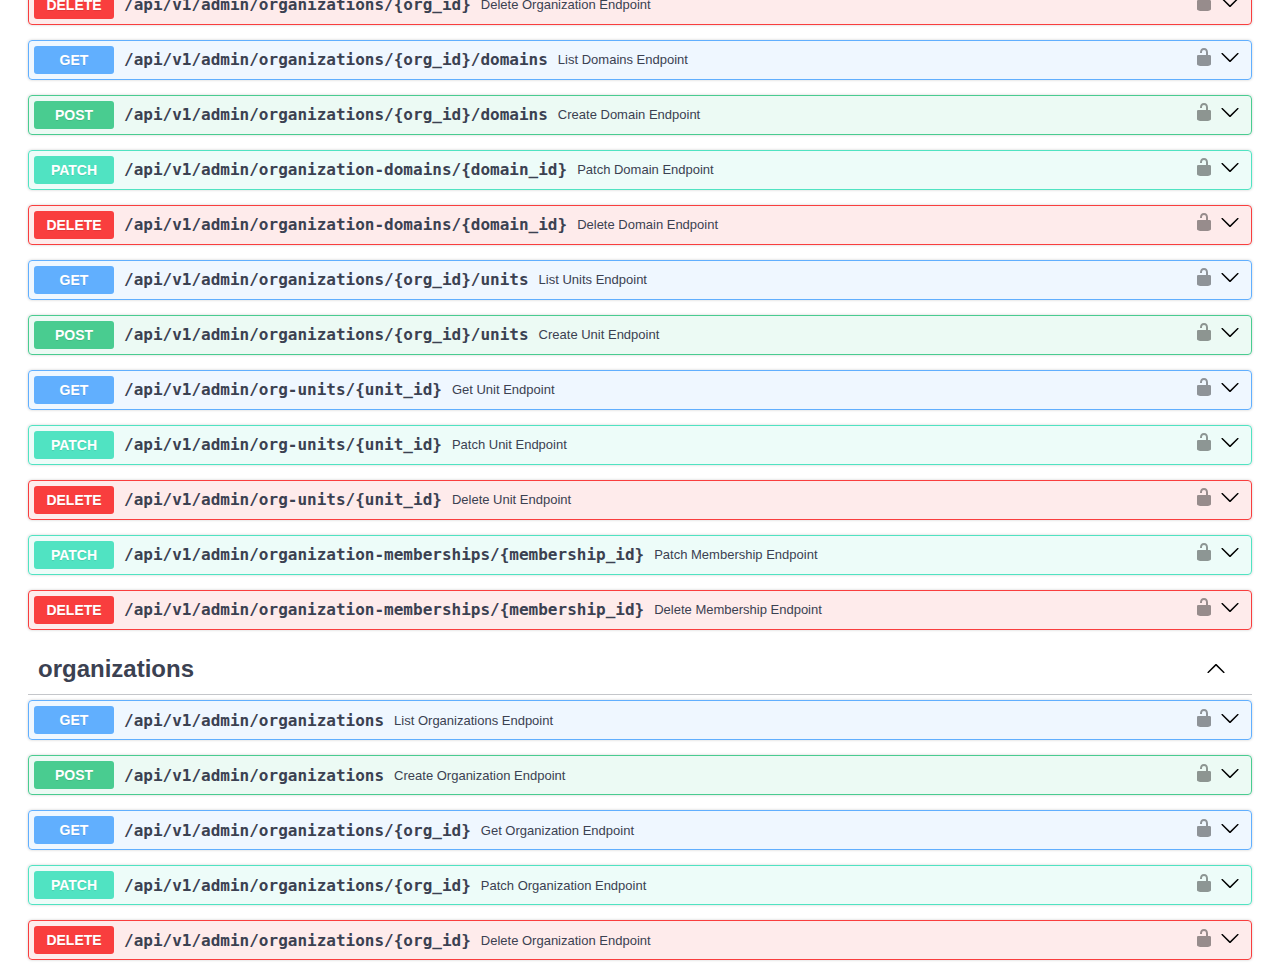
\includegraphics[width=\textwidth,height=0.82\textheight,keepaspectratio]{graphics/swagger/07_courses_authoring.png}
    \caption{Swagger UI --- Courses --- authoring. Instructor course creation, module/lesson editing, publish/archive lifecycle, roster, prerequisites, item reordering.}
    \label{fig:swagger_07_courses_authoring}
\end{figure}

\begin{figure}[H]
    \centering
    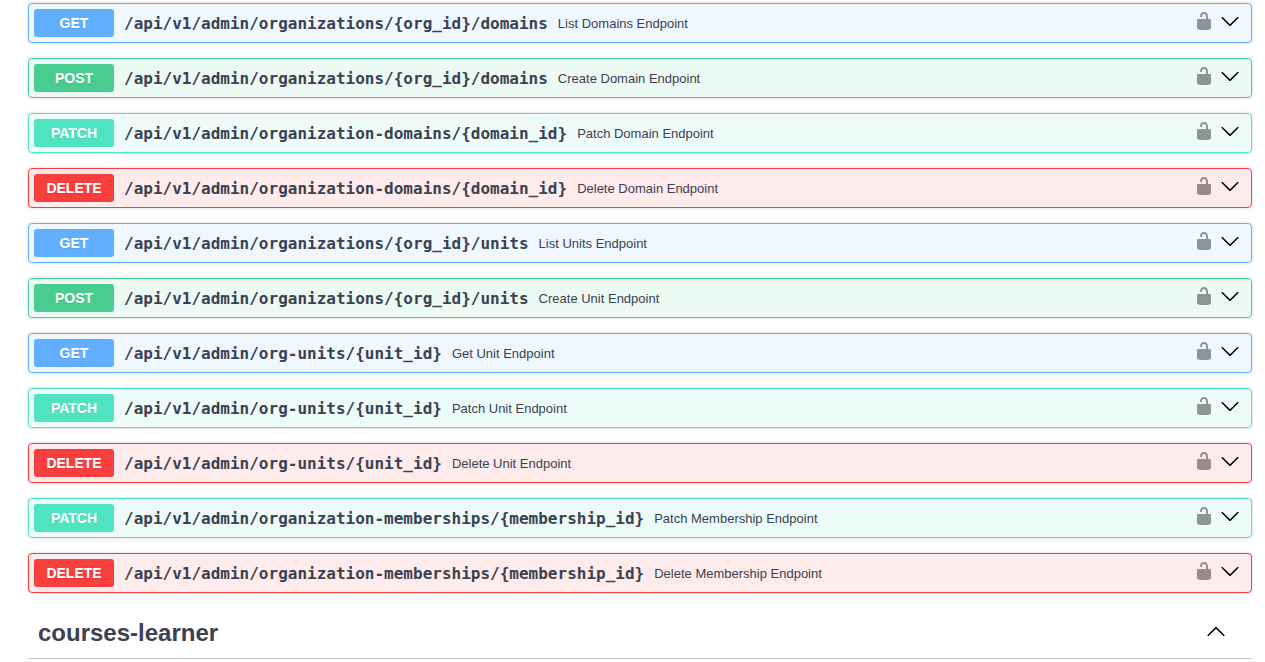
\includegraphics[width=\textwidth,height=0.82\textheight,keepaspectratio]{graphics/swagger/08_courses_admin.png}
    \caption{Swagger UI --- Courses --- department \& administration. Department-scoped course assignment to teachers, cross-organisation course listing, soft-delete restoration, and audit views.}
    \label{fig:swagger_08_courses_admin}
\end{figure}

\begin{figure}[H]
    \centering
    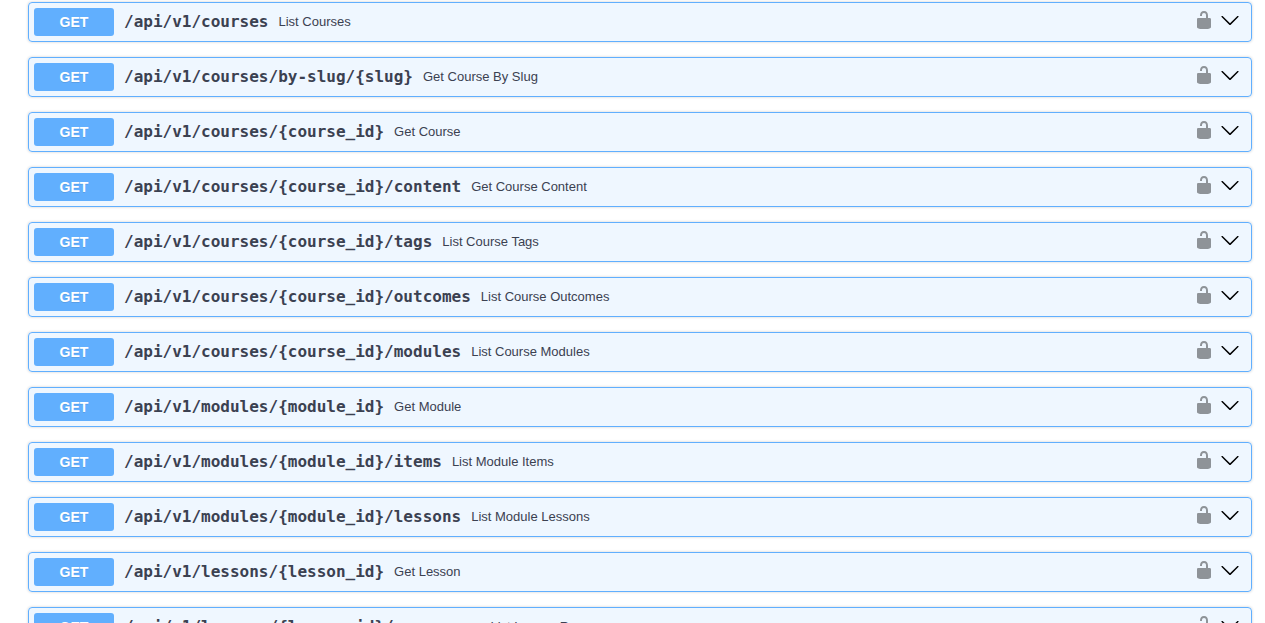
\includegraphics[width=\textwidth,height=0.82\textheight,keepaspectratio]{graphics/swagger/09_materials.png}
    \caption{Swagger UI --- Materials. Two-phase upload protocol (presigned init / multipart parts / complete), processing summaries, learner-facing presigned streaming URLs.}
    \label{fig:swagger_09_materials}
\end{figure}

\begin{figure}[H]
    \centering
    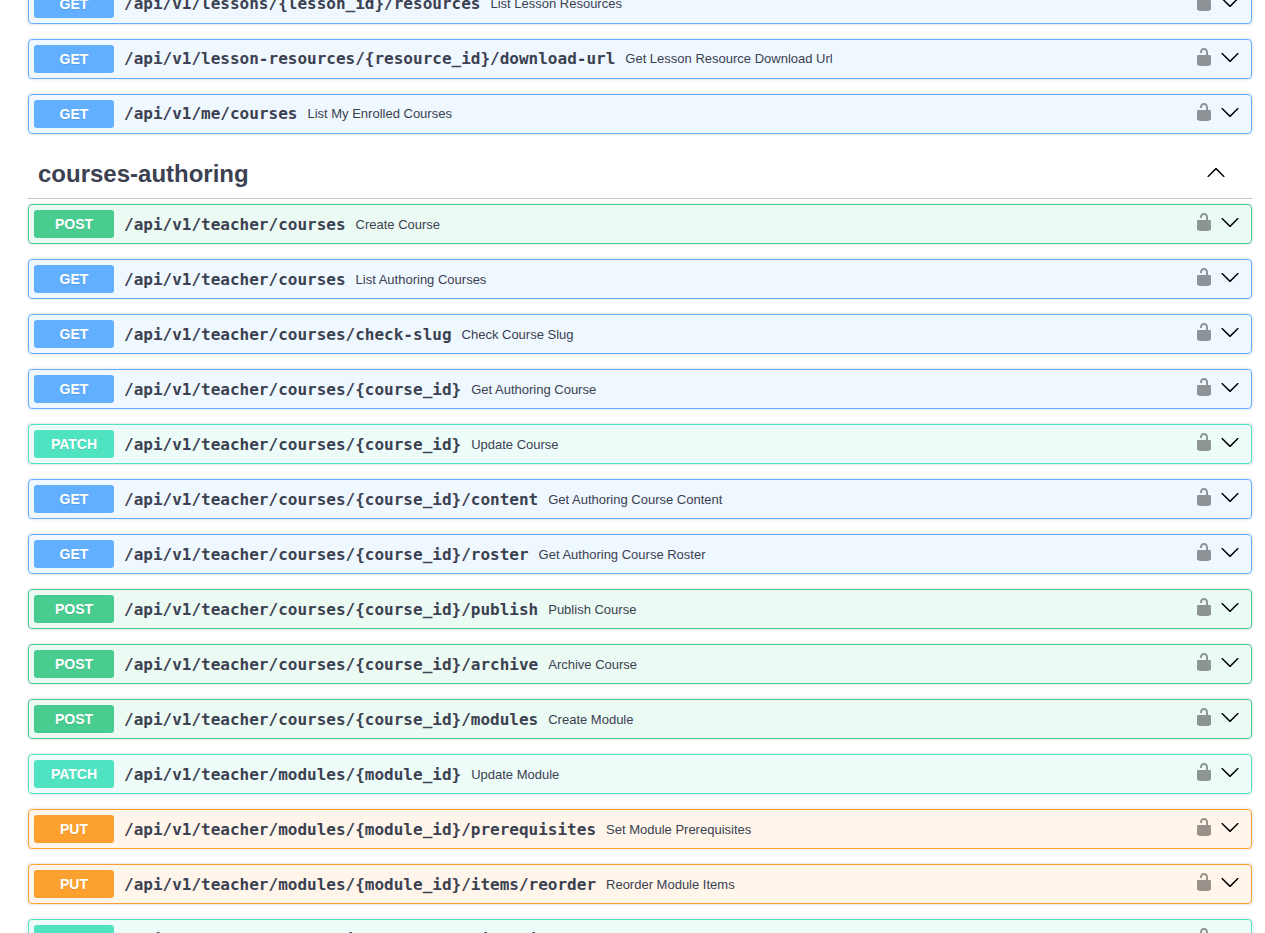
\includegraphics[width=\textwidth,height=0.82\textheight,keepaspectratio]{graphics/swagger/10_quizzes.png}
    \caption{Swagger UI --- Quizzes. Authoring (draft/generate/review/publish) and learner (start attempt, submit, results) endpoints; AI generation through \texttt{generation-runs/\{run\_id\}} polling.}
    \label{fig:swagger_10_quizzes}
\end{figure}

\begin{figure}[H]
    \centering
    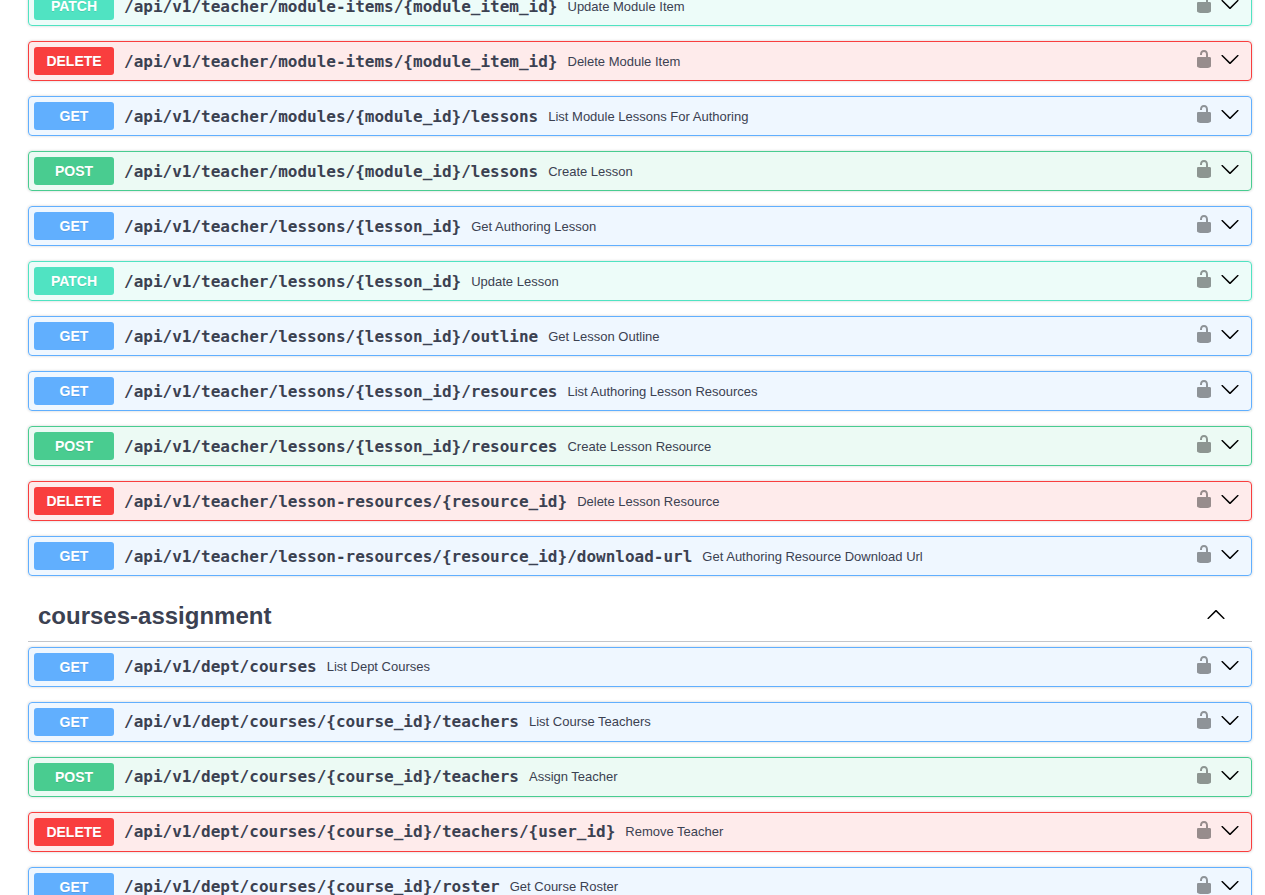
\includegraphics[width=\textwidth,height=0.82\textheight,keepaspectratio]{graphics/swagger/11_interviews.png}
    \caption{Swagger UI --- Interviews. Mock-interview authoring (slots, question banks, regeneration) and learner endpoints (start/submit/feedback).}
    \label{fig:swagger_11_interviews}
\end{figure}

\begin{figure}[H]
    \centering
    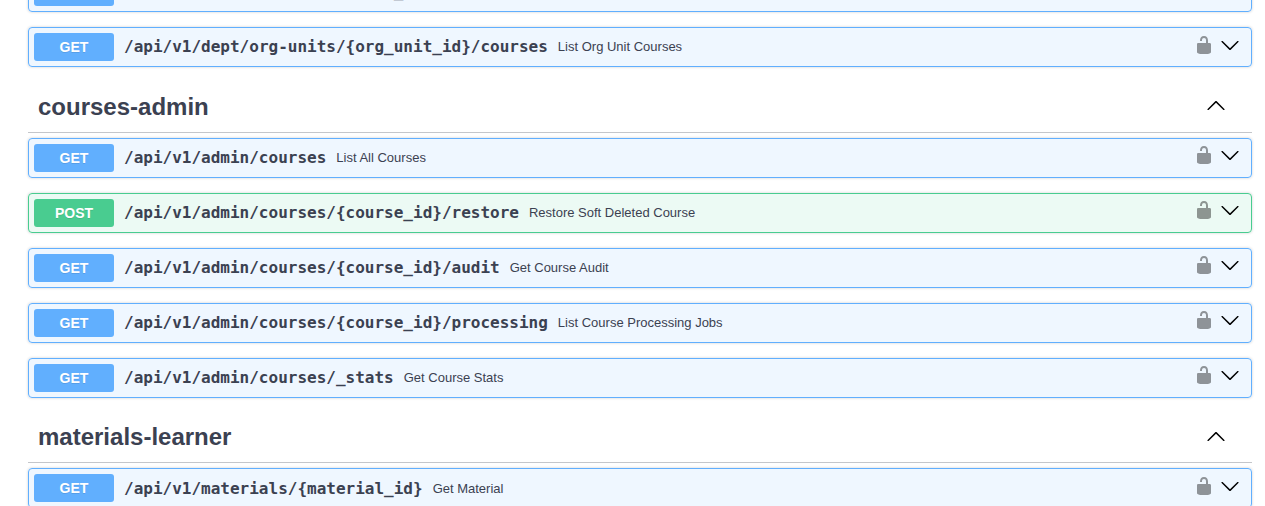
\includegraphics[width=\textwidth,height=0.82\textheight,keepaspectratio]{graphics/swagger/12_enrollments.png}
    \caption{Swagger UI --- Enrollments. Learner self-enrolment and department-assigned enrolment management.}
    \label{fig:swagger_12_enrollments}
\end{figure}

\begin{figure}[H]
    \centering
    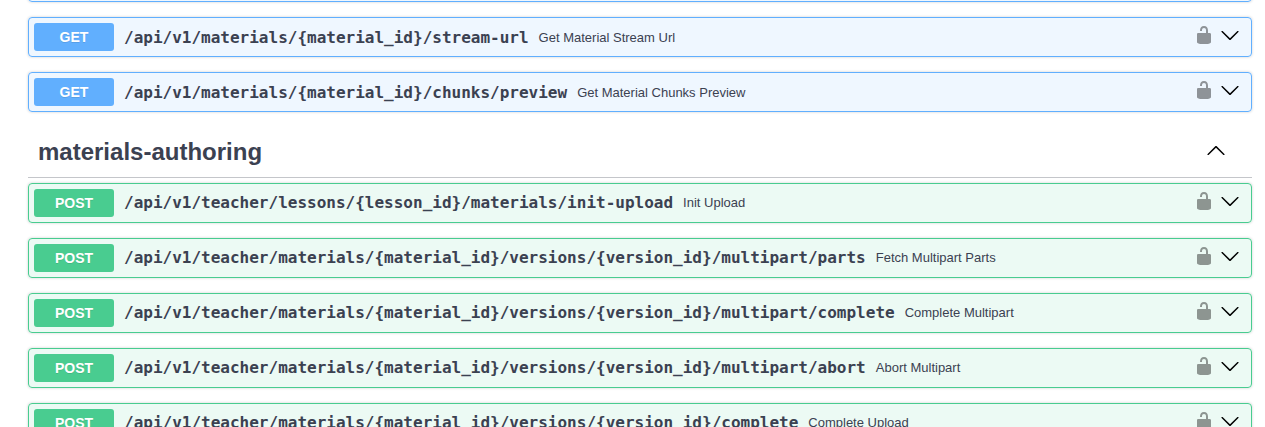
\includegraphics[width=\textwidth,height=0.82\textheight,keepaspectratio]{graphics/swagger/13_progress.png}
    \caption{Swagger UI --- Progress. Learner progress tracking and instructor progress dashboards.}
    \label{fig:swagger_13_progress}
\end{figure}

\begin{figure}[H]
    \centering
    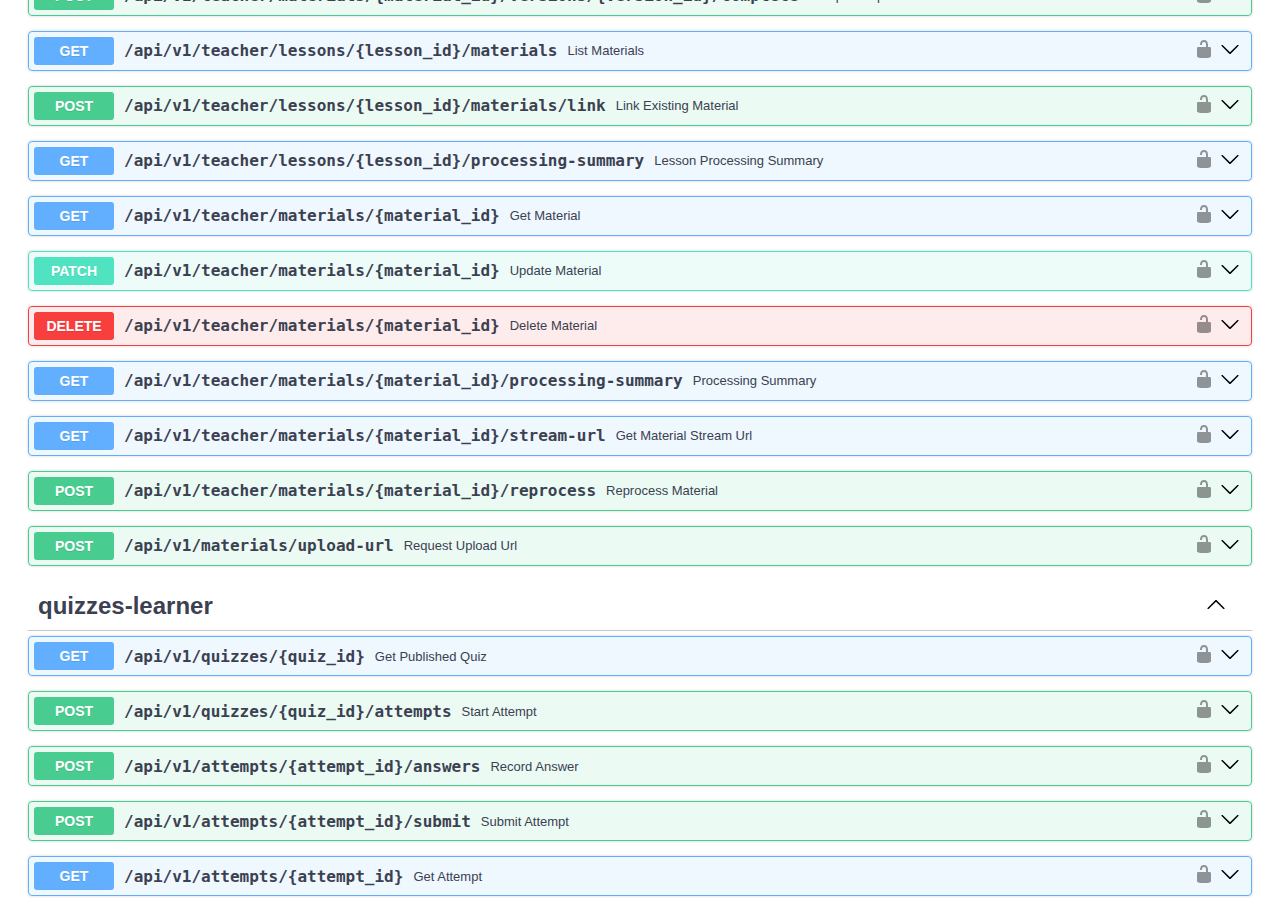
\includegraphics[width=\textwidth,height=0.82\textheight,keepaspectratio]{graphics/swagger/14_career_paths.png}
    \caption{Swagger UI --- Career paths. Published career-path catalogue (learner) and authoring routes (instructor/admin).}
    \label{fig:swagger_14_career_paths}
\end{figure}

\begin{figure}[H]
    \centering
    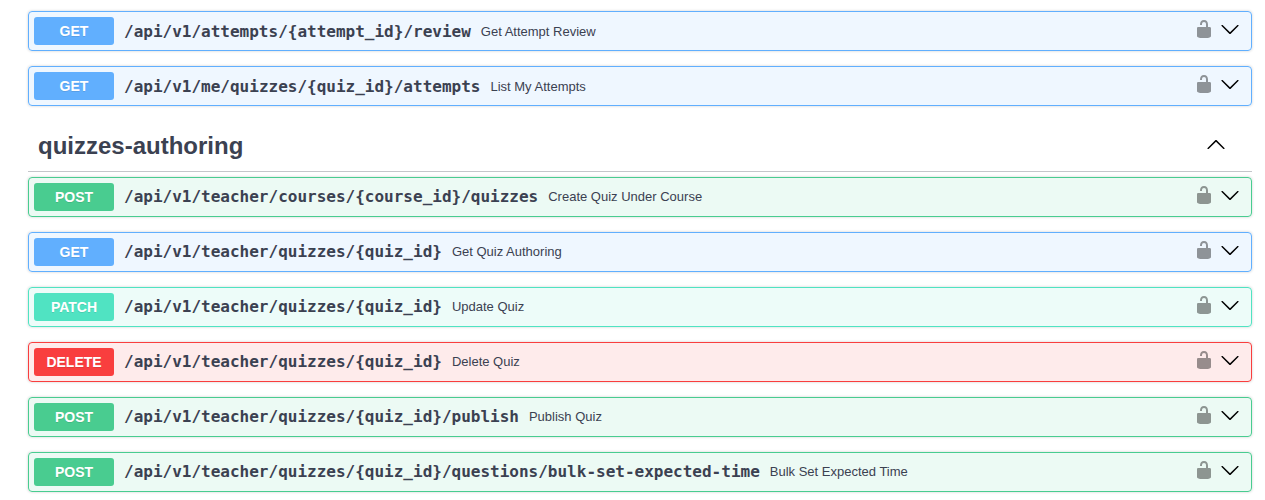
\includegraphics[width=\textwidth,height=0.82\textheight,keepaspectratio]{graphics/swagger/15_notifications.png}
    \caption{Swagger UI --- Notifications \& stats. Learner notification inbox (cursor-paginated by \texttt{created\_at}) and admin platform-wide statistics.}
    \label{fig:swagger_15_notifications}
\end{figure}

\begin{figure}[H]
    \centering
    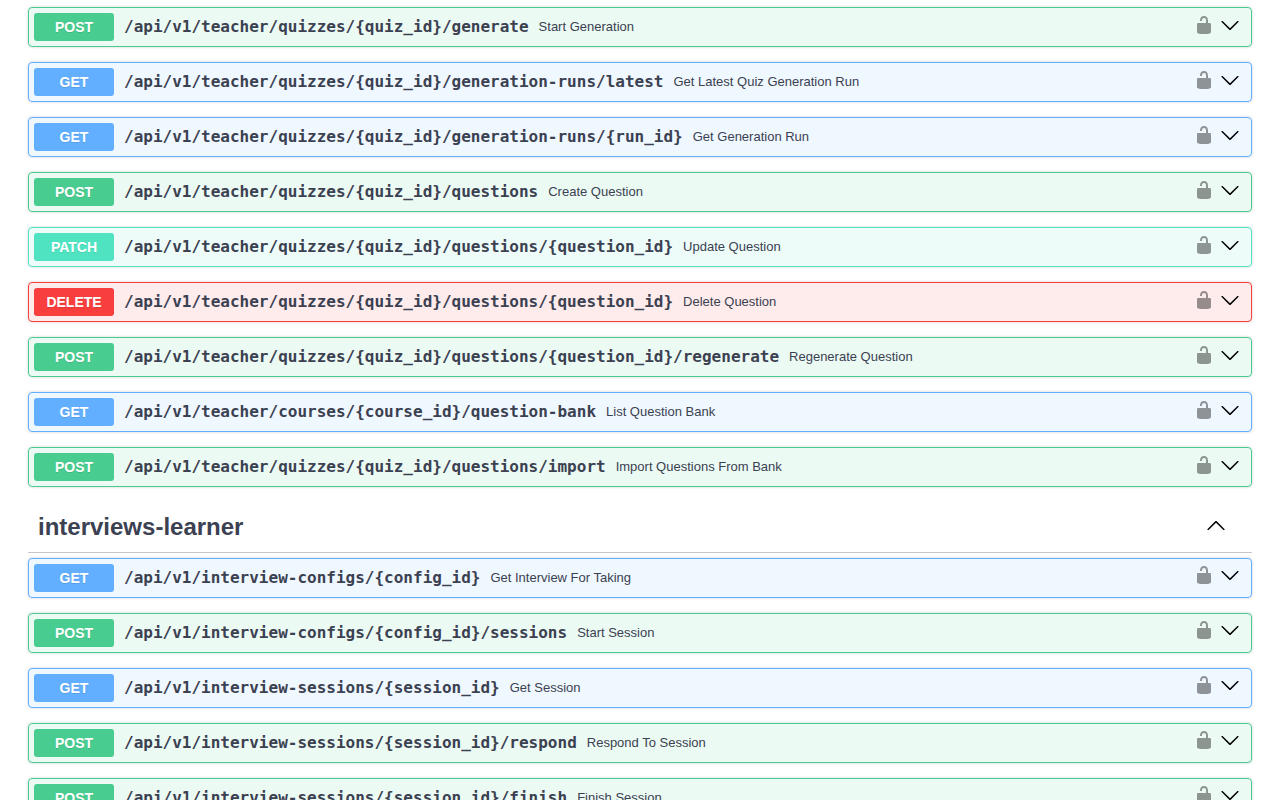
\includegraphics[width=\textwidth,height=0.82\textheight,keepaspectratio]{graphics/swagger/16_audit_processing.png}
    \caption{Swagger UI --- Audit \& processing. Cross-feature audit log queries and AI-processing run inspection (admin).}
    \label{fig:swagger_16_audit_processing}
\end{figure}

\begin{figure}[H]
    \centering
    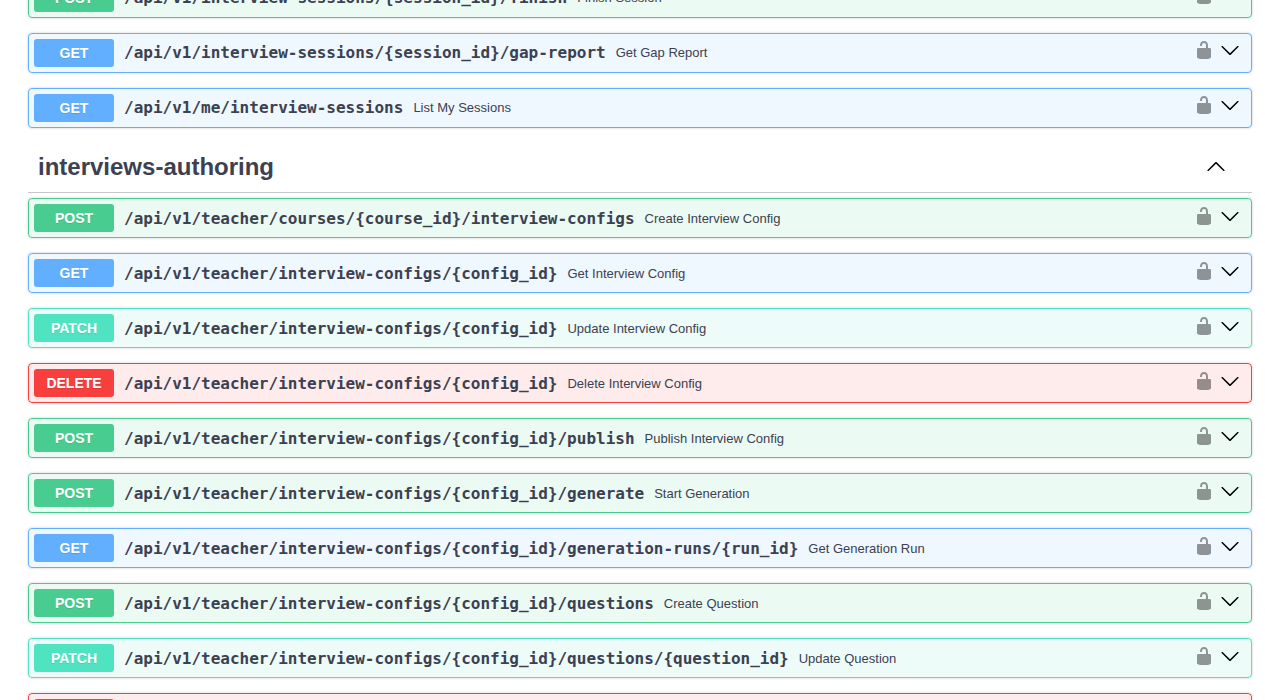
\includegraphics[width=\textwidth,height=0.82\textheight,keepaspectratio]{graphics/swagger/17_spaced_repetition.png}
    \caption{Swagger UI --- Spaced repetition. Learner card-due queue, review submission, lesson-unlock checks, and instructor analytics.}
    \label{fig:swagger_17_spaced_repetition}
\end{figure}

\begin{figure}[H]
    \centering
    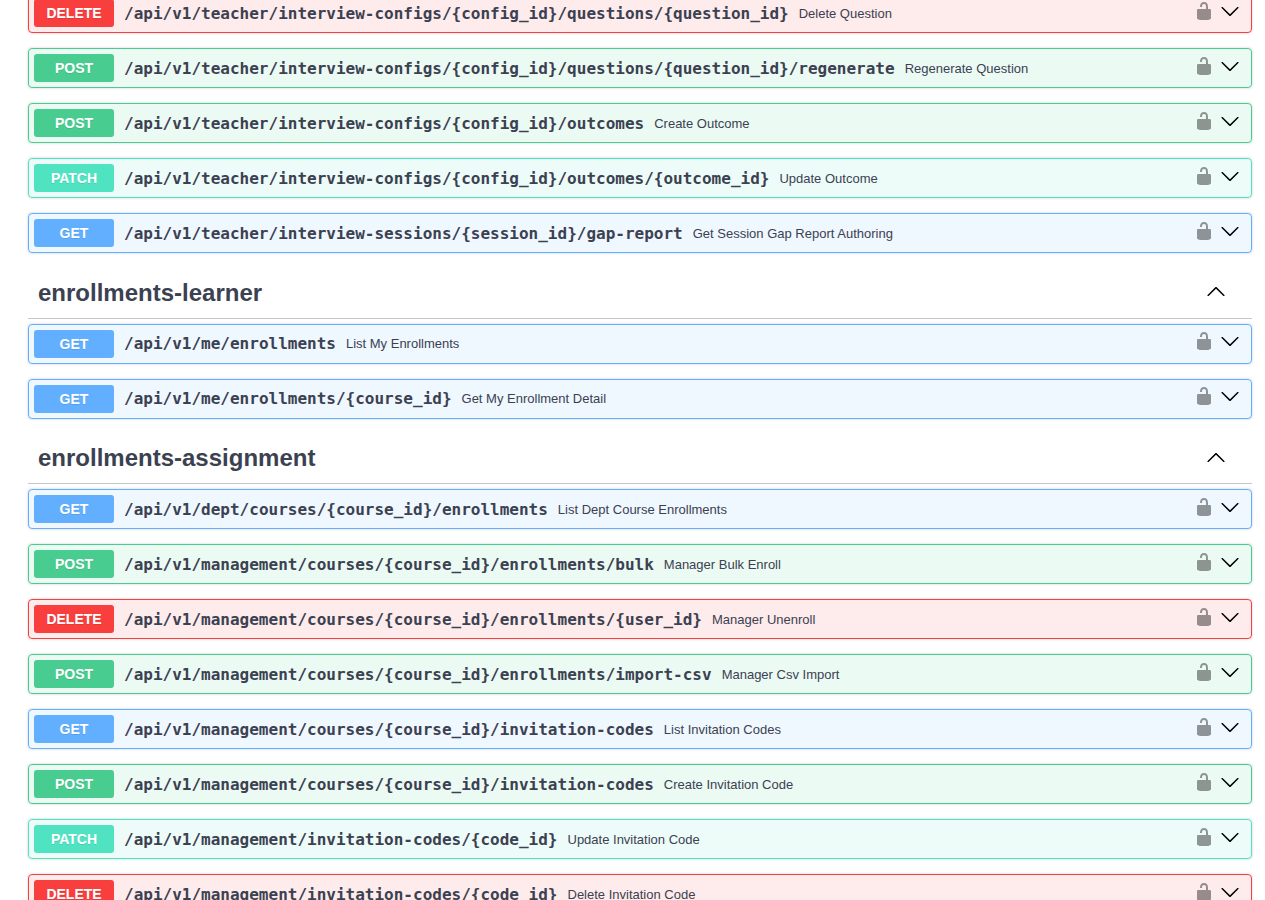
\includegraphics[width=\textwidth,height=0.82\textheight,keepaspectratio]{graphics/swagger/18_ai_costs_health.png}
    \caption{Swagger UI --- AI costs \& health. AI-cost telemetry endpoints and Kubernetes liveness/readiness probes (\texttt{/healthz}, \texttt{/readyz}).}
    \label{fig:swagger_18_ai_costs_health}
\end{figure}

\begin{figure}[H]
    \centering
    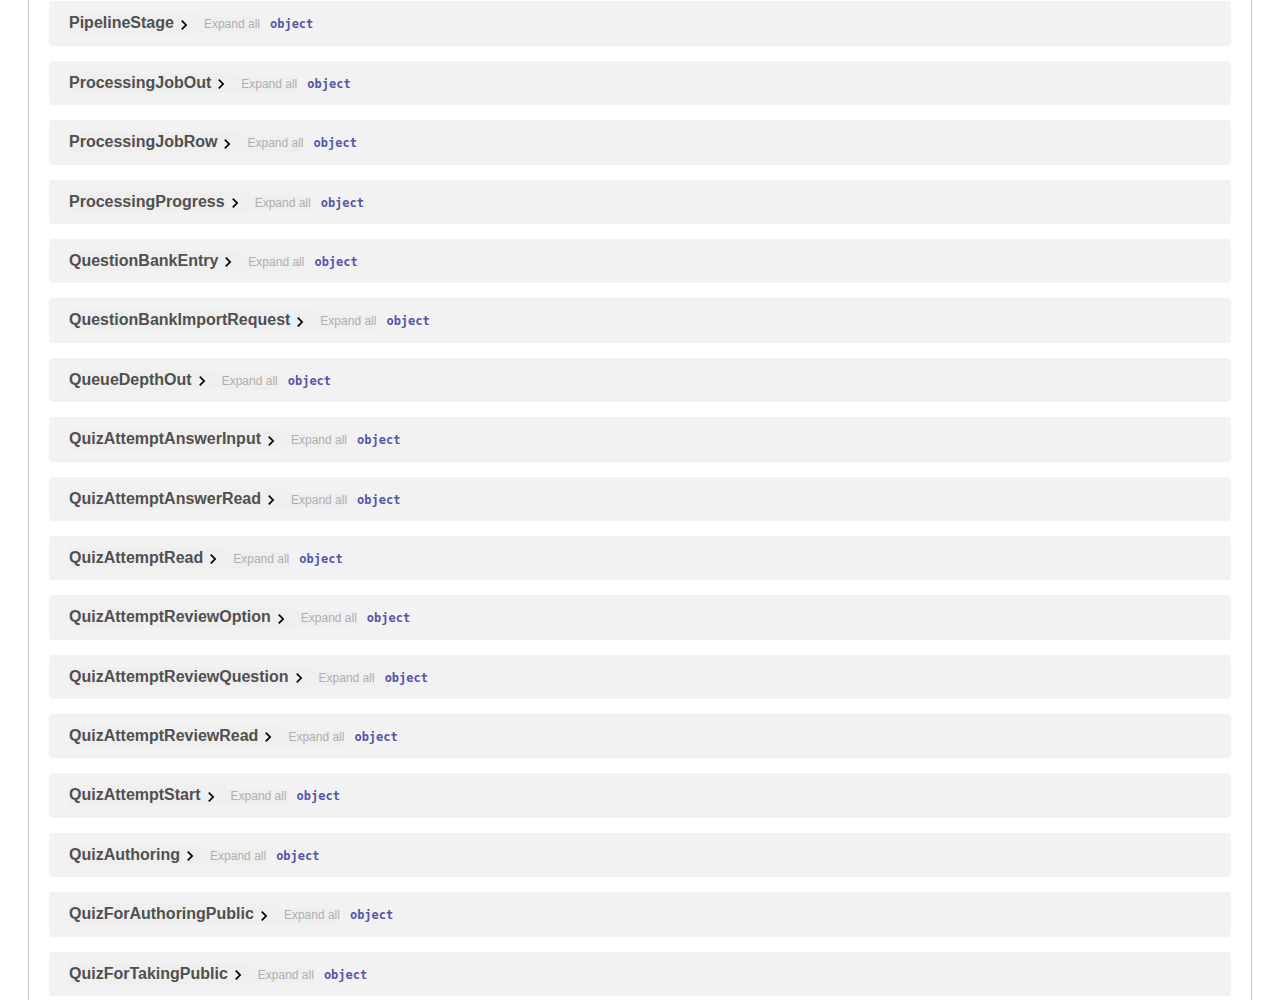
\includegraphics[width=\textwidth,height=0.82\textheight,keepaspectratio]{graphics/swagger/19a_models_part1.png}
    \caption{Swagger UI --- Schemas --- part 1. Pydantic v2 schemas exposed in OpenAPI \texttt{components.schemas} (first third of 223 schemas).}
    \label{fig:swagger_19a_models_part1}
\end{figure}

\begin{figure}[H]
    \centering
    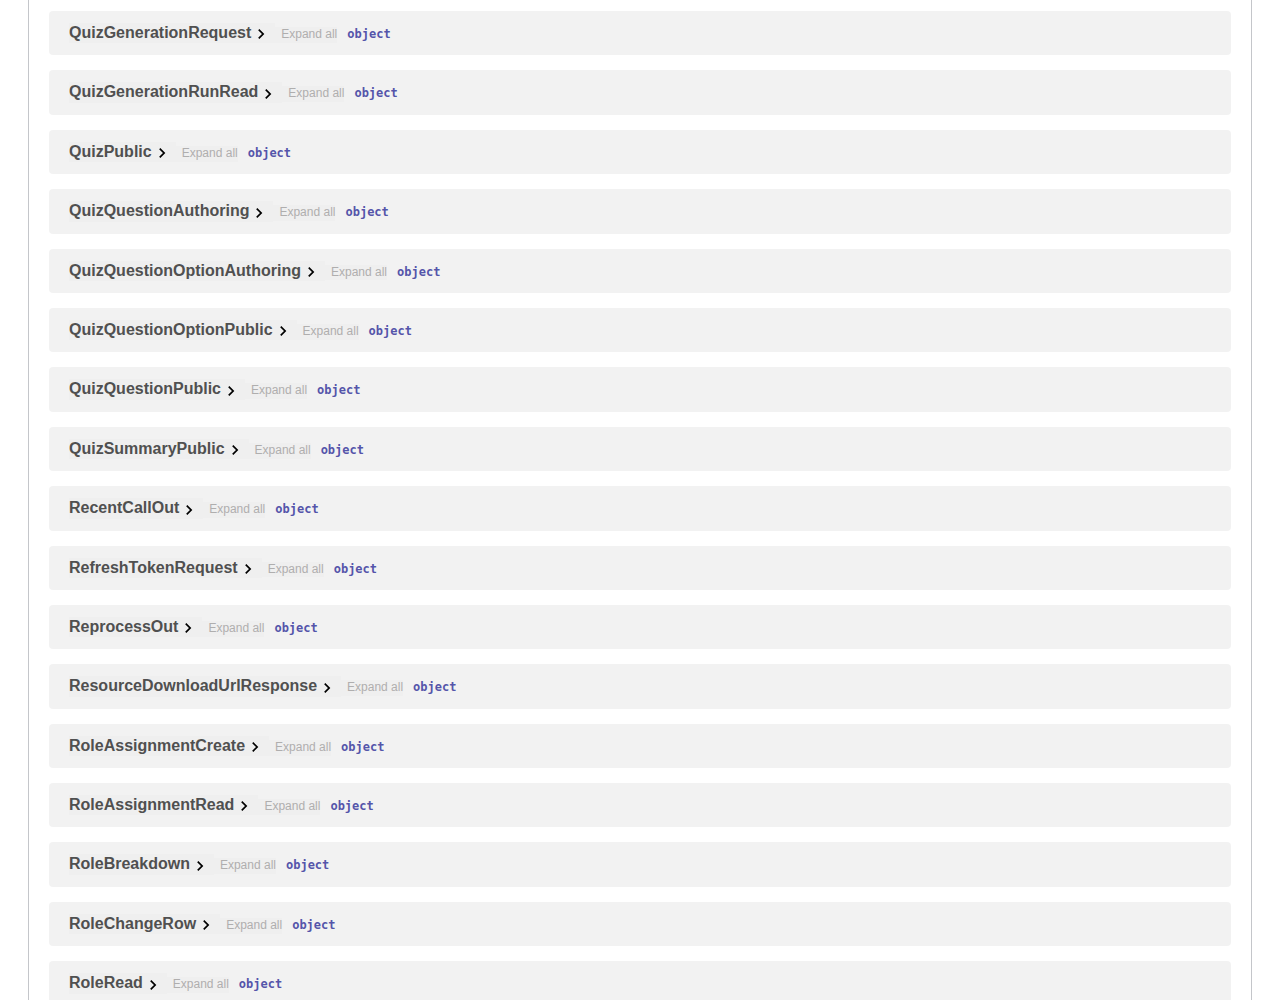
\includegraphics[width=\textwidth,height=0.82\textheight,keepaspectratio]{graphics/swagger/19b_models_part2.png}
    \caption{Swagger UI --- Schemas --- part 2. Pydantic v2 schemas (continued).}
    \label{fig:swagger_19b_models_part2}
\end{figure}

\begin{figure}[H]
    \centering
    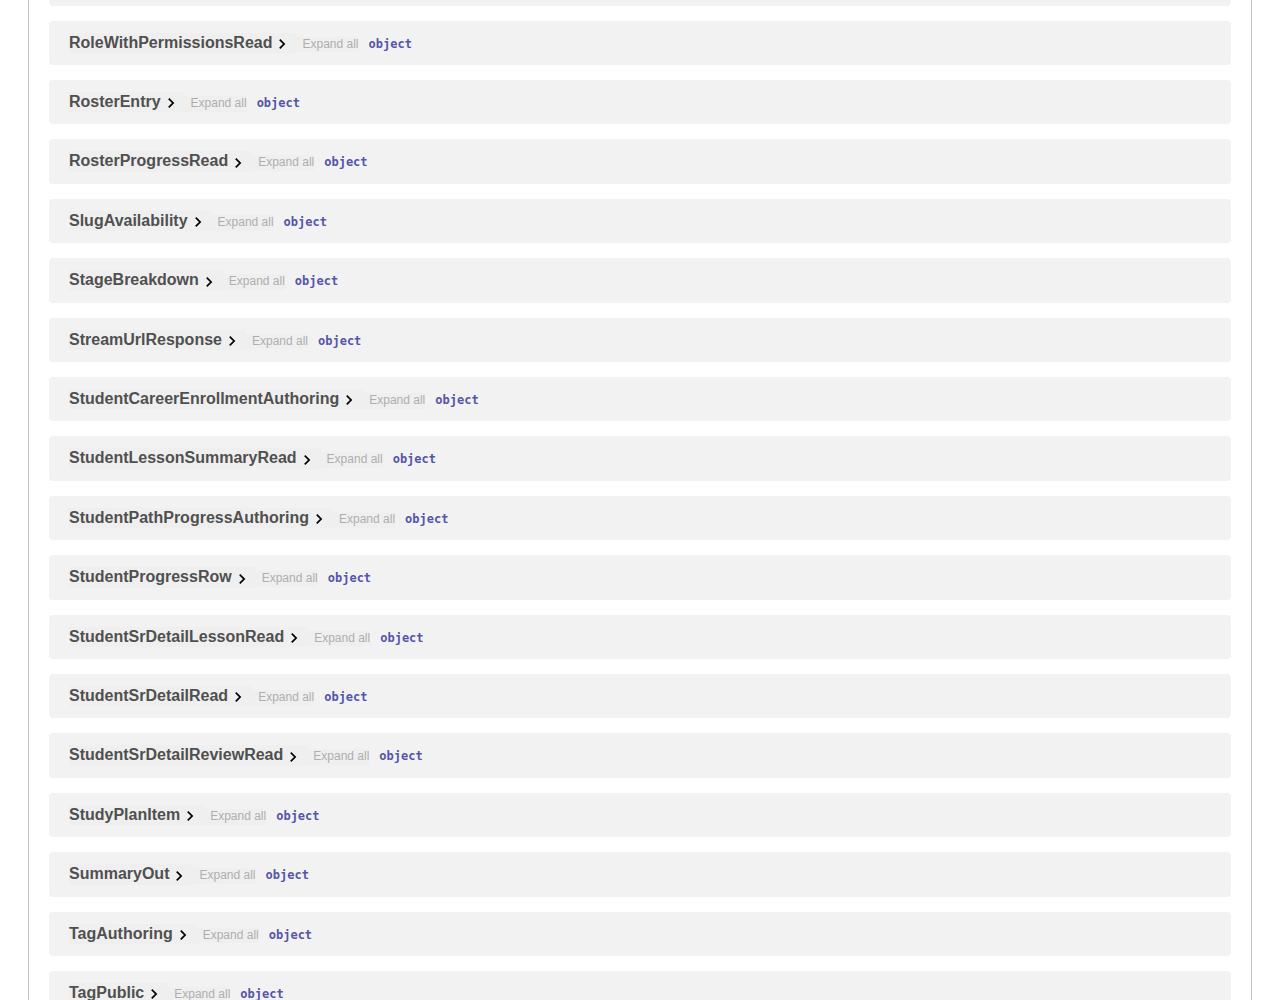
\includegraphics[width=\textwidth,height=0.82\textheight,keepaspectratio]{graphics/swagger/19c_models_part3.png}
    \caption{Swagger UI --- Schemas --- part 3. Pydantic v2 schemas (final third).}
    \label{fig:swagger_19c_models_part3}
\end{figure}

% ────────────────────────────────────────────────────────────
\subsection{Learning Programs}

A learning programme bundles career paths into a single enrolment. Authoring is version-based: edits land on an open draft and publishing freezes it, so a student who enrolled under version~2 continues to see version~2. Enrolment places a student on the programme version's default path at once; further paths may be added directly, up to the limit the version declares. The request endpoints implement the dean-review workflow by which a student leaves a path --- moving to another without losing progress on courses the two share, or dropping one outright --- and both kinds share one queue, one open-request slot and one switch allowance.

\renewcommand{\arraystretch}{1.12}
\small
\begin{longtable}{|>{\raggedright\arraybackslash}m{0.07\textwidth}|>{\raggedright\arraybackslash}m{0.45\textwidth}|>{\raggedright\arraybackslash}m{0.38\textwidth}|}
\caption{Learning Programs endpoints.}
\label{tab:api_learning_programs} \\
\hline
\textbf{Method} & \textbf{Path} & \textbf{Purpose} \\ \hline
\endfirsthead
\multicolumn{3}{c}{{\bfseries Table \thetable\ -- Continued}} \\ \hline
\textbf{Method} & \textbf{Path} & \textbf{Purpose} \\ \hline
\endhead
\hline
\endfoot

\texttt{GET} & \path|/management/learning-programs/options| & Faculties and career paths available when authoring, scoped to the manager's organisation. \\ \hline
\texttt{POST} & \path|/management/learning-programs| & Create a programme as a draft version 1. \\ \hline
\texttt{GET} & \path|/management/learning-programs| & List programmes the caller manages. \\ \hline
\texttt{GET} & \path|/management/learning-programs/{program\_id}| & Programme detail with its current version and constituent paths. \\ \hline
\texttt{GET} & \path|/management/learning-programs/{program\_id}/versions| & Version history; publishing freezes a version and opens the next draft. \\ \hline
\texttt{GET} & \path|/management/learning-programs/{program\_id}/versions/{version\_id}| & One frozen version, as enrolled students see it. \\ \hline
\texttt{PATCH} & \path|/management/learning-programs/{program\_id}| & Edit the open draft. A published version is immutable. \\ \hline
\texttt{POST} & \path|/management/learning-programs/{program\_id}/publish| & Publish the draft; existing enrolments stay on the version they joined. \\ \hline
\texttt{POST} & \path|/management/learning-programs/{program\_id}/archive| & Archive the programme; no new enrolments, existing ones continue. \\ \hline
\texttt{GET} & \path|/management/learning-programs/{program\_id}/students| & Enrolment roster with each student's held paths and progress. \\ \hline
\texttt{POST} & \path|/management/learning-programs/{program\_id}/students| & Enrol students individually; rejected as a whole if the concurrency cap would be exceeded. \\ \hline
\texttt{POST} & \path|/management/learning-programs/{program\_id}/students/import-csv| & Bulk enrol from CSV; rows are validated and reported per row. \\ \hline
\texttt{DELETE} & \path|/management/learning-programs/{program\_id}/students/{student\_id}| & Withdraw a student, releasing the course entitlements the programme granted. \\ \hline
\texttt{GET} & \path|/management/learning-programs/{program\_id}/path-change-requests| & Pending and decided path requests, of both kinds, for dean review. \\ \hline
\texttt{POST} & \path|/management/learning-programs/path-change-requests/{request\_id}/in-progress| & Acknowledge a request so the student sees it is being considered. \\ \hline
\texttt{POST} & \path|/management/learning-programs/path-change-requests/{request\_id}/approve| & Approve. A change transfers progress and re-grants entitlements for shared courses; a drop closes the path against a snapshot and grants nothing, and is refused if it would leave the student with no path in progress. \\ \hline
\texttt{POST} & \path|/management/learning-programs/path-change-requests/{request\_id}/reject| & Reject with a reason, which the student sees. \\ \hline
\texttt{GET} & \path|/me/learning-program-enrollments| & The student's own programme enrolments. \\ \hline
\texttt{POST} & \path|/me/learning-program-enrollments/{enrollment\_id}/select-path| & Take on a further career path within an enrolled programme, up to the version's limit. Needs no approval. \\ \hline
\texttt{POST} & \path|/me/learning-program-enrollments/{enrollment\_id}/path-change-requests| & Request a change of path; queued for dean review. \\ \hline
\texttt{POST} & \path|/me/learning-program-enrollments/{enrollment\_id}/path-drop-requests| & Request that one held path be dropped with no replacement; refused while it is the student's only path in progress. \\ \hline
\texttt{DELETE} & \path|/me/learning-program-enrollments/path-change-requests/{request\_id}| & Cancel one's own pending request, of either kind, before it is decided. \\ \hline

\end{longtable}
\normalsize


% ────────────────────────────────────────────────────────────
\subsection{Policies}

Platform policies (terms, privacy, academic regulations) are authored under \path|/admin| and read under \path|/policies|. Versioning is copy-on-write --- a published version is immutable, and correcting it means opening a new draft --- so the text a reader agreed to can always be retrieved. Audience is a set of roles; an empty set means public, including signed-out visitors.

\renewcommand{\arraystretch}{1.12}
\small
\begin{longtable}{|>{\raggedright\arraybackslash}m{0.07\textwidth}|>{\raggedright\arraybackslash}m{0.45\textwidth}|>{\raggedright\arraybackslash}m{0.38\textwidth}|}
\caption{Policies endpoints.}
\label{tab:api_policies} \\
\hline
\textbf{Method} & \textbf{Path} & \textbf{Purpose} \\ \hline
\endfirsthead
\multicolumn{3}{c}{{\bfseries Table \thetable\ -- Continued}} \\ \hline
\textbf{Method} & \textbf{Path} & \textbf{Purpose} \\ \hline
\endhead
\hline
\endfoot

\texttt{GET} & \path|/policies| & Policies the reader is a party to, plus every public one. \\ \hline
\texttt{GET} & \path|/policies/{slug}| & One published policy by slug, subject to the audience filter. \\ \hline
\texttt{GET} & \path|/admin/policies| & All policies, published or not, for authoring. \\ \hline
\texttt{POST} & \path|/admin/policies| & Create a policy; version 1 opens as a draft. \\ \hline
\texttt{GET} & \path|/admin/policies/{policy\_id}| & Policy detail with its version history and audience. \\ \hline
\texttt{POST} & \path|/admin/policies/{policy\_id}/versions| & Open the next draft, seeded copy-on-write from the published text. \\ \hline
\texttt{GET} & \path|/admin/policies/{policy\_id}/versions/{version\_id}| & One version with its body, for the editor. \\ \hline
\texttt{PATCH} & \path|/admin/policies/{policy\_id}/versions/{version\_id}| & Edit the open draft; a published version is frozen. \\ \hline
\texttt{POST} & \path|/admin/policies/{policy\_id}/versions/{version\_id}/publish| & Publish a draft and retire the version it supersedes. \\ \hline
\texttt{PUT} & \path|/admin/policies/{policy\_id}/audience| & Replace the audience. An empty list makes the policy public. \\ \hline

\end{longtable}
\normalsize


% ────────────────────────────────────────────────────────────
\subsection{Discussions}

Discussion topics are opened by course managers and answered by enrolled students. A topic is scoped either to one lesson or to the course as a whole; both use the same comment, moderation and notification paths, which is why the two create endpoints differ only in their parent resource. Replies carry a parent comment, which is also what determines who is notified.

\renewcommand{\arraystretch}{1.12}
\small
\begin{longtable}{|>{\raggedright\arraybackslash}m{0.07\textwidth}|>{\raggedright\arraybackslash}m{0.45\textwidth}|>{\raggedright\arraybackslash}m{0.38\textwidth}|}
\caption{Discussions endpoints.}
\label{tab:api_discussions} \\
\hline
\textbf{Method} & \textbf{Path} & \textbf{Purpose} \\ \hline
\endfirsthead
\multicolumn{3}{c}{{\bfseries Table \thetable\ -- Continued}} \\ \hline
\textbf{Method} & \textbf{Path} & \textbf{Purpose} \\ \hline
\endhead
\hline
\endfoot

\texttt{GET} & \path|/lessons/{lesson\_id}/discussion/topics| & Topics on a lesson, for enrolled students and course managers. \\ \hline
\texttt{POST} & \path|/lessons/{lesson\_id}/discussion/topics| & Open a topic on a lesson (course managers only). \\ \hline
\texttt{GET} & \path|/courses/{course\_id}/discussion/topics| & Course-wide topics, for enrolled students and course managers. \\ \hline
\texttt{POST} & \path|/courses/{course\_id}/discussion/topics| & Open a course-wide topic (course managers only). \\ \hline
\texttt{PATCH} & \path|/discussion/topics/{topic\_id}| & Edit a topic or toggle it open/closed (course managers only). \\ \hline
\texttt{DELETE} & \path|/discussion/topics/{topic\_id}| & Soft-delete a topic and its comments (course managers only). \\ \hline
\texttt{GET} & \path|/discussion/topics/{topic\_id}/comments| & Comments on a topic, oldest first. \\ \hline
\texttt{POST} & \path|/discussion/topics/{topic\_id}/comments| & Post a comment, or a reply when a parent comment is named. \\ \hline
\texttt{PATCH} & \path|/discussion/comments/{comment\_id}| & Edit one's own comment body. \\ \hline
\texttt{DELETE} & \path|/discussion/comments/{comment\_id}| & Soft-delete a comment (author, or a manager moderating). \\ \hline

\end{longtable}
\normalsize


% ────────────────────────────────────────────────────────────
\subsection{Course Invitation Codes}

An invitation code lets a student self-enrol onto a course without a manager adding them individually. Codes carry an optional expiry and usage limit; revoking a code stops further redemptions but does not withdraw anyone already enrolled through it.

\renewcommand{\arraystretch}{1.12}
\small
\begin{longtable}{|>{\raggedright\arraybackslash}m{0.07\textwidth}|>{\raggedright\arraybackslash}m{0.45\textwidth}|>{\raggedright\arraybackslash}m{0.38\textwidth}|}
\caption{Course Invitation Codes endpoints.}
\label{tab:api_invitation_codes} \\
\hline
\textbf{Method} & \textbf{Path} & \textbf{Purpose} \\ \hline
\endfirsthead
\multicolumn{3}{c}{{\bfseries Table \thetable\ -- Continued}} \\ \hline
\textbf{Method} & \textbf{Path} & \textbf{Purpose} \\ \hline
\endhead
\hline
\endfoot

\texttt{GET} & \path|/management/courses/{course\_id}/invitation-codes| & Codes issued for a course, with their use counts and expiry. \\ \hline
\texttt{POST} & \path|/management/courses/{course\_id}/invitation-codes| & Issue a code that self-enrols its redeemer onto the course. \\ \hline
\texttt{PATCH} & \path|/management/invitation-codes/{code\_id}| & Adjust a code's expiry or usage limit. \\ \hline
\texttt{DELETE} & \path|/management/invitation-codes/{code\_id}| & Revoke a code; enrolments already made are unaffected. \\ \hline

\end{longtable}
\normalsize

\endgroup

\clearpage
\section{Site Map Specification}
\label{appendix:sitemap}

This appendix provides the complete site map of the aBridgeAI frontend application, organised by user role. Each entry specifies the URL path, page title, and primary purpose. Routes carrying a parameter (for example \texttt{\$slug}) are dynamic segments resolved at runtime. The tables below list every route that renders a destination; the redirect-only aliases are listed separately in Section~\ref{sec:sitemap_redirects}.

Three prefixes are privileged, and each maps to one permission set: \path|/admin| requires \texttt{system.administer}, \path|/teacher| requires a course-authoring permission, and \path|/management| requires an organisation management permission. Two further prefixes are unprivileged but load-bearing: \path|/me| is everything scoped to the signed-in user, and \path|/catalog| is the organisation-wide browsable inventory. Neither the shared routes nor the student routes below carry a role guard: both are reachable by every authenticated user. They are listed apart because the shared ones are offered to every role by the top bar, whereas the student ones are only ever linked from the student sidebar.

% ────────────────────────────────────────────────────────────
\subsection{Public Routes (Unauthenticated)}

\renewcommand{\arraystretch}{1.25}
\small
\begin{longtable}{|>{\raggedright\arraybackslash}m{0.32\textwidth}|>{\raggedright\arraybackslash}m{0.2\textwidth}|>{\raggedright\arraybackslash}m{0.38\textwidth}|}
\caption{Public (unauthenticated) routes.}
\label{tab:sitemap_public} \\
\hline
\textbf{Path} & \textbf{Page} & \textbf{Purpose} \\ \hline
\endfirsthead
\multicolumn{3}{c}{{\bfseries Table \thetable\ -- Continued}} \\ \hline
\textbf{Path} & \textbf{Page} & \textbf{Purpose} \\ \hline
\endhead
\hline
\endfoot

\path|/| & Landing & Marketing page with the platform overview and sign-in call to action. \\ \hline
\path|/login| & Login & Google SSO authentication entry point. \\ \hline
\path|/login/mfa| & MFA Verification & TOTP or recovery-code verification after the initial login. \\ \hline
\path|/auth/google/callback| & OAuth Callback & Handles the Google OAuth redirect and token exchange. \\ \hline
\path|/help| & Help & Public help and frequently asked questions. \\ \hline
\path|/policies| & Policy Catalogue & Searchable index of every policy document the reader is a party to. \\ \hline
\path|/policy/$slug| & Policy Document & Published text of one policy, with its effective version. \\ \hline

\end{longtable}
\normalsize

% ────────────────────────────────────────────────────────────
\subsection{Routes for Any Signed-In User}

The routes below hang off the application shell --- the notification bell and the user menu in the top bar --- which is rendered for every authenticated role. They belong to no one persona, so they are listed once here rather than repeated under each role.

\renewcommand{\arraystretch}{1.25}
\small
\begin{longtable}{|>{\raggedright\arraybackslash}m{0.32\textwidth}|>{\raggedright\arraybackslash}m{0.2\textwidth}|>{\raggedright\arraybackslash}m{0.38\textwidth}|}
\caption{Routes available to every authenticated user.}
\label{tab:sitemap_shared} \\
\hline
\textbf{Path} & \textbf{Page} & \textbf{Purpose} \\ \hline
\endfirsthead
\multicolumn{3}{c}{{\bfseries Table \thetable\ -- Continued}} \\ \hline
\textbf{Path} & \textbf{Page} & \textbf{Purpose} \\ \hline
\endhead
\hline
\endfoot

\path|/notifications| & Notifications & In-app notification inbox, opened from the bell in the top bar. \\ \hline
\path|/me/profile| & Profile & The reader's own public profile. \\ \hline
\path|/settings| & Settings Hub & Navigation hub for account settings. \\ \hline
\path|/settings/profile| & Profile Settings & Edit display name, avatar, biography, and links. \\ \hline
\path|/settings/security| & Security Settings & MFA enrolment, recovery codes, and session management. \\ \hline
\path|/settings/notifications| & Notification Preferences & Configure notification delivery by category. \\ \hline

\end{longtable}
\normalsize

% ────────────────────────────────────────────────────────────
\subsection{Student Routes}

\renewcommand{\arraystretch}{1.25}
\small
\begin{longtable}{|>{\raggedright\arraybackslash}m{0.4\textwidth}|>{\raggedright\arraybackslash}m{0.18\textwidth}|>{\raggedright\arraybackslash}m{0.32\textwidth}|}
\caption{Student-facing routes.}
\label{tab:sitemap_student} \\
\hline
\textbf{Path} & \textbf{Page} & \textbf{Purpose} \\ \hline
\endfirsthead
\multicolumn{3}{c}{{\bfseries Table \thetable\ -- Continued}} \\ \hline
\textbf{Path} & \textbf{Page} & \textbf{Purpose} \\ \hline
\endhead
\hline
\endfoot

\path|/dashboard| & Dashboard & Enrolled courses, due reviews, and a progress summary. \\ \hline
\path|/courses| & Course Catalogue & Browse and search the courses available to the reader. \\ \hline
\path|/courses/$slug| & Course Detail & Course structure, modules, and lessons before enrolling. \\ \hline
\path|/courses/$slug/learn| & Course Learn & The learning workspace: lesson content, materials, and resources. \\ \hline
\path|/courses/$slug/learn/$itemSlug| & Curriculum Item & Deep link to one lesson, quiz, or interview item inside the workspace. \\ \hline
\path|/courses/$slug/quiz/$quizId| & Quiz Session & Take a quiz attempt with timed questions. \\ \hline
\path|/courses/$slug/quiz/$quizId/attempts/$attemptId| & Quiz Review & Review a past attempt against the revision that graded it. \\ \hline
\path|/courses/$slug/interview/$moduleId| & Interview Session & Conduct the AI mock interview for a module. \\ \hline
\path|/catalog/career-paths| & Career Path Catalogue & Browse the career pathways the organisation publishes. \\ \hline
\path|/catalog/career-paths/$slug| & Career Path Detail & Courses in a pathway, and the option to add it to a programme. \\ \hline
\path|/me/career-paths| & My Career Paths & Pathways the reader has started, and their progression. \\ \hline
\path|/me/learning-programs| & My Learning Programs & Choose and complete career paths in each enrolled programme. \\ \hline
\path|/me/progress| & Progress & Overall learning progress and completion tracking. \\ \hline
\path|/me/study| & Review Dashboard & Spaced-repetition metrics: due cards, retention, and streaks. \\ \hline
\path|/me/study/cards-due| & Due Cards & The cards the scheduler has released for review today. \\ \hline
\path|/me/study/review| & Review Session & Work through the due queue one card at a time. \\ \hline
\path|/me/interviews| & My Interviews & Past mock-interview attempts and their results. \\ \hline
\path|/me/interviews/$sessionId| & Interview Result & Transcript and competency evaluation for one session. \\ \hline

\end{longtable}
\normalsize

% ────────────────────────────────────────────────────────────
\subsection{Teacher / Instructor Routes}

The course workspace at \path|/teacher/courses/$courseId| is a layout route with an index child, so the shell and the curriculum tab share one URL. The tabs beneath it --- roster, progress, assessments, question bank, discussion, and the retention views --- are separate URLs, so a teacher can send a colleague straight to the tab in question.

\renewcommand{\arraystretch}{1.25}
\small
\begin{longtable}{|>{\raggedright\arraybackslash}m{0.46\textwidth}|>{\raggedright\arraybackslash}m{0.16\textwidth}|>{\raggedright\arraybackslash}m{0.28\textwidth}|}
\caption{Teacher and instructor routes.}
\label{tab:sitemap_teacher} \\
\hline
\textbf{Path} & \textbf{Page} & \textbf{Purpose} \\ \hline
\endfirsthead
\multicolumn{3}{c}{{\bfseries Table \thetable\ -- Continued}} \\ \hline
\textbf{Path} & \textbf{Page} & \textbf{Purpose} \\ \hline
\endhead
\hline
\endfoot

\path|/teacher| & Workspace & Teacher home: the work queue across every course they own. \\ \hline
\path|/teacher/course-health| & Course Health & All of the teacher's courses ranked by what needs attention. \\ \hline
\path|/teacher/courses| & My Courses & Courses the teacher manages. \\ \hline
\path|/teacher/courses/$courseId| & Course Workspace & Authoring shell for one course; its index tab is the curriculum. \\ \hline
\path|/teacher/courses/$courseId/students| & Student Roster & Enrolled students and their progress. \\ \hline
\path|/teacher/courses/$courseId/students/$studentId| & Student Detail & One student's progress and activity in the course. \\ \hline
\path|/teacher/courses/$courseId/students/$studentId/sr| & Student SR Detail & That student's spaced-repetition data, card by card. \\ \hline
\path|/teacher/courses/$courseId/progress| & Course Progress & Aggregate completion analytics for the course. \\ \hline
\path|/teacher/courses/$courseId/assessments| & Assessments & Quizzes and interview configurations for the course. \\ \hline
\path|/teacher/courses/$courseId/question-bank| & Question Bank & Approved and draft questions available for reuse. \\ \hline
\path|/teacher/courses/$courseId/discussion| & Discussion & Course discussion threads and teacher replies. \\ \hline
\path|/teacher/courses/$courseId/sr-cohort| & SR Cohort & Cohort-level retention distribution and analytics. \\ \hline
\path|/teacher/courses/$courseId/at-risk| & At-Risk Students & Students flagged by the inactivity and low-completion thresholds. \\ \hline
\path|/teacher/courses/$courseId/modules/$moduleId| & Module Manage & Edit a module: ordering, items, and prerequisites. \\ \hline
\path|/teacher/courses/$courseId/lessons/$lessonId| & Lesson Manage & Edit lesson content, materials, notes, and settings. \\ \hline
\path|/teacher/courses/$courseId/quizzes/$quizId| & Quiz Editor & Manage questions, review AI drafts, and configure settings. \\ \hline
\path|/teacher/courses/$courseId/quizzes/$quizId/generate| & Quiz Generation & Configure and run an AI generation pass over a draft quiz. \\ \hline
\path|/teacher/courses/$courseId/quizzes/$quizId/results| & Quiz Results & Attempt distribution, per-question statistics, and outliers. \\ \hline
\path|/teacher/courses/$courseId/quiz-attempts/$attemptId| & Attempt Detail & Inspect and manually grade one submitted attempt. \\ \hline
\path|/teacher/courses/$courseId/interview-configs/$configId| & Interview Config & Edit an interview section's desired outcomes and rules. \\ \hline
\path|/teacher/interview-sessions/$sessionId/gap-report| & Gap Report & Review a student's interview transcript and evaluation. \\ \hline

\end{longtable}
\normalsize

% ────────────────────────────────────────────────────────────
\subsection{Educational Manager Routes}

\renewcommand{\arraystretch}{1.25}
\small
\begin{longtable}{|>{\raggedright\arraybackslash}m{0.42\textwidth}|>{\raggedright\arraybackslash}m{0.18\textwidth}|>{\raggedright\arraybackslash}m{0.3\textwidth}|}
\caption{Educational Manager routes.}
\label{tab:sitemap_manager} \\
\hline
\textbf{Path} & \textbf{Page} & \textbf{Purpose} \\ \hline
\endfirsthead
\multicolumn{3}{c}{{\bfseries Table \thetable\ -- Continued}} \\ \hline
\textbf{Path} & \textbf{Page} & \textbf{Purpose} \\ \hline
\endhead
\hline
\endfoot

\path|/management| & Management Overview & Organisation-wide summary of courses, programmes, and people. \\ \hline
\path|/management/courses| & Courses & Every course in the organisation, filterable by faculty. \\ \hline
\path|/management/courses/new| & Create Course & Create a course and assign its teachers. \\ \hline
\path|/management/courses/$courseId| & Course Detail & Course lifecycle, teacher assignment, and enrolment entry point. \\ \hline
\path|/management/courses/$courseId/enrollments| & Course Enrollments & Bulk-enrol students from CSV and manage the roster. \\ \hline
\path|/management/learning-programs| & Learning Programs & Create, publish, and archive versioned learning programmes. \\ \hline
\path|/management/learning-programs/new| & Create Learning Program & Draft a new programme and its initial version. \\ \hline
\path|/management/learning-programs/$id| & Learning Program Detail & General settings, roster, path-change requests, and version history. \\ \hline
\path|/management/career-paths| & Career Paths & Create and manage the organisation's career pathways. \\ \hline
\path|/management/career-paths/$id| & Career Path Edit & Edit a pathway's details and course ordering. \\ \hline
\path|/management/org-units| & Faculties & The organisation's top-level faculties and their staff affiliations. \\ \hline
\path|/management/users| & Users & Accounts in the organisation; invite, disable, and re-enable. \\ \hline
\path|/management/users/$userId| & User Detail & One account's roles, affiliations, and enrolment history. \\ \hline

\end{longtable}
\normalsize

% ────────────────────────────────────────────────────────────
\subsection{IT Administrator Routes}

\renewcommand{\arraystretch}{1.25}
\small
\begin{longtable}{|>{\raggedright\arraybackslash}m{0.38\textwidth}|>{\raggedright\arraybackslash}m{0.18\textwidth}|>{\raggedright\arraybackslash}m{0.34\textwidth}|}
\caption{IT Administrator routes.}
\label{tab:sitemap_admin} \\
\hline
\textbf{Path} & \textbf{Page} & \textbf{Purpose} \\ \hline
\endfirsthead
\multicolumn{3}{c}{{\bfseries Table \thetable\ -- Continued}} \\ \hline
\textbf{Path} & \textbf{Page} & \textbf{Purpose} \\ \hline
\endhead
\hline
\endfoot

\path|/admin/stats| & Admin Dashboard & Platform-level usage, capacity, and content statistics. \\ \hline
\path|/admin/users| & Users & Manage all user accounts across tenants. \\ \hline
\path|/admin/users/$userId| & User Detail & View or edit an individual user and disable the account. \\ \hline
\path|/admin/organizations| & Organizations & Manage tenant organisations. \\ \hline
\path|/admin/organizations/$orgId| & Organization Detail & Edit organisation settings, domains, and lifecycle. \\ \hline
\path|/admin/courses| & Resource Inventory & Cross-tenant course accounting and restoration. \\ \hline
\path|/admin/courses/$courseId| & Course Detail & Inspect a course's processing history and statistics. \\ \hline
\path|/admin/operations| & Operations & Dependency health, the job queue, and everything that failed. \\ \hline
\path|/admin/operations/jobs/$jobId| & Job Detail & Inspect one job's logs and retry it. \\ \hline
\path|/admin/ai-costs| & AI Costs & AI usage telemetry by user, organisation, and pipeline. \\ \hline
\path|/admin/audit-logs| & Audit Logs & Immutable record of role changes, data changes, and HTTP requests. \\ \hline
\path|/admin/policies| & Policies & Author, version, and publish the platform's policy documents. \\ \hline
\path|/admin/policies/$policyId| & Policy Detail & Edit one policy, open a new draft, and review its versions. \\ \hline
\path|/admin/settings| & Runtime Settings & Ingestion, retrieval, and behavioural settings changeable without a deploy. \\ \hline

\end{longtable}
\normalsize

% ────────────────────────────────────────────────────────────
\subsection{Route Summary}

\begin{table}[H]
\centering
\caption{Route count by role.}
\label{tab:sitemap_summary}
\begin{tabular}{|l|c|}
\hline
\textbf{Role / Section} & \textbf{Routes} \\ \hline
Public (unauthenticated) & 7 \\ \hline
Any signed-in user & 6 \\ \hline
Student & 18 \\ \hline
Teacher / Instructor & 21 \\ \hline
Educational Manager & 13 \\ \hline
IT Administrator & 14 \\ \hline
\textbf{Total distinct destination URLs} & \textbf{79} \\ \hline
Redirect-only aliases & 16 \\ \hline
\end{tabular}
\end{table}

The router declares 97 routes: one pathless authenticated layout that mounts the session and MFA gate, 80 that render a destination, and the 16 aliases below. The 80 destinations occupy the 79 distinct URLs counted above; the difference is the instructor course workspace, which declares a layout route and an index child at the same path.

% ────────────────────────────────────────────────────────────
\subsection{Redirect-Only Routes}
\label{sec:sitemap_redirects}

The routes below render nothing and redirect immediately. They exist because the paths were published in an earlier release --- in bookmarks, in notification deep links, in course announcements --- and removing them would break those references. Eleven are the trail left by two renames: the learner surfaces moving under \path|/me| and \path|/catalog|, and the manager surfaces at \path|/dept| folding into \path|/management|. The remaining five come from the administrator console consolidating its health, processing, and statistics pages into \path|/admin/operations| and \path|/admin/stats|; each of those carries the reader to the correct tab or anchor rather than the top of the page, so a deep link that used to name a page still names a place.

\renewcommand{\arraystretch}{1.25}
\small
\begin{longtable}{|>{\raggedright\arraybackslash}m{0.45\textwidth}|>{\raggedright\arraybackslash}m{0.45\textwidth}|}
\caption{Redirect-only routes retained for backward compatibility.}
\label{tab:sitemap_redirects} \\
\hline
\textbf{Legacy path} & \textbf{Redirects to} \\ \hline
\endfirsthead
\multicolumn{2}{c}{{\bfseries Table \thetable\ -- Continued}} \\ \hline
\textbf{Legacy path} & \textbf{Redirects to} \\ \hline
\endhead
\hline
\endfoot

\path|/profile| & \path|/me/profile| \\ \hline
\path|/progress| & \path|/me/progress| \\ \hline
\path|/dashboard/sr| & \path|/me/study| \\ \hline
\path|/study/cards-due| & \path|/me/study/cards-due| \\ \hline
\path|/study/review| & \path|/me/study/review| \\ \hline
\path|/learning-programs| & \path|/me/learning-programs| \\ \hline
\path|/career-paths| & \path|/catalog/career-paths| \\ \hline
\path|/career-paths/$slug| & \path|/catalog/career-paths/$slug| \\ \hline
\path|/dept| & \path|/management/courses| \\ \hline
\path|/dept/courses/$courseId| & \path|/management/courses/$courseId| \\ \hline
\path|/management/enrolment| & \path|/management/courses| \\ \hline
\path|/admin/health| & \path|/admin/operations| \textit{(services tab)} \\ \hline
\path|/admin/stats/health| & \path|/admin/operations| \textit{(services tab)} \\ \hline
\path|/admin/processing| & \path|/admin/operations| \textit{(jobs or failures tab)} \\ \hline
\path|/admin/stats/active| & \path|/admin/stats| \textit{(usage and capacity)} \\ \hline
\path|/admin/stats/content| & \path|/admin/stats| \textit{(usage and capacity)} \\ \hline

\end{longtable}
\normalsize

\clearpage
\section{UI/UX Design Specification}
\label{appendix:uiux}

\subsection{UI/UX Design}

% ────────────────────────────────────────────────────────────
\subsubsection{Design Philosophy}
% ────────────────────────────────────────────────────────────

aBridgeAI adopts a \textbf{light-first, academic} design language inspired by enterprise dashboards (Metronic) — dense rows, crisp 1\,px borders, restrained 4--10\,px corner radii. The interface visually positions the platform as a serious learning tool rather than a consumer product. Four guiding principles drive every screen:

\begin{enumerate}
  \item \textbf{Role-based clarity} — students, instructors and administrators see entirely distinct navigation structures and accent colours, preventing cognitive overload from features that are not relevant to the active role.
  \item \textbf{Progressive disclosure} — advanced AI capabilities (quiz generation, processing queue, cost telemetry) are surfaced contextually inside their host screens rather than buried in a separate ``AI'' section, but appear only when the user has the required role and prerequisites.
  \item \textbf{Accessibility-first typography} — body copy uses \textit{Be Vietnam Pro}, a humanist sans-serif designed with full Vietnamese diacritic support, paired with a 14\,px base size and 1.5 line-height for sustained reading.
  \item \textbf{Responsive shell architecture} — a persistent \path|AppShell| component renders a left sidebar that collapses from 256\,px (\path|w-64|) to 64\,px (\path|w-16|, icons only) below the \path|md| breakpoint. The same shell is reused across all authenticated routes; role differentiation is driven entirely by a \path|navItems| prop and accent colour.
\end{enumerate}

The implementation uses \textbf{shadcn/ui} components on top of \textbf{Tailwind CSS v4}, with the colour system defined as CSS custom properties (\path|var(--primary)|, \path|var(--surface)|, \dots) so that the light and dark themes share a single component layer with full parity.

% ────────────────────────────────────────────────────────────
\subsubsection{Internationalisation (i18n)}
% ────────────────────────────────────────────────────────────

The interface ships with multilingual support out of the box. Every page exposes a globe icon in the top-right corner of the \path|ContentTopBar| that opens a language selector; the active language is shown next to the icon (\textit{e.g.}\ ``EN''). Locale strings live in \path|src/locales/<lang>.json| and are loaded lazily, with English as the fallback. Every navigation label, page heading, and form field references an \path|i18nKey| (for example \path|nav.dashboard|, \path|nav.career_paths|) defined in \path|src/lib/navigation.ts|, so adding a new locale only requires translating the JSON dictionary --- no component changes are needed. The platform was developed with English and Vietnamese as the first-class locales, matching the choice of Be Vietnam Pro as the primary typeface.

% ────────────────────────────────────────────────────────────
\subsubsection{Design Rules \& Constraints}
% ────────────────────────────────────────────────────────────

This subsection documents the formal design rules applied consistently across the interface. They serve as the single source of truth for all UI decisions and are enforced via the design tokens defined in \path|src/app.css|.

\paragraph{Colour Rules}

\begin{longtable}{|p{0.22\textwidth}|p{0.24\textwidth}|p{0.42\textwidth}|}
  \caption{Colour System Rules} \label{tab:colour_rules} \\
  \hline
  \textbf{Rule} & \textbf{Value} & \textbf{Rationale} \\
  \hline
  \endfirsthead
  \multicolumn{3}{c}{\small\tablename~\thetable{} \textit{(continued)}} \\
  \hline
  \textbf{Rule} & \textbf{Value} & \textbf{Rationale} \\
  \hline
  \endhead
  \hline
  \endfoot
  Page background & \path|#f8fafc| (slate-50) & Soft neutral surface that reduces eye strain without resorting to pure white. \\
  \hline
  Surface / Card & \path|#ffffff| & One-level elevation above the page; combined with a 1\,px slate-200 border for crisp separation. \\
  \hline
  Primary accent & \path|#1e40af| (blue-800) & Academic blue used for primary actions, active navigation, links, and chart series 1. \\
  \hline
  Secondary accent & \path|#3b82f6| (blue-500) & Lighter complementary blue for secondary buttons, focus rings, and chart series 2. \\
  \hline
  Call-to-action / accent & \path|#f59e0b| (amber-500) & Reserved for high-attention CTAs (``Generate'', ``Save changes'') and AI-related affordances. \\
  \hline
  Success & \path|#16a34a| (green-600) & Published states, completed jobs, success toasts. \\
  \hline
  Warning & \path|#ea580c| (orange-600) & Drafts, pending review, soft warnings that do not block the user. \\
  \hline
  Danger / Destructive & \path|#dc2626| (red-600) & Failed jobs, validation errors, destructive actions (Archive, Delete). \\
  \hline
  Muted text & \path|#475569| (slate-600) & Captions and secondary labels; never used for primary content. \\
  \hline
  Border & \path|#e2e8f0| (slate-200) & 1\,px borders on cards, inputs, and table rows; the only accepted divider treatment. \\
  \hline
\end{longtable}

The dark theme keeps the same primary blue and amber accents but swaps surfaces to slate-900 / slate-800 and inverts text to slate-50 / slate-200, ensuring component-level parity without a separate stylesheet.

\paragraph{Typography Rules}

\begin{longtable}{|p{0.22\textwidth}|p{0.20\textwidth}|p{0.46\textwidth}|}
  \caption{Typography Rules} \label{tab:typography_rules} \\
  \hline
  \textbf{Element} & \textbf{Specification} & \textbf{Rule} \\
  \hline
  \endfirsthead
  \multicolumn{3}{c}{\small\tablename~\thetable{} \textit{(continued)}} \\
  \hline
  \textbf{Element} & \textbf{Specification} & \textbf{Rule} \\
  \hline
  \endhead
  \hline
  \endfoot
  Typeface & Be Vietnam Pro (sans-serif) & All body, heading and UI text; system-ui fallback. Chosen for full Vietnamese diacritic support. \\
  \hline
  Body size & 14\,px / 1.5 line-height & Optimised for sustained reading on desktop; legibility verified down to 12\,px minimum. \\
  \hline
  Page heading (h1) & 2xl--3xl, semibold, slate-900 & One per page; communicates the primary context. Letter-spacing $-0.01$em. \\
  \hline
  Section heading (h2) & xl, semibold & At most four per scrollable area; introduces a self-contained section. \\
  \hline
  Card heading (h3) & lg, semibold & Card-level titles; truncated to two lines with ellipsis when overflowing. \\
  \hline
  Label / Caption & xs, slate-500, uppercase tracking & Reserved for metadata such as status badges and stat-card legends. \\
  \hline
  Minimum size & 12\,px & No text below 12\,px is permitted anywhere in the interface. \\
  \hline
\end{longtable}

\paragraph{Spacing \& Layout Rules}

\begin{itemize}
  \item \textbf{Base unit}: 4\,px (Tailwind \path|spacing-1|). All spacing values must be multiples of 4\,px.
  \item \textbf{Content padding}: minimum 16\,px (\path|p-4|) on cards and panels; 24\,px (\path|p-6|) on top-level page containers.
  \item \textbf{Sidebar width}: fixed 256\,px (\path|w-64|) when expanded; 64\,px (\path|w-16|) when collapsed; never overlays content on desktop, only on mobile via a backdrop.
  \item \textbf{Content max-width}: 1280\,px (\path|max-w-7xl|); content must never span the full viewport width on large screens.
  \item \textbf{Border radius}: \path|rounded-md| (6\,px) for inputs, \path|rounded-lg| (8\,px) for cards, \path|rounded-xl| (10\,px) for elevated surfaces; values above 10\,px are forbidden by CI.
  \item \textbf{Grid system}: 12-column CSS grid; dashboards use predefined \path|grid-cols-2| or \path|grid-cols-3| layouts for stat cards.
  \item \textbf{Responsive breakpoints}: \path|sm| 640\,px, \path|md| 768\,px, \path|lg| 1024\,px, \path|xl| 1280\,px.
\end{itemize}

\paragraph{Layering \& Modal Rules}

The interface enforces a strict layering hierarchy to avoid accidental interaction blocking:

\begin{longtable}{|p{0.22\textwidth}|p{0.12\textwidth}|p{0.54\textwidth}|}
  \caption{Z-Index Layering Rules} \label{tab:zindex_rules} \\
  \hline
  \textbf{Layer} & \textbf{z-index} & \textbf{Rule} \\
  \hline
  \endfirsthead
  \multicolumn{3}{c}{\small\tablename~\thetable{} \textit{(continued)}} \\
  \hline
  \textbf{Layer} & \textbf{z-index} & \textbf{Rule} \\
  \hline
  \endhead
  \hline
  \endfoot
  Page content (sticky bars) & 10 & Per-page sticky elements such as filter and search bars. \\
  \hline
  ContentTopBar & 20 & Global sticky header; always above page content. \\
  \hline
  Mobile backdrop & 30 & Sidebar overlay backdrop on mobile; sits above all page content. \\
  \hline
  Sidebar & 40 & Fixed sidebar; always wins above the backdrop. \\
  \hline
  Dropdowns / Tooltips & 50 & Radix UI popovers; float above the layout. \\
  \hline
  Sheets / Drawers & 60 & Mobile slide-in panels. \\
  \hline
  Modals / Dialogs & 70 & Maximum \textbf{one modal} open at a time, always with a 50\,\% backdrop. \\
  \hline
  Toast / Notifications & 80 & System feedback; never blocks primary actions. \\
  \hline
\end{longtable}

\textbf{Maximum modal depth}: a single stacked modal at any point. Confirmation dialogs triggered from inside a modal must close the parent first or use inline expansion --- nested ``modal-on-modal'' patterns are forbidden.

\paragraph{Interaction \& State Rules}

\begin{itemize}
  \item \textbf{Loading}: every data-fetching operation must show a skeleton or spinner within 200\,ms.
  \item \textbf{Hover}: interactive elements (buttons, links, cards) must produce a visible hover state (background tint or underline) within a 150\,ms transition.
  \item \textbf{Disabled}: disabled controls render at 50\,\% opacity with \path|cursor-not-allowed| and a tooltip explaining the prerequisite.
  \item \textbf{Focus rings}: all keyboard-focusable elements must show a visible \path|ring-2 ring-primary| focus ring for accessibility.
  \item \textbf{Empty}: every list, table or grid renders a descriptive empty-state with an action when no data is present.
  \item \textbf{Errors}: form validation errors are displayed inline beneath the field; alert boxes alone are not acceptable.
  \item \textbf{Success}: destructive or irreversible actions (publish, delete, submit) confirm completion with a toast.
\end{itemize}

% ────────────────────────────────────────────────────────────
\subsubsection{Key Screen Designs}
% ────────────────────────────────────────────────────────────

The following subsections present the primary screen designs grouped by role. Screens are sequenced by the typical user flow within each role.

% ── Public ──────────────────────────────────────────────────
\paragraph{Landing Page}

\begin{figure}[H]
  \centering
  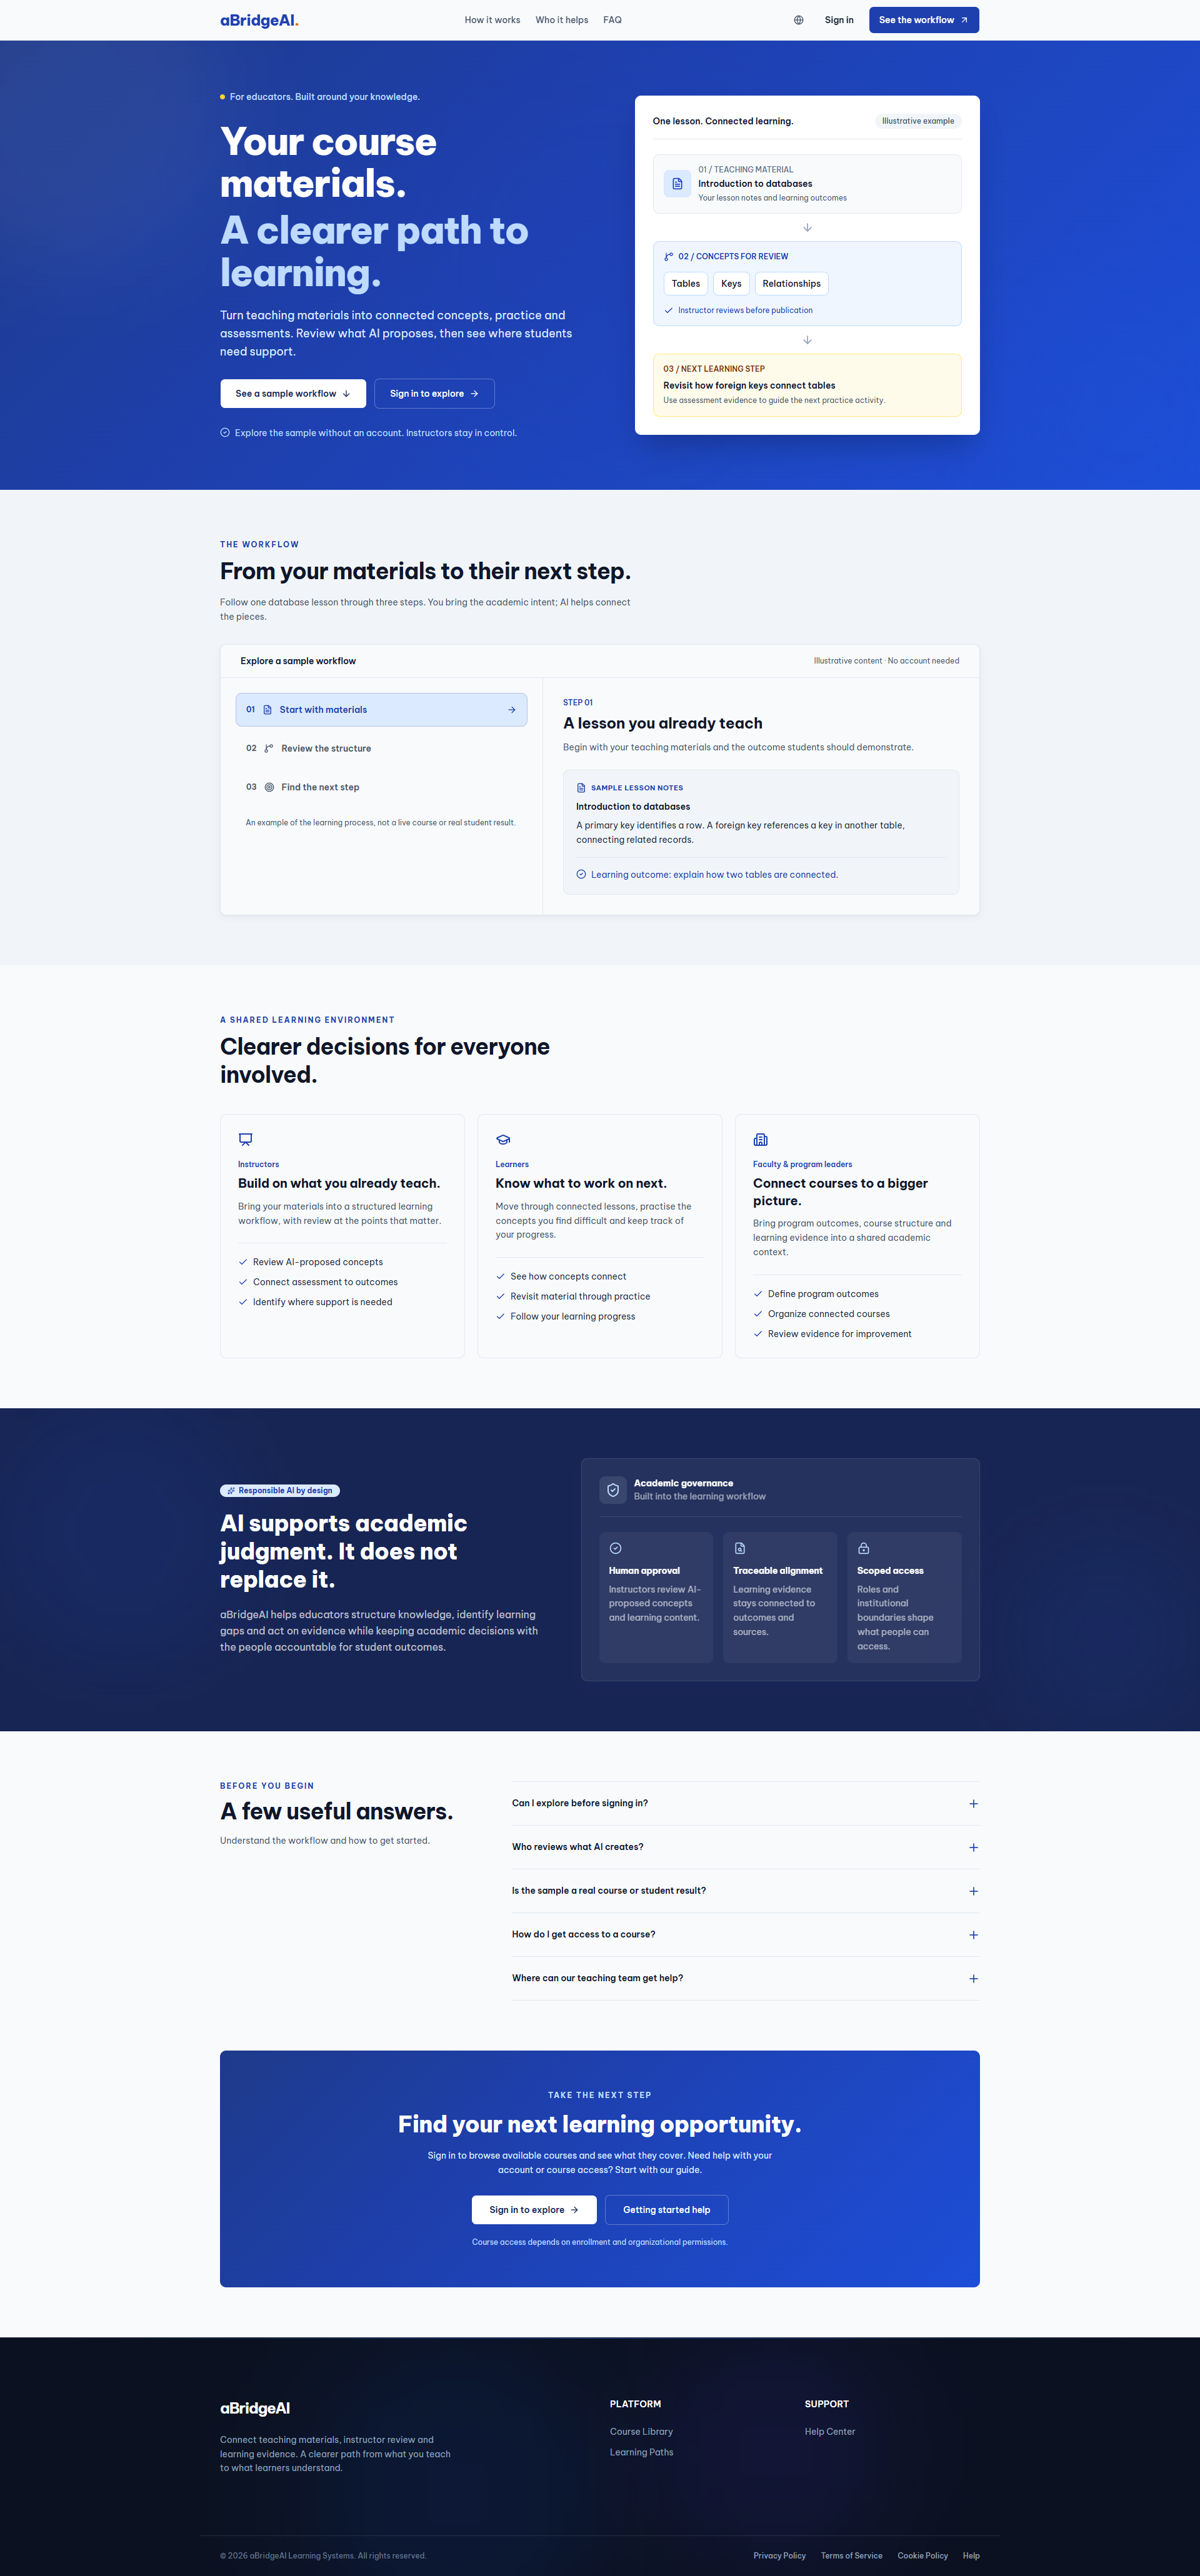
\includegraphics[width=\textwidth,height=0.85\textheight,keepaspectratio]{graphics/screenshots/01_landing_page.png}
  \caption{Landing Page --- Marketing entry point with hero section and call-to-action.}
  \label{fig:landing}
\end{figure}

The landing page is the public marketing surface. It carries a hero headline introducing the AI-powered career-readiness theme, a stats strip, a curated category grid, and a featured-courses carousel. Navigation links to the catalog, login, and sign-up flow are exposed in a horizontal \path|TopNavBar| that is unique to this page. The visual treatment is intentionally distinct from the authenticated shell so that crossing the login boundary feels like a deliberate handoff between marketing and product.

\paragraph{Authentication}

\begin{figure}[H]
  \centering
  \begin{minipage}{0.49\textwidth}
    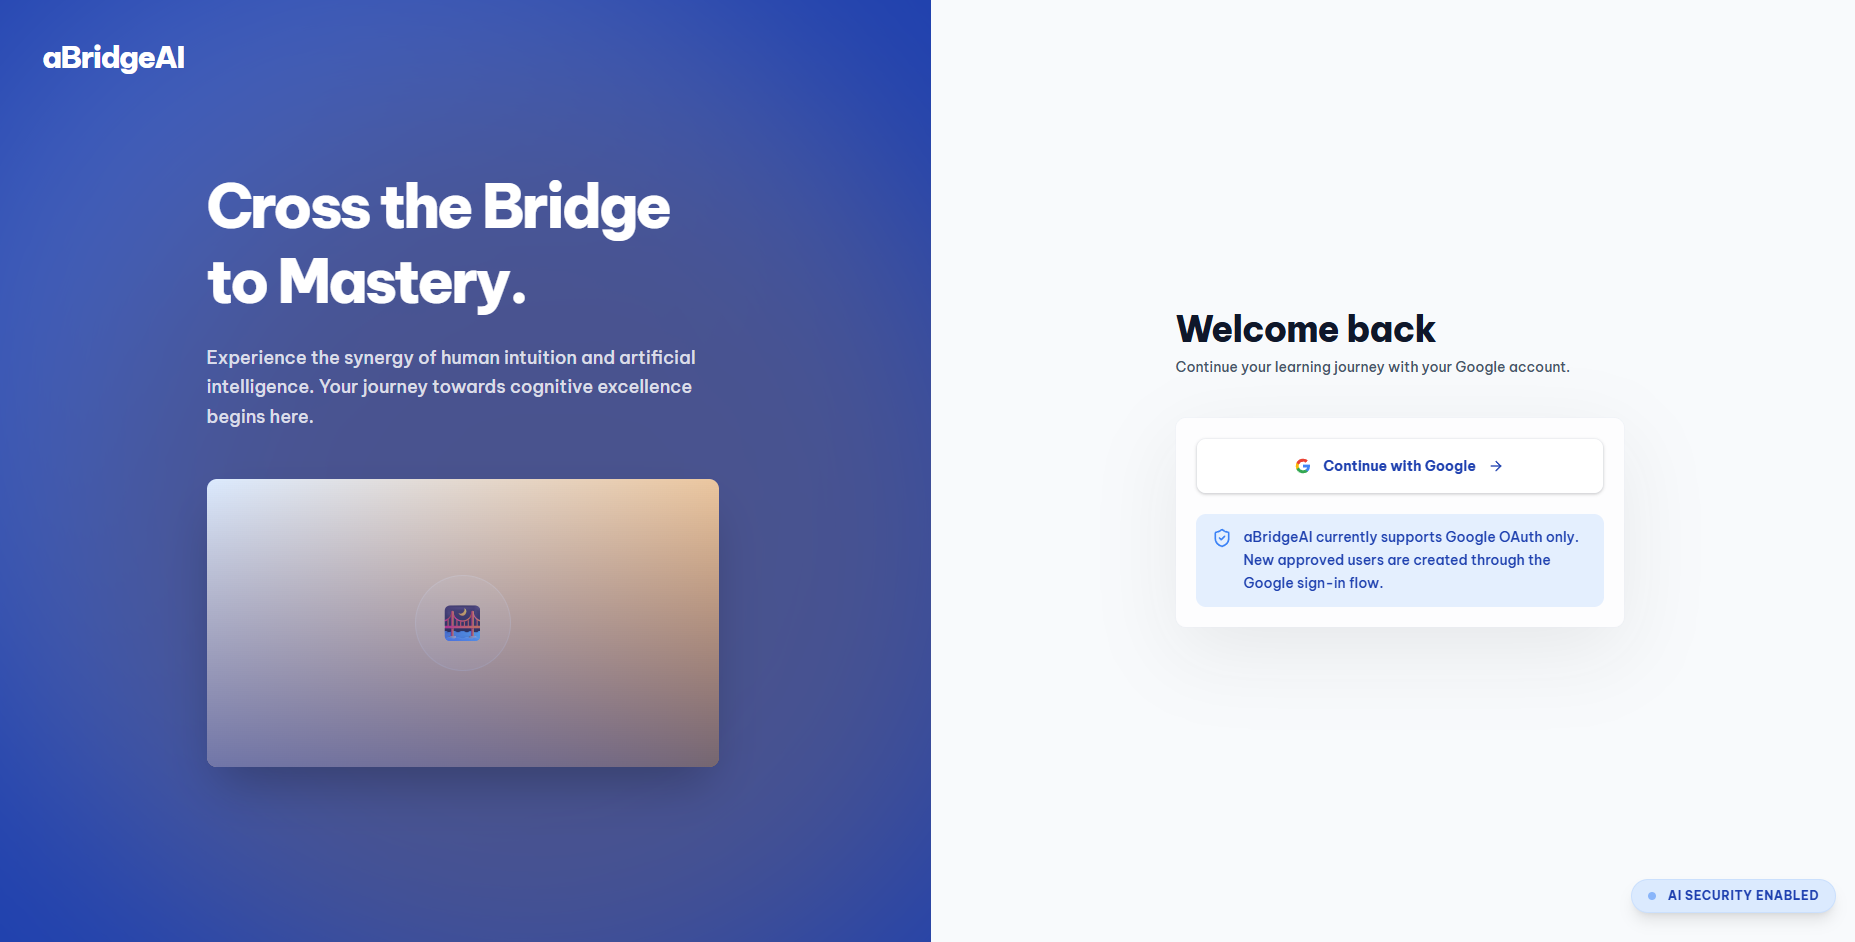
\includegraphics[width=\linewidth]{graphics/screenshots/02_login.png}
    \caption{Login --- Google SSO entry point.}
    \label{fig:login}
  \end{minipage}
\end{figure}

The login screen offers Google SSO as the single sign-in path; on successful redirect, the application checks whether the account has MFA configured and, if so, routes the user to \path|/login/mfa| for a TOTP or recovery-code challenge before issuing a session. A \path|next| query parameter preserves the originally requested route so deep links survive the auth round-trip.

% ── Student ─────────────────────────────────────────────────
\paragraph{Student Dashboard}

\begin{figure}[H]
  \centering
  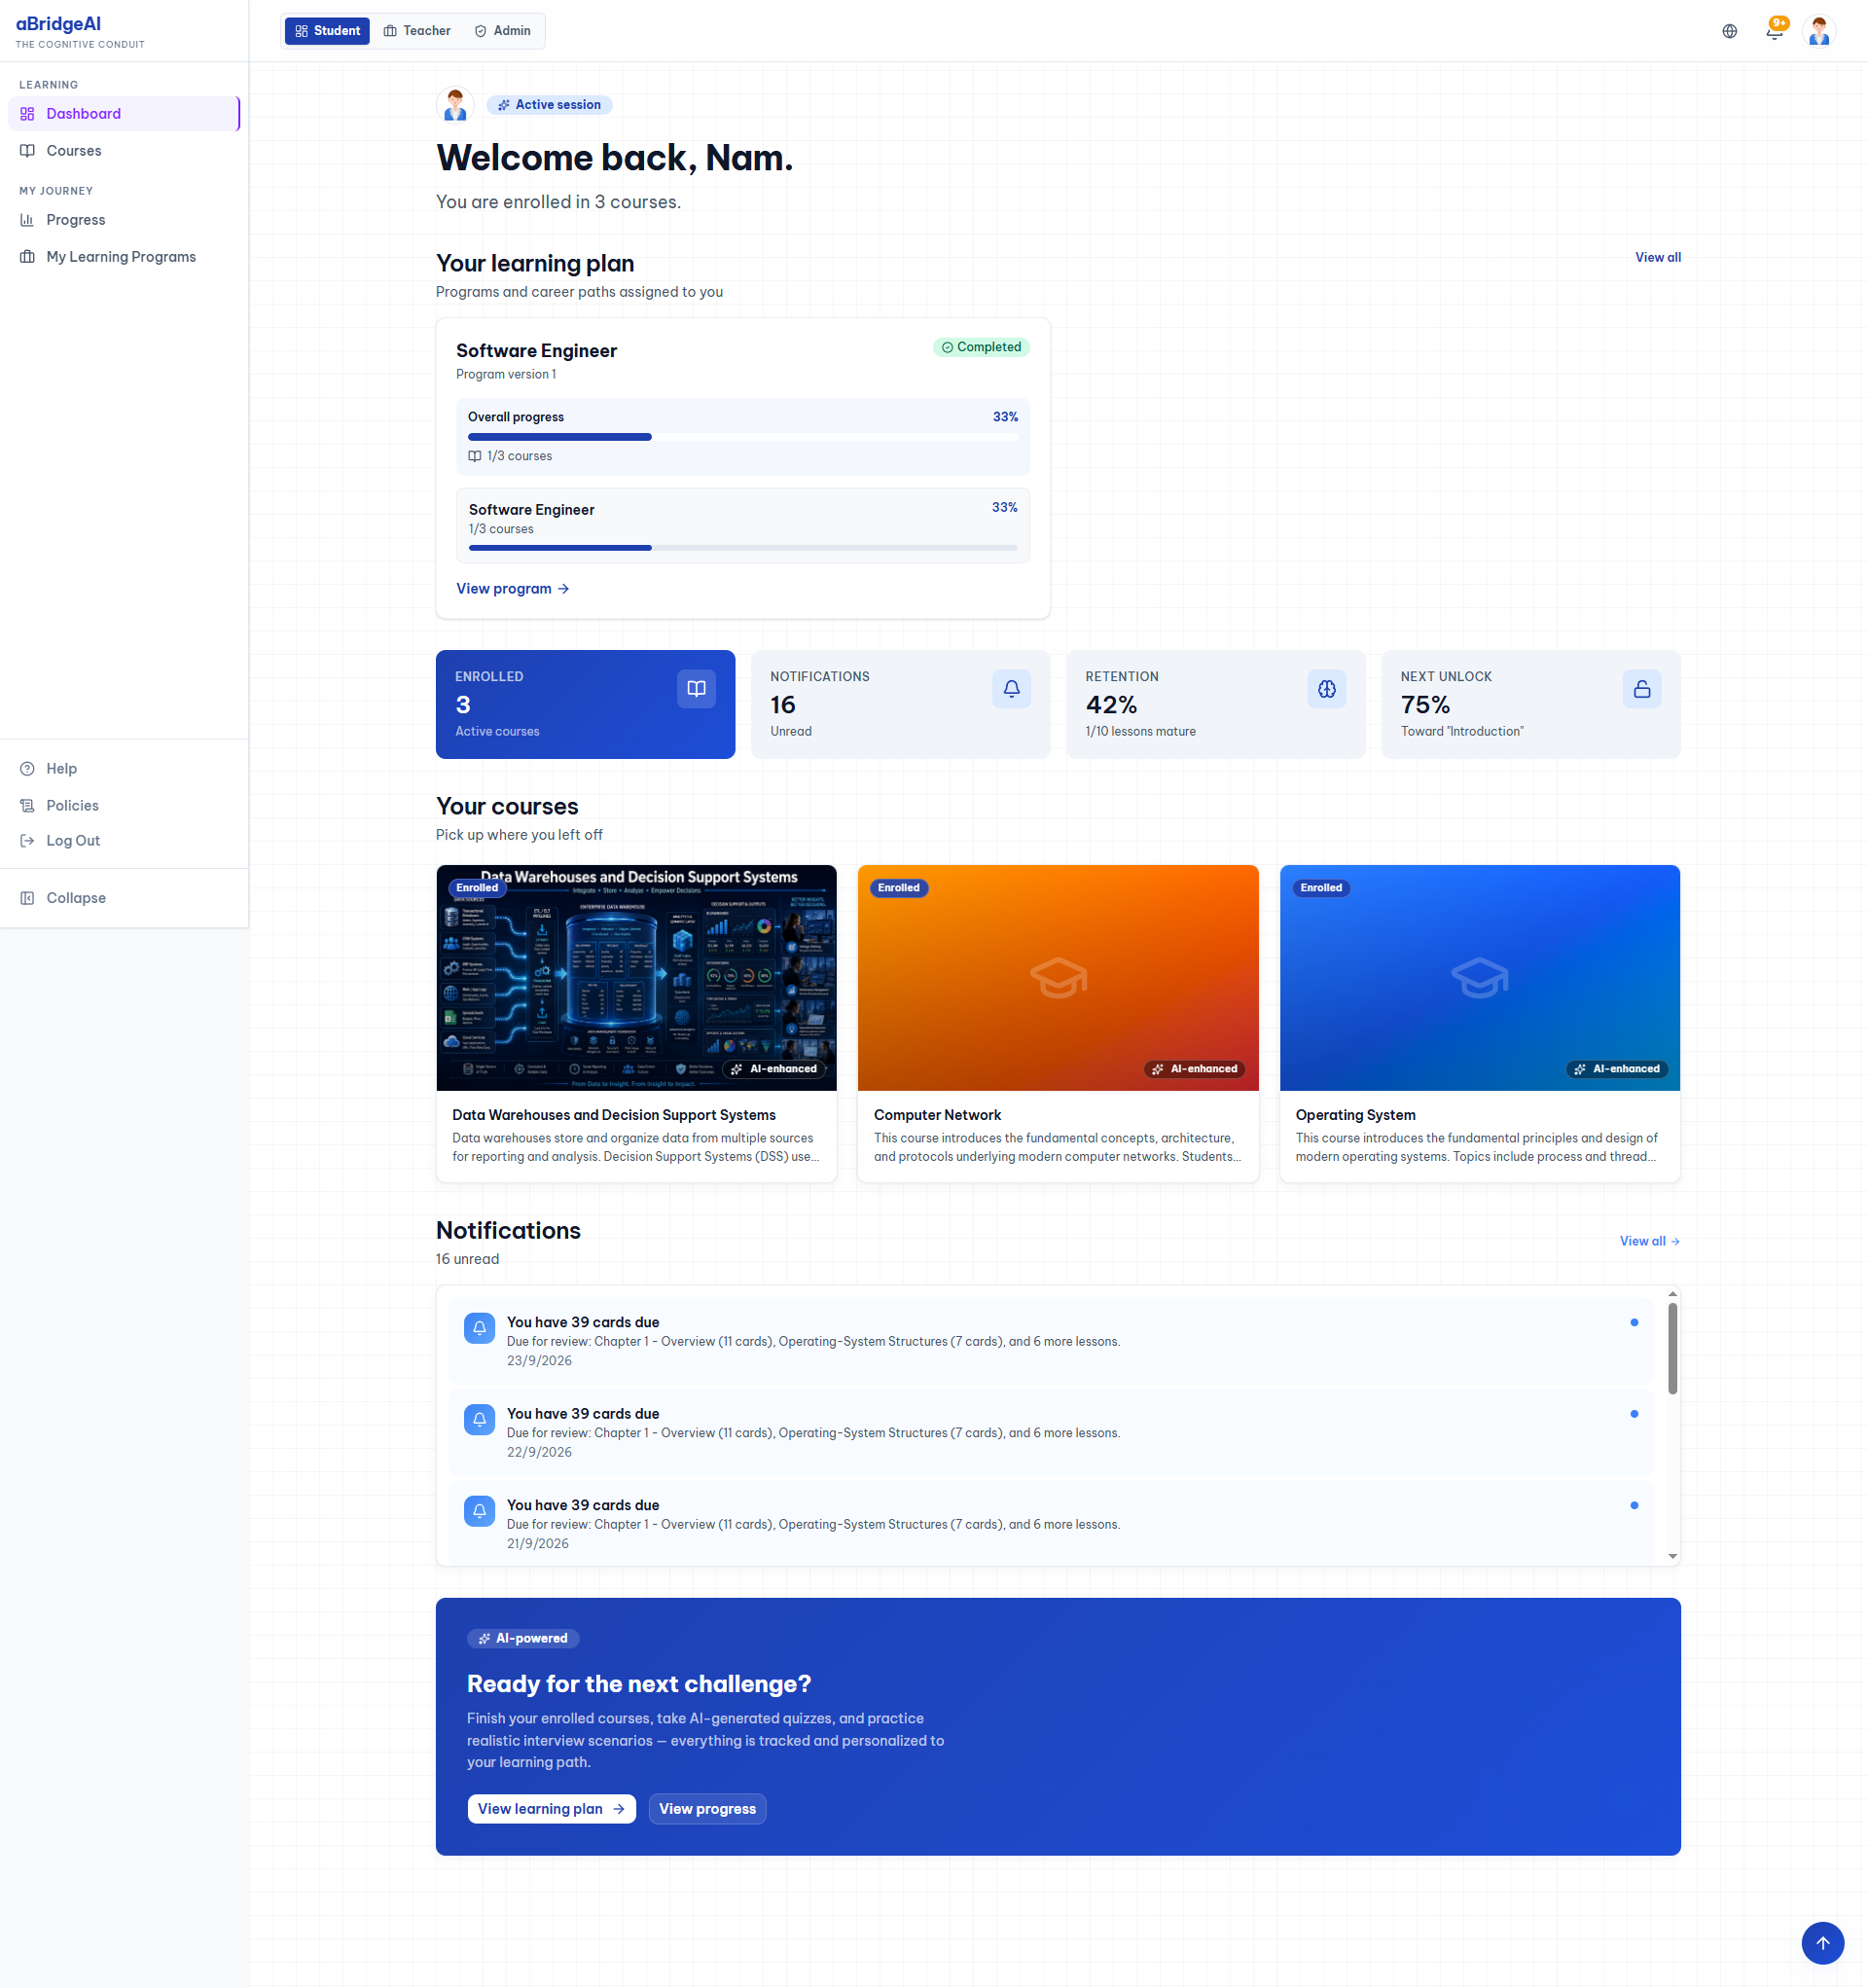
\includegraphics[width=\textwidth]{graphics/screenshots/04_student_dashboard.png}
  \caption{Student Dashboard --- Overview of enrolled courses, due reviews, and recent activity.}
  \label{fig:student_dashboard}
\end{figure}

The student dashboard surfaces only the information needed to decide what to study next. Stat cards summarise enrolled courses, in-progress lessons and recently earned badges; a recommendations strip suggests the next course in the active career path. The layout is intentionally calm --- there is no AI orb or floating action button --- to keep students focused on lesson work rather than ambient prompts.

\paragraph{Course Catalog}

\begin{figure}[H]
  \centering
  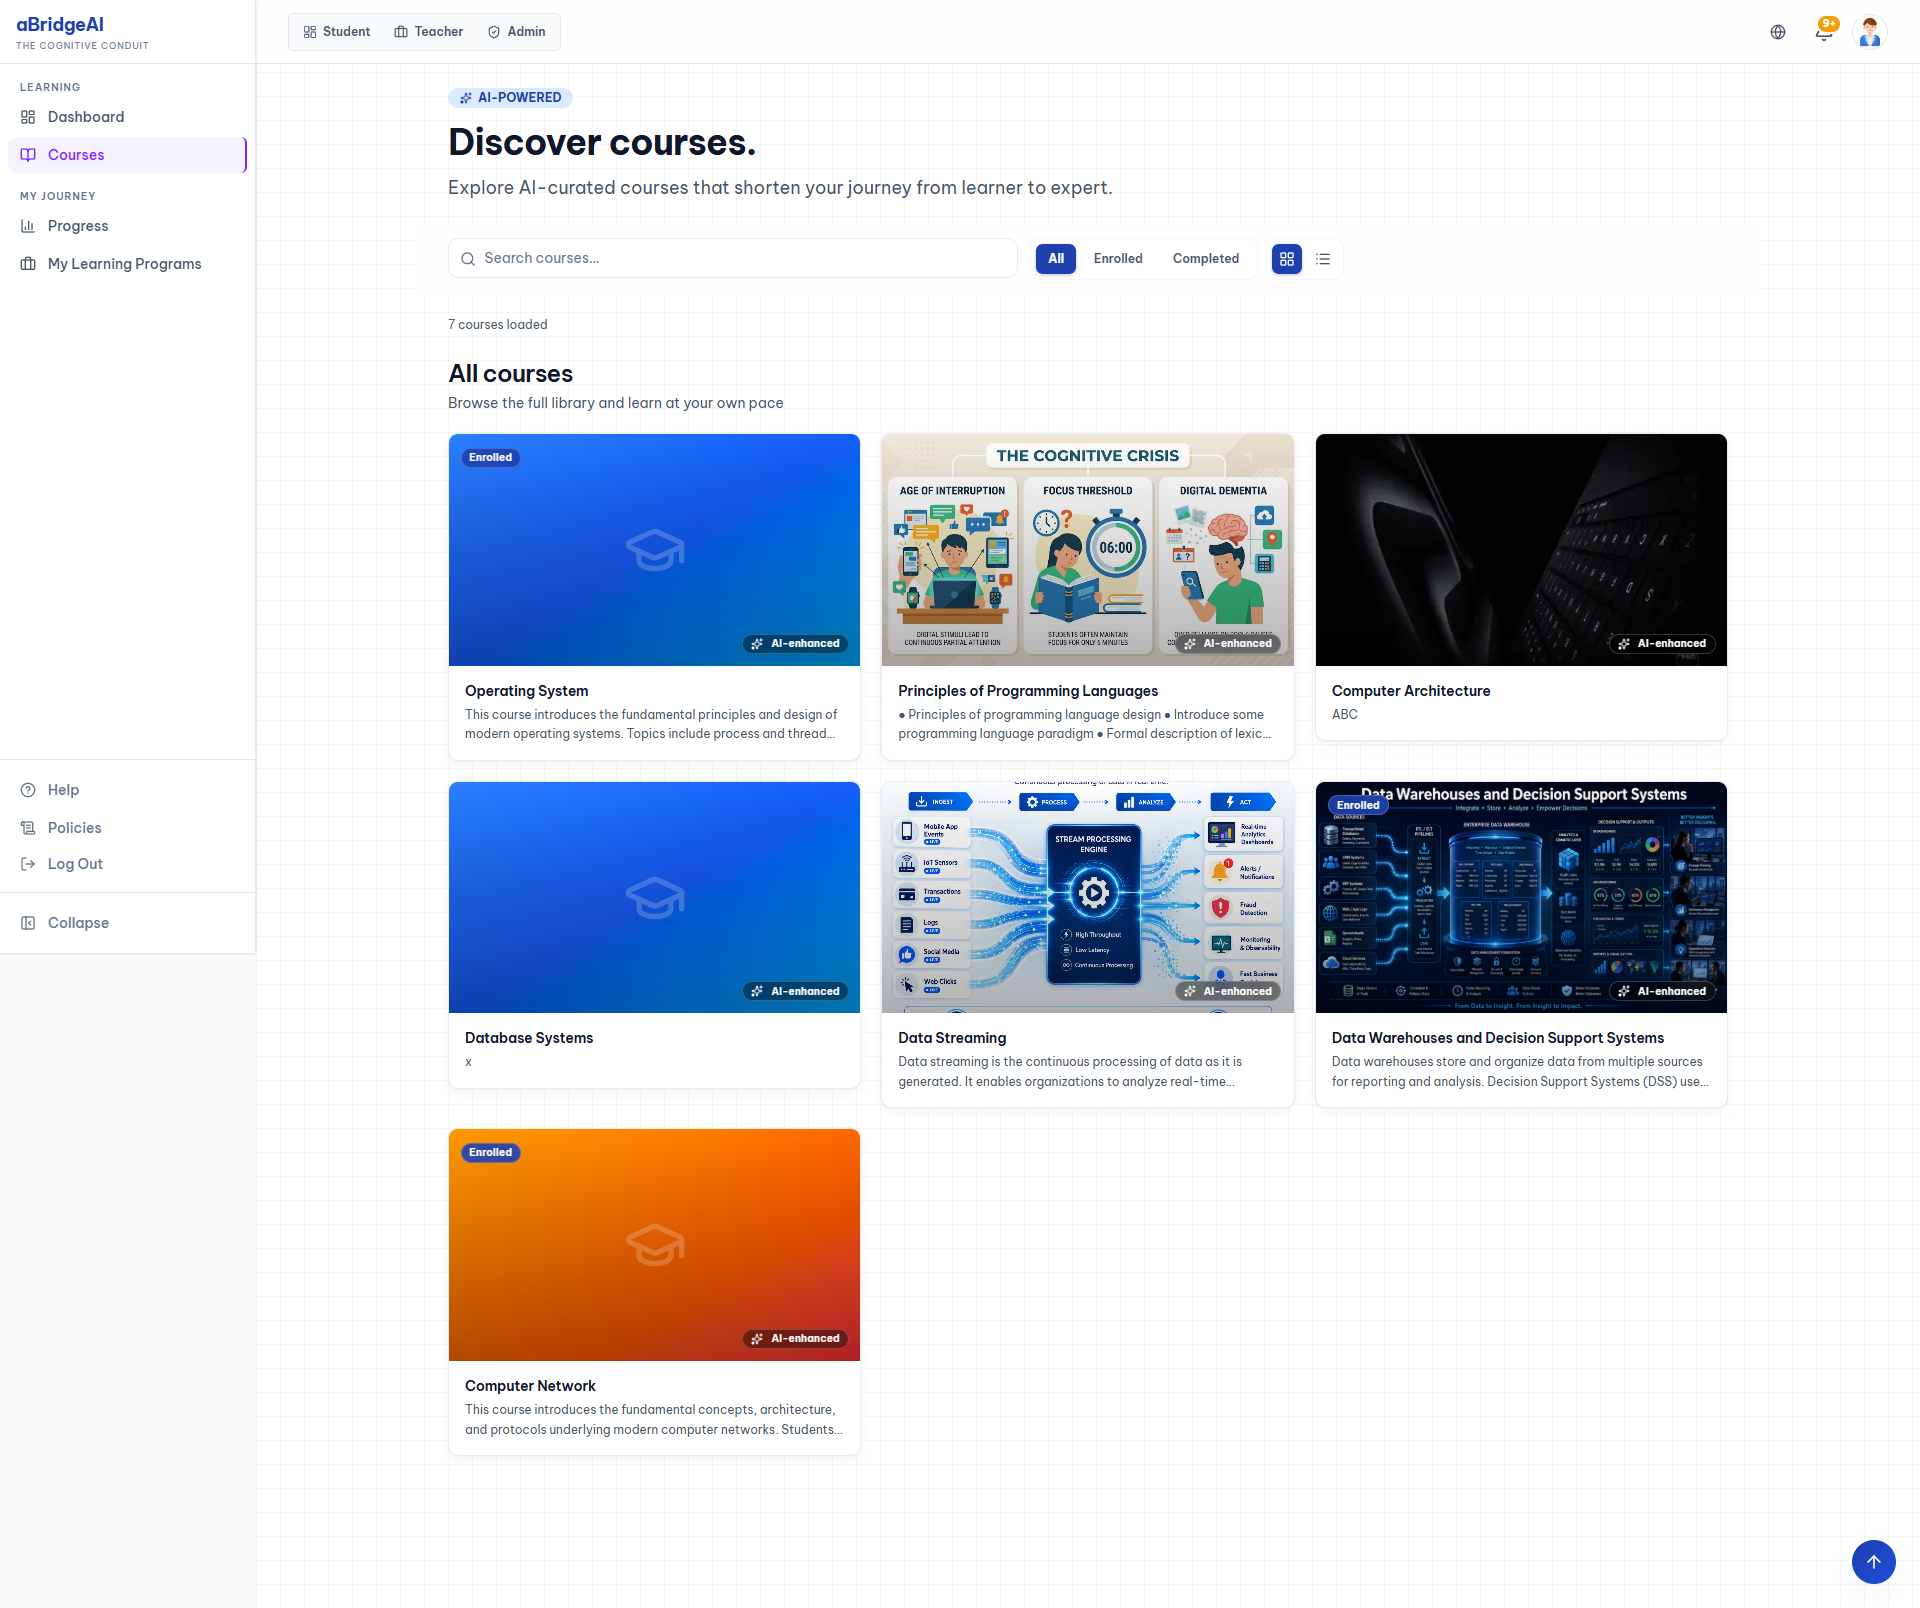
\includegraphics[width=\textwidth]{graphics/screenshots/05_course_catalog.png}
  \caption{Course Catalog --- Search, filter and enrollment status across the full course library.}
  \label{fig:course_catalog}
\end{figure}

The catalog opens with a sticky search and filter bar (query, category, difficulty), followed by a card grid that shows enrollment status and progress inline. Already-enrolled courses display a progress ring so students can pick up where they left off without leaving the catalog page.

\paragraph{Course View}

\begin{figure}[H]
  \centering
  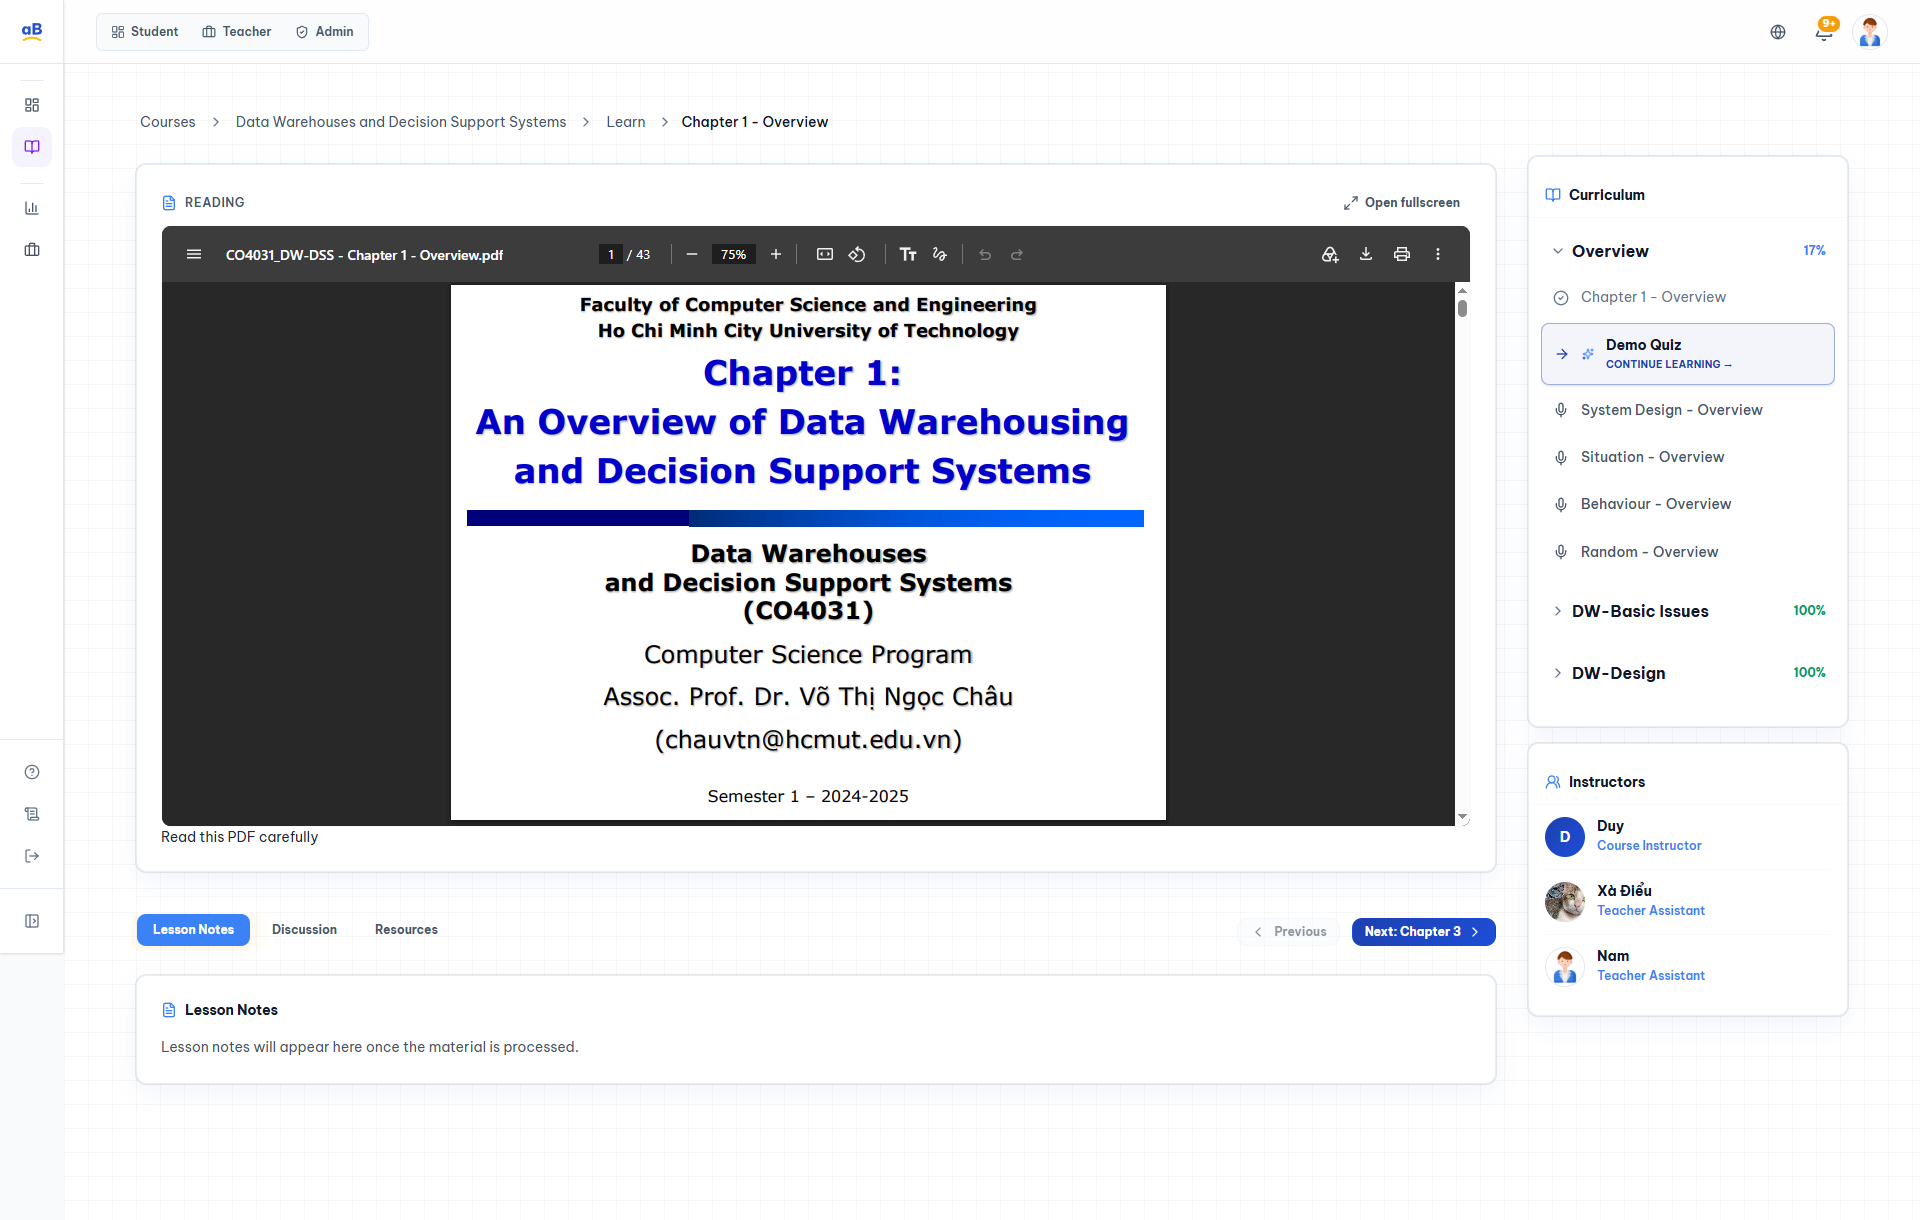
\includegraphics[width=\textwidth]{graphics/screenshots/06_course_view.png}
  \caption{Course View --- Curriculum accordion with lesson state icons.}
  \label{fig:course_view}
\end{figure}

The course view is the primary learning environment. The left panel hosts a sticky progress card and a curriculum accordion; each lesson displays its completion state (completed / active / locked / pending) via iconography. The right panel renders the active lesson's content --- video, reading, attached resources, or an embedded quiz launcher.

\paragraph{Quiz Session}

\begin{figure}[H]
  \centering
  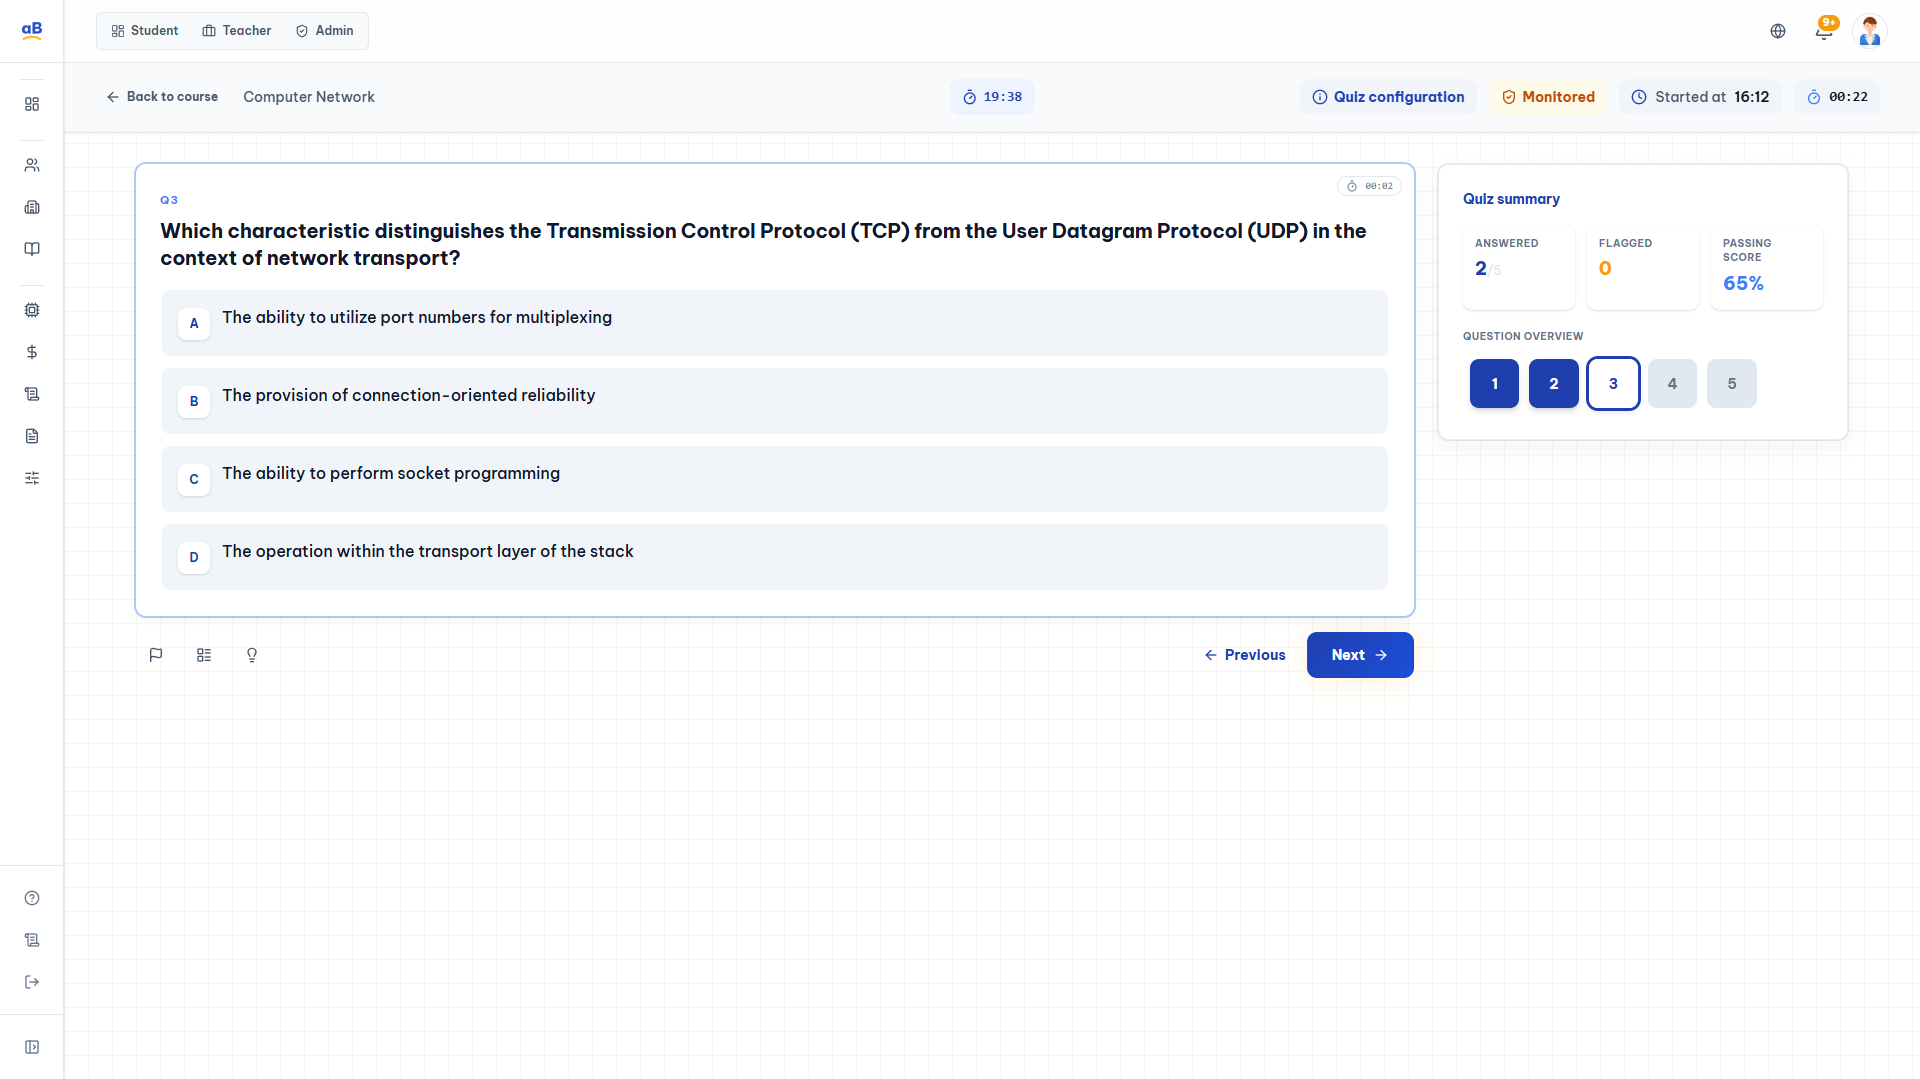
\includegraphics[width=\textwidth]{graphics/screenshots/07_student_quiz.png}
  \caption{Quiz Session --- Timed multiple-choice interface with question navigation.}
  \label{fig:student_quiz}
\end{figure}

The quiz session is a focused, distraction-free interface. A countdown timer at the top creates temporal urgency; the bottom question grid allows non-linear navigation between flagged or unanswered items. After submission, students are redirected to the attempt-review screen at \path|/courses/$slug/quiz/$quizId/attempts/$attemptId|, which renders correct answers and per-question explanations.

% ── Instructor ──────────────────────────────────────────────
\paragraph{Teacher Dashboard}

\begin{figure}[H]
  \centering
  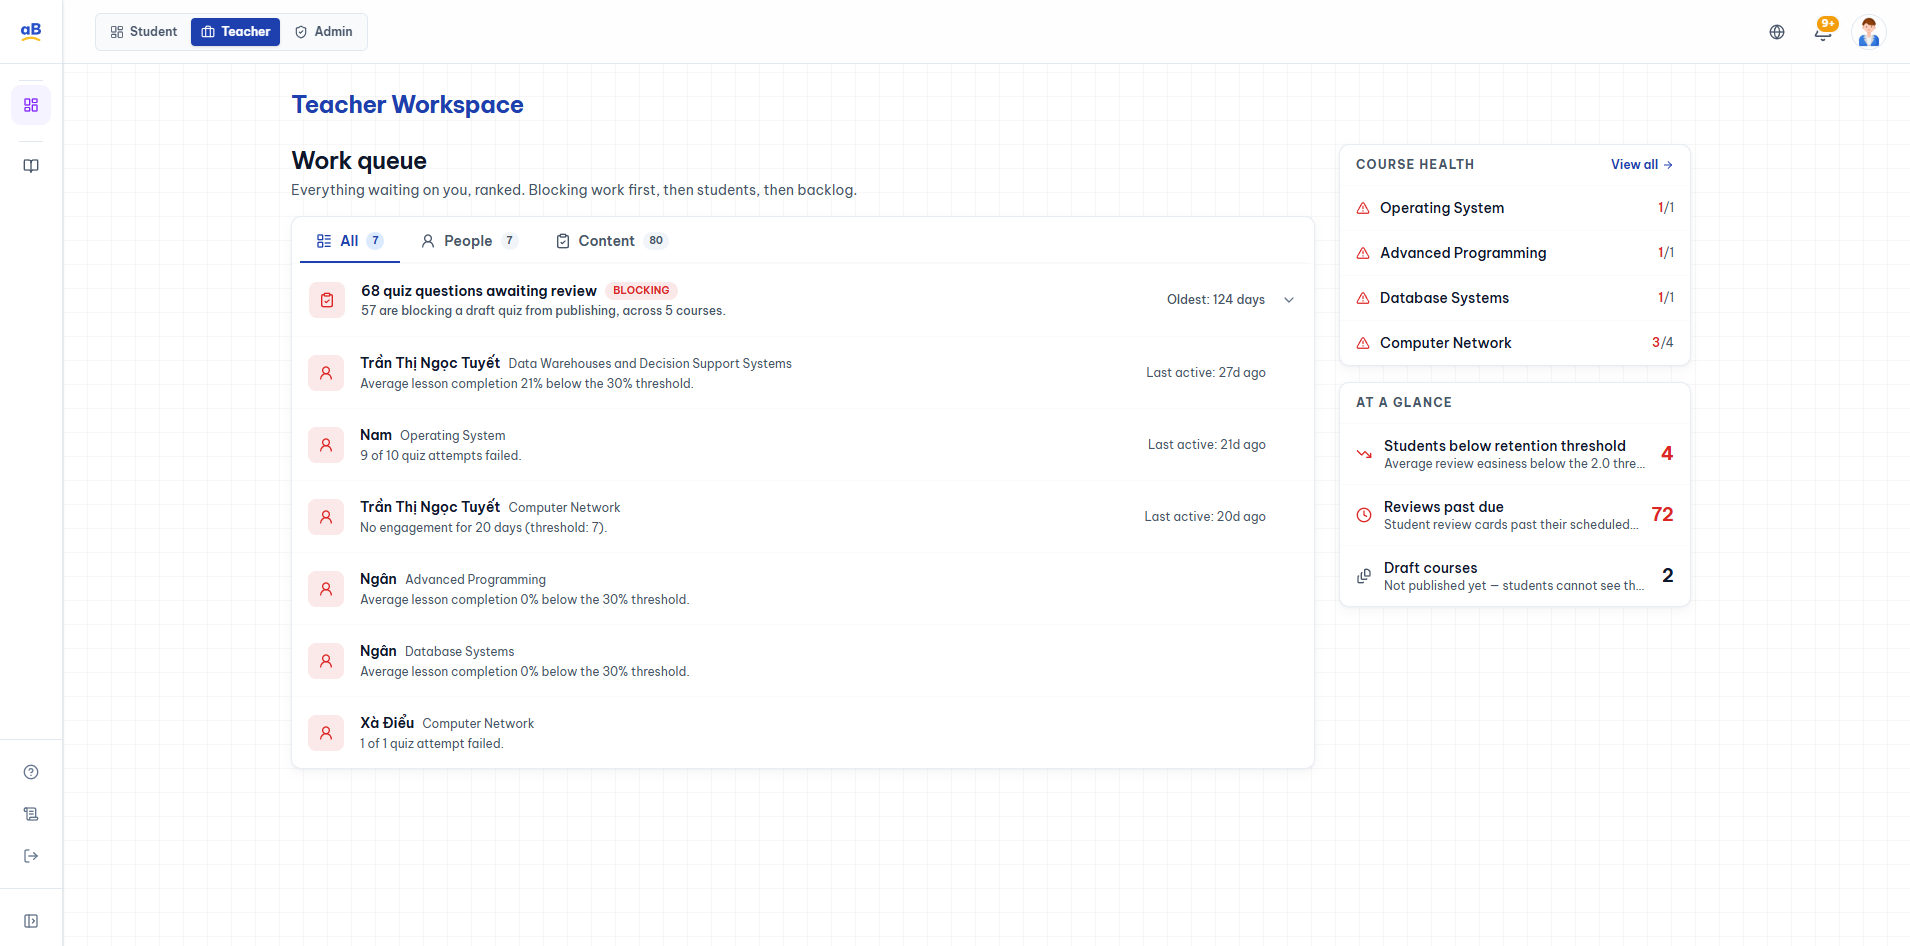
\includegraphics[width=\textwidth]{graphics/screenshots/14_instructor_dashboard.png}
  \caption{Teacher Dashboard --- Operational overview with course health stats and quick course creation.}
  \label{fig:instructor_dashboard}
\end{figure}

The teacher dashboard is the entry screen for the \path|/teacher| route group. Four stat cards summarise the instructor's authoring activity --- total courses, published, drafts, and AI-enabled --- followed by a ``Your Courses'' strip that surfaces the most recently edited course with its difficulty tag and publish state. A primary \textbf{+ New Course} button anchors the top-right corner, and a \textbf{Manage} link on each course card jumps directly into the course-management view. The role switcher (Student / Teacher / Admin) at the top of the page is a development affordance for users that hold multiple roles; production accounts only see the tabs they are entitled to.

\paragraph{Course Management}

\begin{figure}[H]
  \centering
  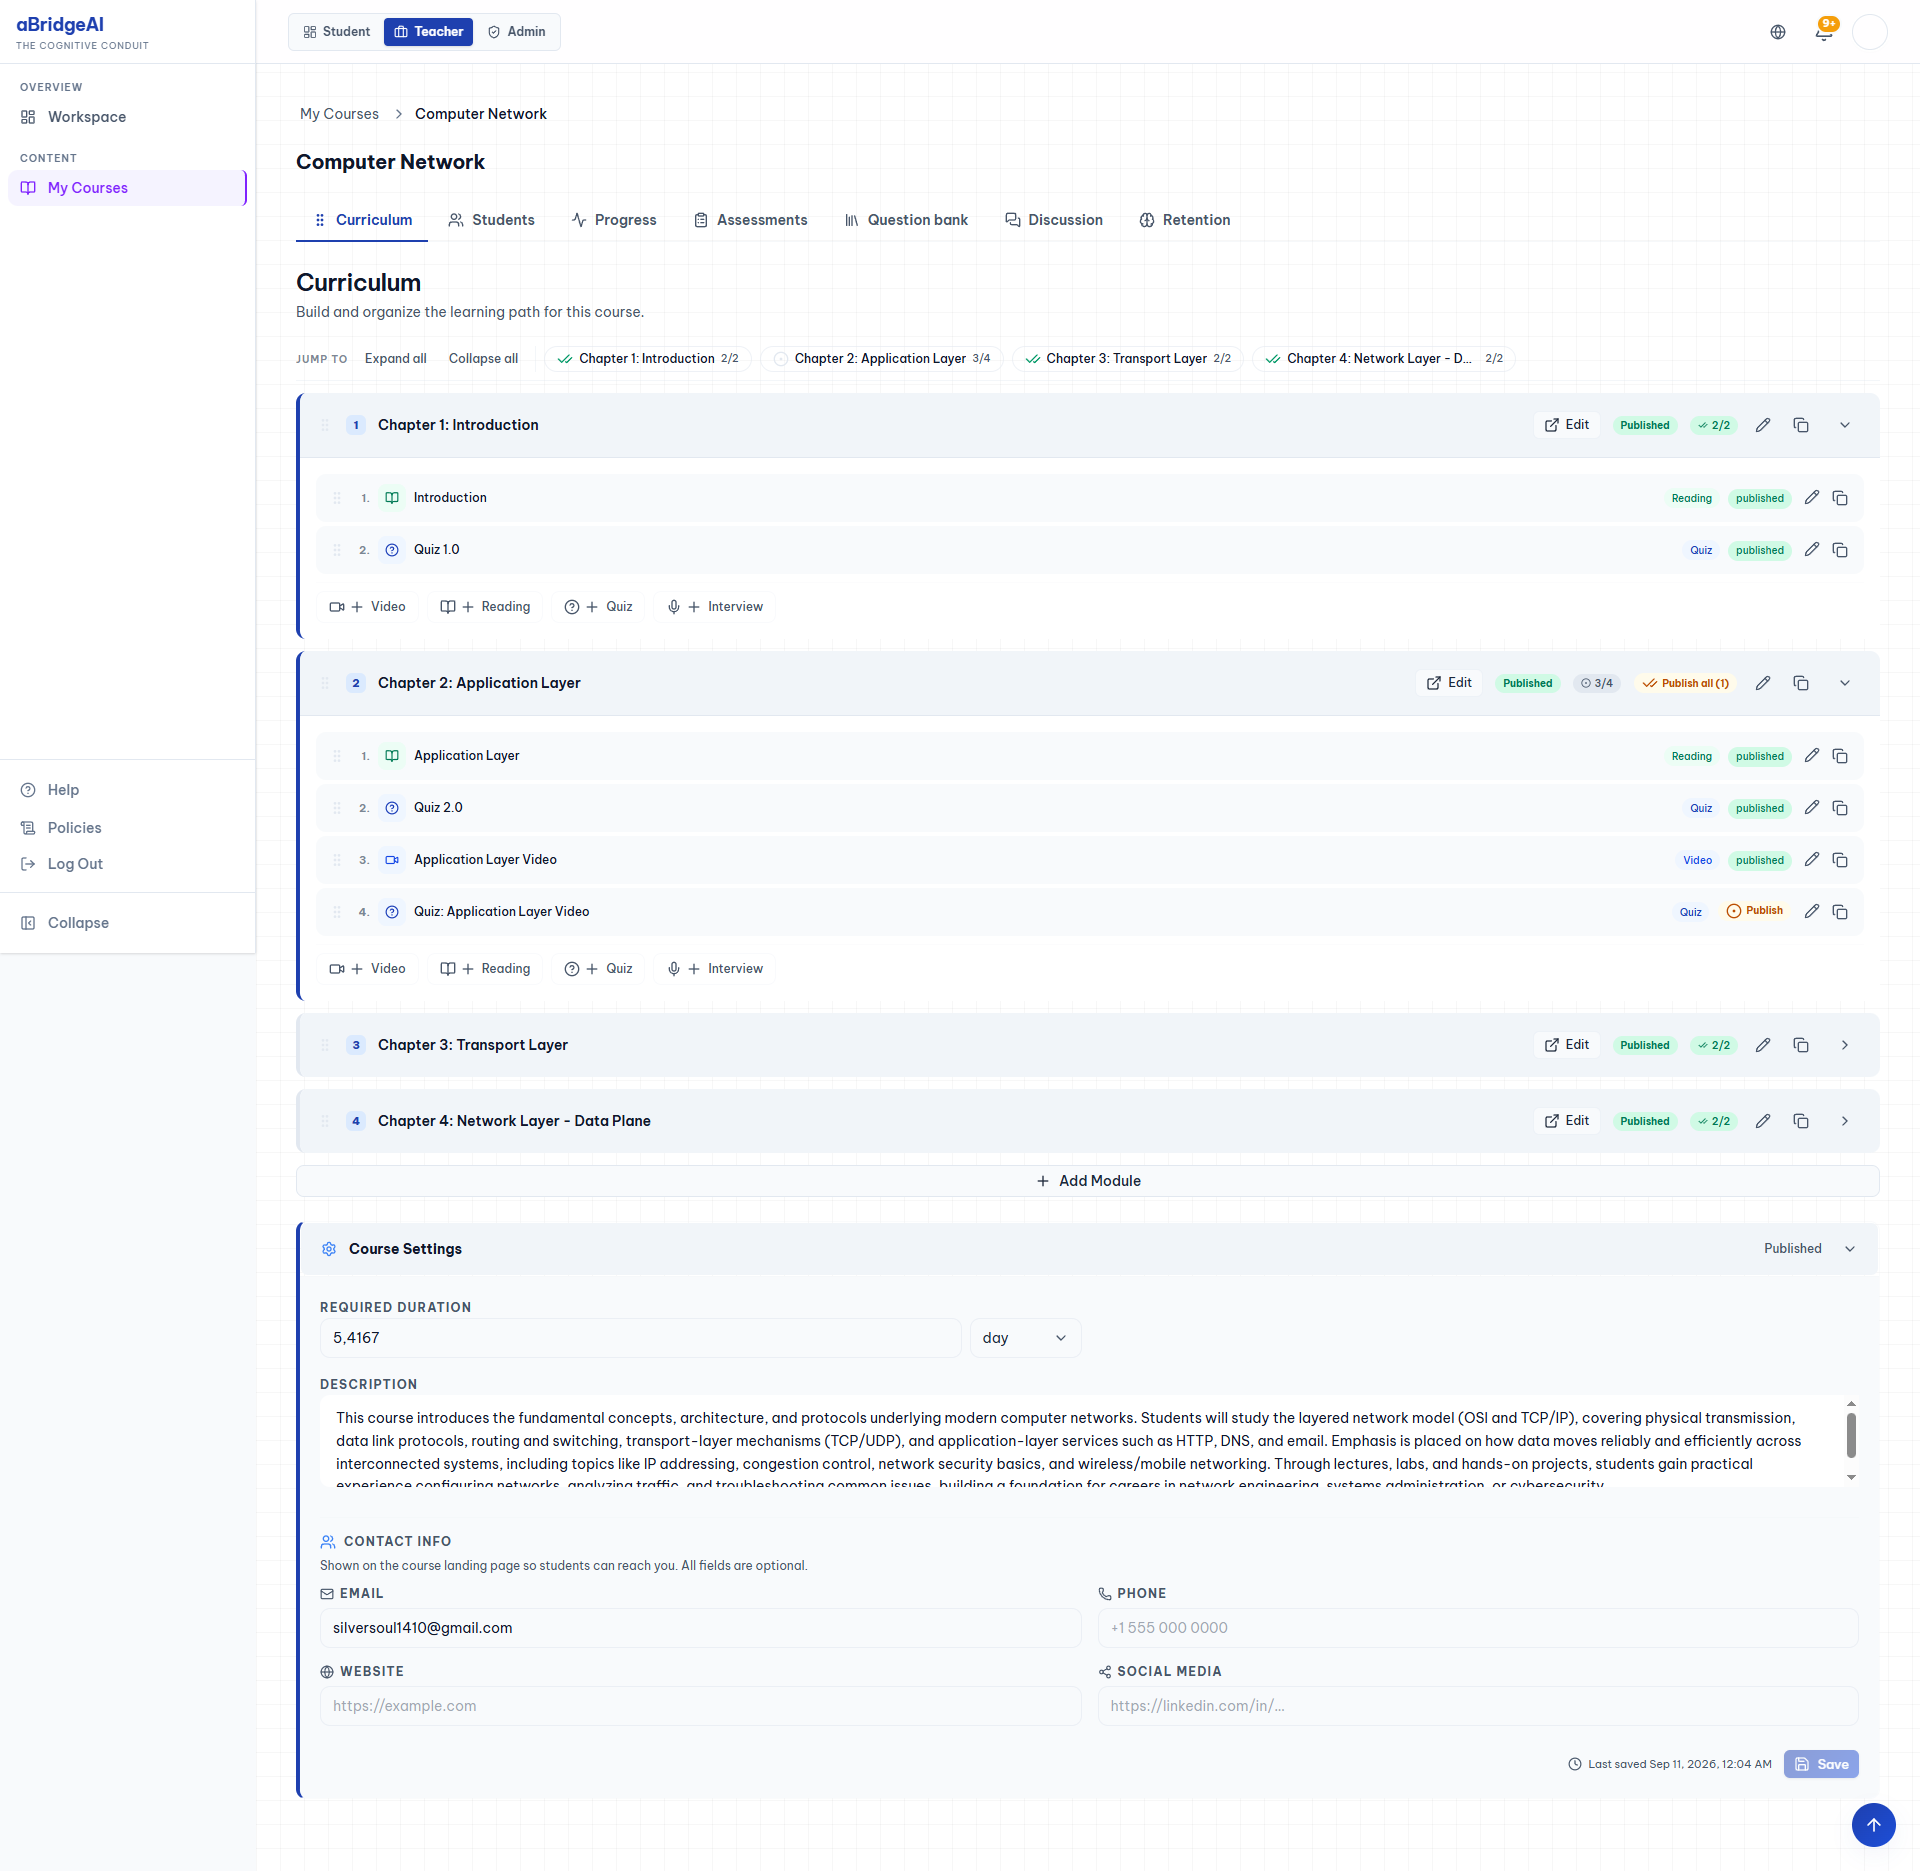
\includegraphics[width=\textwidth]{graphics/screenshots/instructor_course_manage.png}
  \caption{Course Manage --- Module and lesson tree with drag-handle reordering and inline quick-add.}
  \label{fig:instructor_course_manage}
\end{figure}

The course-management page (\path|/teacher/courses/$courseId|) is the authoring core of the platform. Modules render as collapsible cards in a drag-handle list; expanding a module reveals its ordered lesson and quiz items, each carrying a publish-state badge. Inline \textbf{+ Video}, \textbf{+ Reading} and \textbf{+ Quiz} buttons let the instructor grow the curriculum without leaving the page. A right-hand \textit{Course Settings} panel exposes the publish toggle, difficulty, and Students / Progress / Manage Enrollments quick links. A bottom \textbf{+ Add Module} button extends the structure.

\paragraph{Lesson Editor}

\begin{figure}[H]
  \centering
  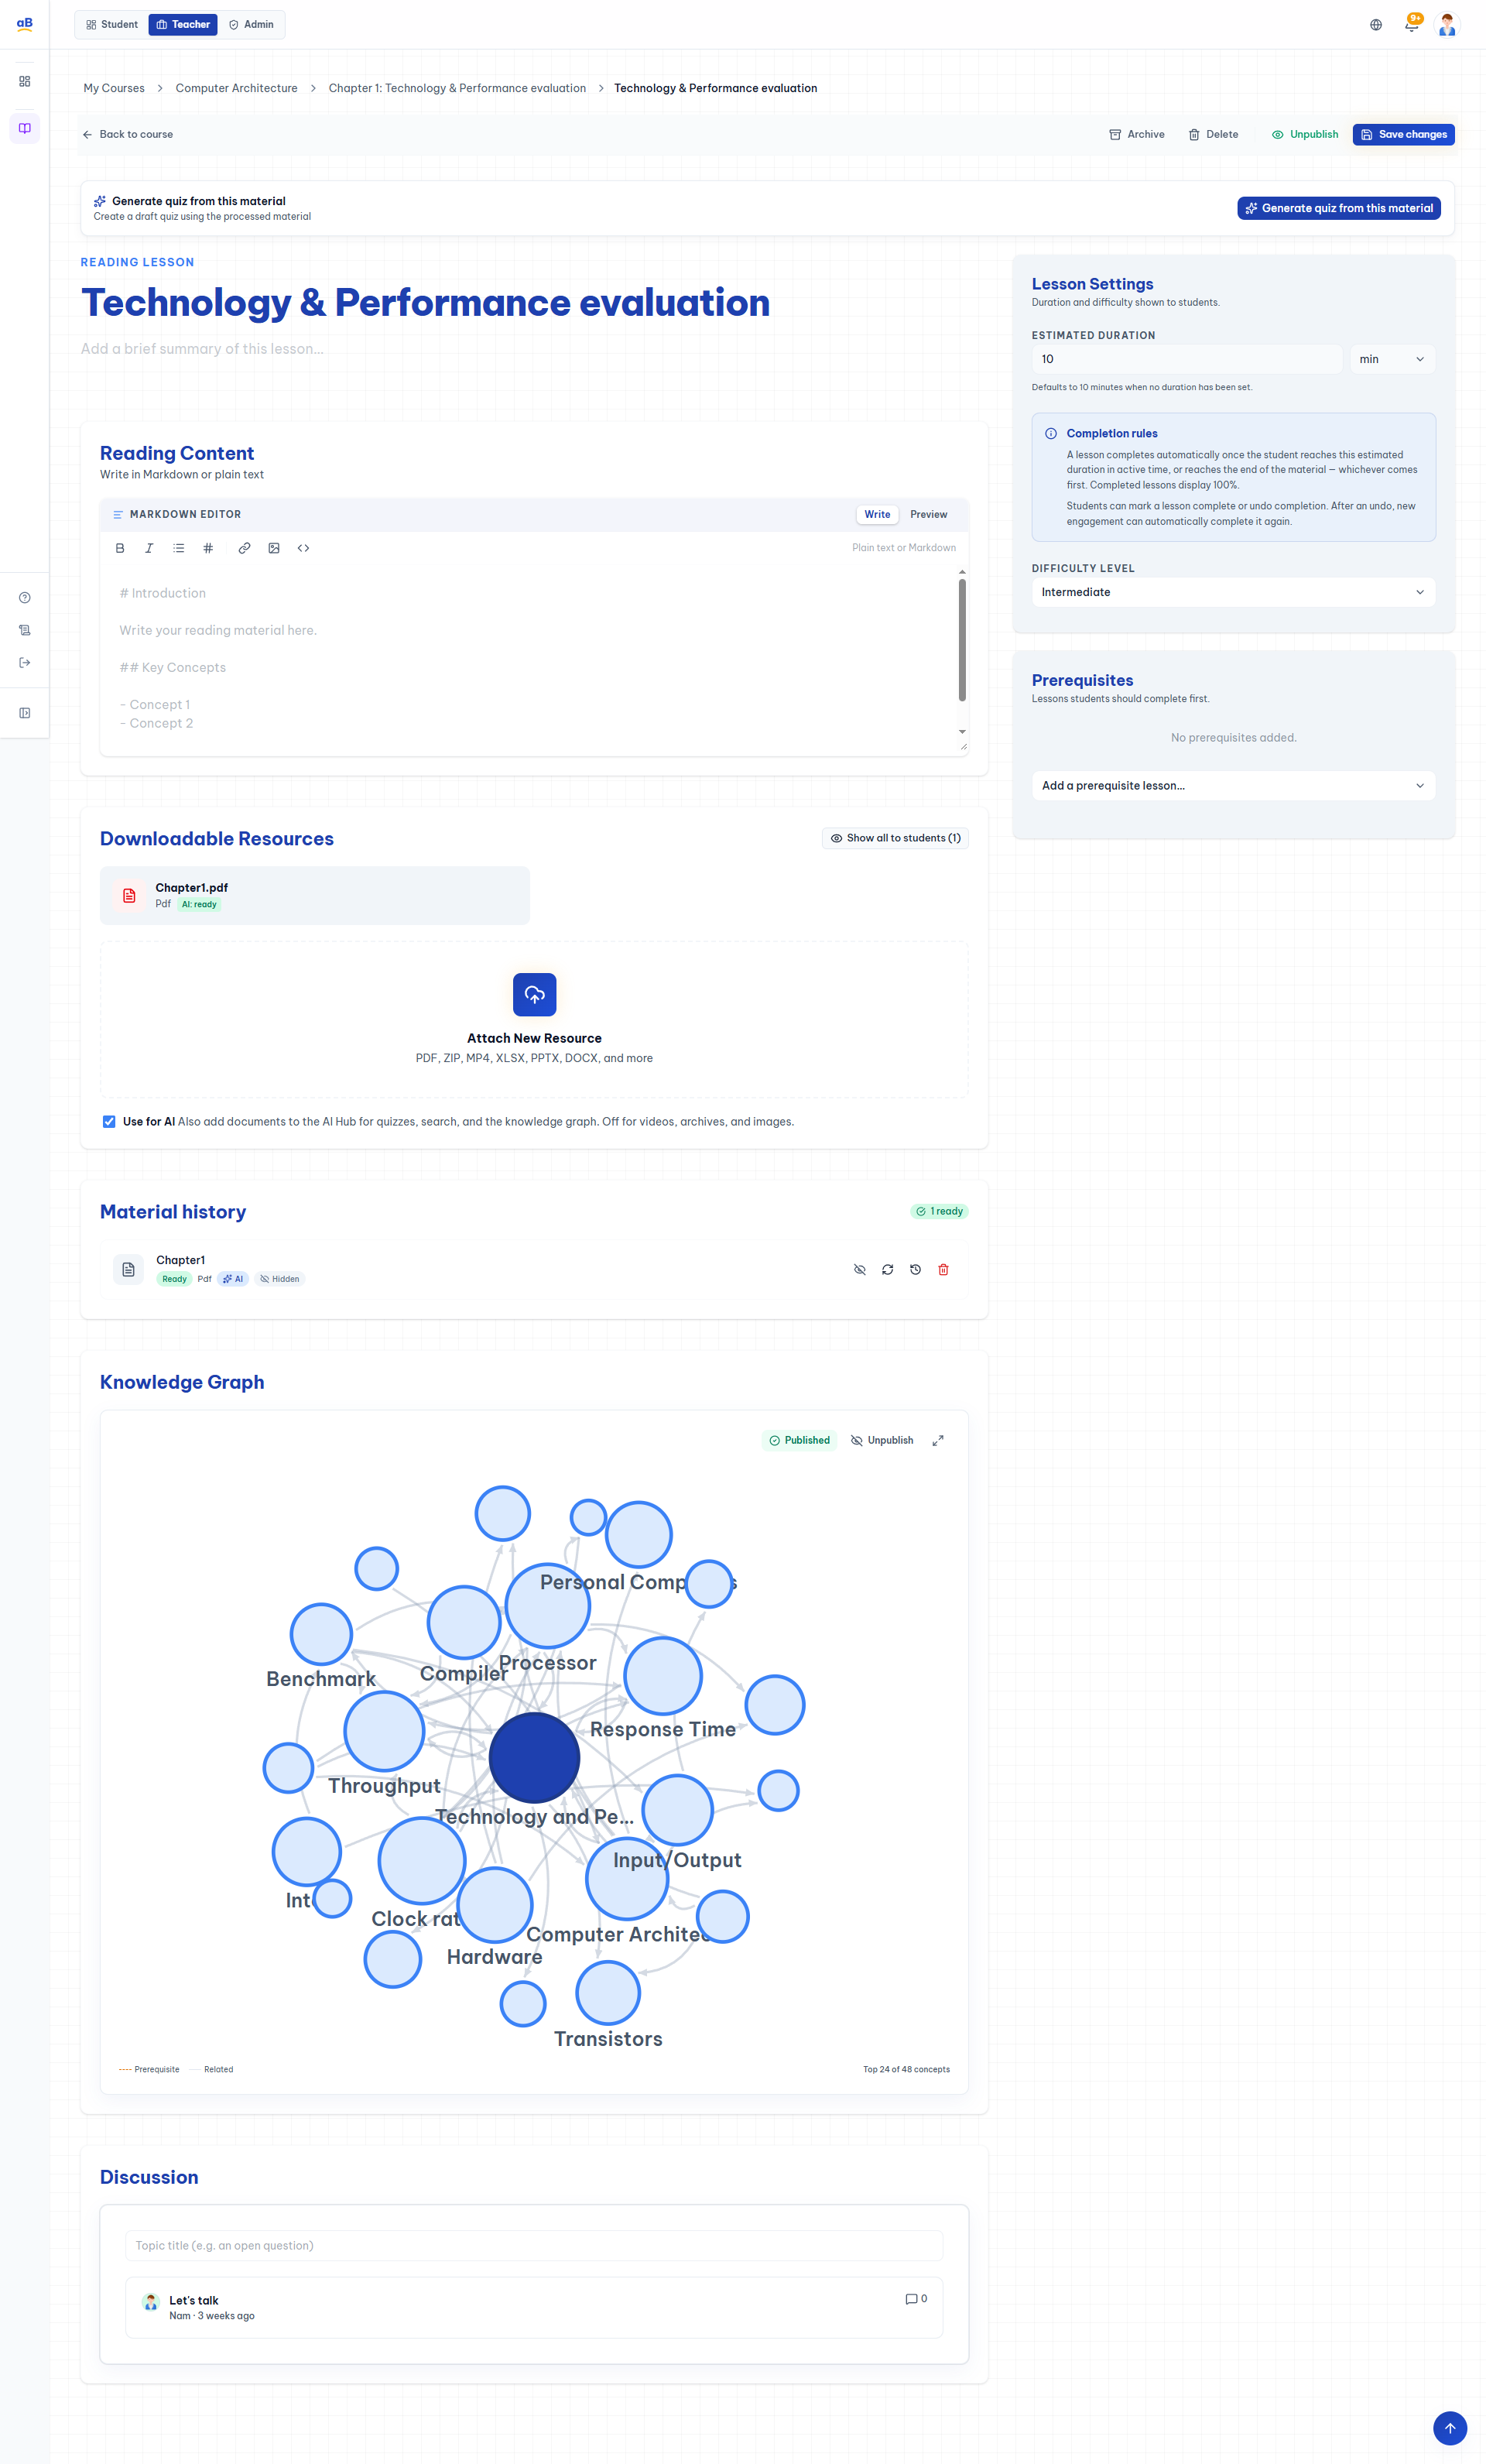
\includegraphics[width=\textwidth]{graphics/screenshots/instructor_lesson_manage.png}
  \caption{Lesson Editor --- Markdown content editor with attached resources and right-hand settings panel.}
  \label{fig:instructor_lesson_manage}
\end{figure}

The lesson editor (\path|/teacher/courses/$courseId/lessons/$lessonId|) is split into a content area and a settings sidebar. The left side shows a Markdown editor for reading lessons (with bold, italic, list, heading, link, image, and code controls) and a \textit{Downloadable Resources} block for attached PDFs and other files. The right sidebar exposes Visibility (Published / Draft), Lesson Type (Video / Reading), Estimated Duration, Difficulty Level, and a Prerequisites picker. An \textit{AI Material Hub} card promotes uploading source material so the platform can auto-generate quizzes from it. Destructive actions (Archive, Delete) are pushed to the bottom of the sidebar to reduce mis-clicks. A persistent \textbf{Save changes} button anchors the top-right corner.

\paragraph{Quiz Editor}

\begin{figure}[H]
  \centering
  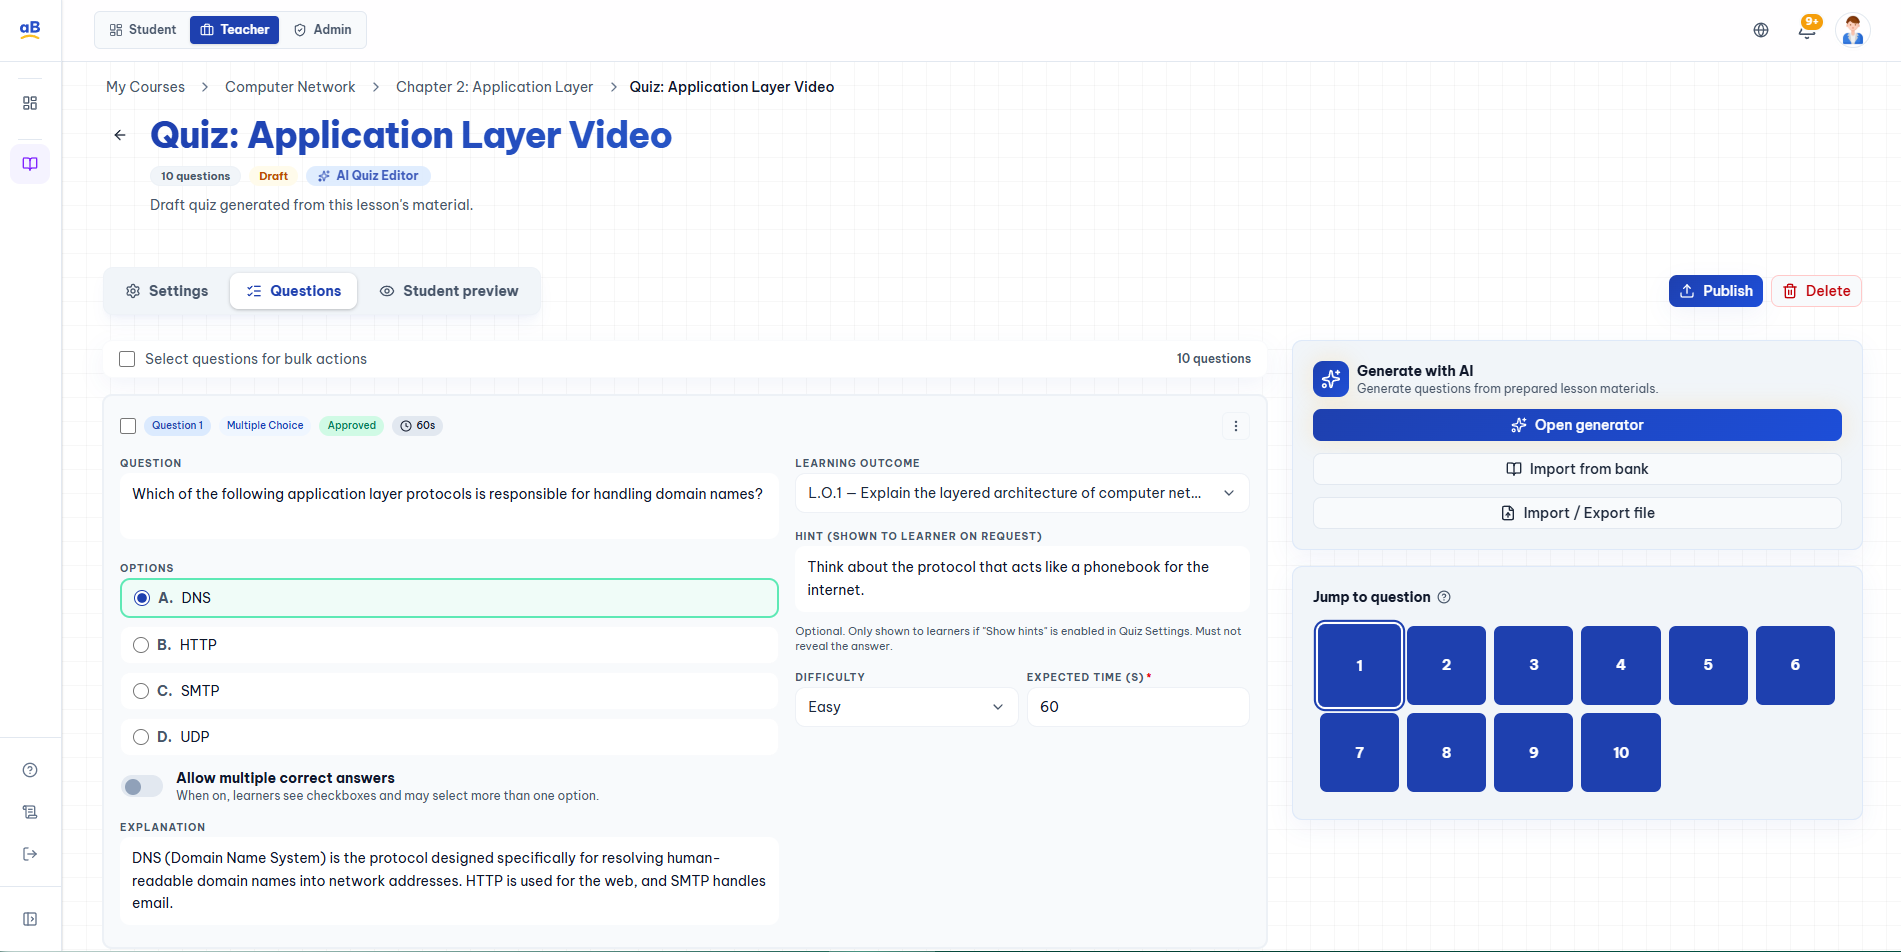
\includegraphics[width=\textwidth]{graphics/screenshots/24_quiz_editor.png}
  \caption{Quiz Editor --- Question list with bulk timing controls and an AI-generation side panel.}
  \label{fig:instructor_quiz_editor}
\end{figure}

The quiz editor (\path|/teacher/courses/$courseId/quizzes/$quizId|) is structured around three sub-tabs: \textbf{Questions} (active by default), \textbf{Settings}, and \textbf{Preview}. The Questions tab lists every item with its type badge (Multiple Choice, True/False, \dots), per-question time limit, and approval status. A bulk-action toolbar lets instructors select multiple questions and apply a uniform time limit, approve in bulk, or delete. A persistent banner reports how many questions are pending review (e.g.\ ``74 questions are pending review --- approve them before publishing''), enforcing a deliberate approval gate between AI generation and student exposure.

\paragraph{AI Quiz Generation}

\begin{figure}[H]
  \centering
  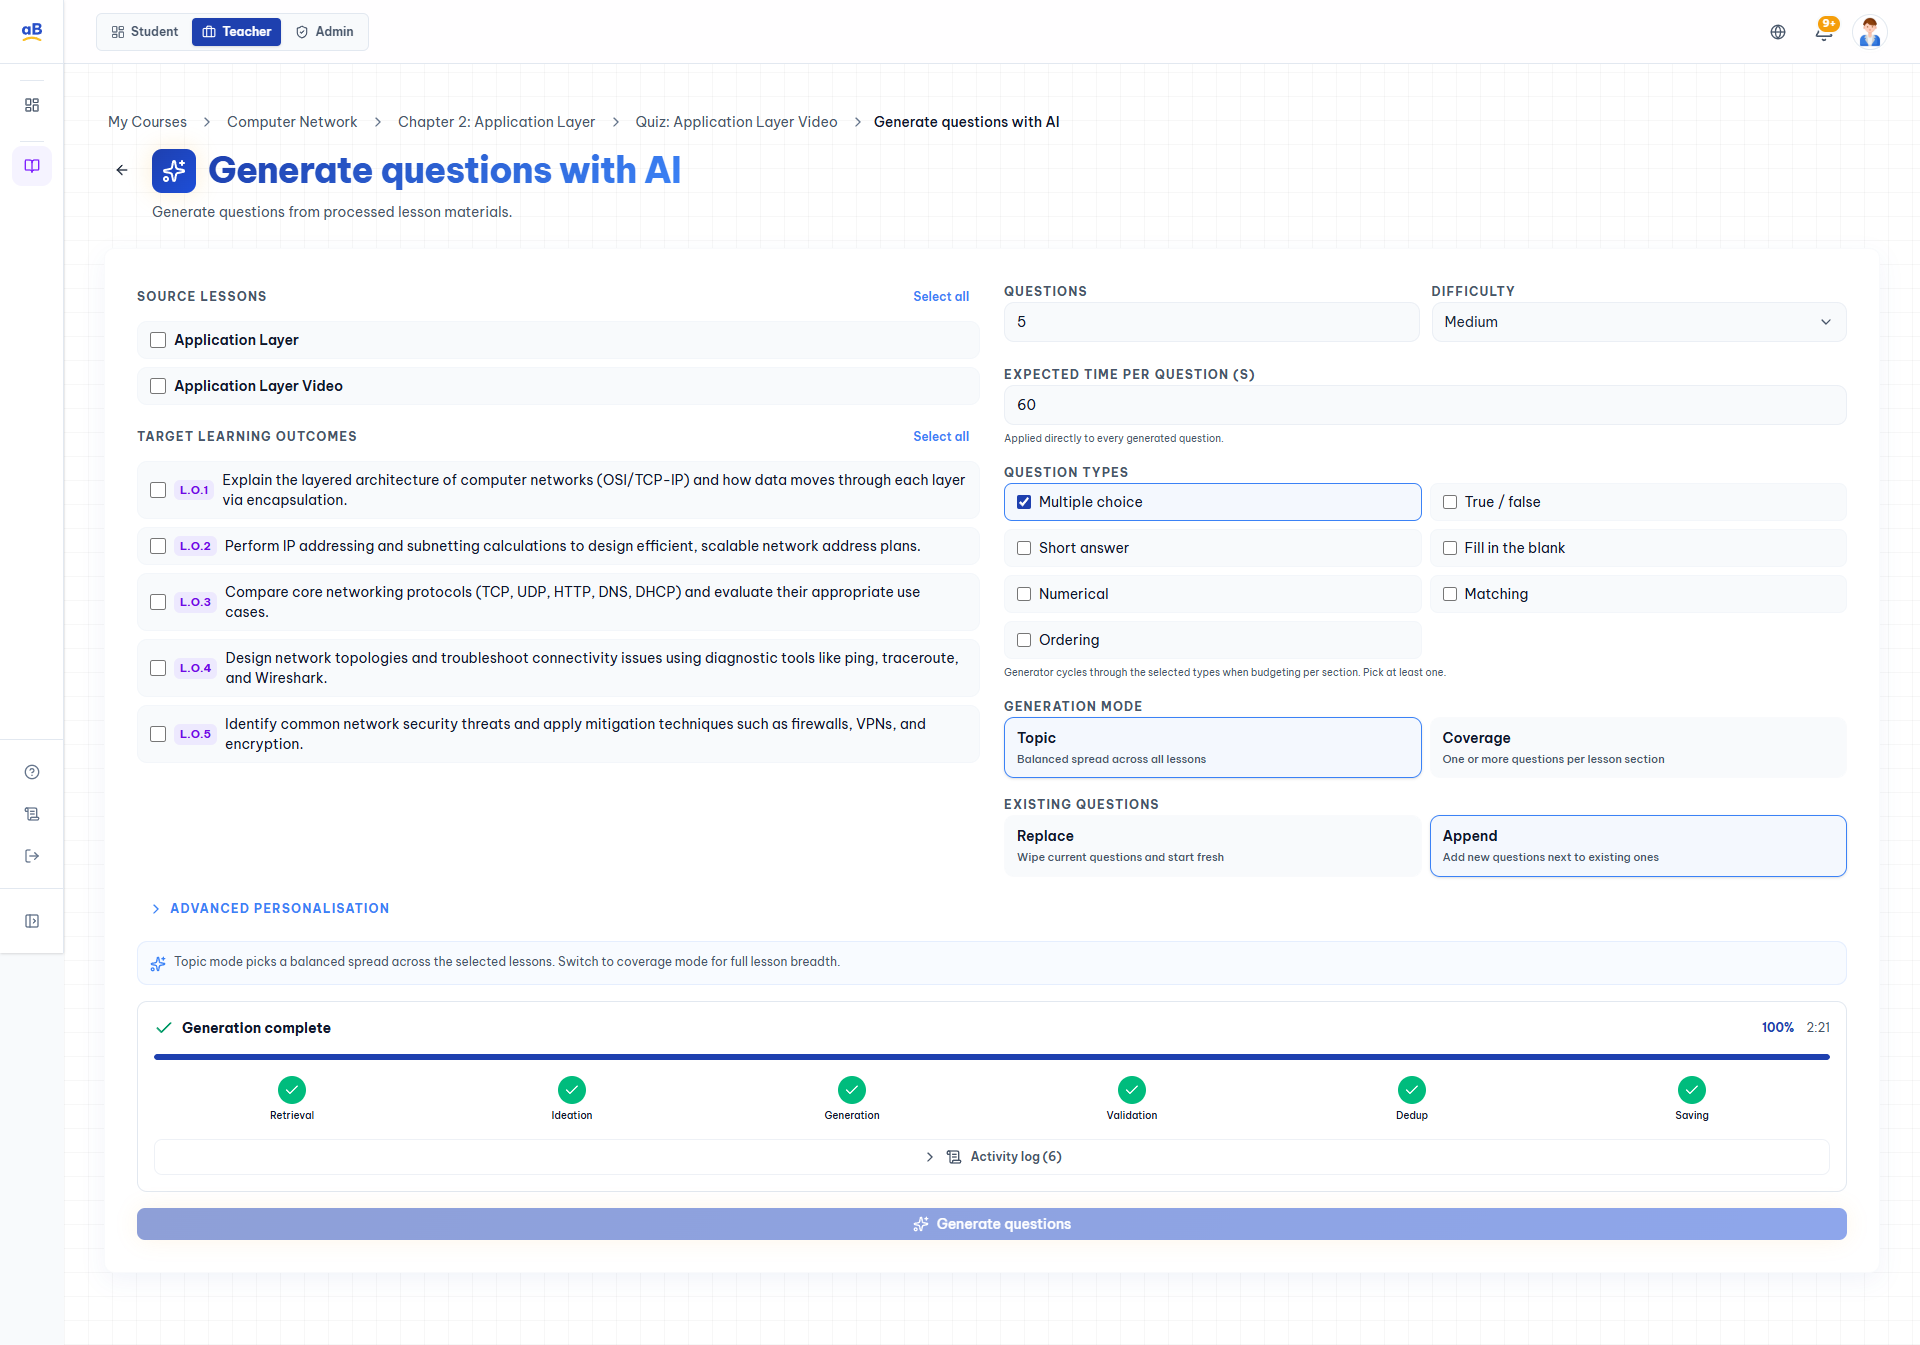
\includegraphics[width=0.85\textwidth]{graphics/screenshots/instructor_quiz_ai_modal.png}
  \caption{AI Quiz Generation modal --- Source-lesson selection, question count, mode and append/replace controls.}
  \label{fig:instructor_quiz_ai}
\end{figure}

The \textbf{Open generator} button on the quiz editor opens a modal that drives the AI quiz pipeline. The instructor selects one or more source lessons (only lessons whose materials have been processed are eligible), the desired number of questions, the difficulty band, and the question types (Multiple choice, True/False, Short answer, Fill in the blank). A generation-mode selector trades off two strategies: \textit{Topic} produces a balanced spread across all selected lessons, while \textit{Coverage} guarantees at least one question per section. An existing-questions selector decides between \textit{Replace} (wipe and regenerate) and \textit{Append} (add to the current bank). An advanced personalisation block, collapsed by default, exposes per-attempt prompt controls. Generated questions land in the editor in a \textit{Pending Review} state and only become visible to students after explicit instructor approval.

% ── Manager ─────────────────────────────────────────────────
\paragraph{Manager Dashboard}

\begin{figure}[H]
  \centering
  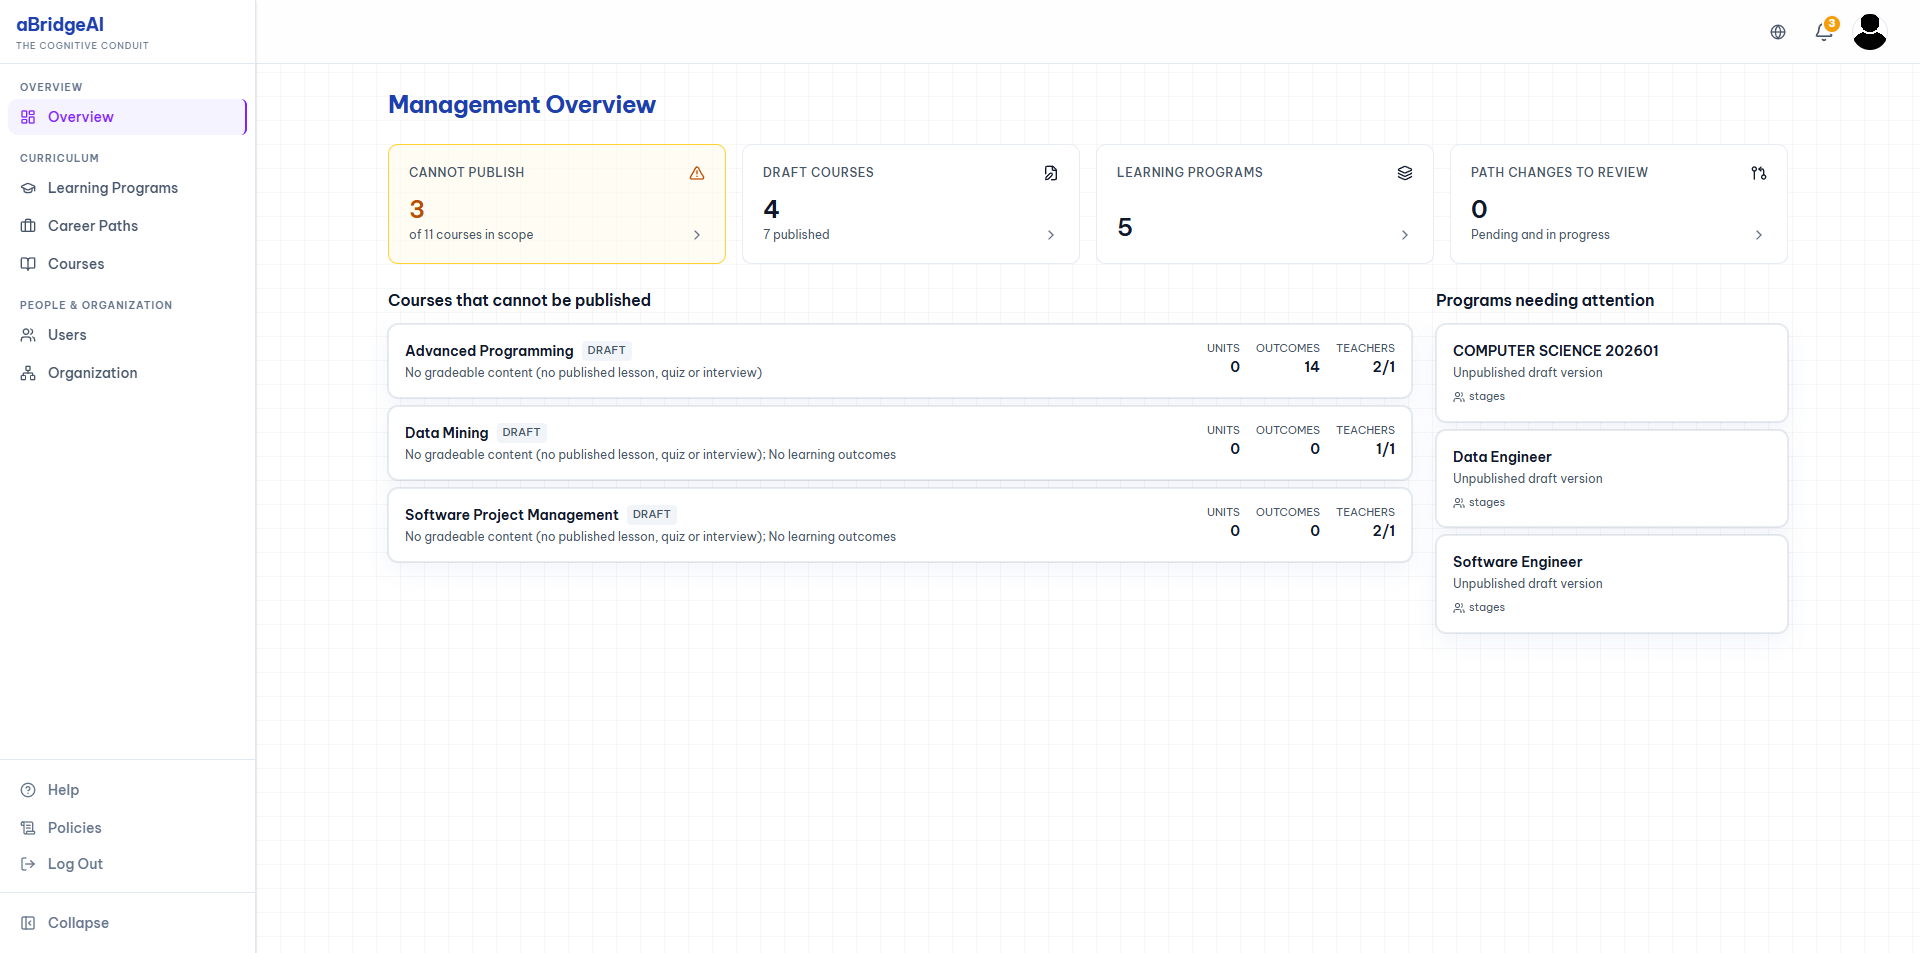
\includegraphics[width=\textwidth]{graphics/screenshots/manager_dashboard.png}
  \caption{Manager Dashboard --- Management overview with curriculum health stats, unpublishable courses, and programs needing attention.}
  \label{fig:manager_dashboard}
\end{figure}

The manager dashboard (\path|/manager|) is the operational hub for curriculum coordinators. Four stat cards summarise the health of the course catalogue --- Cannot Publish (courses lacking gradeable content), Draft Courses, Learning Programs, and Path Changes to Review. Below the cards, the left column lists courses that cannot be published with their blocking reasons (e.g.\ ``No gradeable content (no published lesson, quiz or interview)'', ``No learning outcomes''), unit count, outcome count, and assigned teachers. The right column surfaces learning programs and career paths that need attention, flagging unpublished draft versions and pending stage configurations. The layout prioritises actionable items so that managers can triage curriculum quality without navigating into individual course or path editors.

% ── Administrator ───────────────────────────────────────────
\paragraph{Processing Queue}

\begin{figure}[H]
  \centering
  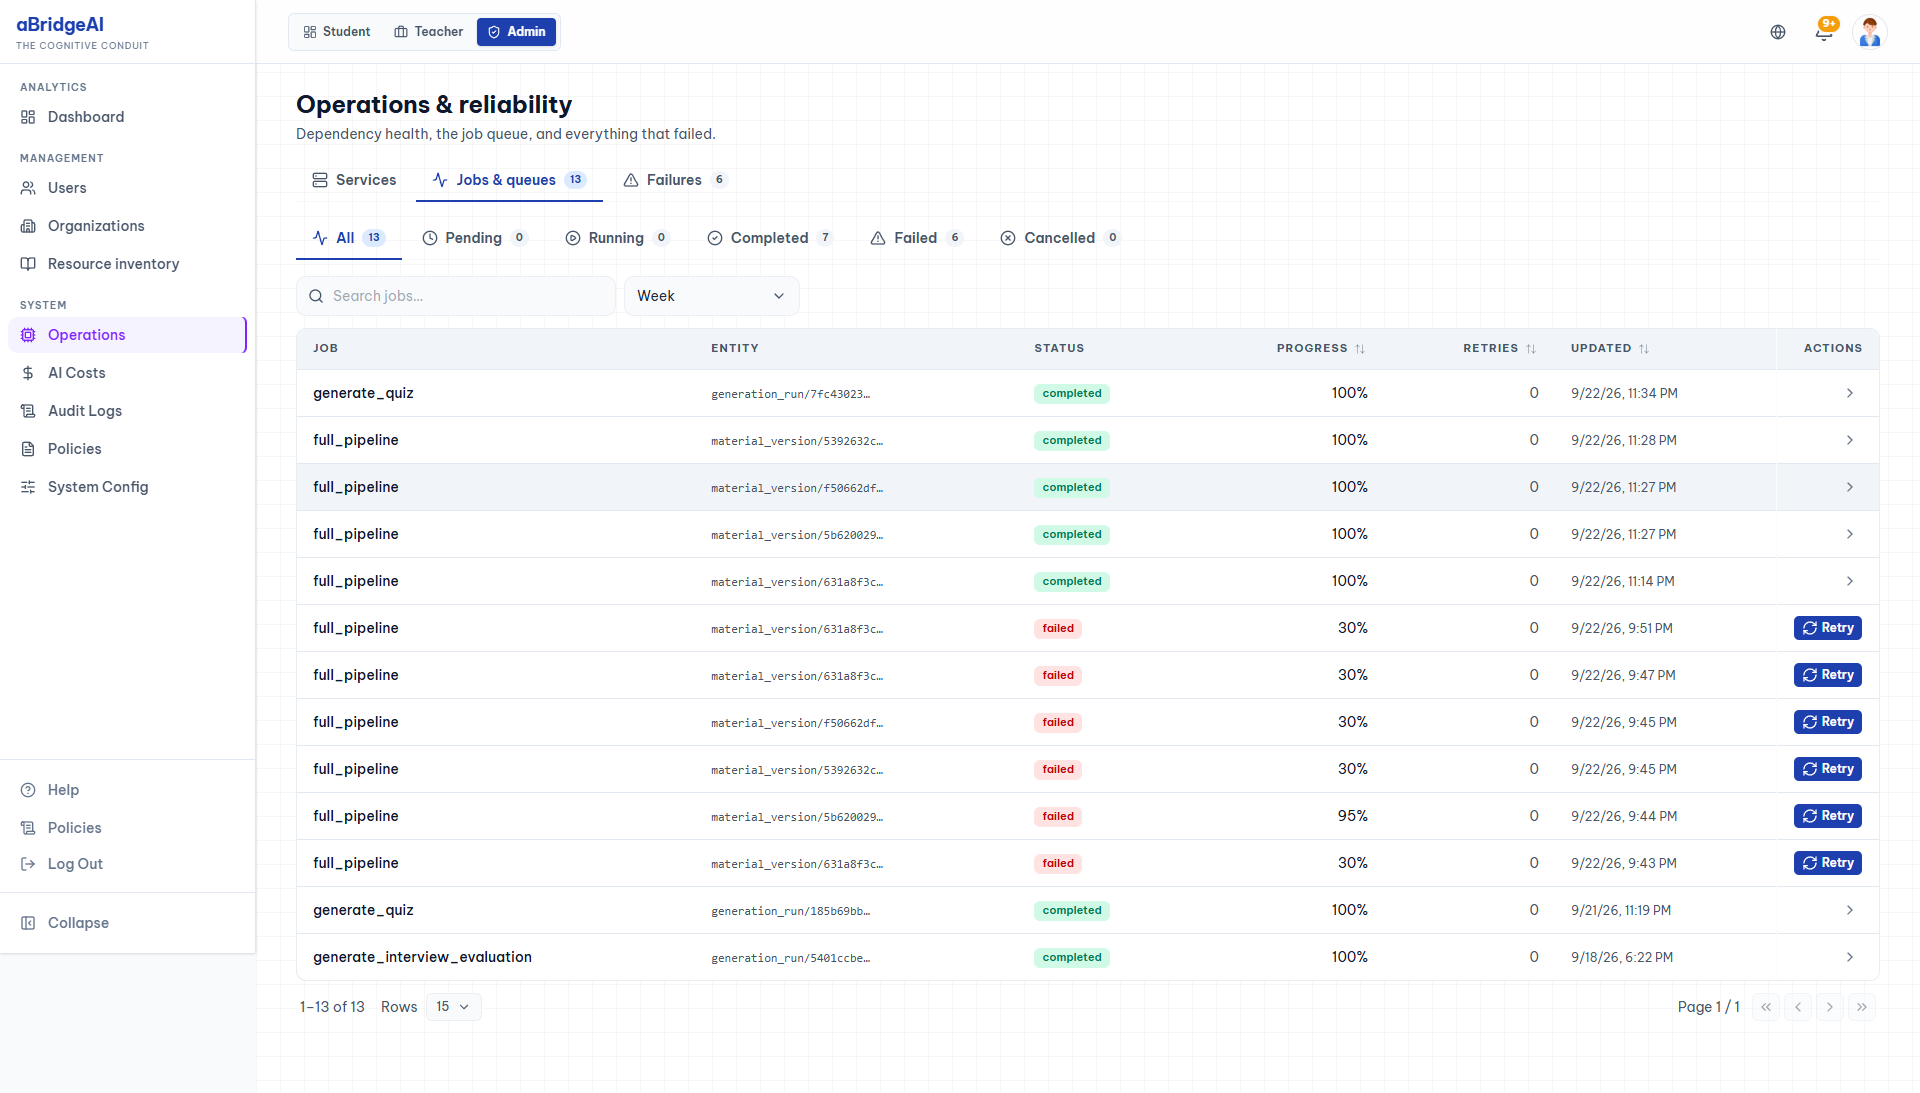
\includegraphics[width=\textwidth]{graphics/screenshots/admin_processing.png}
  \caption{Admin Processing Queue --- Background-job visibility with retry actions for failed runs.}
  \label{fig:admin_processing}
\end{figure}

The processing queue (\path|/admin/processing|) gives platform administrators direct visibility into the AI background-job pipeline (material ingestion, embedding, quiz generation, validation). Stat cards report the current backlog (Total, Pending, Running, Completed, Failed, Cancelled). A status-pill filter (\textit{All}, \textit{Pending}, \textit{Running}, \textit{Completed}, \textit{Failed}, \textit{Cancelled}) narrows the table, which lists the job type (\path|generate_quiz|, \path|full_pipeline|, \dots), the target entity ID, status, progress, retry count, last update, and a per-row \textbf{Retry} action for failed jobs. This is the operations console for the worker tier; it complements the per-course \textit{AI Material Hub} indicator visible to instructors.

\paragraph{AI Costs}

\begin{figure}[H]
  \centering
  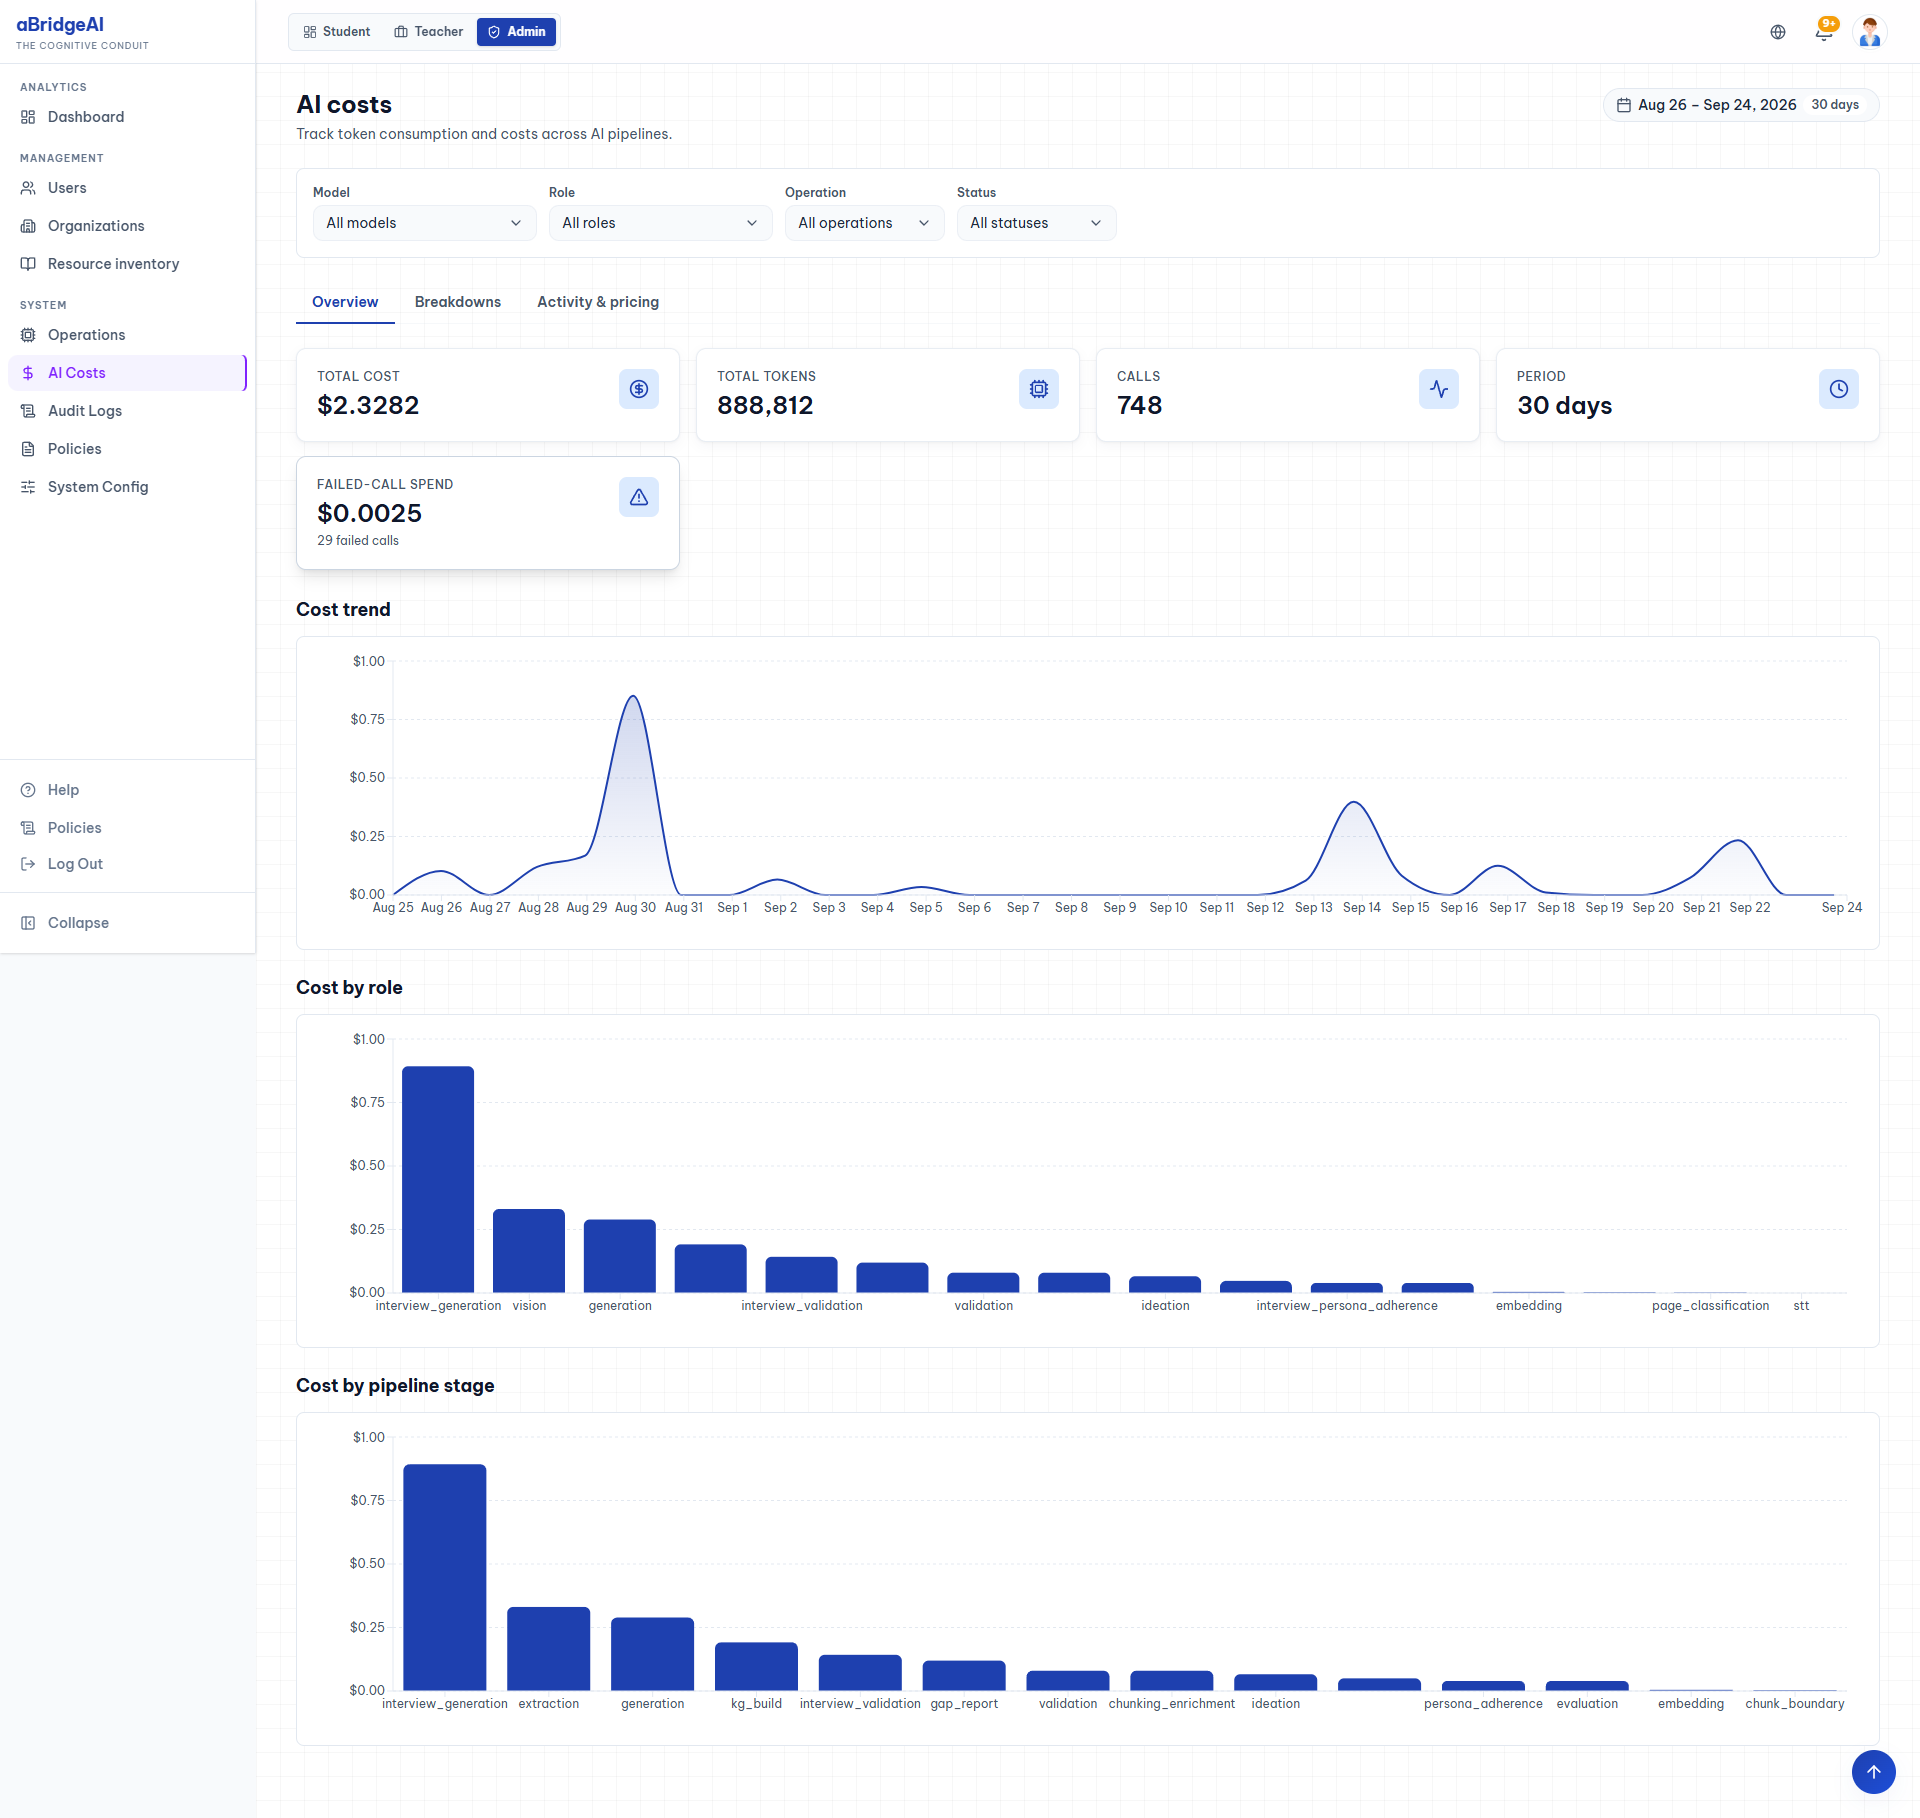
\includegraphics[width=\textwidth]{graphics/screenshots/admin_ai_costs.png}
  \caption{Admin AI Costs --- Token consumption and spend across pipeline roles and stages.}
  \label{fig:admin_ai_costs}
\end{figure}

The AI Costs page (\path|/admin/ai-costs|) exposes platform-wide spend on language-model and embedding APIs. A time-range selector (Last 24 hours, Last 7 days, Last 30 days) refilters every metric on the page. Summary cards report Total Cost, Total Tokens, total API Calls, and the active period. Two bar charts break the spend down by \textit{role} (embedding, ideation, chunking enrichment, generation, validation) and by \textit{pipeline stage}. The chart series reuse the platform palette (academic blue + amber) so administrators can correlate cost with backlog health on the Processing page without a context switch.

% ────────────────────────────────────────────────────────────
\subsubsection{Navigation Architecture}
% ────────────────────────────────────────────────────────────

\begin{longtable}{|p{0.22\textwidth}|p{0.20\textwidth}|p{0.46\textwidth}|}
  \caption{Navigation Components by Context} \label{tab:nav_components} \\
  \hline
  \textbf{Component} & \textbf{Context} & \textbf{Function} \\
  \hline
  \endfirsthead
  \multicolumn{3}{c}{\small\tablename~\thetable{} \textit{(continued)}} \\
  \hline
  \textbf{Component} & \textbf{Context} & \textbf{Function} \\
  \hline
  \endhead
  \hline
  \endfoot
  \path|TopNavBar| & Landing page only & Horizontal marketing nav: Explore, Login, Sign Up. Distinct from the authenticated shell. \\
  \hline
  \path|SideNavBar| & Authenticated (all) & Always rendered. Collapses to \path|w-16| (icons only) below the \path|md| breakpoint or by user toggle; expands to \path|w-64| with full labels. Receives a role-specific \path|navItems| array as a prop. \\
  \hline
  \path|ContentTopBar| & Authenticated (all) & Sticky page header carrying the current page title, language selector (i18n), notification bell, and user avatar with menu. \\
  \hline
  \path|AppShell| & Authenticated (all) & Orchestrates \path|SideNavBar| + \path|ContentTopBar| + main content into a responsive layout. Receives a \path|navItems| array, making it fully reusable across student, teacher, and admin route groups with no per-role layout code. \\
  \hline
  \path|Footer| & Landing page only & Marketing footer with product links and legal copy. \\
  \hline
\end{longtable}

The \path|AppShell| component is the structural keystone of the authenticated experience. The shell itself is role-agnostic; role differentiation is communicated through the \path|navItems| prop (defined in \path|src/lib/navigation.ts|) and through the active accent colour on the sidebar. Below the \path|md| breakpoint the sidebar overlays the page content via a backdrop rather than pushing it, keeping the main column readable on narrow screens.

% ────────────────────────────────────────────────────────────
\subsubsection{Design System Summary}
% ────────────────────────────────────────────────────────────

\begin{longtable}{|p{0.22\textwidth}|p{0.30\textwidth}|p{0.36\textwidth}|}
  \caption{Design System Tokens} \label{tab:design_tokens} \\
  \hline
  \textbf{Token Category} & \textbf{Value} & \textbf{Usage} \\
  \hline
  \endfirsthead
  \multicolumn{3}{c}{\small\tablename~\thetable{} \textit{(continued)}} \\
  \hline
  \textbf{Token Category} & \textbf{Value} & \textbf{Usage} \\
  \hline
  \endhead
  \hline
  \endfoot
  Page background & \path|#f8fafc| (slate-50) & Page surface in light mode. \\
  \hline
  Surface / Card & \path|#ffffff| & Cards, panels, dialogs. \\
  \hline
  Primary accent & \path|#1e40af| (blue-800) & Primary actions, active nav, links, chart series 1. \\
  \hline
  Secondary accent & \path|#3b82f6| (blue-500) & Secondary buttons, focus rings, chart series 2. \\
  \hline
  CTA / accent & \path|#f59e0b| (amber-500) & High-attention CTAs, AI affordances. \\
  \hline
  Success & \path|#16a34a| (green-600) & Published / completed state. \\
  \hline
  Warning & \path|#ea580c| (orange-600) & Drafts, pending review. \\
  \hline
  Danger & \path|#dc2626| (red-600) & Failed jobs, destructive actions. \\
  \hline
  Border & \path|#e2e8f0| (slate-200) & 1\,px borders on cards, inputs, tables. \\
  \hline
  Typography & Be Vietnam Pro (system-ui fallback) & All body and UI text; full Vietnamese diacritic support. \\
  \hline
  Component library & shadcn/ui + Radix UI & Dialogs, dropdowns, sheets, tooltips. \\
  \hline
  Icons & Lucide React & Single iconography source across the platform. \\
  \hline
  Charts & Recharts & Bar, line, area; reuses palette for chart series 1--5. \\
  \hline
  i18n keys & \path|src/lib/navigation.ts| + \path|src/locales/<lang>.json| & Translatable nav labels and copy. \\
  \hline
  Max modal depth & 1 stacked modal & Prevents nested-modal anti-patterns. \\
  \hline
  Base spacing unit & 4\,px & All spacing is a multiple of 4\,px. \\
  \hline
  Border radius (card) & 8\,px (\path|rounded-lg|) & Consistent card rounding; 10\,px hard cap project-wide. \\
  \hline
  Sidebar widths & 64\,px collapsed / 256\,px expanded & \path|w-16| / \path|w-64|; collapse driven by viewport width and user toggle. \\
  \hline
\end{longtable}

\clearpage
\section{Test Case Specifications}
\label{appendix:testcases}

% Specification tables are reference material, not prose: a step down in
% size and a tighter row stretch cost nothing in legibility and a great
% deal in printed bulk. The stretch is set here as well as on the
% individual tables, because not every table in this appendix declares one.
% Grouped so neither change leaks into the appendix that follows.
\begingroup
\small
\renewcommand{\arraystretch}{1.12}


% ============================ Module 1: Authentication & Access Control ====================
\paragraph{Authentication and Access Control}

\renewcommand{\arraystretch}{1.12}
\begin{longtable}{|>{\centering\arraybackslash}m{0.06\textwidth}|>{\centering\arraybackslash}m{0.08\textwidth}|>{\centering\arraybackslash}m{0.10\textwidth}|m{0.20\textwidth}|m{0.22\textwidth}|m{0.23\textwidth}|}
\caption{Test Cases: Authentication \& Access Control}
\label{tab:tc_auth_access} \\
\hline
\textbf{ID} &
\multicolumn{1}{>{\centering\arraybackslash}m{0.08\textwidth}|}{\textbf{Req}} &
\multicolumn{1}{>{\centering\arraybackslash}m{0.10\textwidth}|}{\textbf{Level}} &
\multicolumn{1}{>{\centering\arraybackslash}m{0.20\textwidth}|}{\textbf{Input}} &
\multicolumn{1}{>{\centering\arraybackslash}m{0.22\textwidth}|}{\textbf{Expected Result}} &
\multicolumn{1}{>{\centering\arraybackslash}m{0.23\textwidth}|}{\textbf{Exception}} \\
\hline
\endfirsthead

\multicolumn{6}{c}%
{{\bfseries Table \thetable\ -- Continued from previous page}} \\
\hline
\textbf{ID} &
\multicolumn{1}{>{\centering\arraybackslash}m{0.08\textwidth}|}{\textbf{Req}} &
\multicolumn{1}{>{\centering\arraybackslash}m{0.10\textwidth}|}{\textbf{Level}} &
\multicolumn{1}{>{\centering\arraybackslash}m{0.20\textwidth}|}{\textbf{Input}} &
\multicolumn{1}{>{\centering\arraybackslash}m{0.22\textwidth}|}{\textbf{Expected Result}} &
\multicolumn{1}{>{\centering\arraybackslash}m{0.23\textwidth}|}{\textbf{Exception}} \\
\hline
\endhead

\hline \multicolumn{6}{|r|}{{Continued on next page}} \\ \hline
\endfoot

\hline
\endlastfoot

% --- FR-1.1: Google SSO and Logout ---
TC-1.1.1 & FR-1.1 & System & User initiates login using Google SSO & System redirects the user to Google OAuth and authenticates the user after a successful callback & Login fails if the OAuth callback is invalid or the Google account is not authorised \\ \hline
TC-1.1.2 & FR-1.1 & System & Authenticated user clicks logout & User is logged out and redirected to the login page & Logout remains idempotent if the session has already expired \\ \hline

% --- FR-1.2: Session Management ---
TC-1.2.1 & FR-1.2 & System & User completes Google SSO successfully & System creates an authenticated session and issues valid access and refresh tokens & Session is not created if user identity cannot be mapped or provisioned \\ \hline
TC-1.2.2 & FR-1.2 & Integration & User sends a request with an expired access token and valid refresh token & System refreshes the session and rotates the refresh token & Refresh is rejected if the refresh token is expired, revoked, or reused \\ \hline
TC-1.2.3 & FR-1.2 & System & IT administrator disables an active user account & All active sessions for that account are revoked and protected resources become inaccessible & Historical user data remains preserved after account disablement \\ \hline

% --- FR-1.3: Two-Factor Authentication ---
TC-1.3.1 & FR-1.3 & System & User with MFA enabled logs in and enters a valid authenticator-app code & MFA verification succeeds and the user can access protected features & Invalid or expired verification codes are rejected \\ \hline
TC-1.3.2 & FR-1.3 & System & User enters a valid one-time recovery code & Recovery code is accepted and marked as used & Used recovery codes cannot be reused \\ \hline

% --- FR-1.4: Recent Second-Factor Verification ---
TC-1.4.1 & FR-1.4 & System & User attempts to regenerate recovery codes after recent MFA verification & Operation is allowed and new recovery codes are generated & Operation is blocked if MFA verification is outside the freshness window \\ \hline
TC-1.4.2 & FR-1.4 & System & User attempts to disable MFA without recent second-factor verification & System requires re-verification before allowing the operation & MFA cannot be disabled through direct API bypass \\ \hline

% --- FR-1.5: Role and Permission-Based Access Control ---
TC-1.5.1 & FR-1.5 & System & User accesses a protected backend route with sufficient permission & Request is allowed and the protected resource is returned & Request is denied if the user lacks the required permission \\ \hline
TC-1.5.2 & FR-1.5 & System & Frontend renders actions for a user with limited permissions & UI hides or disables actions outside the user's effective permissions & Hidden actions remain protected server-side if called directly \\ \hline

% --- FR-1.6: Authentication and Access Audit Events ---
TC-1.6.1 & FR-1.6 & System & User performs login, logout, and MFA verification actions & System records corresponding auditable events & Audit logging failure does not expose sensitive authentication data \\ \hline
TC-1.6.2 & FR-1.6 & System & Administrator changes account-security or access-control settings & System records actor, action, target, and timestamp in the audit log & Audit records cannot be modified by non-authorised users \\ \hline

\end{longtable}


% ============================ Module 2: Organization & User Management ====================
\paragraph{Organization and User Management}

\renewcommand{\arraystretch}{1.12}
\begin{longtable}{|>{\centering\arraybackslash}m{0.06\textwidth}|>{\centering\arraybackslash}m{0.08\textwidth}|>{\centering\arraybackslash}m{0.10\textwidth}|m{0.20\textwidth}|m{0.22\textwidth}|m{0.23\textwidth}|}
\caption{Test Cases: Organization \& User Management}
\label{tab:tc_org} \\
\hline
\textbf{ID} &
\multicolumn{1}{>{\centering\arraybackslash}m{0.08\textwidth}|}{\textbf{Req}} &
\multicolumn{1}{>{\centering\arraybackslash}m{0.10\textwidth}|}{\textbf{Level}} &
\multicolumn{1}{>{\centering\arraybackslash}m{0.20\textwidth}|}{\textbf{Input}} &
\multicolumn{1}{>{\centering\arraybackslash}m{0.22\textwidth}|}{\textbf{Expected Result}} &
\multicolumn{1}{>{\centering\arraybackslash}m{0.23\textwidth}|}{\textbf{Exception}} \\
\hline
\endfirsthead

\multicolumn{6}{c}%
{{\bfseries Table \thetable\ -- Continued from previous page}} \\
\hline
\textbf{ID} &
\multicolumn{1}{>{\centering\arraybackslash}m{0.08\textwidth}|}{\textbf{Req}} &
\multicolumn{1}{>{\centering\arraybackslash}m{0.10\textwidth}|}{\textbf{Level}} &
\multicolumn{1}{>{\centering\arraybackslash}m{0.20\textwidth}|}{\textbf{Input}} &
\multicolumn{1}{>{\centering\arraybackslash}m{0.22\textwidth}|}{\textbf{Expected Result}} &
\multicolumn{1}{>{\centering\arraybackslash}m{0.23\textwidth}|}{\textbf{Exception}} \\
\hline
\endhead

\hline \multicolumn{6}{|r|}{{Continued on next page}} \\ \hline
\endfoot

\hline
\endlastfoot

% --- FR-2.1: Tenant Provisioning ---
TC-2.1.1 & FR-2.1 & System & IT administrator provisions a new tenant organisation with required details and an initial Educational Manager & Organisation is created and the selected user receives the initial manager role & Provisioning fails if required organisation information is missing or invalid \\ \hline

% --- FR-2.2: Organisation Lifecycle Management ---
TC-2.2.1 & FR-2.2 & System & IT administrator updates an existing organisation's basic information & Updated information is saved and reflected in organisation views & Duplicate or invalid organisation metadata is rejected \\ \hline
TC-2.2.2 & FR-2.2 & System & IT administrator changes an organisation status to inactive, archived, or soft-deleted & Organisation lifecycle state is updated and access rules follow the new state & Invalid lifecycle transitions are rejected \\ \hline

% --- FR-2.3: Bulk Student Enrollment ---
TC-2.3.1 & FR-2.3 & System & Educational Manager uploads a CSV containing valid and invalid student rows & Valid student accounts are created or enrolled, and invalid rows are reported without aborting the whole batch & Duplicate or malformed email rows are listed in the validation report \\ \hline

% --- FR-2.4: Career Pathways ---
TC-2.4.1 & FR-2.4 & System & Educational Manager creates a career pathway with an ordered sequence of courses & Career pathway is saved and course order is preserved & Pathway creation is rejected if required course references are invalid \\ \hline
TC-2.4.2 & FR-2.4 & System & Educational Manager reorders courses within a pathway & New order is saved and reflected in pathway views & Reordering fails if the manager does not belong to the organisation \\ \hline

% --- FR-2.5: Teacher Assignment ---
TC-2.5.1 & FR-2.5 & System & Educational Manager assigns a Teacher to a course within their organisation & Teacher is linked to the course and can access authoring features & Assignment fails if the teacher is inactive or outside the organisation \\ \hline

% --- FR-2.6: Tenant-Scoped Manager Access ---
TC-2.6.1 & FR-2.6 & System & Educational Manager queries users, courses, or reports from their own organisation & System returns only data within the manager's tenant organisation & Cross-tenant records are not returned \\ \hline
TC-2.6.2 & FR-2.6 & System & Educational Manager attempts to access another tenant's data via direct URL or API call & Access is denied & No partial cross-tenant data is leaked \\ \hline

% --- FR-2.7: Organisation and Org Unit Association ---
TC-2.7.1 & FR-2.7 & Integration & New account is provisioned using an email domain registered to an organisation & Account is automatically associated with the matching organisation & Account remains unassigned or requires manual review if no matching domain exists \\ \hline

% --- FR-2.8: User Profile Management ---
TC-2.8.1 & FR-2.8 & System & Authenticated user updates display name, avatar, bio, or external links & Profile changes are saved and reflected in the user's account page & Invalid external link formats are rejected \\ \hline

% --- FR-2.9: Organisation Domain Management ---
TC-2.9.1 & FR-2.9 & System & IT administrator adds, removes, or toggles auto-provisioning for an organisation email domain & Domain settings are updated and used for future account provisioning & Duplicate domain registration is rejected \\ \hline

% --- FR-2.10: Organisation Membership Records ---
TC-2.10.1 & FR-2.10 & System & Authorised manager updates a user's organisation membership and identifier code & Membership record is saved and visible in organisation membership views & Update is denied if the manager lacks organisation-management permission \\ \hline

% --- FR-2.11: Enable or Disable User Accounts ---
TC-2.11.1 & FR-2.11 & System & IT administrator disables a user account across tenant organisations & Disabled user can no longer access protected system resources & User records and historical activity remain preserved \\ \hline

% --- FR-2.12: Faculty Structure Management ---
TC-2.12.1 & FR-2.12 & System & Authorised administrator creates a faculty, renames it, then archives it together with its subordinate units & Faculty is created, renamed and archived with its subordinate units, and the organisation's units are viewable both as a flat list and as a nested tree carrying descendant counts & Archiving is refused when the caller lacks organisation-unit management permission \\ \hline

% --- FR-2.13: Faculty Staff Affiliation ---
TC-2.13.1 & FR-2.13 & System & Faculty Dean grants faculty staff affiliation to several users in one bulk operation, then revokes one & All selected users become active staff of the faculty in a single operation, and the revoked user is no longer active staff; affiliation alone grants no additional role & The operation is rejected when any selected user belongs to another organisation \\ \hline

% --- FR-2.13: Faculty Staffing Gates Course Staffing ---
TC-2.13.2 & FR-2.13 & System & Manager assigns a teacher to a course whose owning faculty the teacher is not active staff of & Assignment is refused and the course's teacher list is unchanged & System reports that the teacher is not staff of the course's faculty \\ \hline

% --- FR-2.14: Course Invitation Codes ---
TC-2.14.1 & FR-2.14 & System & Educational Manager issues a course invitation code with a maximum use count and an expiry date, amends it, then revokes it & Code is issued with the configured limits, the amendment takes effect for subsequent uses, and the revoked code stops working while its record is retained for audit & Redemption is refused once the code is expired, exhausted or revoked \\ \hline

% --- FR-2.15: Course Enrolment Lifecycle ---
TC-2.15.1 & FR-2.15 & System & Manager unenrols an active student from a course, then re-enrols the same student & Unenrolment is recorded as a dropped enrolment rather than deleted, and the re-enrolment reactivates the existing record with its origin preserved & A duplicate enrolment row is never created for a student already recorded on the course \\ \hline

\end{longtable}


% ============================ Module 3: Course & Material Management ====================
\paragraph{Course and Material Management}

\renewcommand{\arraystretch}{1.12}
\begin{longtable}{|>{\centering\arraybackslash}m{0.06\textwidth}|>{\centering\arraybackslash}m{0.08\textwidth}|>{\centering\arraybackslash}m{0.10\textwidth}|m{0.20\textwidth}|m{0.22\textwidth}|m{0.23\textwidth}|}
\caption{Test Cases: Course \& Material Management}
\label{tab:tc_course_material} \\
\hline
\textbf{ID} &
\multicolumn{1}{>{\centering\arraybackslash}m{0.08\textwidth}|}{\textbf{Req}} &
\multicolumn{1}{>{\centering\arraybackslash}m{0.10\textwidth}|}{\textbf{Level}} &
\multicolumn{1}{>{\centering\arraybackslash}m{0.20\textwidth}|}{\textbf{Input}} &
\multicolumn{1}{>{\centering\arraybackslash}m{0.22\textwidth}|}{\textbf{Expected Result}} &
\multicolumn{1}{>{\centering\arraybackslash}m{0.23\textwidth}|}{\textbf{Exception}} \\
\hline
\endfirsthead

\multicolumn{6}{c}%
{{\bfseries Table \thetable\ -- Continued from previous page}} \\
\hline
\textbf{ID} &
\multicolumn{1}{>{\centering\arraybackslash}m{0.08\textwidth}|}{\textbf{Req}} &
\multicolumn{1}{>{\centering\arraybackslash}m{0.10\textwidth}|}{\textbf{Level}} &
\multicolumn{1}{>{\centering\arraybackslash}m{0.20\textwidth}|}{\textbf{Input}} &
\multicolumn{1}{>{\centering\arraybackslash}m{0.22\textwidth}|}{\textbf{Expected Result}} &
\multicolumn{1}{>{\centering\arraybackslash}m{0.23\textwidth}|}{\textbf{Exception}} \\
\hline
\endhead

\hline \multicolumn{6}{|r|}{{Continued on next page}} \\ \hline
\endfoot

\hline
\endlastfoot

% --- FR-3.1: Course Lifecycle ---
TC-3.1.1 & FR-3.1 & System & Teacher creates a course in draft state with required metadata & Course is saved as draft and is not visible to students until published & Course creation fails if required metadata is missing \\ \hline
TC-3.1.2 & FR-3.1 & System & Authorised user archives or restores a soft-deleted course & Course lifecycle state is updated correctly & Restore fails if the user lacks administrative permission \\ \hline

% --- FR-3.2: Course Structure and Unlock Rules ---
TC-3.2.1 & FR-3.2 & System & Teacher creates ordered modules and learning items with prerequisites & Structure is saved and displayed in the configured order & Circular or invalid prerequisite rules are rejected \\ \hline

% --- FR-3.3: Material Upload and Processing ---
TC-3.3.1 & FR-3.3 & System & Teacher uploads a supported learning material using a standard or resumable upload flow & Material is stored, linked to the lesson, and queued for processing & Unsupported formats or failed uploads are rejected with an error message \\ \hline
TC-3.3.2 & FR-3.3 & System & Teacher re-runs processing for an existing material & Processing pipeline is restarted and new processed artefacts are generated & Re-run is blocked if the material is missing or inaccessible \\ \hline

% --- FR-3.4: Material Version History ---
TC-3.4.1 & FR-3.4 & System & Teacher uploads a replacement version of an existing material & New version becomes current while prior versions remain available for rollback or re-processing & Invalid replacement files do not overwrite the current version \\ \hline

% --- FR-3.5: Ingestion Progress ---
TC-3.5.1 & FR-3.5 & System & Teacher views ingestion status for a material version & System displays processing status, percent completion, and failure reason if applicable & Failed processing jobs show actionable error information \\ \hline

% --- FR-3.6: Material Visibility ---
TC-3.6.1 & FR-3.6 & System & Teacher marks a material as hidden while the course remains published & Students cannot access the hidden material & Teachers can still view hidden material in authoring mode \\ \hline

% --- FR-3.7: Student Course and Material Access ---
TC-3.7.1 & FR-3.7 & System & Enrolled student browses published courses and opens approved material & Student can view course details and stream or download approved material via a presigned URL & Unpublished or invisible materials are not accessible \\ \hline

% --- FR-3.8: Administrative Course Inspection ---
TC-3.8.1 & FR-3.8 & System & IT administrator opens course processing history and aggregate statistics & System displays processing jobs, status history, and aggregate course statistics & Access is denied to users without administrative permission \\ \hline

% --- FR-3.9: Course Staffing with Multiple Titles ---
TC-3.9.1 & FR-3.9 & System & Authorised manager assigns two Course Instructors and one Teaching Assistant, grants a single teacher both titles, then re-assigns an already active teacher & Course carries multiple instructors and assistants, the dual-title teacher holds both on one assignment, the redundant re-assignment is treated as no change, and each newly assigned teacher is notified & Revoking an assignment expires it rather than deleting it, so the history remains \\ \hline

% --- FR-3.10: Pre-publication Readiness Checklist ---
TC-3.10.1 & FR-3.10 & System & Manager opens the readiness checklist for a course staffed below the configured minimum teacher count & Checklist reports staffing against the configured minimum and maximum, the number of gradeable curriculum units, and whether learning outcomes are present & Checklist is unavailable to a caller without course-management permission \\ \hline

% --- FR-3.11: Course Cloning at Selectable Depth ---
TC-3.11.1 & FR-3.11 & System & Authorised manager clones a published course selecting the shell together with the module skeleton and module prerequisites & A draft copy is created with a uniquely generated slug carrying the selected depth of content, and module prerequisites are preserved & Learner runtime data such as enrolments, attempts and grades is excluded from the copy \\ \hline

% --- FR-3.12: Lesson Knowledge Map ---
TC-3.12.1 & FR-3.12 & System & Teacher opens the knowledge map derived from a lesson's ingested materials, curates it, and publishes it & Concepts and relationships are derived from the lesson's materials, the curated map is saved, and Students see the map only after publication & An unpublished map is not exposed to Students \\ \hline

% --- FR-3.13: Material Preprocessing and Quarantine ---
TC-3.13.1 & FR-3.13 & System & Teacher selects a text-preprocessing mode for a material whose extraction yields units unsafe to index & Unsafe units are quarantined with the reason and the number of occurrences, the Teacher may restore or confirm each one, and a preview of the resulting content chunks is available & Quarantined units are never indexed until the Teacher resolves them \\ \hline

% --- FR-3.14: Ingestion Recovery ---
TC-3.14.1 & FR-3.14 & System & A processing job is left pending with no live background task and an upload is abandoned midway & The stranded job is reconciled, abandoned generation runs are finalised, and orphaned uploads are removed by the periodic sweep & Recovery never re-runs work that has already completed successfully \\ \hline

% --- FR-3.15: Lesson Discussion Topics ---
TC-3.15.1 & FR-3.15 & System & Course manager opens a discussion topic on a lesson, an enrolled Student comments, then the manager closes the topic & Topic is created and editable by the manager, the enrolled Student's comment is posted, and the closed topic accepts no further Student comments while managers may still post & A user who is not enrolled and cannot manage the course receives not-found rather than a permission error \\ \hline

\end{longtable}


% ============================ Module 4: Learning Loop & Adaptive Quiz ====================
\paragraph{Learning Loop and Adaptive Quiz}

\renewcommand{\arraystretch}{1.12}
\begin{longtable}{|>{\centering\arraybackslash}m{0.06\textwidth}|>{\centering\arraybackslash}m{0.08\textwidth}|>{\centering\arraybackslash}m{0.10\textwidth}|m{0.20\textwidth}|m{0.22\textwidth}|m{0.23\textwidth}|}
\caption{Test Cases: Learning Loop \& Adaptive Quiz}
\label{tab:tc_learning_loop} \\
\hline
\textbf{ID} &
\multicolumn{1}{>{\centering\arraybackslash}m{0.08\textwidth}|}{\textbf{Req}} &
\multicolumn{1}{>{\centering\arraybackslash}m{0.10\textwidth}|}{\textbf{Level}} &
\multicolumn{1}{>{\centering\arraybackslash}m{0.20\textwidth}|}{\textbf{Input}} &
\multicolumn{1}{>{\centering\arraybackslash}m{0.22\textwidth}|}{\textbf{Expected Result}} &
\multicolumn{1}{>{\centering\arraybackslash}m{0.23\textwidth}|}{\textbf{Exception}} \\
\hline
\endfirsthead

\multicolumn{6}{c}%
{{\bfseries Table \thetable\ -- Continued from previous page}} \\
\hline
\textbf{ID} &
\multicolumn{1}{>{\centering\arraybackslash}m{0.08\textwidth}|}{\textbf{Req}} &
\multicolumn{1}{>{\centering\arraybackslash}m{0.10\textwidth}|}{\textbf{Level}} &
\multicolumn{1}{>{\centering\arraybackslash}m{0.20\textwidth}|}{\textbf{Input}} &
\multicolumn{1}{>{\centering\arraybackslash}m{0.22\textwidth}|}{\textbf{Expected Result}} &
\multicolumn{1}{>{\centering\arraybackslash}m{0.23\textwidth}|}{\textbf{Exception}} \\
\hline
\endhead

\hline \multicolumn{6}{|r|}{{Continued on next page}} \\ \hline
\endfoot

\hline
\endlastfoot

% --- FR-4.1: Quiz Question Authoring and Review ---
TC-4.1.1 & FR-4.1 & Integ-ration & Teacher drafts quiz questions from ingested course content & Questions are generated from source content, retain source references, and enter review state & Questions without valid source references are flagged for review \\ \hline
TC-4.1.2 & FR-4.1 & System & Teacher edits, approves, rejects, or reuses quiz questions & Question state and revision history are updated correctly & Students cannot access unapproved questions, no question can be authored, imported, or generated unless the quiz is a draft, and a generation run that would replace existing questions is refused once a learner attempt or spaced-repetition card state exists \\ \hline

% --- FR-4.2: Quiz and SR Configuration ---
TC-4.2.1 & FR-4.2 & System & Teacher configures quiz settings and sets $T_{\text{exp}}$ for every live question & Quiz can be published and settings are applied to student attempts & Publication is blocked if any live question has no $T_{\text{exp}}$; on a published quiz only the title, description, schedule, and reminders remain editable, and an archived quiz refuses every edit \\ \hline

% --- FR-4.3: Student Quiz Session ---
TC-4.3.1 & FR-4.3 & System & Student submits a quiz answer with response time and optional hint usage & System records correctness, response time, and hint usage for the answer & Attempts are blocked when retake policy or cooldown rules are violated \\ \hline

% --- FR-4.4: Q Derivation and Hybrid SM-2 Update ---
TC-4.4.1 & FR-4.4 & Unit & System receives correctness, hint usage, $T_{\text{actual}}$, and $T_{\text{exp}}$ for a card response & System derives the correct $Q$ value using the configured mapping & Invalid or missing timing data is rejected or handled by a defined fallback \\ \hline
TC-4.4.2 & FR-4.4 & Integ-ration & Card response produces a derived $Q$ value & Student-card SM-2 state is updated with EF, interval, due date, calibration, and jitter rules & EF never falls below the configured floor \\ \hline

% --- FR-4.5: Lesson Access Gate ---
TC-4.5.1 & FR-4.5 & System & Student satisfies prerequisite completion and EF coverage threshold $\tau$ & Dependent lesson becomes accessible & Lesson remains locked if prerequisite or coverage threshold is not satisfied \\ \hline

% --- FR-4.6: SR and Remediation Notifications ---
TC-4.6.1 & FR-4.6 & Integ-ration & A student's card becomes due for review & System delivers an in-app spaced-repetition reminder & Notification is not delivered if the card has already been reviewed \\ \hline
TC-4.6.2 & FR-4.6 & Integ-ration & Student fails a card linked to source material & System sends remediation notification linking to relevant material when available & Notification omits material link if no reliable source reference exists \\ \hline

% --- FR-4.7: Teacher Learning Analytics ---
TC-4.7.1 & FR-4.7 & System & Teacher opens learning-loop analytics for a course & System displays cohort retention, difficult cards, at-risk students, and per-student SR details & Empty state is shown if no quiz activity exists \\ \hline

% --- FR-4.8: Student Learning Dashboard ---
TC-4.8.1 & FR-4.8 & System & Student opens personal learning dashboard & System displays due cards, retention estimate, progression readiness, and course-level progress & Dashboard handles courses with no due cards gracefully \\ \hline

% --- FR-4.9: Manual Grading Queue ---
TC-4.9.1 & FR-4.9 & System & Student submits an attempt containing a code answer and a short-answer response that fails exact-match grading & Both answers are routed into the per-quiz manual grading queue, the attempt score is withheld while any answer is unmarked, and the score and pass decision are recomputed once every answer carries a mark & The attempt cannot be reported as graded while an unmarked answer remains \\ \hline

% --- FR-4.10: Grade of Record ---
TC-4.10.1 & FR-4.10 & System & Student completes several attempts on a quiz whose grading method is highest attempt, and a Teacher then regrades one of them & A single grade of record is derived by the configured method, refreshed after the regrade, and shown in the Teacher's gradebook & Changing the grading method never rewrites the stored attempts themselves \\ \hline

% --- FR-4.11: Answer-key Correction ---
TC-4.11.1 & FR-4.11 & System & Teacher corrects an answer key and requests a dry run before committing & Dry run reports every changed answer and the number of affected attempts, and the correction is applied only on explicit commit, recomputing affected scores and recording the operation for audit & No score changes while the correction remains an uncommitted dry run \\ \hline

% --- FR-4.12: Assessment Accommodations ---
TC-4.12.1 & FR-4.12 & System & Teacher grants a per-student accommodation extending the time limit where a conflicting per-group accommodation already exists, and the Student then starts an attempt & Accommodations resolve by student-over-group-over-quiz precedence and the resolved policy governs the attempt's window, due date, time limit, attempt ceiling, retake permission and cooldown & An accommodation belonging to another quiz is never applied \\ \hline

% --- FR-4.13: Score-band Feedback ---
TC-4.13.1 & FR-4.13 & System & Teacher defines score bands mapping percentage ranges to feedback messages, and a Student reviews a completed attempt & The band matching the Student's score is shown on attempt review & Feedback is withheld whenever the score itself is not disclosed to the Student \\ \hline

% --- FR-4.14: Curated Question Bank ---
TC-4.14.1 & FR-4.14 & System & Teacher copies existing questions into the course question bank, edits an approved item, then imports from the bank into a quiz & Duplicates are skipped rather than rejected during the copy, editing an approved item demotes it to draft, and only approved items are admitted when importing into a quiz & An archived item is never offered for import \\ \hline

% --- FR-4.15: Question Interchange Import and Export ---
TC-4.15.1 & FR-4.15 & System & Teacher imports a Moodle GIFT file and a Moodle XML file, then bulk-approves the results and bulk-assigns an expected response time & Questions are imported from both formats as pending review, bulk approval and bulk expected-time assignment apply to the selection, and questions export back to both formats & A malformed interchange file is rejected with the offending entry identified \\ \hline

% --- FR-4.16: Quiz Integrity Signals ---
TC-4.16.1 & FR-4.16 & System & Student loses window focus, switches tab and exits full screen during an in-progress attempt & Each signal is recorded in the append-only integrity store without interrupting the attempt, the Student is informed that monitoring is active, and the Teacher sees the resulting timeline beside the assessment audit trail & Signals reported after the attempt has ended are refused \\ \hline

% --- FR-4.17: Quiz Item Analysis ---
TC-4.17.1 & FR-4.17 & System & Teacher opens item analysis for a quiz including one question answered identically by every student & Facility index and discrimination index are reported per question, with an explanation where discrimination cannot be computed, alongside per-student response reports & Reports download as structured data, comma-separated values or a spreadsheet without altering the underlying attempts \\ \hline

% --- FR-4.18: Overdue Attempt Handling ---
TC-4.18.1 & FR-4.18 & System & A timed attempt reaches its deadline without the Student submitting & The attempt is closed according to the quiz's overdue policy by grading the completed work, extending the deadline by the configured grace period, or abandoning the attempt without a grade & An attempt already submitted is never reopened or re-closed by the sweep \\ \hline

\end{longtable}


% ============================ Module 5: Application Loop & Mock Interview ====================
\paragraph{Application Loop and Mock Interview}

\renewcommand{\arraystretch}{1.12}
\begin{longtable}{|>{\centering\arraybackslash}m{0.06\textwidth}|>{\centering\arraybackslash}m{0.08\textwidth}|>{\centering\arraybackslash}m{0.10\textwidth}|m{0.20\textwidth}|m{0.22\textwidth}|m{0.23\textwidth}|}
\caption{Test Cases: Application Loop \& Mock Interview}
\label{tab:tc_interview} \\
\hline
\textbf{ID} &
\multicolumn{1}{>{\centering\arraybackslash}m{0.08\textwidth}|}{\textbf{Req}} &
\multicolumn{1}{>{\centering\arraybackslash}m{0.10\textwidth}|}{\textbf{Level}} &
\multicolumn{1}{>{\centering\arraybackslash}m{0.20\textwidth}|}{\textbf{Input}} &
\multicolumn{1}{>{\centering\arraybackslash}m{0.22\textwidth}|}{\textbf{Expected Result}} &
\multicolumn{1}{>{\centering\arraybackslash}m{0.23\textwidth}|}{\textbf{Exception}} \\
\hline
\endfirsthead

\multicolumn{6}{c}%
{{\bfseries Table \thetable\ -- Continued from previous page}} \\
\hline
\textbf{ID} &
\multicolumn{1}{>{\centering\arraybackslash}m{0.08\textwidth}|}{\textbf{Req}} &
\multicolumn{1}{>{\centering\arraybackslash}m{0.10\textwidth}|}{\textbf{Level}} &
\multicolumn{1}{>{\centering\arraybackslash}m{0.20\textwidth}|}{\textbf{Input}} &
\multicolumn{1}{>{\centering\arraybackslash}m{0.22\textwidth}|}{\textbf{Expected Result}} &
\multicolumn{1}{>{\centering\arraybackslash}m{0.23\textwidth}|}{\textbf{Exception}} \\
\hline
\endhead

\hline \multicolumn{6}{|r|}{{Continued on next page}} \\ \hline
\endfoot

\hline
\endlastfoot

% --- FR-5.1: Interview Outcomes ---
TC-5.1.1 & FR-5.1 & System & Teacher defines desired interview outcomes without model answers & Interview section is saved with outcome-based assessment criteria & Publication is blocked if no desired outcomes are defined \\ \hline

% --- FR-5.2: Interview Question Drafting and Review ---
TC-5.2.1 & FR-5.2 & Integ-ration & Teacher drafts interview questions from ingested course content and optionally links one to an outcome & Generated questions enter teacher review; an unlinked question is reported as a readiness warning & A question cannot hold more than one linked outcome \\ \hline
TC-5.2.2 & FR-5.2 & System & Teacher edits, approves, or rejects drafted interview questions & Reviewed question set is saved for publication & Students cannot access rejected or unpublished questions \\ \hline

% --- FR-5.3: Interview Session Rules ---
TC-5.3.1 & FR-5.3 & System & Teacher configures maximum attempts and cooldown & Interview rules are saved and enforced for student sessions & Invalid attempt limits or cooldown values are rejected \\ \hline

% --- FR-5.4: Hybrid Mock Interview ---
TC-5.4.1 & FR-5.4 & System & Eligible student starts a hybrid interview, completes readiness, and submits a typed turn & The native LiveKit worker is dispatched after readiness; the typed turn is associated with its session question through a durable receipt & Student is denied entry if interview prerequisites are not satisfied \\ \hline
TC-5.4.2 & FR-5.4 & System & Eligible student enables microphone interaction in the deployed native room & The same hybrid room supports spoken turns through STT, native state folding, and TTS response & The client shows guidance while typed interaction remains available if microphone permission is denied \\ \hline
TC-5.4.3 & FR-5.4 & Integration & Client requests a warm realtime token before readiness, then requests agent dispatch after readiness & The warm room does not receive an interviewer before readiness; the native worker receives dispatch metadata only after readiness & Dispatch failure surfaces recovery and does not silently create a second session \\ \hline
TC-5.4.4 & FR-5.4 & Integration & A deployment disables the native-agent flag & The routed compatibility worker handles a smoke turn without changing the public hybrid-room contract & The rollback path is not selected while native mode is enabled \\ \hline

% --- FR-5.5: Spoken Turns and Optional Recording ---
TC-5.5.1 & FR-5.5 & Integ-ration & Student speaks during an enabled hybrid interview and accepts or declines recording consent & Audio is streamed, transcribed, and used to generate spoken AI responses; recording begins only after affirmative consent & Declining consent or a recording-provider failure leaves the interview unrecorded and active \\ \hline

% --- FR-5.6: Transcript and Binary Evaluation ---
TC-5.6.1 & FR-5.6 & Integ-ration & Student completes a gradeable interview session & Transcript and metadata are persisted and asynchronous evaluation produces a binary verdict from desired outcomes & Evaluation is not triggered for an abandoned pre-assessment session \\ \hline
TC-5.6.2 & FR-5.6 & Integration & A typed turn is retransmitted after a lost acknowledgement & The stored receipt is reused; no duplicate grading fold or transcript answer is created & A failed receipt remains retryable rather than being reported as applied \\ \hline
TC-5.6.3 & FR-5.6 & Integration & Student reconnects while the native session is in progress & Worker republishes an absolute snapshot and re-reads the current question without resetting durable state & Finalized sessions do not re-open on reconnect \\ \hline
TC-5.6.4 & FR-5.6 & Integration & Fast sufficiency probe succeeds, then deferred reconciliation fails or is delayed & Provisional runtime state supports the live turn; final outcome evaluation still uses the persisted transcript & Reconciliation failure does not invent coverage or a final verdict \\ \hline
TC-5.6.5 & FR-5.6 & Integration & Model end request and hard-stop race at session end & Intake closes, active folds are boundedly drained, and one terminal submission is persisted & A losing finalizer observes the already terminal session \\ \hline

% --- FR-5.7: Student and Teacher Result Visibility ---
TC-5.7.1 & FR-5.7 & System & Student opens a successfully evaluated interview result & Student sees pass/fail with qualitative remediation and study plan & Numeric rubric scores, per-outcome verdicts, and internal reasoning are not exposed \\ \hline
TC-5.7.2 & FR-5.7 & System & Teacher opens a completed interview session & Teacher can review transcript and outcome-level assessment for remediation & Teacher access is denied for courses they do not manage \\ \hline

% --- FR-5.8: Session Integrity Signals ---
TC-5.8.1 & FR-5.8 & System & Student switches tabs, exits fullscreen, or changes browser focus during interview & System records session activity signals for post-session integrity review & Integrity signals do not directly expose private non-session content or automatically terminate the interview \\ \hline

% --- FR-5.9: Interview Question Bank and Variants ---
TC-5.9.1 & FR-5.9 & System & Teacher checks a configuration question for semantic similarity and imports a bank group containing an exact duplicate prompt & Similarity is advisory for the configuration question, while an exact normalised duplicate in the relevant bank scope is rejected; generated variants require Teacher approval before use & An unapproved variant is never served in a published interview \\ \hline

% --- FR-5.10: Interview Gap Report ---
TC-5.10.1 & FR-5.10 & System & Student completes an interview session and both Student and Teacher open a successfully generated gap report & Report summarises observed discrepancies with an actionable study plan of topics linked to relevant lessons and suggested resources, and the Teacher may attach remediation notes & Criterion-level scores and internal assessment rationale are withheld from the Student \\ \hline

% --- FR-5.11: Interview Onboarding ---
TC-5.11.1 & FR-5.11 & Integ-ration & Student completes identity, audio, language, preparation, and readiness onboarding steps & Steps are persisted and resumable; the assessment timer begins only after readiness & An answer submitted before onboarding completes is rejected \\ \hline

% --- FR-5.12: Active Session and Turn Idempotency ---
TC-5.12.1 & FR-5.12 & Integ-ration & Student retries a lost session-start response, reloads, then submits a response for an earlier question after the session advanced & The same active session is resumed and the stale response is rejected without duplicating a turn & A second active session is not created for the same student and configuration \\ \hline

% --- FR-5.13: Server-Authoritative Deadline ---
TC-5.13.1 & FR-5.13 & Integ-ration & Teacher configures a time limit and student submits a response after expiry & Server terminalises the expired session and rejects the late response & An untimed session does not receive a deadline-based rejection \\ \hline

% --- FR-5.14: Published Conduct and Pass Controls ---
TC-5.14.1 & FR-5.14 & System & Teacher configures minimum outcomes, hints, follow-ups, persona, and TTS settings then publishes the interview & The configured values govern the session and protected conduct/grading fields are frozen after publication & A later edit to a frozen field is refused \\ \hline

% --- FR-5.15: Recording Lifecycle ---
TC-5.15.1 & FR-5.15 & Integ-ration & Student consents to recording, then an authorised Teacher requests playback after the recording completes and retention later expires & Playback uses a short-lived URL; expiration deletes media and preserves a tombstone & Declining consent permits the same interview without a recording \\ \hline

% --- FR-5.16: Fullscreen and Local Camera Gate ---
TC-5.16.1 & FR-5.16 & System & Student exits fullscreen or loses the mandatory local camera track during an interview & Workspace is blocked and the live room disconnects until the gate is restored & No camera video is uploaded or retained by the interview service \\ \hline

\end{longtable}


% ============================ Module 6: Analytics, Reporting & Notifications ====================
\paragraph{Analytics, Reporting and Notifications}

\renewcommand{\arraystretch}{1.12}
\begin{longtable}{|>{\centering\arraybackslash}m{0.06\textwidth}|>{\centering\arraybackslash}m{0.08\textwidth}|>{\centering\arraybackslash}m{0.10\textwidth}|m{0.20\textwidth}|m{0.22\textwidth}|m{0.23\textwidth}|}
\caption{Test Cases: Analytics, Reporting \& Notifications}
\label{tab:tc_analytics} \\
\hline
\textbf{ID} &
\multicolumn{1}{>{\centering\arraybackslash}m{0.08\textwidth}|}{\textbf{Req}} &
\multicolumn{1}{>{\centering\arraybackslash}m{0.10\textwidth}|}{\textbf{Level}} &
\multicolumn{1}{>{\centering\arraybackslash}m{0.20\textwidth}|}{\textbf{Input}} &
\multicolumn{1}{>{\centering\arraybackslash}m{0.22\textwidth}|}{\textbf{Expected Result}} &
\multicolumn{1}{>{\centering\arraybackslash}m{0.23\textwidth}|}{\textbf{Exception}} \\
\hline
\endfirsthead

\multicolumn{6}{c}%
{{\bfseries Table \thetable\ -- Continued from previous page}} \\
\hline
\textbf{ID} &
\multicolumn{1}{>{\centering\arraybackslash}m{0.08\textwidth}|}{\textbf{Req}} &
\multicolumn{1}{>{\centering\arraybackslash}m{0.10\textwidth}|}{\textbf{Level}} &
\multicolumn{1}{>{\centering\arraybackslash}m{0.20\textwidth}|}{\textbf{Input}} &
\multicolumn{1}{>{\centering\arraybackslash}m{0.22\textwidth}|}{\textbf{Expected Result}} &
\multicolumn{1}{>{\centering\arraybackslash}m{0.23\textwidth}|}{\textbf{Exception}} \\
\hline
\endhead

\hline \multicolumn{6}{|r|}{{Continued on next page}} \\ \hline
\endfoot

\hline
\endlastfoot

% --- FR-6.1: Student Completion Progress ---
TC-6.1.1 & FR-6.1 & System & Student opens course progress page after viewing materials and completing lessons & System displays per-lesson and per-course completion progress separately from SR metrics & Courses with no activity show zero progress instead of an error \\ \hline

% --- FR-6.2: Teacher Roster Progress ---
TC-6.2.1 & FR-6.2 & System & Teacher opens course roster progress view & System displays roster progress and at-risk learners based on course-progress signals & Empty state is shown if no learners have activity \\ \hline

% --- FR-6.3: Notification Inbox and Preferences ---
TC-6.3.1 & FR-6.3 & System & User opens notification inbox with unread notifications & System displays unread count and allows mark-read and dismiss actions & Dismissed notifications no longer appear in the active inbox \\ \hline
TC-6.3.2 & FR-6.3 & System & User updates notification preferences by category and channel & Preferences are saved and applied to future notifications & Invalid channel/category combinations are rejected \\ \hline

% --- FR-6.4: Platform and Organisation Statistics ---
TC-6.4.1 & FR-6.4 & System & Authorised administrator opens statistics dashboard & System displays active users, content volume, and system-health indicators according to the caller's scope & Non-authorised users cannot access administrative statistics \\ \hline

% --- FR-6.5: AI Cost Telemetry ---
TC-6.5.1 & FR-6.5 & System & IT administrator opens AI usage dashboard & System displays usage summaries by user, pipeline, and recent model calls & Missing cost data is shown as unavailable rather than zero if not computed \\ \hline

% --- FR-6.6: Processing Job Inspection and Retry ---
TC-6.6.1 & FR-6.6 & System & Administrator opens failed ingestion or AI processing jobs and selects retry & Failed job details are shown and retry is queued successfully & Retry is blocked if the underlying material or configuration no longer exists \\ \hline

% --- FR-6.7: Immutable Audit Log ---
TC-6.7.1 & FR-6.7 & System & IT administrator queries audit log by actor, event type, or date range & Matching audit events are returned without allowing modification & Non-authorised users cannot read audit logs \\ \hline

% --- FR-6.8: Career Readiness Snapshots ---
TC-6.8.1 & FR-6.8 & System & Educational Manager opens Career Readiness report for a pathway & System displays organisation-scoped pathway outcomes and drill-down to individual progress & Per-interview rubric details are excluded from the manager report \\ \hline

% --- FR-6.9: Notification Preference Matrix ---
TC-6.9.1 & FR-6.9 & System & User disables one notification category for the e-mail channel, and an event in that category is then raised & Preferences behave as a category-against-channel matrix enabled unless explicitly disabled, the in-app notification is always created, and the recipient's preference is consulted before any e-mail is sent & E-mail is delivered asynchronously so that no request depends upon mail delivery \\ \hline

\end{longtable}

% ============================ Non-Functional Requirement Test Cases ====================

% ============================ Module 7: Learning Programs & Path Governance ====================
\paragraph{Learning Programs and Path Governance}

\renewcommand{\arraystretch}{1.12}
\begin{longtable}{|>{\centering\arraybackslash}m{0.06\textwidth}|>{\centering\arraybackslash}m{0.08\textwidth}|>{\centering\arraybackslash}m{0.10\textwidth}|m{0.20\textwidth}|m{0.22\textwidth}|m{0.23\textwidth}|}
\caption{Test Cases: Learning Programs \& Path Governance}
\label{tab:tc_programs} \\
\hline
\textbf{ID} &
\multicolumn{1}{>{\centering\arraybackslash}m{0.08\textwidth}|}{\textbf{Req}} &
\multicolumn{1}{>{\centering\arraybackslash}m{0.10\textwidth}|}{\textbf{Level}} &
\multicolumn{1}{>{\centering\arraybackslash}m{0.20\textwidth}|}{\textbf{Input}} &
\multicolumn{1}{>{\centering\arraybackslash}m{0.22\textwidth}|}{\textbf{Expected Result}} &
\multicolumn{1}{>{\centering\arraybackslash}m{0.23\textwidth}|}{\textbf{Exception}} \\
\hline
\endfirsthead

\multicolumn{6}{c}%
{{\bfseries Table \thetable\ -- Continued from previous page}} \\
\hline
\textbf{ID} &
\multicolumn{1}{>{\centering\arraybackslash}m{0.08\textwidth}|}{\textbf{Req}} &
\multicolumn{1}{>{\centering\arraybackslash}m{0.10\textwidth}|}{\textbf{Level}} &
\multicolumn{1}{>{\centering\arraybackslash}m{0.20\textwidth}|}{\textbf{Input}} &
\multicolumn{1}{>{\centering\arraybackslash}m{0.22\textwidth}|}{\textbf{Expected Result}} &
\multicolumn{1}{>{\centering\arraybackslash}m{0.23\textwidth}|}{\textbf{Exception}} \\
\hline
\endhead

\hline \multicolumn{6}{|r|}{{Continued on next page}} \\ \hline
\endfoot

\hline
\endlastfoot

% --- FR-7.1: Learning Programme Definition ---
TC-7.1.1 & FR-7.1 & System & Faculty Dean defines a learning programme within a faculty of their own organisation as an ordered selection of published career pathways & Programme is created with the selected pathways in the chosen order & A pathway that is unpublished, archived, or owned by another organisation is rejected \\ \hline

% --- FR-7.2: Programme Lifecycle ---
TC-7.2.1 & FR-7.2 & System & Faculty Dean attempts to publish a programme with no attached pathway, then publishes it after attaching one, and finally archives it & Publication is refused while the programme has no draft version or no attached pathway, succeeds once a valid pathway is attached, and the archived programme becomes immutable and closed to enrolment & Publication is refused when an attached pathway has since become unavailable \\ \hline

% --- FR-7.3: Programme Versioning ---
TC-7.3.1 & FR-7.3 & System & Faculty Dean edits a published programme and publishes the resulting version while students are enrolled on the previous one & A new draft version is created rather than modifying the published one, the pathway selection carries forward with each pathway pinned to a specific published pathway version, and enrolled students remain on the version they enrolled upon & A published version can never be edited in place \\ \hline

% --- FR-7.4: Programme Enrolment and Import ---
TC-7.4.1 & FR-7.4 & System & Authorised operator imports a comma-separated file containing a new address, a repeated address, a previously withdrawn student and a malformed row & Unknown addresses create accounts, repeats are de-duplicated, the withdrawn student is reinstated rather than duplicated, and the malformed row is reported without aborting the batch & Per-row failures are reported individually with the offending row identified \\ \hline

% --- FR-7.5: Concurrent Enrolment Ceiling ---
TC-7.5.1 & FR-7.5 & System & Operator enrols a Student who already holds the organisation's maximum number of concurrent programme enrolments & The enrolment is rejected and the response reports both the configured limit and the Student's current count & The ceiling is enforced per row so that a file import cannot bypass it \\ \hline

% --- FR-7.6: Automatic Assignment to the Default Pathway ---
TC-7.6.1 & FR-7.6 & System & Operator enrols a Student onto a published programme whose default pathway is available, then onto one whose default has since been archived & The first Student is active immediately with an attempt pinned to the default pathway version, the assignment recorded as system-originated, and access granted; the second enrolment is refused outright & No Student is ever admitted to a programme without a pathway \\ \hline

% --- FR-7.7: Pathway Change Request ---
TC-7.7.1 & FR-7.7 & System & Active Student files a pathway-change request with a justification, then files a second while the first is still open & The first request is accepted with its mandatory justification recorded and the second is refused, since at most one request may be open per enrolment & A request targeting the current pathway, a pathway outside the programme version, a pathway already held, or one filed after the switch allowance is exhausted is rejected; the single open slot is shared with drop requests \\ \hline

% --- FR-7.8: Pathway Change Review ---
TC-7.8.1 & FR-7.8 & System & Faculty Dean owning the programme rejects a pending request citing a reason of other, and a second Dean attempts to decide a request concerning their own enrolment & Request progresses through its states and the rejection records a reason drawn from the fixed vocabulary with the supporting detail required for other & A reviewer deciding a request concerning their own enrolment is refused, as is a Dean who does not own the programme \\ \hline

% --- FR-7.9: Pathway Change Approval Effects ---
TC-7.9.1 & FR-7.9 & System & Faculty Dean approves a pathway change for a Student holding progress in courses shared by both pathways and in one unique to the old pathway & The outgoing attempt is snapshotted and closed, a new attempt is opened pinned to the target pathway version, access to shared courses carries over, access no longer justified is released, and the change counts against the switch allowance & Approval is refused when the active pathway has changed since the request was filed \\ \hline

% --- FR-7.10: Completion Awards Survive a Change ---
TC-7.10.1 & FR-7.10 & System & Student who has completed a course in the old pathway has a pathway change approved, where the same course also appears in the new pathway & The earned completion is preserved as an immutable award and continues to count towards the new pathway & A pathway change never removes or recalculates an award already earned \\ \hline

% --- FR-7.11: Programme Withdrawal ---
TC-7.11.1 & FR-7.11 & System & Authorised operator withdraws an active Student who has an open pathway-change request, then attempts to withdraw a completed enrolment & The active withdrawal succeeds with its mandatory reason recorded and cancels the open request as part of the operation & Withdrawal of a completed enrolment is refused \\ \hline

% --- FR-7.12: Pathway Change Notifications ---
TC-7.12.1 & FR-7.12 & System & Student files a pathway-change request which the owning Faculty Dean then acknowledges and approves & The owning Faculty Deans are notified when the request is filed, and the Student is notified when it is acknowledged, approved or rejected & A notification failure never prevents the request or the decision from being recorded \\ \hline

% --- FR-7.13: Programme Completion ---
TC-7.13.1 & FR-7.13 & System & Student holding two pathways satisfies the final outstanding course of the first, then of the second & The first pathway attempt completes while the enrolment stays active, and only the second completion closes the enrolment & Completion is evaluated against the exact pathway version pinned to each attempt, not the pathway's current head \\ \hline

% --- FR-7.14: Adding a Further Pathway ---
TC-7.14.1 & FR-7.14 & System & Student adds a second pathway within a programme permitting two, then attempts a third, and separately attempts to add one already held & The second is added at once without review; the third and the duplicate are both refused & The programme's own limit is optional and may not exceed the pathways attached; the organisation ceiling counts pathways held across all programmes \\ \hline

% --- FR-7.15: Pathway Drop Request ---
TC-7.15.1 & FR-7.15 & System & Student holding two pathways files a drop request for one, then a Student holding only one attempts the same & The first is accepted with its justification recorded; the second is refused because no pathway would remain in progress & A drop occupies the same single open-request slot and the same switch allowance as a change \\ \hline

% --- FR-7.16: Pathway Drop Approval Effects ---
TC-7.16.1 & FR-7.16 & System & Faculty Dean approves a drop for a Student holding two pathways, and separately approves one after the Student's other pathway has ended since filing & The first closes the dropped attempt with a snapshot, opens no replacement, releases access no longer justified, and spends one of the allowance; the second is refused & The remaining-pathway rule is re-checked at approval, not trusted from filing time, and the allowance is never restored \\ \hline

\end{longtable}


% ============================ Module 8: Platform Configuration & Policy Documents ====================
\paragraph{Platform Configuration and Policy Documents}

\renewcommand{\arraystretch}{1.12}
\begin{longtable}{|>{\centering\arraybackslash}m{0.06\textwidth}|>{\centering\arraybackslash}m{0.08\textwidth}|>{\centering\arraybackslash}m{0.10\textwidth}|m{0.20\textwidth}|m{0.22\textwidth}|m{0.23\textwidth}|}
\caption{Test Cases: Platform Configuration \& Policy Documents}
\label{tab:tc_platform} \\
\hline
\textbf{ID} &
\multicolumn{1}{>{\centering\arraybackslash}m{0.08\textwidth}|}{\textbf{Req}} &
\multicolumn{1}{>{\centering\arraybackslash}m{0.10\textwidth}|}{\textbf{Level}} &
\multicolumn{1}{>{\centering\arraybackslash}m{0.20\textwidth}|}{\textbf{Input}} &
\multicolumn{1}{>{\centering\arraybackslash}m{0.22\textwidth}|}{\textbf{Expected Result}} &
\multicolumn{1}{>{\centering\arraybackslash}m{0.23\textwidth}|}{\textbf{Exception}} \\
\hline
\endfirsthead

\multicolumn{6}{c}%
{{\bfseries Table \thetable\ -- Continued from previous page}} \\
\hline
\textbf{ID} &
\multicolumn{1}{>{\centering\arraybackslash}m{0.08\textwidth}|}{\textbf{Req}} &
\multicolumn{1}{>{\centering\arraybackslash}m{0.10\textwidth}|}{\textbf{Level}} &
\multicolumn{1}{>{\centering\arraybackslash}m{0.20\textwidth}|}{\textbf{Input}} &
\multicolumn{1}{>{\centering\arraybackslash}m{0.22\textwidth}|}{\textbf{Expected Result}} &
\multicolumn{1}{>{\centering\arraybackslash}m{0.23\textwidth}|}{\textbf{Exception}} \\
\hline
\endhead

\hline \multicolumn{6}{|r|}{{Continued on next page}} \\ \hline
\endfoot

\hline
\endlastfoot

% --- FR-8.1: Runtime Settings Catalogue ---
TC-8.1.1 & FR-8.1 & System & Authorised administrator opens the catalogue of runtime-tunable settings & Each setting declares its key, grouping, data type, default value, description and permitted range, so behaviour can be retuned without a redeployment & A value outside a setting's declared range is refused \\ \hline

% --- FR-8.2: Setting Resolution Precedence ---
TC-8.2.1 & FR-8.2 & System & Administrator inspects a setting that carries both an organisation override and a deployment-wide override & The effective value resolves by the fixed precedence of organisation override, deployment-wide override, environment configuration and code default, and every candidate value is reported alongside the effective value and its source & Removing an override causes the next precedence layer to resume \\ \hline

% --- FR-8.3: Configuration Change Preview ---
TC-8.3.1 & FR-8.3 & System & Administrator previews a pending configuration change before applying it & A validated dry run reports the current value, the proposed value and the scope affected, and nothing is applied & An invalid proposed value is reported at preview rather than on application \\ \hline

% --- FR-8.4: Configuration Change History ---
TC-8.4.1 & FR-8.4 & System & Administrator applies a setting change, supplying a written reason & The change is recorded in an append-only history identifying the setting, the scope, the previous and new values and the acting administrator & A change submitted without a written reason is refused \\ \hline

% --- FR-8.5: Configuration Rollback ---
TC-8.5.1 & FR-8.5 & System & Administrator rolls back a recorded configuration change & The replaced value is restored, or the override removed so that the next precedence layer resumes, and the rollback is recorded as a new history entry & Rollback never rewrites or removes the original history entry \\ \hline

% --- FR-8.6: Settings Fallback ---
TC-8.6.1 & FR-8.6 & System & A stored setting becomes unreachable or no longer satisfies its declared constraints while an operation is in progress & The system continues on environment configuration and code defaults and the calling operation succeeds & The unusable stored value is never applied \\ \hline

% --- FR-8.7: Policy Document Versioning ---
TC-8.7.1 & FR-8.7 & System & Administrator publishes a policy version, then opens and publishes a further version of the same document & Content is held in independently numbered versions progressing from draft to published, and re-issuing the document leaves every existing reference to it valid & A published version is frozen and cannot be edited in place \\ \hline

% --- FR-8.8: Public Policy Access and Audience ---
TC-8.8.1 & FR-8.8 & System & Signed-out visitor requests the policy index and a published policy in a language that has no published version, and an administrator restricts another policy's audience to selected roles & Both the index and the policy text are served without authentication, the English version is substituted where the requested language is unavailable, and the audience restriction filters the index & A policy reached by its own address still opens for a reader outside its audience \\ \hline

\end{longtable}

\paragraph{Non-Functional Requirement Test Cases}

\renewcommand{\arraystretch}{1.12}
\begin{longtable}{|>{\centering\arraybackslash}m{0.07\textwidth}|>{\centering\arraybackslash}m{0.08\textwidth}|>{\centering\arraybackslash}m{0.11\textwidth}|m{0.20\textwidth}|m{0.22\textwidth}|m{0.22\textwidth}|}
\caption{Test Cases: Non-Functional Requirements}
\label{tab:tc_nfr} \\
\hline
\textbf{ID} &
\textbf{Req} &
\textbf{Category} &
\multicolumn{1}{>{\centering\arraybackslash}m{0.20\textwidth}|}{\textbf{Input}} &
\multicolumn{1}{>{\centering\arraybackslash}m{0.22\textwidth}|}{\textbf{Expected Result}} &
\multicolumn{1}{>{\centering\arraybackslash}m{0.22\textwidth}|}{\textbf{Exception}} \\
\hline
\endfirsthead
\multicolumn{6}{c}%
{{\bfseries Table \thetable\ -- Continued from previous page}} \\
\hline
\textbf{ID} &
\textbf{Req} &
\textbf{Category} &
\multicolumn{1}{>{\centering\arraybackslash}m{0.20\textwidth}|}{\textbf{Input}} &
\multicolumn{1}{>{\centering\arraybackslash}m{0.22\textwidth}|}{\textbf{Expected Result}} &
\multicolumn{1}{>{\centering\arraybackslash}m{0.22\textwidth}|}{\textbf{Exception}} \\
\hline
\endhead
\hline \multicolumn{6}{|r|}{{Continued on next page}} \\ \hline
\endfoot
\hline
\endlastfoot

% ── Perform-ance and Latency ───────────────────────────────────────────────────
TC-NFR-1.1 & NFR-1.1 & Perform-ance &
Upload a 15-minute video lecture and start ingestion &
Video transcription and indexing complete within approximately
10 minutes on average &
Processing failure or unsupported video format is reported
to the teacher \\ \hline

TC-NFR-1.2 & NFR-1.2 & Perform-ance &
Teacher generates quiz questions for a lesson with
processed materials &
Quiz generation completes within 5 minutes on average &
Generation failure is logged and the teacher can retry \\ \hline

TC-NFR-1.3 & NFR-1.3 & Perform-ance &
Teacher requests interview generation for a selected source scope,
outcomes, and a count between 1 and 50 &
The request validates the supported count range and records the
generation run; measured performance and coverage evidence are
reported separately &
Missing or invalid target outcomes prevent generation \\ \hline

TC-NFR-1.4 & NFR-1.4 & Perform-ance &
User opens major dashboard pages under normal
network conditions &
Dashboard pages load within 2 seconds on average &
Slow external services degrade gracefully without
breaking page rendering \\ \hline

TC-NFR-1.5 & NFR-1.5 & Perform-ance &
User starts playback of a course video &
Video streaming starts within 3 seconds on average &
Playback failure displays a clear error message \\ \hline

TC-NFR-1.6 & NFR-1.6 & Perform-ance &
User performs a course or material search query &
Search results are returned within 0.5 seconds on average &
Empty result set is displayed without error \\ \hline

% ── Scalability and Reliability ───────────────────────────────────────────────
TC-NFR-2.1 & NFR-2.1 & Load &
Simulate 50 active users, 10 video streams, and
5 AI interview sessions concurrently &
System remains usable without major Perform-ance
degradation &
Excess requests are handled without crashing
core services \\ \hline

TC-NFR-2.2 & NFR-2.2 & Load &
Populate the system with 10GB of course content
and 10,000 student records &
Storage remains efficient and common database queries
respond under 0.5 seconds on average &
Large queries are paginated or rejected safely \\ \hline

TC-NFR-2.3 & NFR-2.3 & Reliability &
Temporarily disable the AI interview module while
other services remain active &
Core LMS features such as video streaming and course
access continue operating &
Affected AI features display an unavailable status
instead of triggering a system-wide failure \\ \hline

TC-NFR-2.4 & NFR-2.4 & Reliability &
Trigger a transient network or AI service failure
during background processing &
System retries or fails gracefully according to
retry policy &
Permanent failure is recorded with an error reason \\ \hline

% ── Security and Compliance ───────────────────────────────────────────────────
TC-NFR-3.1 & NFR-3.1 & Security &
Inspect stored sensitive data, uploaded materials,
credentials, and tokens &
Sensitive data is encrypted or securely hashed
according to specification &
Plaintext secrets or sensitive values are treated
as test failures \\ \hline

TC-NFR-3.2 & NFR-3.2 & Security &
Users with different roles attempt to access
restricted resources &
Access follows least-privilege RBAC rules &
Unauthorised direct API access is denied \\ \hline

TC-NFR-3.3 & NFR-3.3 & Security &
Perform sensitive actions including login, permission
change, and data modification &
Immutable audit log records actor, timestamp, action
type, and affected resource &
Audit records cannot be edited by unauthorised users \\ \hline

TC-NFR-3.4 & NFR-3.4 & Security &
Leave an authenticated session idle for 30 minutes &
System automatically logs the user out and requires
re-authentication &
Active interaction correctly resets the idle timer \\ \hline

% ── Usability and Accessibility ───────────────────────────────────────────────
TC-NFR-4.1 & NFR-4.1 & Usability &
Open the system on desktop, tablet, and mobile
screen sizes &
UI remains responsive and visually consistent
across supported layouts &
Critical actions remain accessible on smaller screens \\ \hline

TC-NFR-4.2 & NFR-4.2 & Accessi-bility &
Navigate major pages using keyboard-only navigation
and inspect contrast ratios and alt text &
Interface satisfies key WCAG 2.1 AA checks including
keyboard access, contrast, and image alternatives &
Non-compliant components are recorded for
accessibility remediation \\ \hline

TC-NFR-4.3 & NFR-4.3 & Compati-bility &
Open the system using supported Chromium-based browsers &
System functions correctly on Chrome, Edge, Brave,
and Opera &
Unsupported browsers display a compatibility warning
if major features fail \\ \hline

\end{longtable}

\endgroup

\clearpage
\section{Lighthouse Audit Reports}
\label{appendix:lighthouse}

This appendix reproduces the Google Lighthouse audit evidence for the five pages summarised in Table~\ref{tab:lighthouse_results}, under the desktop emulation profile. Each audit ran against the production deployment (\path|https://abridgeai.tech|) with Lighthouse~v13 on Chrome~153 (1350$\times$940 viewport, desktop throttling). Authenticated pages were audited through a real signed-in session, so the rendered views below show the authenticated application rather than a login redirect.

For each page, the Lighthouse category scores with the core web-vital metrics are reproduced.

% ────────────────────────────────────────────────────────────
\subsection{Login Page}
% ────────────────────────────────────────────────────────────

\begin{figure}[H]
    \centering
    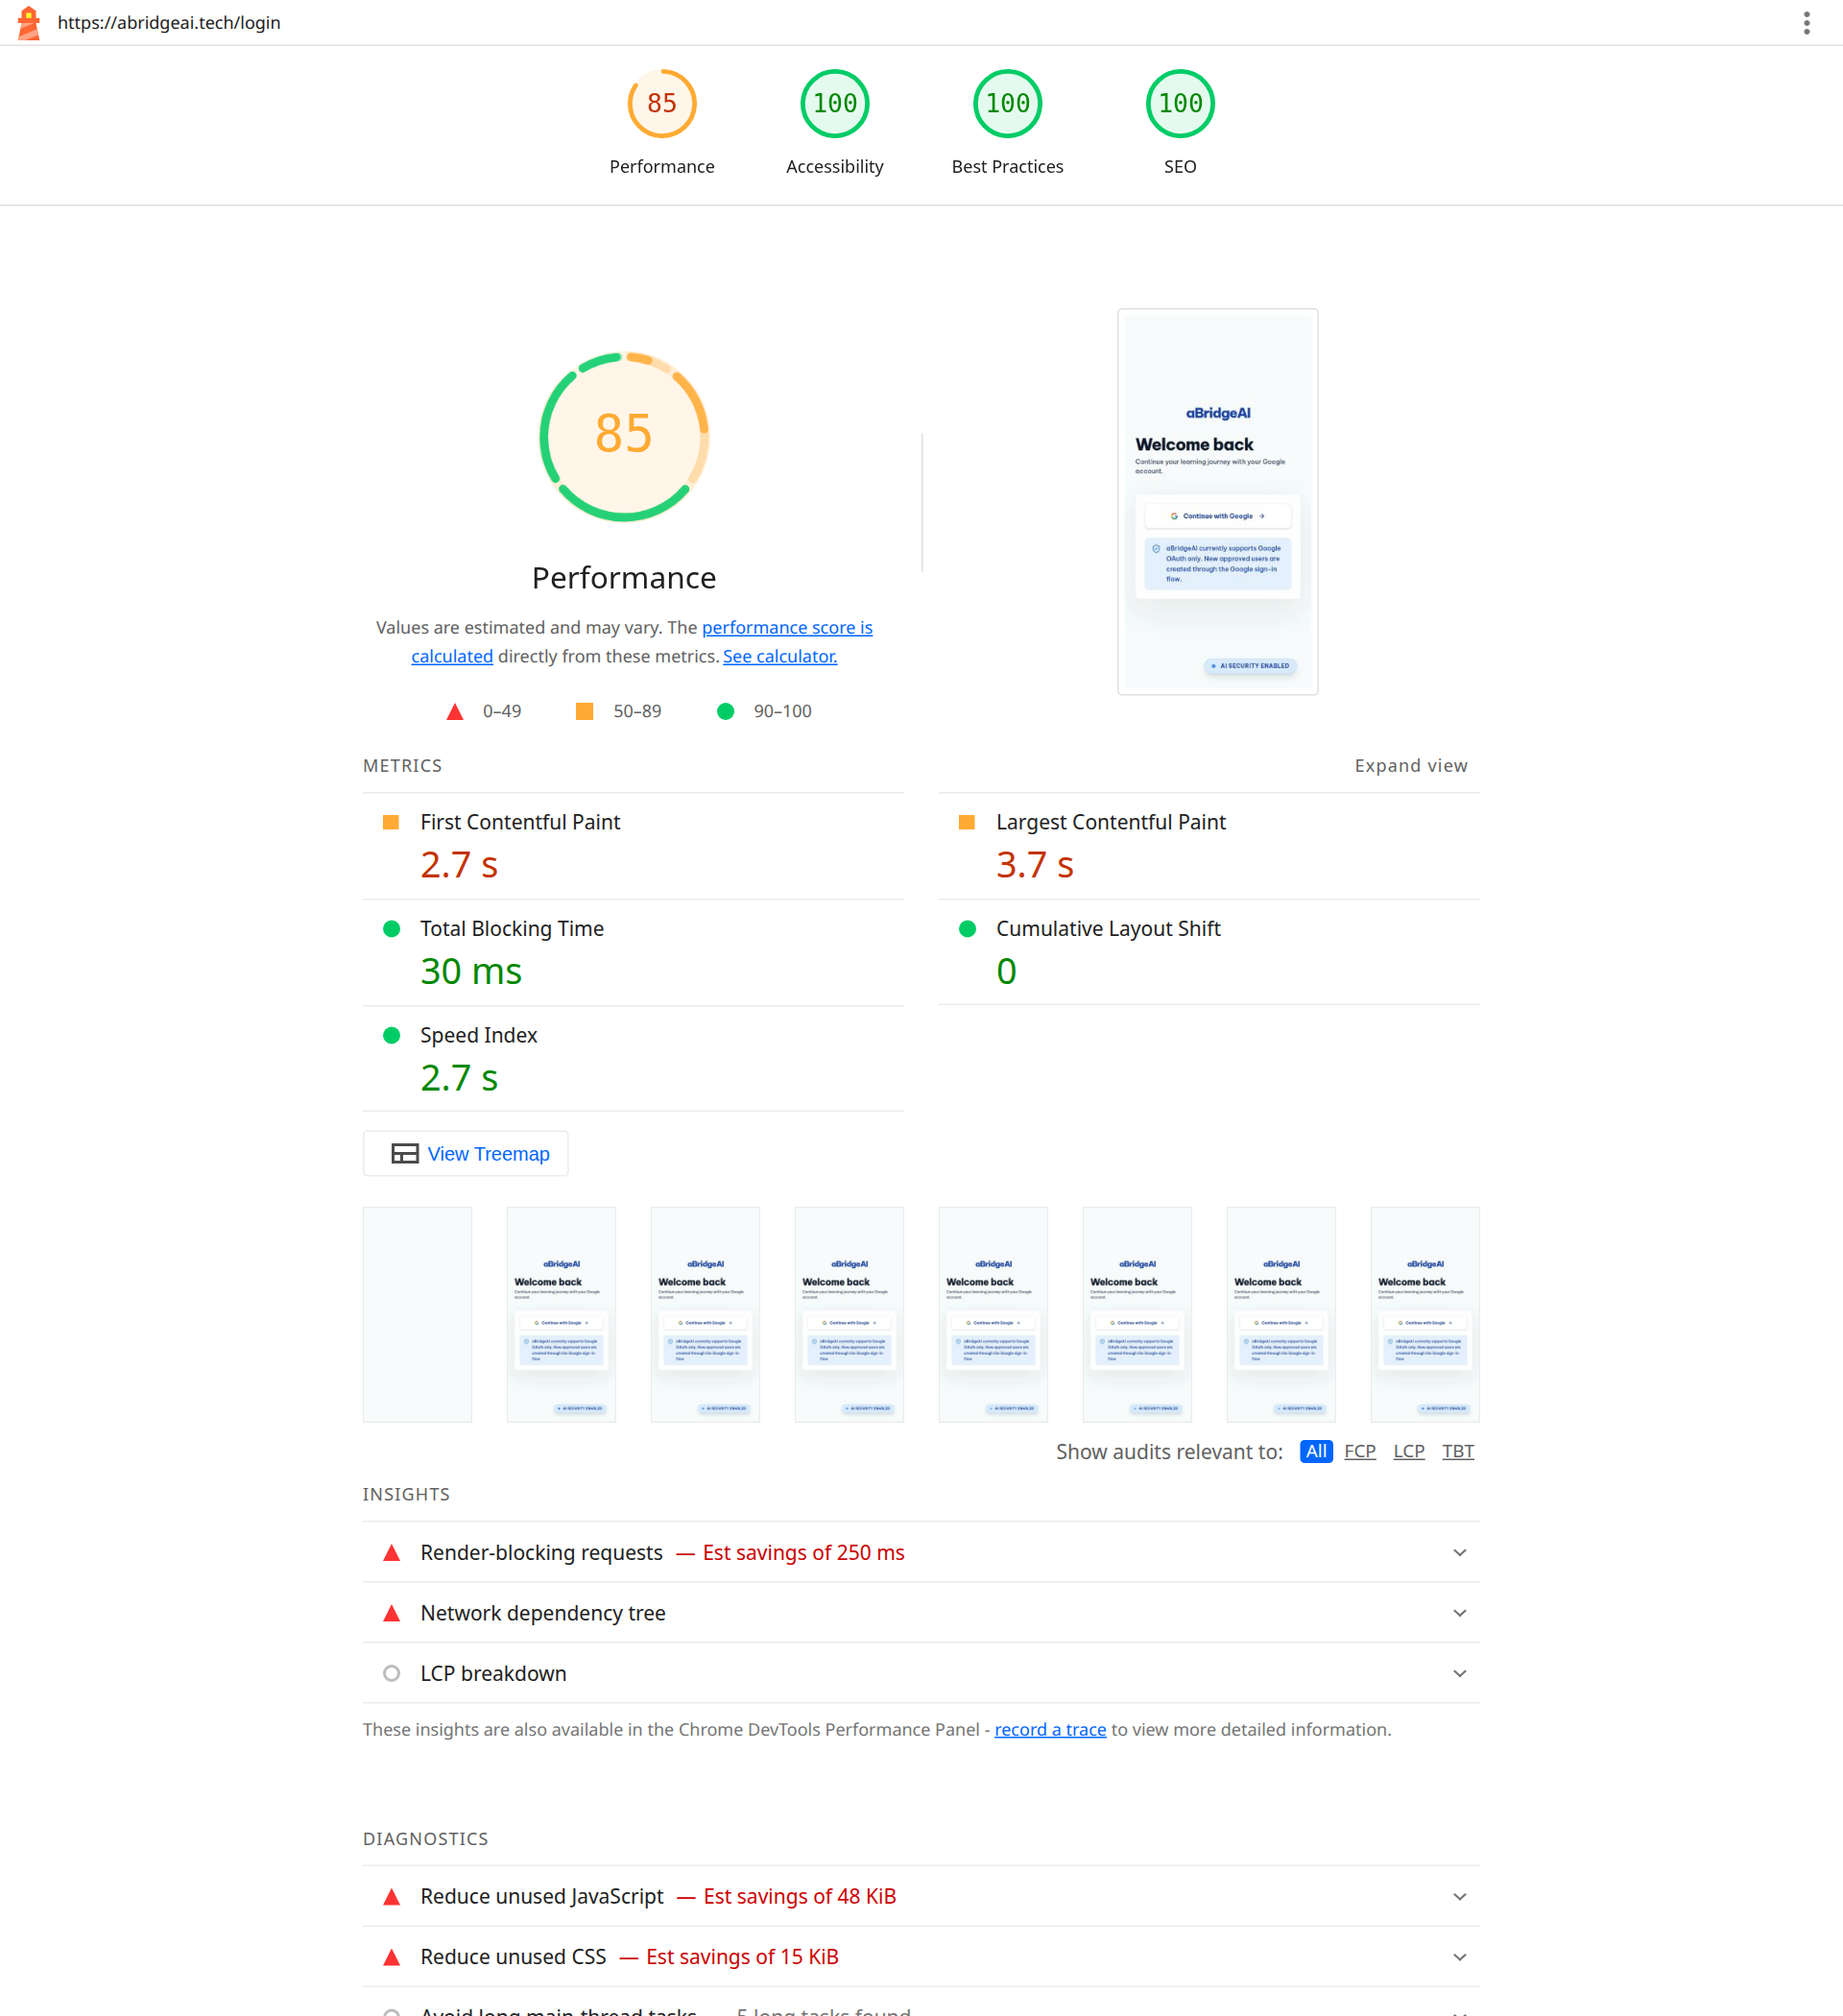
\includegraphics[width=0.9\textwidth]{graphics/lighthouse/login_scores.png}
    \caption{Lighthouse audit scores and metrics for the Login page (Performance 100, Accessibility 100, Best Practices 100, SEO 100).}
    \label{fig:lh_login_scores}
\end{figure}

% ────────────────────────────────────────────────────────────
\subsection{Student Dashboard}
% ────────────────────────────────────────────────────────────

\begin{figure}[H]
    \centering
    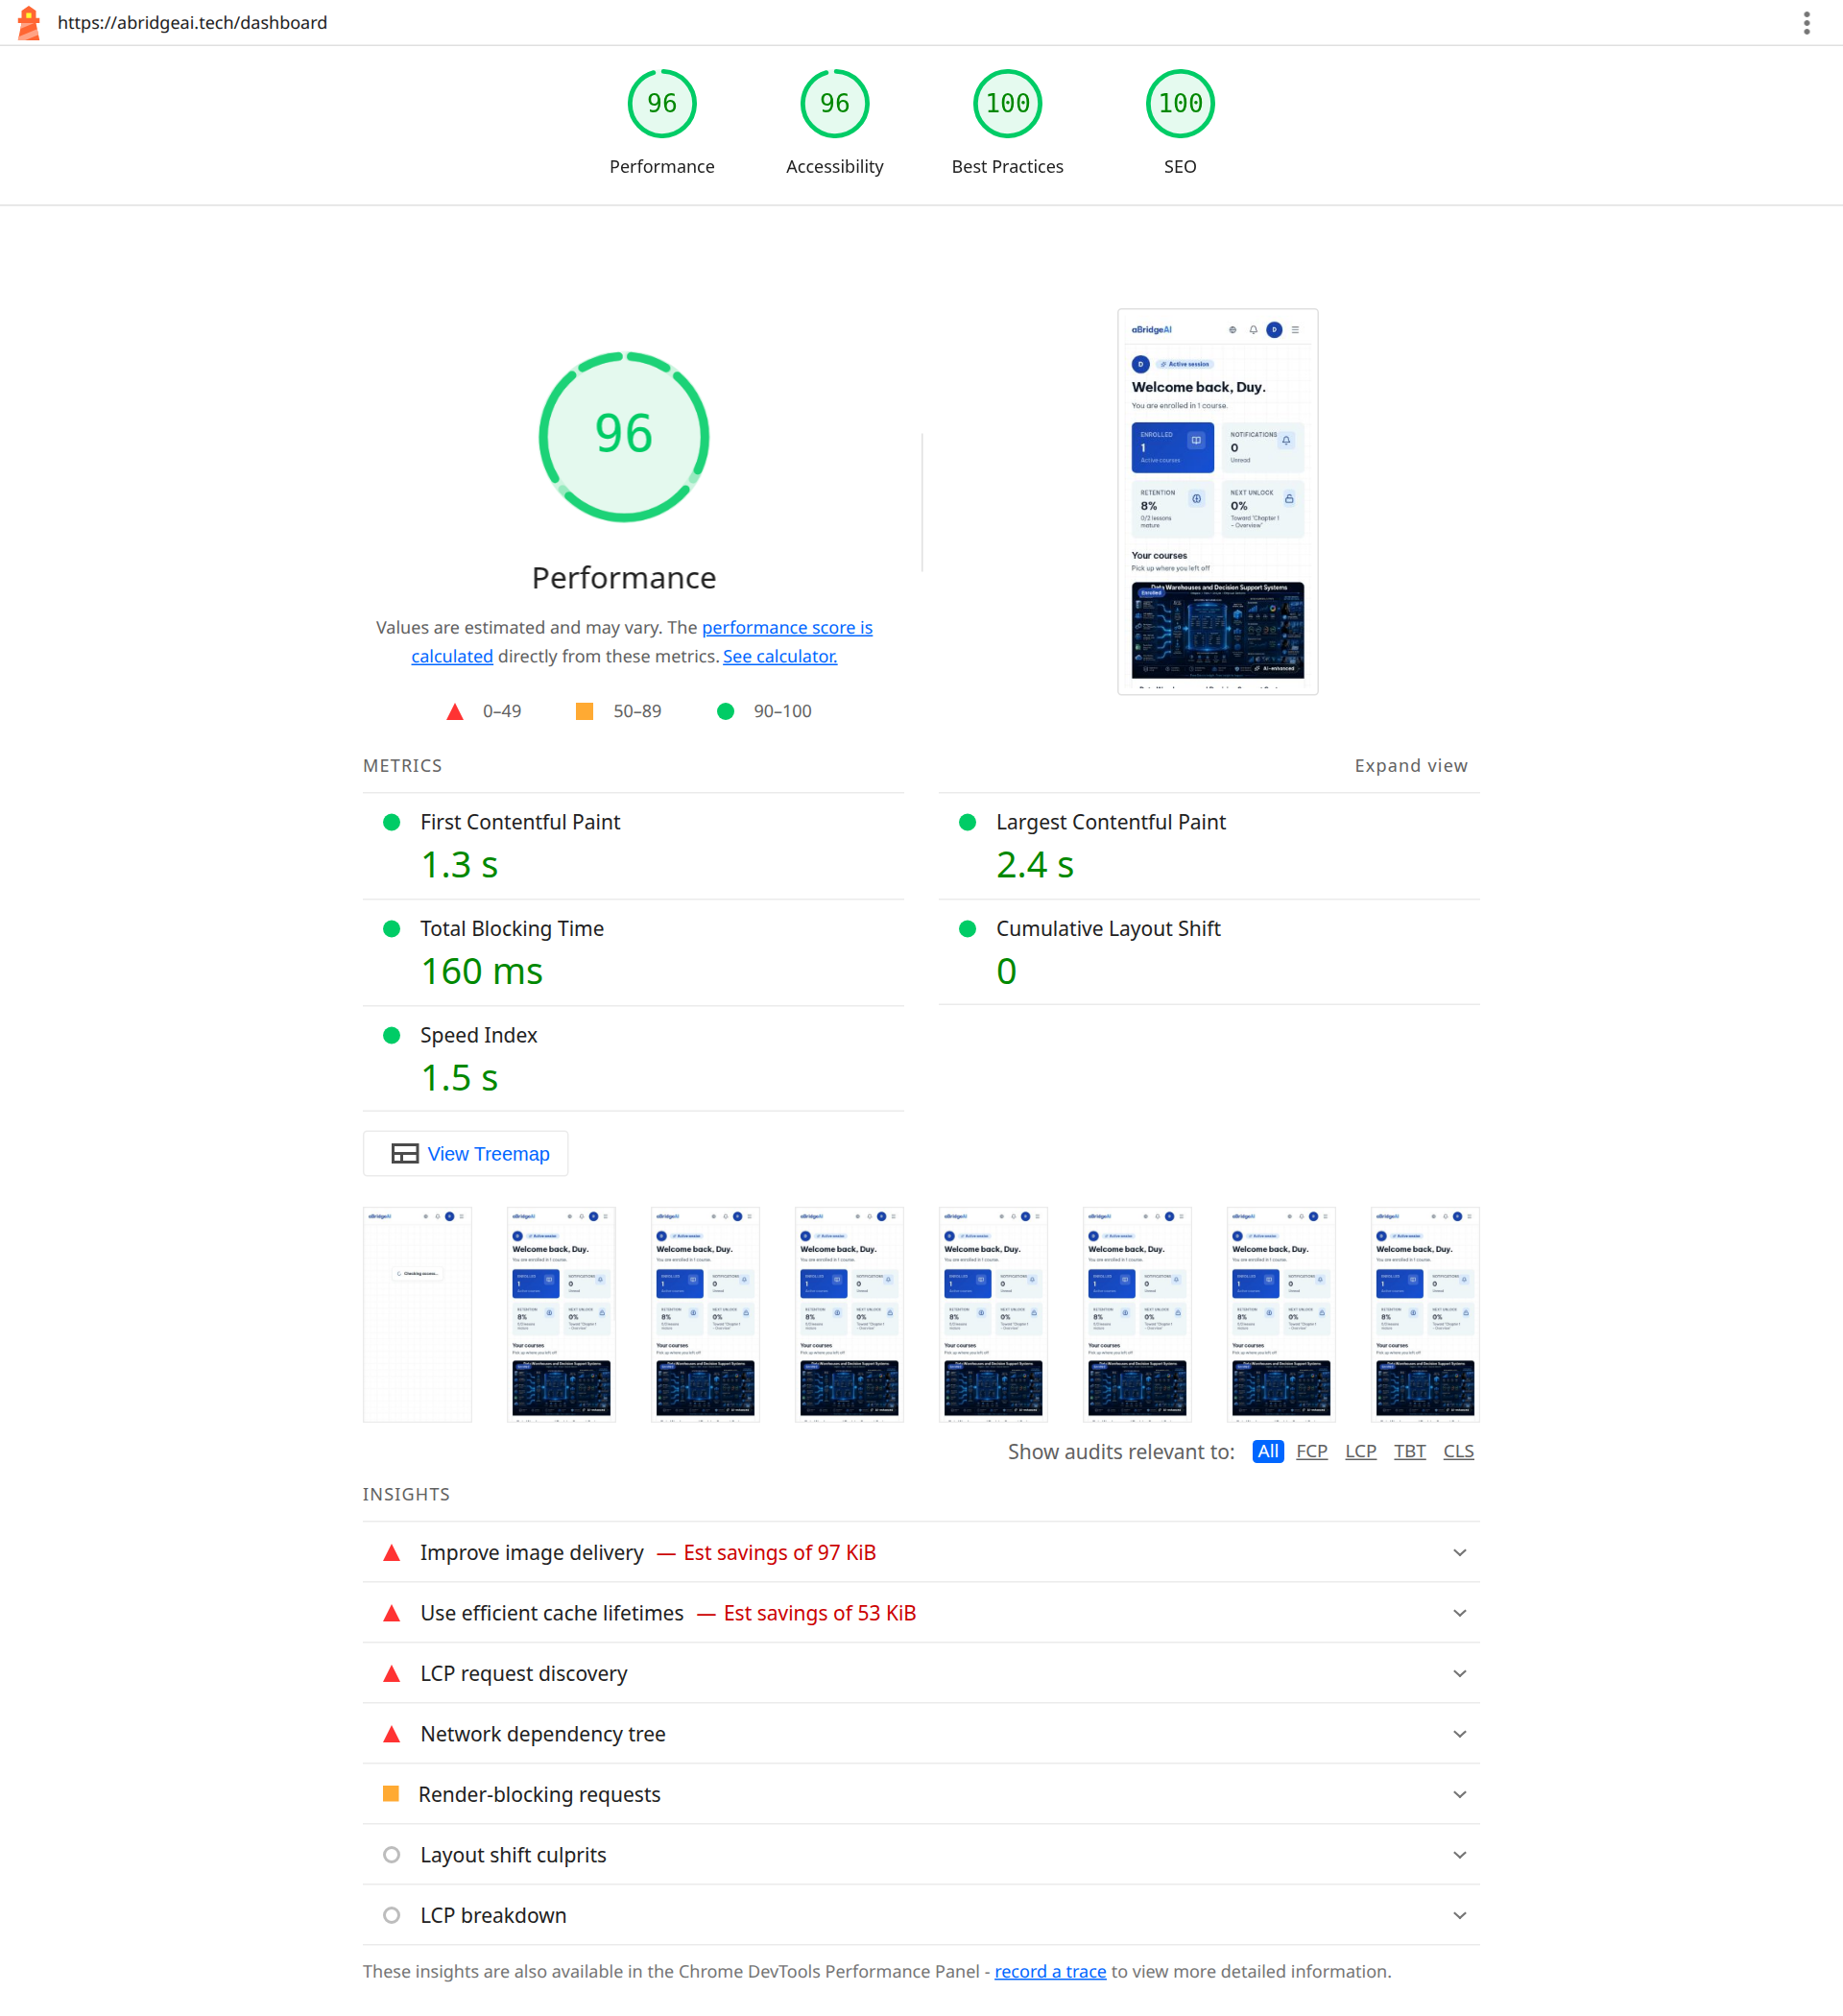
\includegraphics[width=0.9\textwidth]{graphics/lighthouse/dashboard_scores.png}
    \caption{Lighthouse audit scores and metrics for the Student Dashboard (Performance 100, Accessibility 96, Best Practices 100, SEO 100; CLS 0.006).}
    \label{fig:lh_dashboard_scores}
\end{figure}

% ────────────────────────────────────────────────────────────
\subsection{My Courses}
% ────────────────────────────────────────────────────────────

\begin{figure}[H]
    \centering
    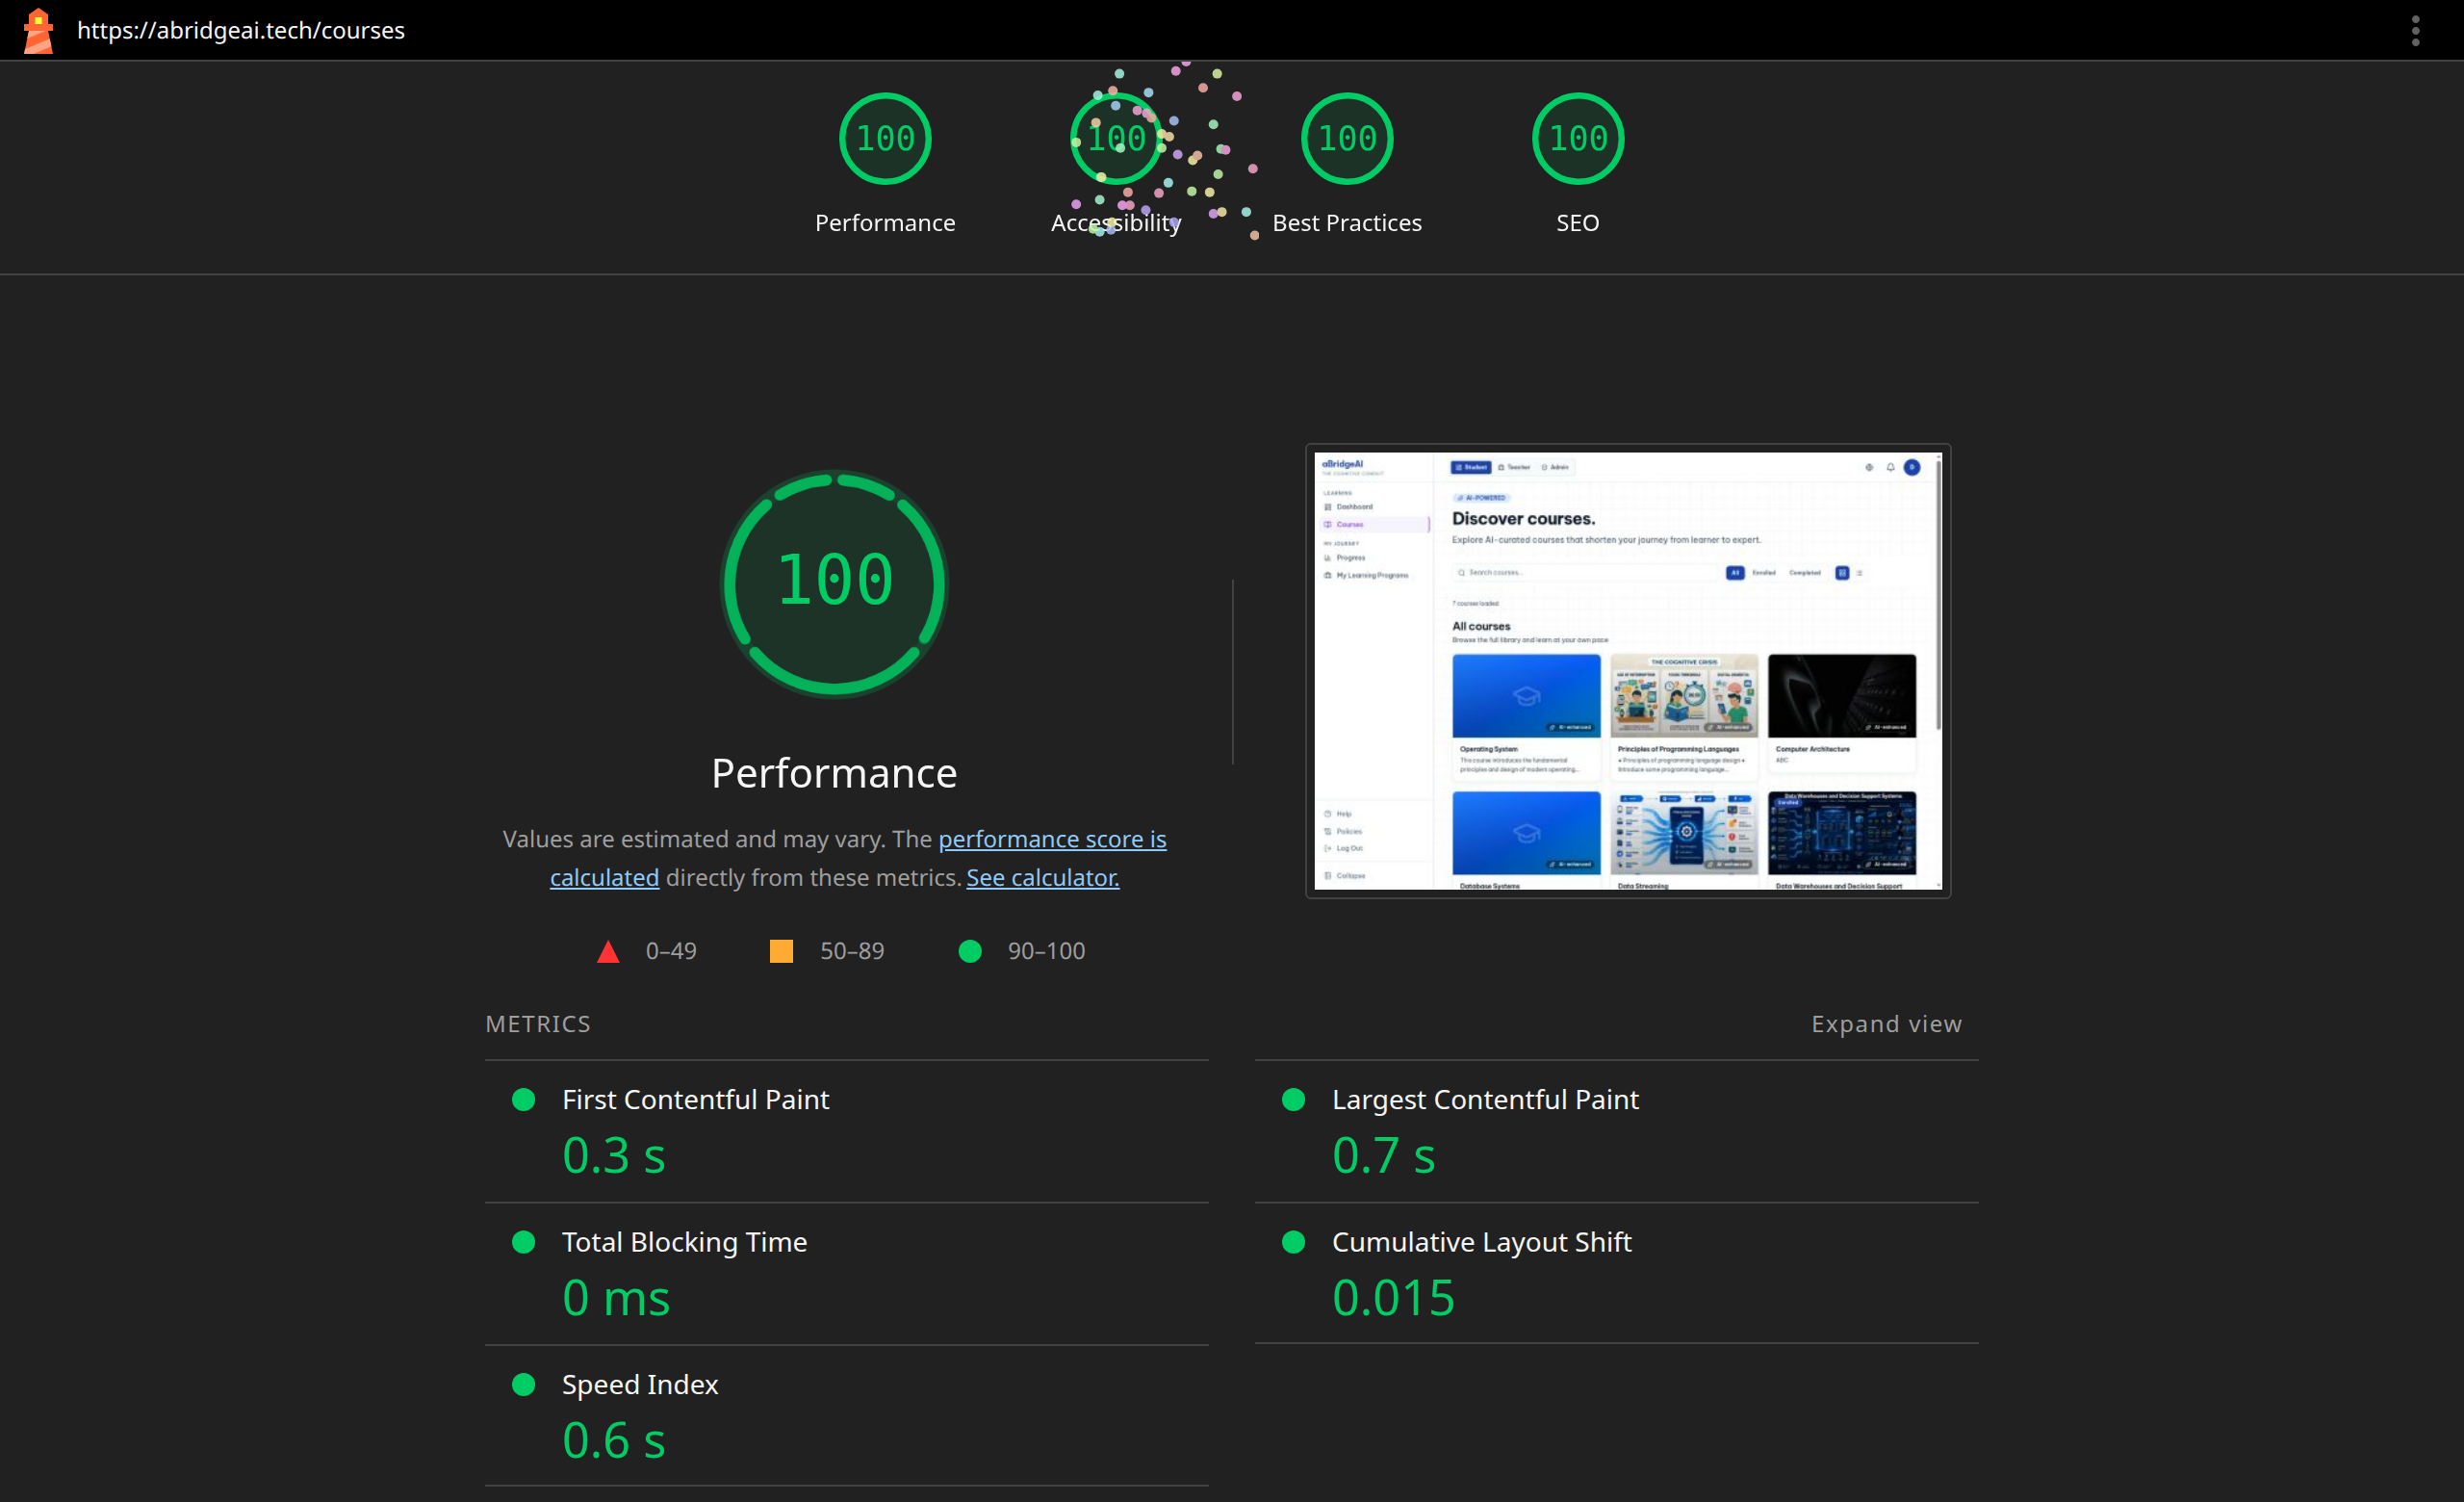
\includegraphics[width=0.9\textwidth]{graphics/lighthouse/courses_scores.png}
    \caption{Lighthouse audit scores and metrics for the My Courses page (Performance 100, Accessibility 100, Best Practices 100, SEO 100).}
    \label{fig:lh_courses_scores}
\end{figure}

% ────────────────────────────────────────────────────────────
\subsection{Course Detail}
% ────────────────────────────────────────────────────────────

\begin{figure}[H]
    \centering
    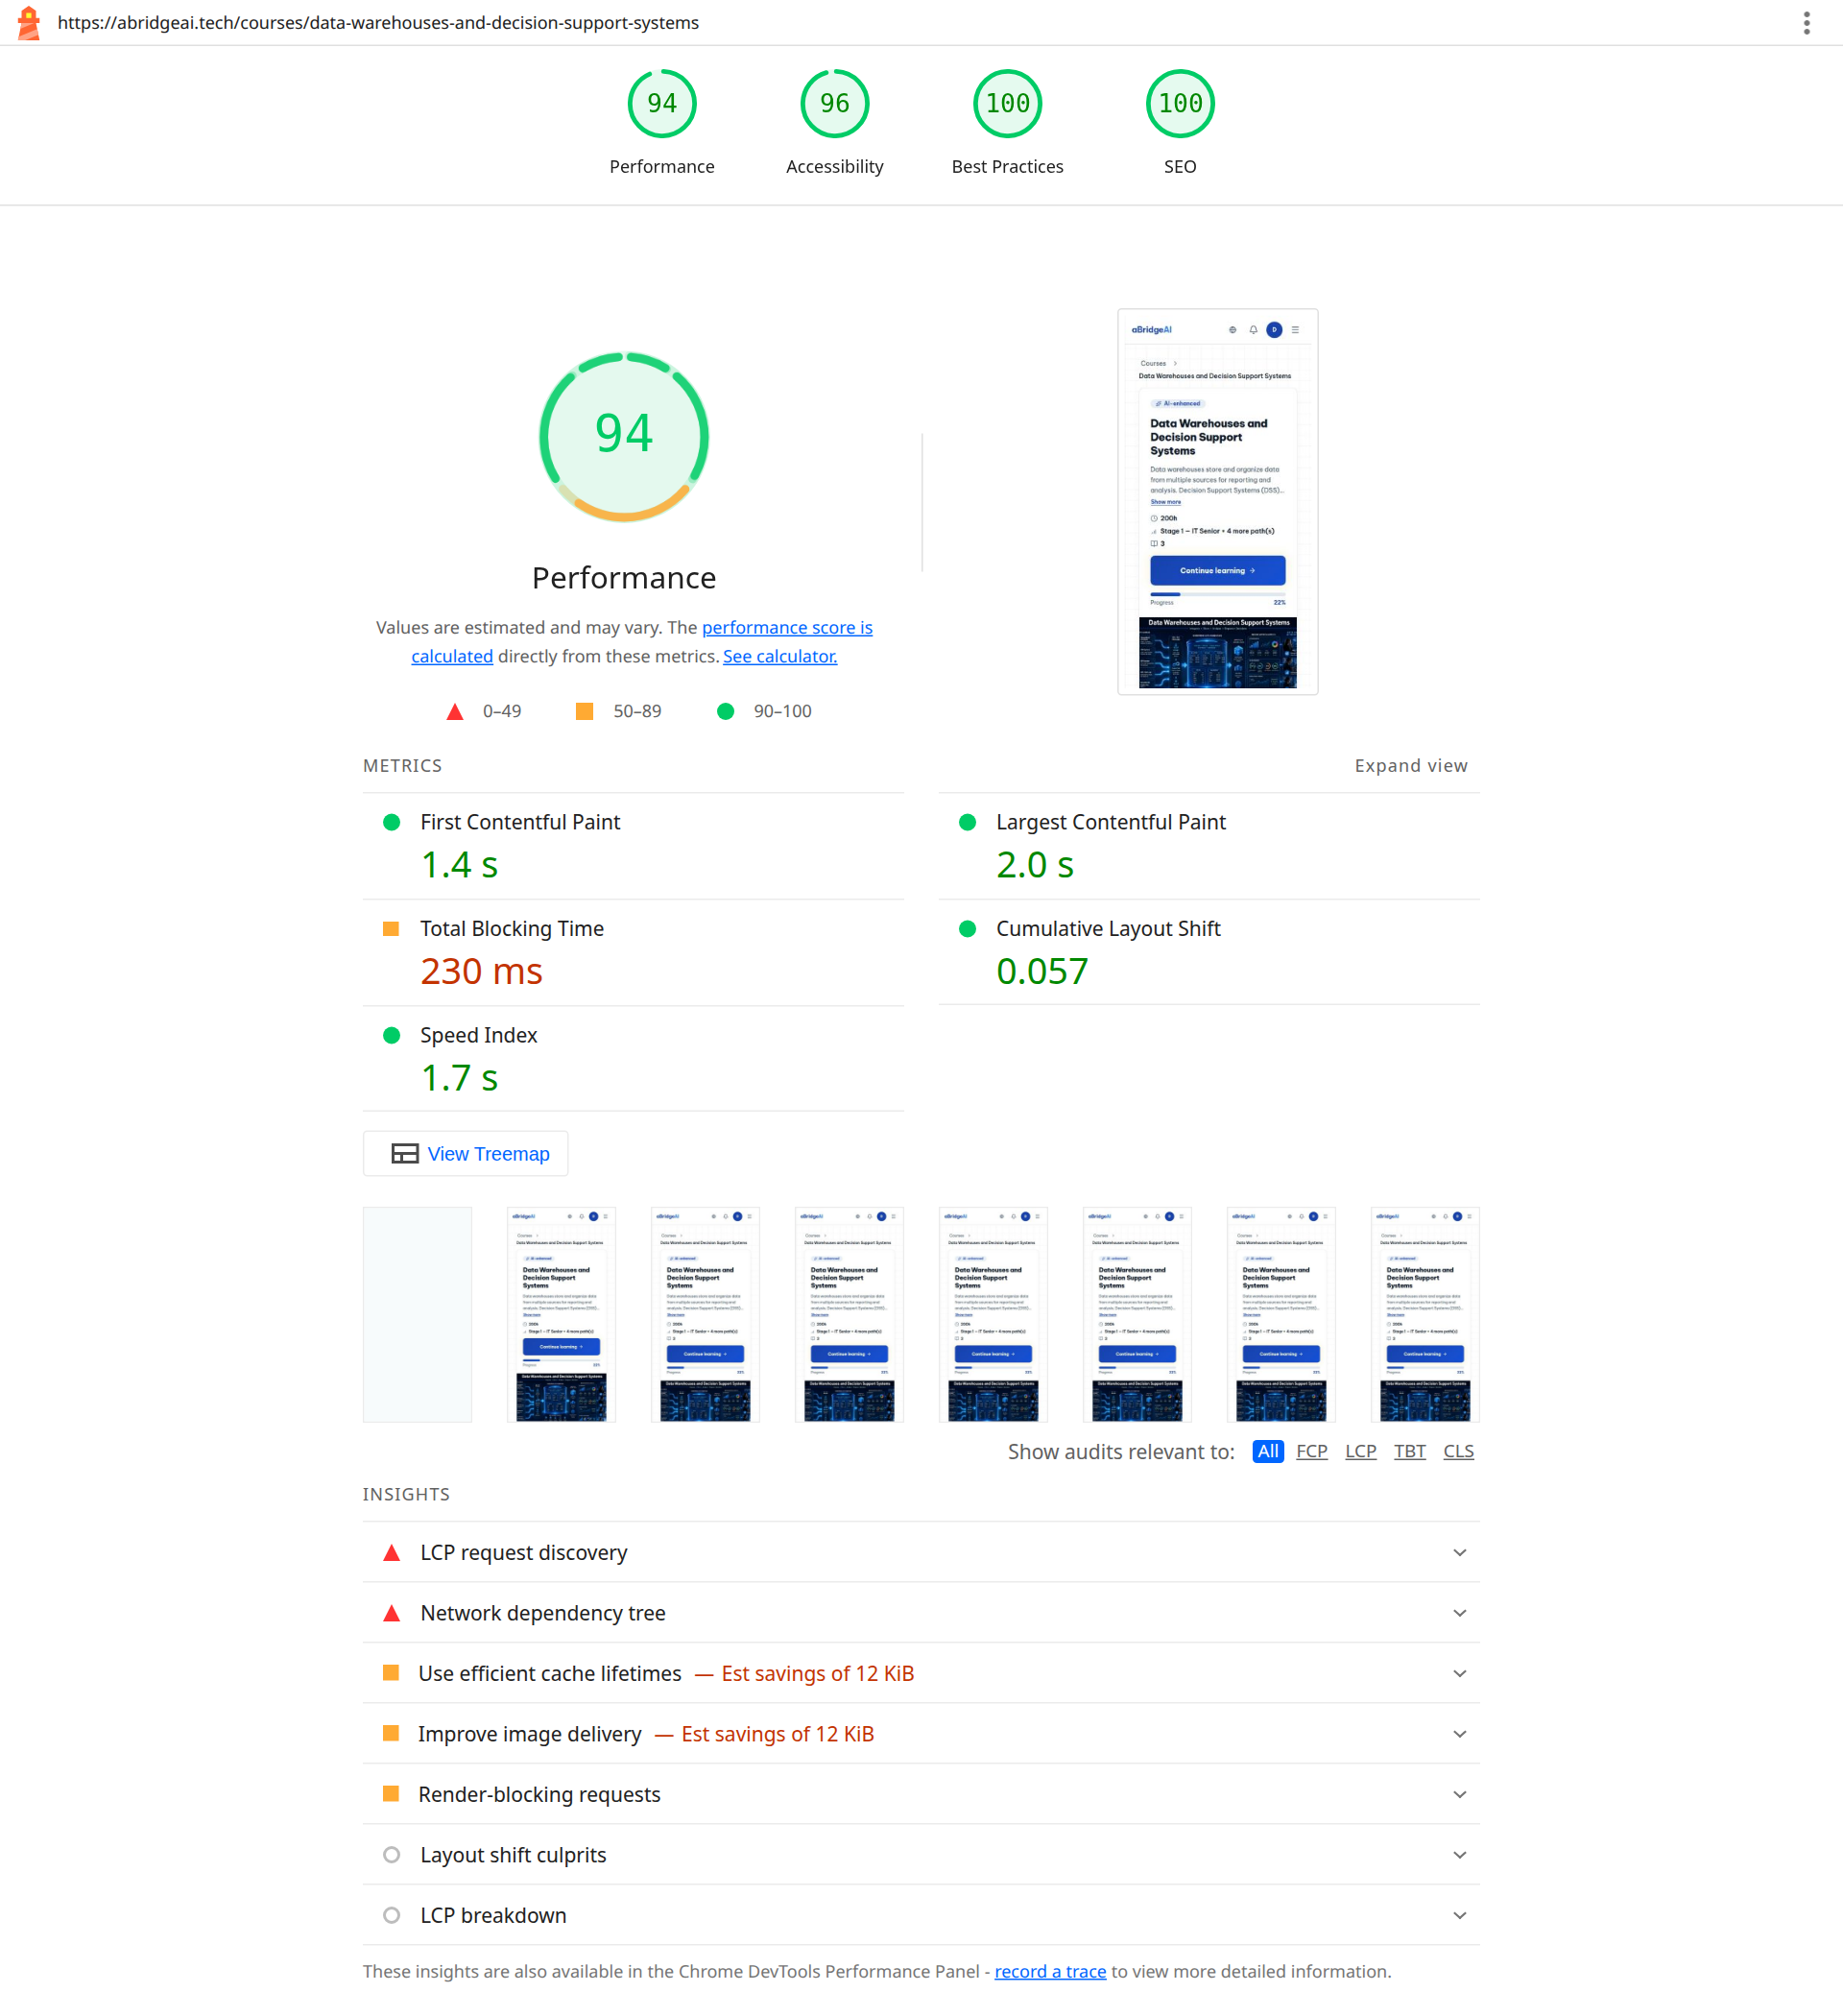
\includegraphics[width=0.9\textwidth]{graphics/lighthouse/course-detail_scores.png}
    \caption{Lighthouse audit scores and metrics for the Course Detail page (Performance 100, Accessibility 96, Best Practices 100, SEO 100).}
    \label{fig:lh_course_detail_scores}
\end{figure}

% ────────────────────────────────────────────────────────────
\subsection{Quiz Attempt Review}
% ────────────────────────────────────────────────────────────

\begin{figure}[H]
    \centering
    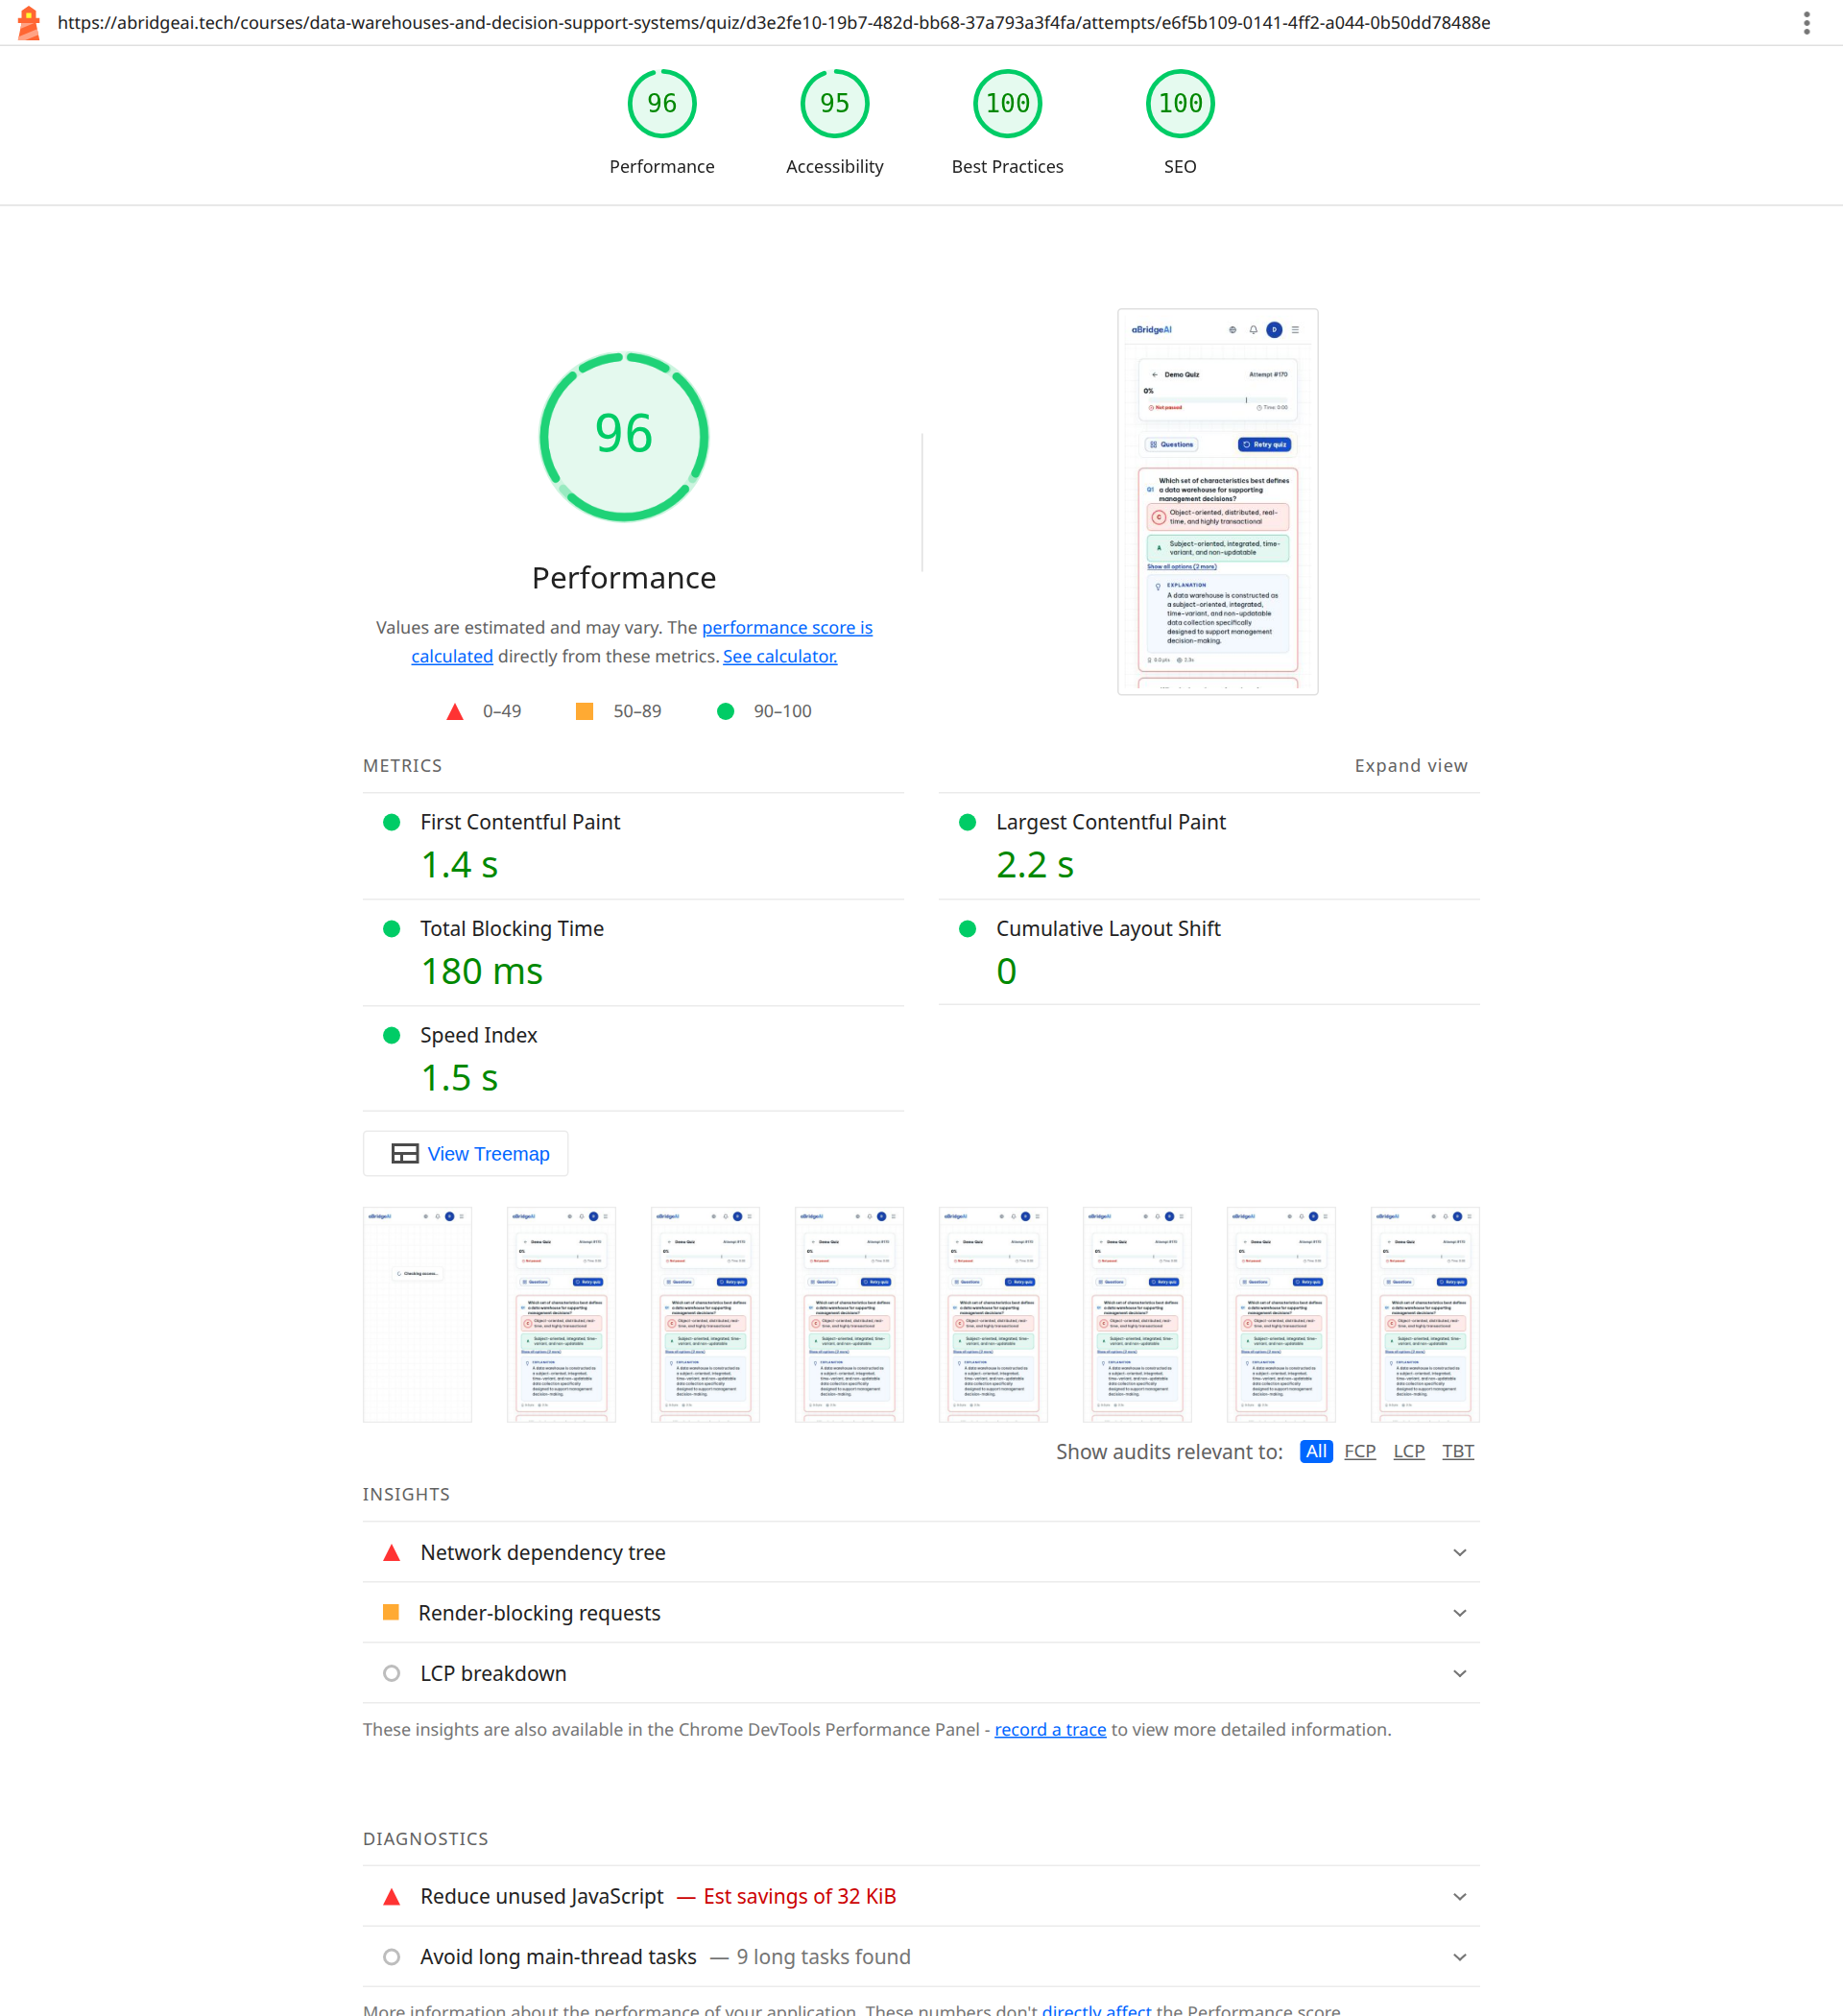
\includegraphics[width=0.9\textwidth]{graphics/lighthouse/quiz-attempt_scores.png}
    \caption{Lighthouse audit scores and metrics for the Quiz Attempt Review page (Performance 100, Accessibility 95, Best Practices 100, SEO 100).}
    \label{fig:lh_quiz_scores}
\end{figure}

\end{appendices}
